%%%%%%%%%%%%
%% Please rename this main.tex file and the output PDF to
%% [lastname_firstname_graduationyear]
%% before submission.
%%%%%%%%%%%%

\documentclass[12pt]{caltech_thesis}
\usepackage[hyphens]{url}
\usepackage{lipsum}
\usepackage{graphicx}
\usepackage{xcolor}
\usepackage{longtable}
\usepackage{pdflscape}
\usepackage{deluxetable}
\usepackage[CaptionAfterwards]{fltpage}
\usepackage{caption}

%\usepackage{todonotes}

%% Tentative: newtx for better-looking Times
\usepackage[utf8]{inputenc}
\usepackage[T1]{fontenc}
\usepackage{newtxtext,newtxmath}


% Must use biblatex to produce the Published Contents and Contributions, per-chapter bibliography (if desired), etc.
\usepackage[
    backend=biber,natbib,
    %backend=natbib,
    % IMPORTANT: load a style suitable for your discipline
    style=authoryear-comp,
    uniquelist=false,
    doi=False,
    uniquename=false,
    sortcites=false,
    %maxalphanames=1,
    %labelalpha,
    %sorting=nyt,
    bibstyle=apj, 
]{biblatex}
\renewcommand*{\nameyeardelim}{\addspace}
%\usepackage{natbib}
%\bibliographystyle{apj}
\newcommand{\todo}[3]{{\color{#2} \emph{#1} TO DO: #3}}
\newcommand{\btmtodo}[1]{\todo{BEN}{red}{#1}}

\renewcommand{\d}[1]{\ensuremath{\operatorname{d}\!{#1}}}
\newcommand{\rsun}{{R$_\odot$}}
\newcommand{\msun}{{M$_\odot$}}
\newcommand{\lsun}{{L$_\odot$}}
\newcommand{\kep}{{\textit {Kepler}}}
\newcommand{\itk}{{\textit {Kepler}}}
\newcommand{\KT}{{\textit {K2}}}
\newcommand{\WF}{{\textit {WFIRST}}}
\newcommand{\eg}{{\it e.g.}}
\newcommand{\ie}{{\it i.e.}}
\newcommand{\spitz}{{\textit {Spitzer}}}
\newcommand{\vsini}{{$V \sin i$}}
\newcommand{\teff}{$T_{\textrm eff}$}
\newcommand{\kms}{{km\,s$^{-1}$}}
\newcommand{\gcc}{{g\,cm$^{-3}$}}
\newcommand{\rstar}{{$R_\star$}}
\newcommand{\mstar}{{$M_\star$}}
\newcommand{\rhostar}{{$\rho_\star$}}
\newcommand{\logg}{{log(g)}}
\newcommand{\mh}{{[M/H]}~}
\newcommand{\feh}{{[Fe/H]}~}
\newcommand{\mearth}{{M$_\oplus$}}
\newcommand{\rearth}{{R$_\oplus$}}
\newcommand{\mjup}{{M$_\textrm{Jup}$}}
\newcommand{\rjup}{{R$_\textrm{Jup}$}}
\newcommand{\LA}{{LHS\,6343\,A}}
\newcommand{\LB}{{LHS\,6343\,B}}
\newcommand{\LC}{LHS\,6343\,C}
\newcommand{\LHS}{{LHS\,6343}}
\newcommand{\ira}{{3.6$\mu$m}}
\newcommand{\irb}{{4.5$\mu$m}}
\newcommand{\thisstarsix}{GJ\,3305}
\newcommand{\rprs}{{$R_p/R_{\star}$}}
\newcommand{\ars}{{$a/R_{\star}$}}
\newcommand{\project}[1]{\textsl{#1}}
\newcommand{\Ci}{Campaign~1}
\newcommand{\afe}{{[$\alpha$/Fe]}~}
\newcommand{\dd}{{\ensuremath{\,\mathrm{d}}}}
\newcommand{\paperip}{\citep{Foreman-Mackey15}}
\newcommand{\paperit}{\citet{Foreman-Mackey15}}

\newcommand{\Nfp}{6}
\newcommand{\Nvalidated}{21}
\newcommand{\Nlimbo}{9} %adds up to 36
\newcommand{\Nvalnew}{17} % 4 previously validated



\newcommand{\procspie}{Proc. SPIE}
\newcommand{\aj}{AJ}
\newcommand{\pasp}{PASP}
\newcommand{\apj}{ApJ}
\newcommand{\apjl}{ApJL}
\newcommand{\apjs}{ApJS}
\newcommand{\aap}{A\&A}
\newcommand{\mnras}{MNRAS}
\newcommand{\sci}{Science}
\newcommand{\nat}{Nature}
\newcommand{\aapr}{A\&A Rev.}
\newcommand{\actaa}{Acta Astronomica}
\newcommand{\araa}{ARA\&A}
\newcommand{\aaps}{A\&AS}
\newcommand{\planss}{Planet. Space Sci.}
\newcommand{\icarus}{Icarus}

% Name of your .bib file(s)
\addbibresource{exopapers.bib}


\begin{document}

% Do remember to remove the square bracket!
\title{Low-Mass Stars and Their Companions}
\author{Benjamin Tyler Montet}

\degreeaward{Doctor of Philosophy}                 % Degree to be awarded
\university{California Institute of Technology}    % Institution name
\address{Pasadena, California}                     % Institution address
\unilogo{caltech.png}                                 % Institution logo
\copyyear{2017}  % Year (of graduation) on diploma
\defenddate{July 18, 2016}          % Date of defense

\orcid{0000-0001-7516-8308}

\rightsstatement{All rights reserved except where otherwise noted}


\maketitle[logo]


\begin{acknowledgements} 	 
I am extremely grateful to everyone who has helped me get to Caltech, as well as those
who have helped me through these past five years.
Of course, this list must begin with my parents: thank you for all your support and
encouragement over the past 27 years.
I also want to thank my fifth grade teacher, Mrs.\ Kim Klappauf, for always being so
enthusiastic and showing us that being into science was cool.

I want to thank my advisor, John Johnson, and everyone involved in the Exolab during 
my time. 
That (long!) list includes Justin Crepp, Phil Muirhead, Leslie Rogers,
Brendan Bowler, Jennifer Yee, and Luan Ghezzi for allowing them to regularly bug them with
questions in their offices.
I especially want to thank Jon Swift for his patience in working through problems on the
white board, his pedantry in third order corrections, and his enthusiasm for life both
inside and out of Cahill.

I want to thank everyone involved with the Summer 2013 ``Modern Statistical and
Computational Methods for Analysis of Kepler Data'' workshop at the Statistical and
Applied Mathematical Sciences Institute in Research Triangle Park, North Carolina.
The workshop certainly changed the trajectory of my thesis, and allowed me to meet 
new friends and collaborators. 
I thank the organizers, especially Eric Ford and David Hogg (the latter whom, I
acknowledge formally,
I still owe a bottle of good wine), for allowing me to participate, and the participants
for being so amazing, especially Ruth, Dan, Robert, Megan, Ben, Angie, and Gal.

I want to thank the Caltech Astronomy graduate students for being the friendliest, 
most pleasant classmates and friends one could ask for. 
I particularly want to thank (in no particular order) Mislav, Antonija, Trevor, Allison, Yi, Matt, Sirio,
Gwen, Drew, Ryan and Donal. 
To my officemates Walter, Shriharsh, Drew, Sirio, and Mislav: thank you for putting up
with me. Sorry I took away your couch (if it's any consolation, it looks nice in my 
apartment.)
I also want to thank the faculty for allowing the graduate community to be what it is, 
especially Wal Sargent. I still miss seeing your face around the department and hearing
your opinions on everything from iced tea to camping. And football, especially football.

I will always remember the traditions shared among the Cahill grad students: 
ski trips to Mammoth (never Big Bear, sorry Trevor), Wednesday night softball with the Big Bangers,
Halloween parties, trips to the Athenaeum, wine and cheese, concerts at the Hollywood
Bowl, finding space for 15 people to eat lunch together at Chandler, and so much more.

I would like to thank my committee: Heather Knutson, Gregg Hallinan, Phil Hopkins, and
Tony Readhead for reading my thesis (at least this far) and for their support and
guidance.
I also want to thank Patrick Shopbell, Anu Mahabal, and Jos\'e Calderon, who must form
the best computing staff in all of astronomy.

Finally, I want to thank Laura. Thank you for your support. 
Thank you for always being there when I need someone.
Thank you for always being there when I need someone to put me in my place.
I've enjoyed every day of our adventure, and I can't wait to see what happens next.
   
   
\end{acknowledgements}

\begin{abstract}
In this thesis, I present seven studies aimed towards better understanding the demographics
and physical properties of M dwarfs and their companions.
These studies focus in turn on planetary, brown dwarf, and stellar companions to M dwarfs.

I begin with an analysis of radial velocity and transit timing analyses of multi-transiting
planetary systems, finding that if both signals are measured to sufficiently high precision
the stellar and planetary masses can be measured to a high precision, eliminating a need
for stellar models which may have systematic errors.
I then combine long-term radial velocity monitoring and a direct imaging
campaign to measure the occurrence rate of giant planets around M dwarfs.
I find that $6.5\% \pm 3.0\%$ of M dwarfs host a Jupiter mass or larger planet within
20 AU, with a strong dependence on stellar metallicity.

I then present two papers analyzing the LHS\,6343 system, which contains a widely
separated M dwarf binary (AB).
Star A hosts a transiting brown dwarf (LHS\,6343\,C) with a 12.7 day period.
By combining radial velocity data with transit photometry, I am able to measure
the mass and radius of the brown dwarf to 2\% precision, the most precise measurement
of a brown dwarf to date.
I then analyze four secondary eclipses of the LHS\,6343\,AC system as observed by \spitz\
in order to measure the luminosity of the brown dwarf in both \spitz\ bandpasses.
I find the brown dwarf is consistent with theoretical models of an 1100 K T dwarf at an
age of 5 Gyr and empirical observations of field T5-6 dwarfs with temperatures of 
$1070 \pm 130$ K.
This is the first non-inflated brown dwarf with a measured mass, radius, and multi-band
photometry, making it an ideal test of evolutionary models of field brown dwarfs.

Next, I present the results of an astrometric and radial velocity campaign to measure the
orbit and masses of both stars in the GJ\,3305\,AB system, an M+M binary comoving with
51\,Eridani, a more massive star with a directly imaged planetary companion.
I compare the masses of both stars to largely untested theoretical models of young M 
dwarfs, finding that the models are consistent with the measured mass of star A but 
slightly overpredict the luminosity of star B.

In the final two science chapters I focus on space-based transit surveys, present and
future.
First, I present the first catalog of statistically validated planets from the \KT\ mission, as well as updated stellar and planetary parameters for all systems with candidate
planets in the first \KT\ field.
The catalog includes K2-18b, a ``mini-Neptune'' planet that receives a stellar insolation
consistent with the level that the Earth receives from the Sun, making it a useful
comparison against planets of a similar size that are highly irradiated, such as GJ\,1214\,b.
Finally, I present predictions for the \textit{WFIRST} mission. 
While designed largely as a microlensing mission, I find it will be able to detect
as many as 30,000 transiting planets towards the galactic bulge, providing
information about how planet occurrence changes across the galaxy.
These planets will be able to be confirmed largely through direct detection of their
secondary eclipses.
Moreover, I find that more than 50\% of the planets it detects smaller than Neptune 
will be found around M dwarf hosts.



\end{abstract}

%% Uncomment the `iknowhattodo' option to dismiss the instruction in the PDF.
%\begin{publishedcontent}%[iknowwhattodo]
% List your publications and contributions here.
%\nocite{Cahn:etal:2015}
%\end{publishedcontent}

\tableofcontents
\listoffigures
\listoftables
%\printnomenclature

\mainmatter

\chapter{Introduction}

\section{The M Dwarf Spectral Class}
For thousands of years, humans have studied stellar astronomy. 
The ancient Greeks, especially Hipparchos, measured the brightness and position of hundreds 
of stars.
The ancient Egyptians used observations of stars, particularly Sirius and Thuban, to measure
time for agricultural purposes.
The ancient Chinese observed supernovae for divination purposes.
Stars are one of the primary ways we can observe the universe. 
On large scales, the galaxies we observe at high redshifts are made up of stars;
on small scales, the asteroids we observe in our solar system are observable because they are
reflecting light from our
own sun.
In these cases, we can only understand the astrophysical phenomena we observe because we 
understand the starlight that creates these phenomena.

Different stars are divided into different spectral classes based on their observable spectroscopic
features.
Type M dwarfs were a part of the original Draper Catalogue of Stellar Spectra \citep{Pickering90}, 
classified as having weak but non-zero hydrogen absorption features in their spectra.
The system was alphabetical: they were classified between K and O stars, 
the former having stronger hydrogen absorption and the latter none at all.
With the development of the Harvard system, \citet{Cannon01} preserved the M spectral class and placed it
at one end of the classification system, next to K stars.
We now know that M and O stars have little hydrogen absorption in their atmospheres for very different reasons
and the modern classification system maps stellar effective temperature: M dwarfs are the coolest main-sequence
stars and the least massive hydrogen burning stars in the galaxy.
Today, the boundary between K and M dwarfs is defined by the presence of titanium oxide (TiO) bands in the
atmospheres of M dwarfs \citep{Kuiper38, Morgan38}, which can form when a star's effective temperature is below approximately 3500 K.

The single classification for M dwarfs can give the appearance of M dwarfs as a single, monolithic block.
Indeed, this is largely true for other spectral types.
The Sun has a radiative core, in which nuclear reactions are dominated by the p-p chain, and a convective 
outer layer, which contributes to the existence of a magnetic field.
The same is true for stars from the middle of the F spectral class through early M dwarfs.
M dwarfs, meanwhile, have an incredible diversity.
The M dwarf class spans an order of magnitude in mass, 
an order of magnitude in radius, and
a factor of 40 in luminosity \citep{Veeder74}.
There are significant changes in the structure of the stars across this class as well.
Below approximately 0.35 \msun, M dwarfs become fully convective, leading to a
rapid decrease in the radius and luminosity of stars just below this boundary \citep{Chabrier97}.
At the late edge of the M dwarf class are brown dwarfs, objects without high enough central densities to 
fuse hydrogen. 

In terms of their structure, F7 and K3 
dwarfs have more in common than M0 and M9 dwarfs.
Some of the stars even vary in time.
As a brown dwarf leaves the T Tauri stage of stellar evolution it has a temperature of approximately 3000 K
and a spectrum consistent with that of a mid-M dwarf.
Brown dwarfs then cool and evolve into ``late-type'' L, T, and eventually Y dwarfs at a rate 
which depends on their mass.
I will discuss the evolution of brown dwarfs more fully in Section \ref{sec:BDs}.
If the abundance of M dwarfs and the diversity of their structure had been understood at the time of the development 
of the Harvard stellar classification system, it is possible that these stars would have been awarded more than a 
single spectral type.






\section{M Dwarfs: The Silent Majority}
The early work on stellar spectroscopic classification of type M stars is based on
spectroscopy of M giants. 
The
Draper catalogue was first published in 1890 and the
Harvard stellar classification scheme in 1901,
but 
the first spectrum of an M dwarf was obtained only 100 years ago when 
\citet{Adams13} collected an observation of the M+M binary Groombridge 34.
This 8th magnitude star was known to be peculiar relative to the M stars with known spectra because of its 
high proper motion of 3 arcseconds per year; today we know it is within 4 parsec of the Sun.

The oldest known surviving diagram plotting stellar absolute magnitude against spectral type \citep{Russell14}, now known as a Hertsprung-Russell Diagram, includes hundreds of stars, as shown in Figure \ref{fig:HR}.
Today we know that M dwarfs make up approximately 75\% of the stars in the galaxy,
yet only $\sim$5\% of the stars included in Russell's figure are listed as
spectral type M. These stars are absent in the original work because they are
intrinsically faint.



\begin{figure}[hbt!]
\centering
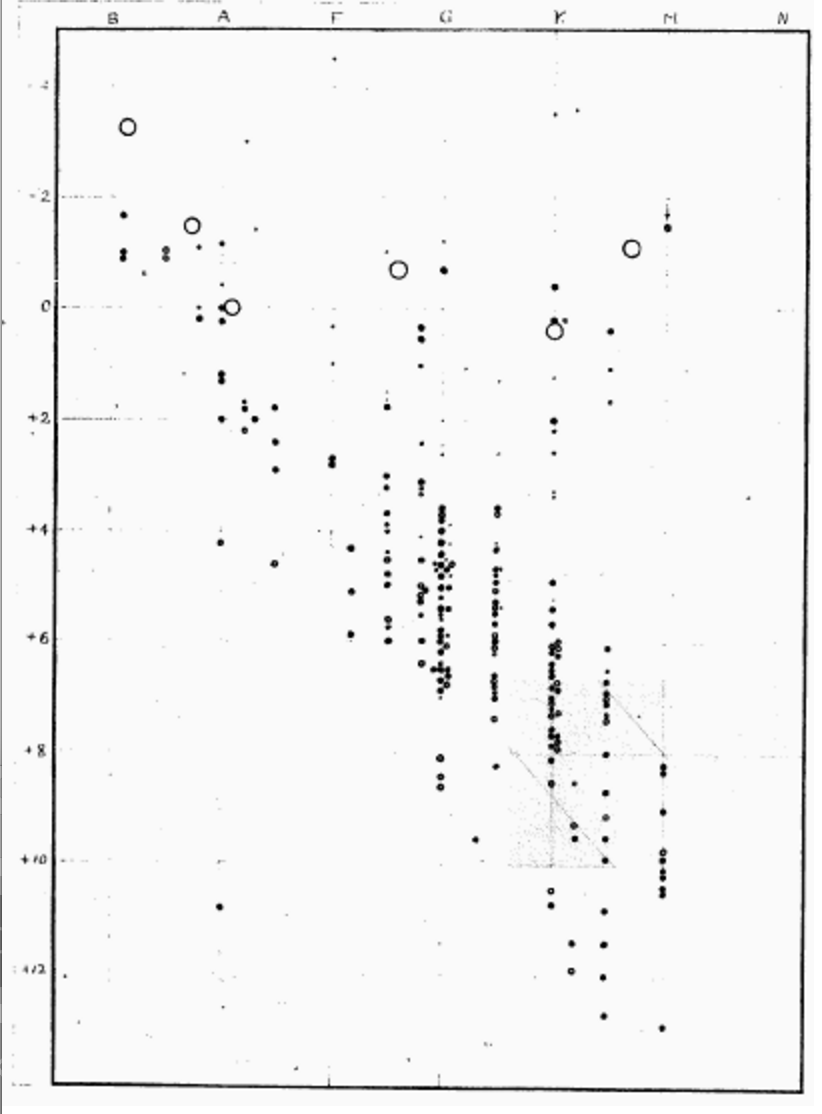
\includegraphics[width=.5\textwidth]{chapter1/hr.png}
\caption[Russell's original H-R Diagram]{The original H-R diagram, as published by
\citet{Russell14}. On the $y$-axis is absolute magnitude, equivalent to the logarithm
of the star's luminosity. On the $x$-axis is stellar spectral type, which we now know
maps approximately to stellar effective temperature.}
\label{fig:HR}
\end{figure}

The faintness of M dwarfs is the result of the physics of their interior, 
specifically the stellar mass-luminosity relation.
To show this, let us begin with the equations of stellar structure.
The first of these declares a star is in hydrostatic equilibrium:
\begin{equation}
\frac{\d P(r)}{\d r} = - \frac{ G m \rho}{r^2 },
\label{eq:hydro}
\end{equation}
where $P(r)$ is the pressure exerted on a particle at a radius $r$, $G$ is Newton's
constant, $m$ the mass enclosed inside the radius $r$, and $\rho$ the stellar density,
itself a function of radius as well.

The second equation defines mass conservation:
\begin{equation}
\frac{\d m(r)}{\d r} = 4 \pi r^2 \rho,
\end{equation}
where $\pi$ is the ratio of a circle's circumference to its diameter,
and all other variables retain their meaning from Equation \ref{eq:hydro}.

The third equation defines energy transport:
\begin{equation}
\frac{\d L(r)}{\d r} = 4 \pi r^2 \rho \epsilon,
\end{equation}
where $L$ is the energy leaving a spherical shell of radius $r$, produced by the
material in the star interior to $r$ and $\epsilon$ is the energy released per unit
mass per second inside the star.

The final equation defines the temperature gradient inside a star. 
The exact form of this equation depends on the method for which energy is transported
inside the star.
For radiative transport, the temperature gradient is
\begin{equation}
\frac{\d T}{\d r} = - \frac{3}{4ac} \frac{\bar{\kappa} \rho}{T^3} \frac{L}{4\pi r^2}.
\end{equation}
Here, $T$ is the temperature of the star at a radius $r$, $ac$ is the radiation constant multiplied by the speed of light, also equal to four times the Stefan-Boltzmann
constant, and $\bar{\kappa}$ the mean opacity of the material.

Very low-mass stars are fully convective, not radiative, and therefore follow
a different limit:
\begin{equation}
\frac{\d T}{\d r} =  \bigg( 1 - \frac{1}{\gamma}\bigg)\frac{T}{P}\frac{\d P(r)}{\d r},
\end{equation}
where $\gamma$ is the adiabatic index, and is $5/3$ for a monatomic ideal gas,
and all other terms retain their previous meaning.

Let us consider two other proportionalities. First, we assume that the energy generation rate
inside a star is a function of its temperature and density:
\begin{equation}
\epsilon = \epsilon_0 \rho T^\nu
\end{equation}
where $\nu$ depends on the particular fusion pathway that is dominant in the core of
the star.
Second, we assume that the ideal gas law holds:
\begin{equation}
P \propto \rho T.
\end{equation}

With these six equations, we can develop a series of homology relations. We can create
a series of five linear equations with five unknown parameters: $\log T$, $\log P$, 
$\log R$, $\log \rho$, and $\log M$.
Ignoring constant terms and considering only the adiabatic case (as for fully 
convective stars),
\begin{align}
\log P &= 2 \log M - 4 \log R \nonumber \\
\log \rho &= \log M - 3 \log R \nonumber \\
\log P &= \gamma \log \rho \\
\log T &= \bigg(\frac{\gamma - 1}{\gamma}\bigg) \log P \nonumber \\
\log L &= \log \rho + \nu \log T + \log M \nonumber.
\end{align}
We can rearrange these to solve for $\log M$, finding
\begin{equation}
\log R = \bigg(\frac{2-\gamma}{4 - 3\gamma}\bigg) \log M,
\end{equation}
which we can then insert into the final equation in Equation 1.8.
This manipulation yields
\begin{equation}
\log L = \bigg(\frac{2(\nu + 1) - \gamma(2\nu + 3)}{4 - 3\gamma}\bigg) \log M,
\end{equation}
which if we consider the case where we have an ideal, fully ionized gas so that $\gamma = 5/3$ and energy generation dominated by the p-p chain so that $\nu = 4$, we find
\begin{equation}
\log L \approx 8.33 \log M + \textrm{const},
\end{equation}
or $L \propto M^{8.33}$! Thus, if we decrease the mass of a fully convective star by a factor of two, 
we also decrease its luminosity by a factor of 320!\footnote{The same manipulation,
considering the case of radiative transport, leads to the relation $L~\propto~M^{5.5}$,
similar to what is observed for Sunlike stars.} 

We can take a similar approach to understand the relation between the mass and temperature of low-mass stars.
We know that
\begin{equation}
L = 4 \pi R^2 \sigma T^4,
\end{equation}
so that
\begin{equation}
\log L = 2 \log R + 4 \log T + \textrm{const.}
\end{equation}
With equations 1.9 and 1.10, we can find a relation between the log of the star's mass and its temperature:
\begin{equation}
4 \log T =  \bigg(\frac{2(\nu + 1) - \gamma(2\nu + 3)}{4 - 3\gamma}\bigg) \log M - 2 \bigg(\frac{2-\gamma}{4 - 3\gamma}\bigg) \log M + \textrm{const.}
\end{equation}
Again we consider the case where we have an ideal, ionized gas and energy generation dominated by the p-p chain, so that
$\gamma = 5/3$ and $\nu = 4$.
In this case, $\log T \approx 0.44 \log M$, so $T \propto M^{0.44}$. 
M dwarfs, with effective temperatures around 3,000 Kelvin, have significant molecular absorption in their atmospheres,
complicating their analysis even further.


Even worse for optical observing,
the peak of the SED of a typical 3,000 K M dwarf peaks at 1 micron, well into the infrared, making them even fainter in the optical.
Even though M dwarfs make up 70\% of the nearest stars, with 250 of them located within
10 pc of the Sun \citep[e.g.][]{Henry06}, there are no M dwarfs visible to the naked 
eye.
The brightest, HIP\,105090, is only $3.95 \pm 0.01$ pc from the Sun, yet has an apparent V-band magnitude of 6.76 \citep{vanLeeuwen07}.
With so many bright solar-type stars in the solar neighborhood, it is easy to understand why M dwarfs have been and often continue to be overlooked in planet search
surveys. 

\section{Radial Velocity Planet Searches}
\subsection{Stellar Radial Velocities}
Planets do not orbit their host stars.
Planets and stars, like any pair of bodies orbiting each other, orbit their common
center of mass, or barycenter.
For circular orbits, the planet and star velocities are constant, and the observed
radial component of the velocity is modulated sinusoidally with the period of the planet
as the velocity vector changes direction.
The magnitude of the RV signal in this case depends only the mass of the planet, $m$, 
the mass of the star, $M$, the orbital period, $P$, and the unknown inclination $i$.
Specifically, by taking the time derivative of the position of the star in time,
the RV can be shown to be
\begin{equation}
v_r = \bigg(\frac{2\pi G}{P}\bigg)^{1/3} \frac{m \sin i}{(M+m)^{2/3}} \cos{\nu}.
\end{equation}
Here, $G$ is Newton's constant and $\nu$ the mean anomaly of the planet, which in the circular case increases
linearly from $0$ to $2\pi$ in time over the course of one orbit.
For Jupiter, the Sun's reflex RV motion is 13 m s$^{-1}$; for Earth, 9 cm s$^{-1}$.
We see that the velocity depends on the mass ratio between the planet and star, meaning
that we can only characterize the planet as well as we understand the star.

For planets on eccentric orbits, the math is more complicated.
Again, the derivation begins with the time derivative of the position of the star, but
in the eccentric case neither the linear or angular velocity is constant \citep{Kepler09}.
It can be shown that the radial velocity equation becomes
\begin{equation}
v_r = \bigg(\frac{2\pi G}{P}\bigg)^{1/3} \frac{m \sin i}{(M+m)^{2/3}} \frac{1}{\sqrt{1-e^2}}
(e \cos \omega + \cos(\omega + \nu)),
\label{eq:rv}
\end{equation}
where $e$ is the eccentricity and $\omega$ the argument of periapsis, the angle relative
to the plane of the sky at which the planet and star make their closest approach.
All other terms retain their previous meaning, but from Kepler's second law, the true anomaly 
no longer increases linearly in time.
While we can easily measure the expected RV of the star at any position in its 
orbit, we do not know the time at which the star will be at that position.

To calculate the expected RV at a given time, we invoke the mean anomaly, which represents the mean angular motion of the 
two bodies. 
It is defined to be zero at the time of periapsis, $\tau$, and at all other times $t$ can 
be calculated such that
\begin{equation}
M = \frac{2\pi}{P}(t-\tau).
\end{equation}
It therefore increases linearly in time from 0 to $2\pi$.
The true anomaly can be calculated from the mean anomaly through the eccentric anomaly, 
$E$, such that
\begin{equation}
M = E - e \sin E.
\end{equation}
This is a transcendental equation and requires an approximate numerical solution.
Once the eccentric anomaly is determined, the true anomaly can be determined as well,
such that
\begin{equation}
\tan \frac{\nu}{2} = \sqrt{\frac{1+e}{1-e}} \tan \frac{E}{2}.
\end{equation}
With that, we can solve Equation \ref{eq:rv} and measure the RV of a star at any time.
We note that all three anomalies are identical in the circular case.

Of course, we can only use these equations if we can measure variations in the stellar RV
itself.
Fortunately, we can leverage stellar atmospheres for this purpose.
Stars with masses below $\approx 1.3$ \msun\ have convective outer layers, generating
magnetic activity which provides a torque as charged particles escape their 
host star along magnetic
field lines \citep{Shu94}.
The spin-down is a predictable function of the star's mass and age, leading to the use
of rotation rates as a probe of stellar ages \citep{Barnes03}.
G dwarfs at the age of the Sun rotate at only 1 km s$^{-1}$ at their equators.
With a full spectrum of spectral lines to consider, the RV of the star can be 
measured to 2-5 m s$^{-1}$ depending on the instrument.
At this level, systematic effects induced by the instrument can dominate over any planetary
signal: in the typical mode used for planet searches,
the resolution of Keck/HIRES is 55,000, leading to a pixel scale of 5.5 km s$^{-1}$ pixel$^{-1}$.

To measure precise RVs, both the pixel scale and a precise wavelength calibration must be
known, at a level much smaller than a single pixel.
During a night, the shape of the instrumental profile of the detector can change, leading to 
changes in the wavelength calibration considerably larger than the planetary signals
targeted.
To combat this, one of two approaches are taken.
At Keck/HIRES, observers place an iodine cell in the light path before the starlight
enters the instrument itself \citep{Butler96}.
Iodine has many absorption features in the optical with precisely known wavelengths,
so the cell creates a precise, stable wavelength scale to compare against the stellar
signal. 
The iodine also provides information about the shape of the instrumental profile during
each observation.
At other telescopes, including HARPS, the spectrograph slit is replaced with a fiber,
and the instrument is placed in a temperature and pressure controlled enclosure to keep
the instrumental profile consistent. 
Simultaneously with the observations of the stellar spectrum, a Thorium-Argon lamp is observed
which serves the same purposes as the iodine cell, providing a simultaneous wavelength
reference.


\subsection{History of RV Searches}
The first radial velocity (RV) planet searches focused almost exclusively on Sunlike
(FGK) stars, a reasonable choice as these are the brightest main sequence stars for 
which magnetic braking occurs, leading to slow rotation \citep{Wright04}.

The first planet detected around a main sequence star other than the Sun was discovered
in 1995 with the detection of 51\,Pegasi\,b, a planet with an orbital period of 4.23 days
and a mass of $0.472 \pm 0.039$ \mjup\ \citep{Mayor95}.
Quickly, dozens of similar ``hot Jupiter'' planets with masses larger than Saturn but 
periods around three days were discovered \citep[e.g.][]{Butler97, Marcy98, Wright07}.

As more planets were detected around FGK dwarfs, surveys expanded to include other
types of stars.
As stated previously, A stars do not make ideal RV survey targets due to their rapid
rotation.
However, when these stars evolve off the main sequence onto the subgiant branch,
conservation of angular momentum results in a large increase in the rotation period and
thus a decrease in $v \sin i$, making these stars amenable to RV planet searches.
These ``Retired A stars'' were found to have fewer hot Jupiters than their less massive
counterparts, but a higher giant planet occurrence rate overall \citep{Johnson07b,
Bowler10, Johnson11b}.

M dwarfs have many narrow spectral features and make ideal planet search targets as
long as they are near enough to be observable.
Indeed, the 13th planet discovered via RVs was a 2.3 \mjup\ planet in a 61-day orbit around GJ\,876  
\citep{Delfosse98, Marcy98}.
Researches detected more giant planets around M dwarfs \citep{Butler04, Butler06}, but the occurrence rate of giant planets around M dwarfs was found to be 
considerably lower than around higher mass stars.
Only $\approx 3\%$ of M dwarfs host a planet at least as massive as Jupiter 
within 2.5 AU \citep{Johnson10a, Bonfils13}.
These surveys also showed a correlation between giant planet occurrence and stellar
metallicity \citep{Fischer05, JohnsonApps09}.



To date nearly 600 planets have been discovered via RV variations.
These results show hot Jupiters orbit approximately 1\% of Sunlike stars \citep{Wright12}.
They also show that 10\% of systems have a Saturn-mass or larger planet with orbital periods
shorter than 2000 days \citep{Cumming08}.
By extrapolating the observed distribution outward, the same authors predict 20\% of FGK dwarfs host a gas giant planet within 20 AU.

Despite the large numbers of planets detected so far, RV surveys have substantial
limitations.
There has been substantial work on improving RV precision, both
in instrument development and in understanding stellar activity \citep{Fischer16}.
Yet there is still work to do: even the smallest RV signal claimed as a planetary
detection has a Doppler amplitude larger than the Earth's by a factor of six
\citep{Dumusque12}. 
Worse yet, the planet's very existence has been called into question:
the purported signal may be
an artifact of the stellar activity modeling techniques applied to the data
\citep{Rajpaul16}.

RV surveys are generally only sensitive to planets which have completed
one full orbit.
For longer periods, there is a degeneracy between the companion mass and orbital period
that cannot be broken without substantial curvature in the orbit, meaning planetary
parameters cannot be uniquely determined until the observation baseline exceeds the
planet orbital period.

Despite the degeneracy with orbital period, there is still some information to be
obtained from planets with periods much longer than the observing baseline.
As can be seen in Equation \ref{eq:rv}, the Doppler amplitude only falls off as $P^{-1/3}$,
meaning the gravitational pull of a planet is observable even at wide separations.
In the case where the planet orbital period is significantly longer than the RV baseline,
the planet is observable as a long-term acceleration, or RV ``trend.''
Any constraints on the companion properties are degenerate between the companion mass
and separation.

Many of these trends have been shown to be binary systems through direct imaging campaigns, in which case the full three-dimensional orbit of the companion can be 
ascertained and the companion's mass directly measured \citep{Crepp12b, Crepp13a, Crepp13b}.
In cases where imaging can rule out a binary we know the companion is likely a planet,
but the exact nature of the companion is unknown. 
However, statistical analyses of many such systems can provide precise measurements of
the overall distribution of planets in wide orbits.


\section{Transiting Planet Searches}
\subsection{The Importance of Transiting Planets}
If a planetary system is aligned in such a way that the planets pass between our
viewing position in the solar system and the star itself, they will appear to pass
across (or transit) the stellar disk during their orbit.
We can not resolve the surface of the star in order to image the transit itself, but
we can still detect it. 
During the transit, a portion of the stellar disk is blocked, decreasing the observed
flux from the star. 
The size of this decrement, $\delta$, corresponds to the fractional area of the star's disk blocked by the planet:
\begin{equation}
\delta = \bigg(\frac{R_p}{R_*}\bigg)^2.
\label{eq:trans}
\end{equation}
Again, we find that we must understand the star's parameters (in this case, the radius)
in order to understand the planetary parameters.

Detecting planets with the transit method is more limited relative to the RV method:
only a small fraction of all planets will be directly detectable. 
Any planets not in nearly edge-on orbits will be missed in a transit search.
In addition, transit photometry provides precise information about the location 
of a planet, but only at one point of its orbit.
Even in cases where information about the eccentricity can be inferred from the
transit itself \citep{Dawson12a}, there is still a degeneracy
between the eccentricity and argument of periastron which can not be broken without
additional information.

On the other hand, there are a few key advantages in transit searches relative to 
RV surveys. 
Transit searches can target many more stars than RV surveys. 
To a first order approximation, transits are achromatic, with the depth of the transit
approximately equal at all wavelengths, so transits can be detected through broadband
photometry.
As RV surveys require high-resolution spectroscopy, they require comparatively bright
stars; transit searches can target much fainter stars, opening up the search
for planets to many more M dwarfs.
Similarly, as spectral features are no longer required, transit surveys can target 
rapidly rotating massive stars without convective outer layers and narrow spectral lines.

Transit surveys also allow for a more direct determination of the planetary physical 
properties. 
In RV searches, only a minimum mass
for the detected planet, $m \sin i$, can be determined. 
Although the planet mass distribution and geometrical bias both favor large
(close to edge-on) inclinations \citep{Ho11}, individual objects have unknown inclinations
so the absolute masses of the RV planets cannot be determined.
In transit searches, however, the direct observable is the transit depth, which depends
directly on the size of the planet: for a sufficiently precise measurement of the stellar
radius and transit parameters, any precision on the planet radius can be achieved without
a geometric bias.

Perhaps most significantly, transit searches allow us to probe atmospheres of
other planets.
Planetary atmospheres, Earth's included, are optically thick at some wavelengths and
optically thin at others. 
In the context of the Earth, this makes some wavelengths more amenable for astronomical
observations than others, as the atmosphere only interacts with photons of certain wavelengths.
The same is true for planets around other stars: at same wavelengths their atmospheres
are transparent to radiation from their host stars, while at other wavelengths
the atmospheres absorb light.
By observing a transit at a wavelength at which the atmosphere is optically thick, the
size of the planet inferred is the size of the planet, including its atmosphere.
Alternatively, by observing at a wavelength at which the wavelength is optically thin,
we measure only the size of the planet itself, not its atmosphere \citep[e.g.][]{Knutson11, Knutson14}. 
Such an analysis, termed \textit{transmission spectroscopy}, is impossible in traditional RV searches for planets.

To fully understand the atmosphere measured during transmission spectroscopy observations,
we want to understand the mass (and therefore the density) of the transiting planet as
well.
If the transiting planet is massive and the star a good RV target (bright and not 
rapidly-rotating), RVs can be used to measure its mass. 
Since the planet is known to be transiting, it must have $i \approx \pi/2$, so that
$\sin i \approx 1$. 
Unfortunately, the vast majority of transiting planets are too faint to make ideal
RV targets.
In these cases, we would like to have an alternative method to measure masses.

When multiple planets orbit the same star, they gravitationally perturb each other
during close encounters along their orbit.
Transit photometry provides precise information about the location of a planet on its 
orbit at the moment of transit, especially the times at which the transits
begin and end.
In \kep\ data, it is not uncommon to be able to measure individual times of transit to a
precision of five minutes or better, with the exact precision a function of the 
planet size (which affects the size of each individual transit) and orbital period
(which affects the speed at which a planet orbits its host star, assuming a 
circular orbit).
Perturbations from other planets can be significantly larger than the transit timing
precision, leading to transit timing variations (TTVs). 
For a hypothetical distant observer detecting transits in our solar system, the
presence of Jupiter could be inferred from TTVs on the inner planets: 
Jupiter induces TTVs of 10 minutes on Venus and Earth and 100 minutes on Mars
\citep{Agol05, Holman05}.

\kep\ enabled the first detections of TTVs. 
Timing variations have been used to confirm the planetary nature of apparent transiting
planet signals in \kep\ \citep{Holman10, Rowe14}.
They have also enabled the detection of non-transiting planets perturbing transiting
planets \citep[e.g.][]{Ballard11, Nesvorny13}, as well as measurements of the eccentricity 
distribution of transiting planets \citep{Hadden14}.
Observations of TTVs enable a direct measurement of the mass ratio between the
perturbing planet and the host star \citep{Agol05, LithwickWu12},
again enabling us to understand the mass of the transiting planet at the level 
at which we understand the mass of the host star.
 


\subsection{History of Transit Searches}
The first transiting planet detected was a giant planet orbiting HD\,209458 
\citep{Charbonneau00, Henry00}
This planet, a hot Jupiter, has a radius of $1.14 \pm 0.06$ \rsun\ and an orbital 
period of 3.52 days.
The planet was already known to exist from RV surveys, and had a measured $m \sin i$.
Detection of the transit provided a measurement of the inclination, enabling a 
direct measurement of the mass; the transit detection made it the first planet outside our solar system with a directly measured mass and radius.

Shortly after came the first discovery of a planet via transit, OGLE-TR-56b \citep{Udalski02} from the Optical Gravitational Lensing Experiment (OGLE) mission.
The primary goal of OGLE is to detect dark matter through microlensing, but it has also discovered 
many planets via microlensing \citep{Sumi11, Cassan12}.
Microlensing surveys require a high photometric precision and a wide field of view so many stars can be
observed. These are the same requires for transit surveys making them ideal for the discovery of transiting planets, as 
I discuss in Chapter~\ref{chap:wfirst}.

Transit surveys discovered 45 more planets between these initial discoveries and 2009, largely through dedicated surveys such as the Super-Wide Angle Search for Planets \citep[SuperWASP,][]{Street03}, the Hungarian Automated Telescope Network 
\citep[HATNet,][]{Bakos02}, and
Convection Rotation et Transits plan\'{e}taires \citep[CoRoT,][]{Auvergne09}.
These surveys continue today, and others, such as MEarth \citep{Nutzman08} are singularly 
focused on the search for planets around M dwarfs.
The planets detected by these surveys have been largely giant planets in short periods, similar to the early hot Jupiters
detected by RV surveys. 

In 2009, the \kep\ mission \citep{Borucki10} was launched and began taking data.
The precision of \kep\ was significantly better than any previous mission, allowing
20 part per million (ppm) photometry over six hours of observation on 12th magnitude
stars. 
It also had a large field of view, staring at 100 square degrees of the northern sky.
Every 30 minutes, the telescope recorded photometry of approximately 180,000 stars in a
search for periodic transits caused by small planets.

The \kep\ mission has been a tremendous success.
The mission has discovered more than 4,700 planet candidates to date, with more than 
2,300 of these being confirmed via other methods or statistically validated as planets
at high confidence \citep{Batalha13, Burke14, Mullally15, Rowe15, Morton16}.
Most of the stars targeted by the mission are Sunlike FGK dwarfs, so most of the discovered
planets transit Sunlike FGK dwarfs.
However, there were approximately 5,000 M dwarfs in the original \kep\ target list, around
which more than 100 planets have been discovered.
These include planets as small as Mars \citep{KOI961} and a planet as large as Jupiter
\citep{Johnson11c}.
These planets are located in different environments, with some located in single systems
and others tightly packed in resonant chains with low eccentricities and mutual inclinations
\citep{Swift13, Ballard16}.
\citet{Morton14} show that these planets are predominantly small, rocky planets in short
periods around their host stars.

As \kep\ is largely a magnitude-limited
survey, the majority of the M dwarfs surveyed are early M0 and M1 dwarfs. 
Only 300 stars had an M2 or later spectral type in the original mission, and only 30 had
an M4 or later spectral type.
The \KT\ mission is providing an opportunity to rectify this oversight.
With the failure of two reaction wheels on the \kep\ spacecraft in 2013, the telescope
was left unable to point at its original field, ending the primary mission.
The scientific and technical staff behind \kep\ then designed, with community input,
a mission called \KT. 
In this mission, the telescope uses the remaining two reaction wheels to point the telescope
along the ecliptic plane, while the third axis is approximately balanced by solar radiation
pressure.
The telescope then rolls about its axis at approximately 1 arcsec hour$^{-1}$, correcting the
roll by periodically firing its thrusters in the opposite direction.
In the \KT\ mission, the telescope is able to point at fields in the ecliptic plane for
approximately 75 days at a time.
By the end of the \KT\ mission, the telescope will point at approximately 20 fields
covering the ecliptic plane.

\KT\ is extremely important for the study of M dwarfs.
Different fields in the ecliptic point towards or well out of the galactic plane.
The typical G dwarf observed in the \kep\ mission in 300 pc from the Earth, so changes
in galactic latitude vastly affect the number of bright FGK dwarfs observable.
The typical M dwarf, however, is 50 pc from the Earth, so even pointing directly out of the
galactic plane does not affect the stellar density by more than a factor of two, making 
tens of thousands of M dwarfs observable during the mission. 
\KT\ provides an opportunity to revolutionize our understanding of planets around M dwarfs,
if we can confirm planets and characterize their host stars with data from the telescope.

\section{Understanding M Dwarfs}
One of the other downsides of studying companions to M dwarfs is the difficulty 
in inferring stellar parameters.
As can be plainly seen from Equations \ref{eq:rv} and \ref{eq:trans},
for both RV-detected and transiting planets, the measured quantity of interest 
(the Doppler amplitude and transit depth) are a function of both planetary and stellar
parameters. 
In both cases, we are only able to understand the planet if we understand its host star:
precision planetary astronomy requires precision stellar astronomy.


For solar-type stars, we are able to infer stellar parameters at the few percent level
through evolutionary models which motivate well-tested relationships between absolute magnitude and stellar parameters
\citep{Andersen91, Casagrande10}.
This is largely possible due to an excellent calibration source located 1 AU away from the 
Earth.
For M dwarfs, we do not have a calibration source.
The physics of M dwarf atmospheres is more complicated as well.
M dwarfs are defined by the presence of titanium oxide (TiO) bands in their
atmospheres \citep{Kuiper38, Morgan38}, but also have molecular bands due to
vanadium oxide (VO), carbon monoxide (CO), and water (H$_2$O) \citep[e.g.][]{Mould75, Muirhead12b}.
As photons are more scarce, especially in the optical, longer integration times are 
required to study these stars just to detect the molecular features, much less
understand them.


Attempts to understand M dwarf atmospheres and interiors typically depend on empirical 
relations between photometric or spectroscopic parameters, calibrated to a few stars
with known properties.
These calibrators tend to be eclipsing binaries with directly measured masses and radii 
\citep{Birkby12} or single, nearby stars with interferometrically measured radii \citep{Boyajian12}.
For example, \citet{Delfosse00} use observations of 16 M dwarfs with known masses and
luminosities to build a relationship between absolute $K$-band magnitude and stellar mass
that enables mass measurements to approximately 10\% precision.
However, this observation requires a parallax or other distance measurement, as the
required observable is an absolute magnitude.

More recently, \citet{RojasAyala12} developed a relation between the relative flux
of an M dwarf at different wavelengths in the $K$-band and the star's temperature
and metallicity.
This method produces uncertainties on stellar parameters of approximately 10\% without
a direct parallax measurement and has been applied to many of the M dwarfs
in \kep\ to infer stellar parameters \citep{Muirhead12b, Muirhead14}.
\citet{Newton15} developed a relation between features in the $H$-band spectra of M dwarfs,
finding they can be used to determine a stellar effective temperature with a residual
scatter of 73 K and a stellar radius with a residual scatter of 0.027 \rsun.



The problem is even worse when we consider young M dwarfs.
For very young stars, we can measure their masses by observing the kinematics of
the disk of gas and dust surrounding the star \citep{Czekala15, Czekala16}.
These disks dissipate within the first ten million years of the star's life, decreasing the opportunity to measure directly the masses of stars with ages larger than 10 million years but not yet onto the main sequence. 
This is especially true for M dwarfs, which are faint, so harder to observe, and also 
form in binaries less often than their higher mass counterparts \citep{Fischer92, Shan15}.
Fewer than 20 pre-main sequence (PMS) M dwarfs in binary systems have had dynamical masses measured to a
precision of 25\% or better through astrometric monitoring \citep{Dupuy14}.
The vast majority of these systems are younger than 10 Myr.
In the range 10-100 Myr, for a given luminosity and age, different stellar models predict different stellar masses, some with discrepancies as large as 50\% \citep{Hillenbrand04,Schlieder14}.
Measuring stellar masses of astrometric M+M binaries in young moving groups with known 
ages provides a first, needed test of these models in order to constrain evolutionary models.

\section{Brown Dwarfs}
\label{sec:BDs}

\subsection{The History of Brown Dwarfs}


A lower limit on the mass of stars was first proposed by \citet{Kumar63}, who applied models of completely
convective stars to determine that stars below a certain mass (which he determined to be between 
70 and 90 \mjup) would become completely degenerate before hydrostatic equilibrium was achieved.
He termed these stars ``black dwarfs;'' a decade later, they were renamed ``brown dwarfs'' due to the 
possibility that they may be luminous, especially in the near-IR and at young ages \citep{Tarter75}.

While these objects were theorized, there was no evidence for their existence for more than two decades.
In the late 1980s, the first tentative detections of brown dwarfs appeared.
\citet{Becklin88} observed an object associated with the white dwarf GD\,165 which, from model isochrone
fitting, they determined had a mass between 60 and 80 \mjup.
From this single detection, although they did not confirm the object as a definitive brown dwarf,
they concluded brown dwarfs must be common the galaxy.
In 1989, \citet{Latham89} detected radial velocity variations around HD\,114762 which they attributed to
a companion with $m \sin i = 11$ \mjup. 
The authors declared the companion ``a probable brown dwarf'' but without a direct measurement of the
orbital inclination were unable to definitively claim the object as substellar.

The first definitive detections of brown dwarfs came in 1995, the same year as the first definitive exoplanet
detection.
\citet{Rebolo95} discovered a young brown dwarf in the Pleiades with a luminosity 0.1\% that of the Sun
and effective temperature $2350 \pm 300$ K.
The Pleiades is only $\sim$100 Myr old \citep{Basri96}, but even at that young age the brown dwarf has
evolved into a spectral type of M8.5 and is too faint to be burning hydrogen, meaning it must be
a brown dwarf.
Later that year, \citet{Nakajima95} imaged an old brown dwarf, Gl\,229\,B, determining it has a temperature
of 1200 K and must have a mass of 20-50 \mjup\ based on stellar evolution models.


Brown dwarfs appear to be common: there may be as many as $0.02$ brown dwarfs per
cubic parsec in the solar neighborhood \citep{Reyle10},
with the nearest only 2 pc from the Sun \citep{Luhman14}.
The physics of star formation do not inhibit their formation.
The stellar IMF peaks around 0.2 \msun, with lower-mass objects increasingly less common
below that mass \citep{Chabrier03}.
Objects for which the central density is sufficient for hydrogen burning, with masses larger than approximately 
0.069 \msun\ (72 \mjup) are considered stars \citep{Zuckerman00}, while objects less massive than this
boundary are considered brown dwarfs.


On the high-mass end, the boundary between a star and a brown dwarf is clear.
On the low-mass end, the separation between brown dwarfs and planets is 
the subject of debate.
Often, especially among observers, the boundary is based on the mass of the object.
Objects larger than 13 \mjup, in which deuterium burning can occur in their core for
at least a small fraction of their lifetime, are considered brown dwarfs.
This definition is the official definition of a brown dwarf from the International
Astronomical Union.

Recent evidence suggests two formation pathways for 13-72 \mjup\ objects
\citep{Bayliss16}. 
On the low-mass end, there is a population of transiting brown dwarfs in short orbital
periods which may have formed via core accretion, like planets.
On the high-mass end, there is a population of transiting brown dwarfs in wider orbital
periods which may have formed via gravitational collapse, like other high mass-ratio
eclipsing binaries.
In the middle, there is a ``brown dwarf desert,'' with a paucity of 30-50 \mjup\ objects in
binary systems.
Some, especially theorists, have suggested a definition of brown dwarfs based on their
formation, with all objects formed via core accretion called planets and all objects
formed via gravitational collapse (but below the hydrogen burning limit) brown dwarfs
\citep[e.g.][]{Chabrier14}.
In this thesis, I will follow the IAU definition of a brown dwarf, noting that none of the
claims presented within would be significantly affected by following the alternative
definition.

\subsection{Characterizing Brown Dwarfs}

Many of the problems for M dwarfs outlined in this introduction are even worse for
brown dwarfs.
Without active hydrogen burning, they can be significantly fainter than M dwarfs.
They cool and collapse in time, meaning their luminosity is continuously decreasing:
they can be considered to be effectively PMS objects for longer than the age of the 
universe \citep{Burrows01}.

Very young brown dwarfs start their lives as M dwarfs, with effective temperatures between 2500 and
3000 K \citep[See also Figure \ref{fig:burrows}]{Burrows97}.
Low-mass stars will contract until they reach hydrostatic equilibrium on the main sequence, at which point
their effective temperature is approximately constant. 
Brown dwarfs never reach this point, continuing to contract, cool, and evolve through their 
life.\footnote{In this case the ``late-type'' and ``early-type'' monikers are---purely by 
accident---appropriate.}
As brown dwarfs cool below approximately 2500 Kelvin, they enter the L dwarf class, which is defined by
the presence of metal hydrides and alkali metals (such as FeH and Na I, respectively) in their 
atmospheres \citep{Kirkpatrick99}.
Below approximately 1200 Kelvin, brown dwarfs evolve into the T spectral class, which is defined through
the presence of methane absorption bands in the near-IR.
It is believed that L dwarfs have cloudy, opaque atmospheres while T dwarfs do not.
The boundary between these two spectral classes, where the clouds dissipate, features large 
photometric variability attributed to patchy clouds and a brightening of the brown dwarfs in $J$-band
attributed to a change in the optical depth of the atmosphere \citep{Burgasser02b, Metchev15}
Understanding the physical parameters of an individual brown dwarf requires an assessment of its age as well.

\begin{figure}[hbt!]
\centering
\includegraphics[width=.75\textwidth]{chapter1/burrows97.pdf}
\caption[Brown dwarf temperature evolution in time]{Effective temperature vs.\ age of low-mass stars,
brown dwarfs, and planet-mass objects, from \citet{Burrows97}. While all objects cool as they contract
at young ages, stars will eventually hit the main sequence. Brown dwarfs continue to evolve throughout
their lives, not reaching equilibrium until times significantly longer than the age of the universe.}
\label{fig:burrows}
\end{figure}



Broadly speaking, there are two classes of brown dwarfs.
Approximately two thousand brown dwarfs have been detected as single objects in the sky,
largely through IR surveys like 2MASS and WISE \citep[e.g.][]{Kirkpatrick99, Kirkpatrick11}.
For these objects, we are able to study their atmospheric properties in detail: we can 
infer the presence of clouds, measure a rotation period, or obtain a spectrum and measure
spectroscopic properties like the surface gravity or effective temperature \citep[e.g.][]{Faherty14, Filippazzo15}. 

What we are not able to do is measure masses and radii for these single objects.
There are only two eclipsing brown dwarf systems known, one in the $\sim 1$ Myr old Orion
Nebula cluster and one in the $\sim 10$ Myr old Upper Scorpius young moving group
\citep{Stassun06, David16}.
As both of these are extremely young, they are not representative of the field brown dwarf
population so do not provide useful benchmark comparisons.
Among older systems, we know of approximately ten systems with a brown dwarf transiting a main-sequence star, as I will describe in Chapter \ref{chap:lhsspitz}.
The vast majority of these systems include a brown dwarf in a short period orbiting
close enough so that the energy from stellar irradiation is significantly larger than
the emitted heat from the cooling of the brown dwarf, irradiating and possibly inflating
the atmosphere of the brown dwarf.
In these cases, the brown dwarfs will again appear significantly different from the field
brown dwarf population, eliminating the possibility that these could be used as benchmark
objects to calibrate brown dwarf masses and radii.


We would ideally want a transiting brown dwarf receiving a low level of irradiation,
so we can measure its mass and radius.
We would also want this brown dwarf to be nearby so we can measure its atmosphere to
compare to the field brown dwarf population, providing a key test of brown dwarf
evolutionary models.

If we want a transiting object that is nearby and not highly irradiated by its companion,
an ideal place to search is around M dwarfs. 
As stated previously, M dwarfs in transit searches are typically much closer than 
higher mass stars, as transit surveys tend to select magnitude-limited samples and
M dwarfs are intrinsically faint. 
Moreover, their low luminosities mean a companion at a given separation will receive
significantly less irradiation than the same companion around a higher mass star,
so that relatively short periods can allow for non-irradiated companions.

The equilibrium temperature for an object with albedo $a$ at a given separation, $r$, from a 
stellar companion with radius \rstar, is
\begin{equation}
T_{\textrm{eq}} = T_\star (1-a)^{1/4} \sqrt{\frac{R_\star}{2r}}.
\end{equation}
A 65 \mjup\ brown dwarf has a temperature of 1100 Kelvin even at the age of 
the universe \citep{Saumon08}. 
Such a brown dwarf around an M dwarf would be expected to have an albedo of
0.07 \citep{Marley99}.
For this brown dwarf to have an equilibrium temperature of 1100 Kelvin orbiting a
3000 Kelvin M dwarf, it would need to orbit at only 3.7 stellar radii, or approximately
0.01 Astronomical Units (AU), corresponding to an orbital period of approximately one day.
Therefore, even M dwarf-brown dwarf binaries with few day periods can provide useful 
comparisons to the field brown dwarf population.
Of course, this brief calculation ignores the possible effects of interactions between
the magnetic fields of the two objects. These could play a significant role, as 
observations of aurorae on brown dwarfs suggest they can have magnetic fields exceeding
2000 Gauss \citep{Hallinan15}





\section{Goals of this Thesis} 

M dwarfs provide many opportunities to better understand both their companions and
the stars themselves. 
When the companion is a planet, we can better understand the occurrence and distribution
of planets around M dwarfs and focus our attention on planetary atmospheres in
low-irradiation environments. 
In some cases, these can help us better understand the stars themselves.
The same is true for brown dwarfs, with the added bonus of collecting additional, 
badly-needed measurements of the mass and radius relation of brown dwarfs in order
to test evolutionary models.
When the companion is another M dwarf and the system is young, we can study stellar models
in a regime where they are untested, comparing the observed stellar masses to those
predicted by theoretical evolutionary models.
This thesis aims to probe each of these classes of companions.

In Chapter \ref{chap:ttvs}, I develop a new method to measure stellar and planetary 
parameters without any reliance on stellar models by combining RV and TTV observations
of planetary systems.
This method could be useful for systems of multiple transiting planets around M dwarfs,
where stellar models have relatively large uncertainties in their predictions of stellar
masses but multiple-planet systems are common.
This work was originally published in Volume 762 of The Astrophysical Journal as \citet{Montet13}: ``Model-independent Stellar and Planetary Masses from Multi-transiting Exoplanetary Systems'' and has DOI 10.1088/0004-637X/762/2/112.

In Chapter \ref{chap:trends}, I study M dwarfs with long-term RV accelerations.
By targeting these systems in a direct imaging campaign, I am able to measure the
occurrence rate of giant planets around M dwarfs over the range 0-20 AU, finding
that $6.5\% \pm 3.0\%$ of M dwarfs host such a giant planet, with a strong dependence
on stellar metallicity. This work was originally published in Volume 781 of The
Astrophysical Journal as \citet{Montet14}: ``The TRENDS High-contrast Imaging Survey.\ IV. The Occurrence Rate of Giant Planets around M Dwarfs,'' and has DOI 10.1088/0004-637X/781/1/28.

In Chapter \ref{chap:lhs1}, I focus on LHS\,6343\,C, a brown dwarf transiting one member
of a widely-separated M+M binary. I analyze Keck/HIRES RV data and \kep\ photometry
along with Palomar/TripleSpec spectroscopy of the host star 
in order to measure the brown dwarf's mass and radius to 2\% precision, making it the
most precisely measured brown dwarf radius to date. This work was originally published
in Volume 800 of The Astrophysical Journal as \citet{Montet15a}: ``Characterizing the Cool KOIs.\ VII. Refined Physical Properties of the Transiting Brown Dwarf LHS\,6343\,C,''
and has DOI 10.1088/0004-637X/800/2/134.


In Chapter \ref{chap:lhsspitz}, I continue the focus on LHS\,6343\,C,
analyzing data from the \spitz\ Space Telescope to detect and characterize secondary eclipses of the brown dwarf behind its host star.
These observations make LHS\,6343\,C the only non-inflated brown dwarf with a known  mass and radius, to have its atmospheric properties directly measured. 
This work was originally published in Volume 822 of The Astrophysical Journal Letters
as \citet{Montet16a}:
``Benchmark Transiting Brown Dwarf LHS\,6343\,C: Spitzer Secondary Eclipse Observations Yield Brightness Temperature and Mid-T Spectral Class,'' and has DOI
10.3847/2041-8205/822/1/L6.

In Chapter \ref{chap:Mbinaries}, I focus on the young M dwarf binary 
GJ\,3305\,AB, a young M+M binary in the $\beta$ Pictoris young moving group.
The binary is in orbit around 51\,Eridani, a star with a precisely measured parallax and
a directly imaged planetary-mass companion.
I combine archival astrometric and RV observations with my own recent observations of the
system to measure the mass of each component in the system to compare against the newest
theoretical models of young M dwarfs. 
I find that the models reproduce the observed parameters for GJ\,3305\,A well but 
underpredict the mass (or overpredict the luminosity) of GJ\,3305\,B at the age of $\beta$ Pictoris.
This work was originally published in Volume 813 of The Astrophysical Journal Letters
as \citet{Montet15c}: ``Dynamical Masses of Young M Dwarfs: Masses and Orbital Parameters of GJ\,3305\,AB, the Wide Binary Companion to the Imaged Exoplanet Host 51 Eri,''
and has DOI 10.1088/2041-8205/813/1/L11.

In Chapter \ref{chap:k2}, I analyze data from the \KT\ mission.
I statistically validate 17 planets from Campaign 1 of the mission, creating the first
catalog of confirmed transiting planets from \KT.
One of these planets orbiting an M dwarf is a $2.23 \pm 0.25$ \rearth\ planet that receives
a level of insolation from its host star consistent with what the Earth receives from the
Sun. 
Its equilibrium temperature is $272 \pm 15$ K, making it a useful comparison 
against similar size planets around M dwarfs in much shorter orbits, like GJ\,1214\,b
\citep{Charbonneau09}.
This work was originally published in Volume 809 of The Astrophysical Journal
as \citet{Montet15b}: ``Stellar and Planetary Properties of K2 Campaign 1 Candidates and Validation of 17 Planets, Including a Planet Receiving Earth-like Insolation,'' and has DOI 10.1088/0004-637X/809/1/25.

In Chapter \ref{chap:wfirst}, I consider the future \textit{WFIRST} mission, designed to target planets via the microlensing technique, as a transit search mission. I show
this mission will be able to detect as many as 30,000 transiting planets towards the
galactic bulge and will enable a direct test of variations in planet occurrence 
as a result of different conditions across the galaxy. 
I also find that the majority of
sub-Neptune planets discovered by the mission will orbit M dwarfs. 
A version of this Chapter will be submitted
to The Astrophysical Journal in the future.

In Chapter \ref{chap:summary}, I summarize my results and describe potential
future work to improve our understanding of low-mass stars and their companions. 








\chapter{Model-independent Stellar and Planetary Masses from Multi-transiting Exoplanetary Systems}
\label{chap:ttvs}

In this chapter I develop a method to measure the masses of planets and their host stars
without any reliance on stellar models by combining information from RVs and TTVs. 
This chapter was originally published as ``Model-independent Stellar and Planetary Masses from Multi-transiting Exoplanetary Systems,'' ApJ, 762, 112 (2013) by BTM and 
John Johnson. This work was inspired by the July, 2012 Sagan Workshop on ``Working with
Exoplanet Light Curves'' held on Caltech's campus.
There have been considerable advances in stellar models and
empirical relations to characterize low-mass stars over the past five years.
Still,
the large number of TTV systems that will be discovered by current and future transit
missions combined with advances in precision RV spectroscopy leave this method as a viable
possibility in order to characterize stars that are not well-explained by stellar models.

\section{Introduction}
\label{S:Intro}
With modern radial velocity techniques and the phenomenal success of space-based transit surveys, exoplanetary science has moved from a ``stamp-collecting'' era of finding individual systems to an era where hundreds of planetary systems are discovered simultaneously \citep{Borucki11b}. Despite these successes, accurate characterization of planets is still challenging. In general, uncertainties in the radii and masses of planets are dominated by uncertainties in the radii and masses of their host stars \citep[e.g.][]{KOI961}. Difficulties in characterizing the physical properties of planets are particularly acute for systems discovered by the \kep\ space telescope. For many systems, the ratio between the radius of the planet and the radius of its host star is known to within 1 part in 1000 \citep{Batalha13}. Yet the stellar radii are often not known even to within ten percent, meaning much of the precision of \kep\ is lost when estimating planetary properties \citep{KOI254, Lissauer12}.

In general, measuring the masses of exoplanet host stars is a model-dependent procedure. For nearby stars with trigonometric parallaxes, one compares the luminosity, effective temperature, and metallicity of a star to stellar evolution model grids \citep{Valenti05, JohnsonMW12}. For stars without measured parallaxes, the stellar density can be measured from the transit light curve and used in place of the luminosity. However, this relies on either the assumption that the planet's orbit is circular---a poor assumption for periods larger than 10 days---or an RV orbital solution \citep{Sozzetti07, Dawson12a}. The atmospheres and interior structures of stars are also poorly understood for stars that differ substantially from the Sun, complicating their analyses further. Thus, model-independent methods of measuring stellar masses are extremely valuable. 

\citet{Agol05} suggest that in a system with transiting planets, a precise measurement of the transit duration, which depends on stellar density, coupled with radial velocity information and precise measurements of the scatter in transit times can provide a unique measurement of the stellar mass. Unfortunately, this strategy requires precise knowledge of the inclination of the system, which from a transit light curve is degenerate with limb-darkening coefficients \citep{Jha00}, especially for low signal-to-noise transit detections.

The method described by Agol et al. also breaks down for resonant systems, as it assumes the relative positions of the planets change from transit to transit. Moreover, outside of resonance, transit timing effects are small for all but the largest planets, so this method is suboptimal for studying rocky planets. This strategy is successful when the perturbing object is massive, as is the case in circumbinary planets \citep{Doyle11, Welsh12} but is less promising for studying solar-type systems. It has also been suggested that in a system containing a transiting planet and an exomoon detected through transit timing and duration variations, the stellar mass and radius can be determined directly through dynamical effects \citep{Kipping10}. While this technique holds future promise, exomoons to test this procedure have not yet been detected.

Recently, transit timing variations caused by mutual gravitational interactions of bodies in multiple-planet systems have been detected \citep{Holman10, Ford12TTV}. These deviations from a linear transit ephemeris allow for an estimate of the ratio of the mass of the perturbing planet to the mass of its star. In cases where multiple planets transit, the ratio of the masses of each planet to the mass of the host star can be estimated \citep{Fabrycky12, Steffen12a}.

In this paper, we propose a method to directly measure stellar and planetary masses for multi-transiting systems by combining an analysis of the transit timing signal caused by planet-planet interactions with Doppler radial velocity measurements. Unlike the technique developed by \citet{Agol05}, our method requires the observed transiting planets to lie near a mean-motion resonance, where transit timing effects are strongest. In \S2, we explain how transit timing variations can be combined with radial velocity information to estimate stellar and planetary masses. In \S3, we apply our process to the well-studied Kepler-18 planetary system, and compare the result to both numerical integrations of the system and published stellar evolution models. We find the scheme to be viable, but at present there is a lack of radial velocity data to provide meaningful constraints on stellar parameters. In \S4, we discuss uncertainties and limitations to our method, as well as its applications to systems discovered by \kep\ and its eventual successors.


\section{Unique Masses and Errors}

\subsection{Mass Determination from TTVs}

Consider a system of two coplanar planets orbiting near (but not exactly at) a first-order mean motion resonance. The planets have periods $P$ and $P^\prime$ (here and throughout, the unprimed quantity refers to the inner planet and the primed quantity to the outer planet) and orbit their star such that the inner planet completes approximately $j$ orbits in the time the outer planet completes $j-1$. A nearly edge-on observer will detect both planets transiting their host star. Because of the near-commensurability of their periods, the inner planet will pass its companion at nearly the same location each orbit, driving small gravitational interactions which add coherently, inducing a small “forced eccentricity” on each object. The two planets will therefore not transit their star in an exactly periodic fashion. Instead, a small, sinusoidal departure from periodicity, termed a transit timing variation (TTV), will be observed \citep[e.g.][]{Nesvorny12}. TTVs have been used to detect the presence of nontransiting planets \citep{Ballard11, Dawson12b} and to fully characterize systems when multiple planets transit \citep{Holman10, Lissauer11a}. The period of the TTV signal is related to the periods of the planets such that
\begin{equation}
P_{TTV} = \frac{1}{|j / P^\prime - (j-1) / P|}.
\end{equation}
In most cases, the superb photometry provided by the \kep\ mission allows this quantity to be precisely estimated. 

An analytic form for the amplitude of the TTV signal is derived by \citet[hereafter L12]{Lithwick12}. The amplitude of the signal depends strongly on the free eccentricity of the system. Here, free eccentricity refers to the component of the eccentricity caused by the initial dynamical conditions of the system, not the component driven by resonant interactions. Without observing a secondary transit, for small planets the free eccentricity is difficult to constrain precisely via photometry. However, many TTV signals have been detected in systems in which the planets have orbital periods of days to weeks. 

In this case, the estimated ages of the planets are larger than the expected tidal circularization timescale at their present locations, so their orbits can be expected to have negligible free eccentricity. This can be verified by analyzing the phase of the TTV signal. If the zeropoints of the TTV signal occur when the longitude of conjunction is parallel to the line of sight, L12 suggest the free eccentricity can be neglected. In this case, the amplitudes of the TTV signals, $V$ and $V^\prime$, are
\begin{align}
\label{Veqn2}
V &= \frac{m^\prime}{M} \bigg| \frac{f}{\Delta} \bigg| \frac{P}{\pi j^{2/3} (j-1)^{1/3}} \\
V^\prime &= \frac{m}{M} \bigg| \frac{g}{\Delta} \bigg| \frac{P^\prime}{\pi j} 
\label{Veqn}
\end{align}
where $m$ and $M$ are the planet and stellar mass, $\Delta$ is the fractional distance from commensurability, typically of order 0.01, and $f$ and $g$ the appropriate coefficient of the disturbing function, which characterizes the interactions between the planets. These sums of Laplace coefficients can be calculated by using the information found in Appendix B of \citet{MDSSD}. Additionally, the values of $f$ and $g$ for common resonances have been conveniently listed in L12. To first order, these coefficients are of order unity and depend only weakly on $\Delta$. For systems with TTVs, Equations \ref{Veqn2} and \ref{Veqn} enable a unique determination of the planet-star mass ratio, but normally one must rely on stellar models to further constrain stellar and planetary properties. However, if radial velocity measurements are available, the amplitude of the Doppler signal can be used in conjunction with the TTV information to estimate the masses of the planets and the star.

\subsection{Including Radial Velocities}
The semiamplitude of a radial velocity Doppler signal is
\begin{equation}
K = \bigg( \frac{2\pi G}{P} \bigg) ^{1/3} \frac{m}{(M+m) ^{2/3}} \frac{\sin i}{\sqrt{1-e^2}},
\end{equation}
with $i$ and $e$ the inclination and eccentricity, respectively \citep{Paddock13}. Despite the lack of free eccentricity, we may expect a small forced eccentricity as a result of 3-body interactions. The magnitude of this forced eccentricity is $\lesssim 0.05$, so neglecting it will induce an error of $\lesssim 0.1$\%  in our semiamplitude calculation. An error of the same magnitude but in the opposite direction is induced by assuming $ i = 90 ^\circ$, since a strong constraint is provided by our requirement of a transit.

Thus, neglecting eccentricity and assuming an edge-on orbit, in the limit where $m \ll M$ the radial velocity semiamplitude can be approximated as
\begin{equation}
K = \bigg (\frac{2\pi G}{P} \bigg) ^{1/3} \frac{m}{M ^{2/3}},
\label{Keqn}
\end{equation}
and the radial velocity can be modeled as
\begin{equation}
v(t) = -K \sin\bigg(\frac{2\pi(t - t_c)}{P}\bigg),
\label{RVeqn}
\end{equation}
with $t_c$ the time of transit center. Again, a degeneracy exists between the planet and stellar mass, so stellar models must be invoked. However, the degeneracy is different from the one recovered from transit timing variations, so these two expressions taken together can be used to solve for the planet and stellar masses individually. This allows for two independent measurements of the mass of the star and one unique measurement of the mass of each planet. The mass of the star is

\begin{align} 
M &= \bigg[ \frac{P P^{\prime 3} g^3}{2 \pi^4 G \Delta^3 j^3} \bigg] \frac{K^3}{V^{\prime 3}} \\
  &= \bigg[ \frac{P^\prime P^3 f^3}{2 \pi^4 G \Delta^3 j^2 (j-1)} \bigg] \frac{K^{\prime 3}}{V^3},
\end{align}
and the mass of each planet is

\begin{align}
m &= \frac{P^3}{2 \pi G} \bigg(\frac{P^\prime g}{\Delta \pi j}\bigg)^2 \frac{K^3}{V^{\prime 2}} \\
m^\prime &= \frac{P^{\prime 3}}{2 \pi G} \bigg(\frac{P f}{\Delta \pi j^{2/3} (j-1)^{1/3}}\bigg)^2 \frac{K^{\prime 3}}{V^2}.
\end{align}

Simply put, for a given system containing two planets with precisely known periods, the quantities $M^{1/3}V^{\prime}K^{-1}$ and $M^{1/3}V K^{\prime -1}$ are constants. Thus, by precisely measuring the RV semiamplitude and comparing it to the magnitude of the TTV signal, the stellar mass can be directly estimated. Because of \textit{Kepler}'s exceptional photometry, the periods of each planet and terms derived from these (such as $\Delta$) are well known. Thus we expect the errors in the mass estimates to be dominated by the errors in $V$ and $K$, and neglect the errors caused by other terms. In this case,

\begin{align}
\bigg(\frac{\delta M}{M}\bigg)^2 &=  \bigg(3 \frac{ \delta K }{K}\bigg) ^2 +  \bigg(3 \frac{ \delta V^\prime}{V^\prime} \bigg) ^2 \nonumber \\
 &=  \bigg(3\frac{ \delta K^\prime }{K^\prime}\bigg) ^2 +  \bigg(3 \frac{\delta V}{V} \bigg) ^2 \\
\bigg(\frac{\delta m}{m}\bigg)^2 &=  \bigg(3\frac{ \delta K }{K}\bigg) ^2 +  \bigg(2 \frac{\delta V^\prime}{V^\prime} \bigg) ^2 \\
\bigg(\frac{\delta m^\prime}{m^\prime}\bigg)^2 &=  \bigg(3\frac{ \delta K^\prime }{K^\prime}\bigg) ^2 +  \bigg(2 \frac{\delta V}{V} \bigg) ^2,
\end{align}
where we expect the covariant terms to be zero since $K$ and $V$ are independently measured quantities. Here, the fractional uncertainties depend quite sensitively on the ability to measure $K$ and $V$. Typically for systems of multi-transiting planets, only one of these quantities is well measured. Therefore, we would expect to only weakly constrain the stellar masses at present; with more observations the constraints will tighen considerably. In the limit where $m \gg m^\prime$, $K$ and $V^{\prime}$ are much larger than their counterparts and can be more easily constrained. Thus when one planet is substantially more massive than its companion, one stellar mass measurement will be considerably more precise than the other and the mass of the more massive planet will be better constrained than the less massive planet. In the case where $m \approx m^\prime$, both measurements are expected to have similar uncertainties. 

\section{Example}

Kepler-18 (KOI 137, KIC 8644288) is a planetary system containing three nearly coplanar planets with 3.5, 7.6, and 14.9 day periods orbiting a $0.97 M_\odot$ star \citep[henceforth C11]{Cochran11}. These planets (137.03, 137.01, and 137.02, or Kepler-18 b, c, and d, respectively) were confirmed by a combination of transit timing and radial velocity measurements. The star has been observed using the \kep\ short cadence mode nearly continuously for two years, allowing for precise measurements of transit times over dozens of transits. Moreover, 18 radial velocity measurements of this $K_p = 13.5$ star, where $K_p$ is the apparent magnitude in the \kep\ bandpass, have been collected over the past three years by the California Planet Search team with the Keck 1 High Resolution Echelle Spectrometer (HIRES). Thus, enough data exist to attempt to determine the mass of each member of this system dynamically.

We first fit a limb-darkened light curve to a series of phase-folded transits to estimate the observable transit parameters, such as the impact parameter and limb-darkening coefficients, following the OCCULTQUAD routine developed by \citet{Mandel02}. Because of the high signal to noise ratio of these observations and the one-minute integration times, transit parameters can be easily measured from individual transits: we find no significant difference in these parameters or their uncertainties when fitting one individual transit instead of fitting a phase-folded transit. 

Once the shape of the light curve is modeled, we fit a curve of this shape to each individual transit, allowing only the time of transit center to vary. Each individual transit light curve consists of over 200 in-transit data points, allowing for measurements of the transit center time to sub-minute precision. We remove from our dataset transits that occur simultaneously with the transit of another planet. As expected, the transits follow a sinusoidal deviation from a linear ephemeris; these deviations, shown in Table \ref{TTTable}, appear to be anti-correlated between the two planets.


For our method to provide meaningful mass estimates, the primordial (free) eccentricity of the system must be damped on a timescale shorter than the age of the system. As explained in L12, if the zeropoints of the transit timing variations occur at the times at which the longitude of conjunction of the planets is equal to 0 or 180 degrees, then the system is likely to have negligible free eccentricity. We check the phase of these transit timing variations by fitting each TTV curve independently to a sinusoid. We determine parameters of this sinusoid and their uncertainties by minimizing the $\chi^2$ statistic through a Levenberg-Marquardt algorithm. Additionally, we allow for a vertical offset to the sine function in the fit (indicative of a miscalculated time of transit center $t_c$), and also a linear trend (indicative of a miscalculated orbital period). The results of this minimization can be found in Table \ref{TTVdata}. Both planets are consistent with having zero free eccentricity and anticorrelated TTV signals. From these parameters, we measure a fractional distance from commensurability $\Delta = -2.776 \times 10^{-2}$ and find the coefficients of the disturbing function to be $f = -1.251$ and $g = 0.5308$. The amplitude of the TTV signals for Kepler-18 c and d can be measured to within 3.3 and 6.8 percent, respectively. 

\begin{table}[hbt!]
\scriptsize
\centering
\begin{tabular}{cccccc}
\hline
Planet & Phase (deg) & Amplitude (min) & Period (day) & $T_c$ (BJD - 2454900.0) &  TTV Period (day)\\
\hline
        18-c & $184.5 \pm 4.1$ & $5.54 \pm 0.18$ & 7.6415716(5) & 68.4071(2) & $265.1 \pm 2.5$ \\
        18-d & $3.2 \pm 8.8$ & $4.46 \pm 0.30$ & 14.858941(1) & 61.1531(1) & $265.9 \pm 5.3$\\
\hline
\end{tabular}
\caption{TTV fitting results for Kepler-18}
\label{TTVdata}
\end{table}


These results can then be combined with radial velocity measurements in order to uniquely constrain the stellar and planetary masses. C11 used 14 radial velocity measurements to confirm this system; we used these data plus four additional observations collected between 1 July 2012 and 1 August 2012, all of which are provided in Table \ref{RVels}.


\begin{table}[hbt!]
\centering
\begin{tabular}{ccc}
\hline
BJD-2440000 & RV (m\,s$^{-1}$)   & $\sigma$ m\,s$^{-1}$ \\
\hline
 15076.009  & 7.750   & 2.539\\
 15076.927  &  6.950  & 2.487\\
 15081.024  &  8.617  & 4.214\\
 15082.007  & -1.007  & 2.381\\
 15084.984  & -7.320  & 2.977\\
 15318.066  &  3.388  & 2.625\\
 15322.029  & -10.093 & 2.303\\
 15373.004  &  12.189 & 2.150\\
 15403.019  &  24.983 & 2.915\\
 15405.909  & -11.692 & 2.350\\
 15406.881  &  0.340  & 2.195\\
 15413.011  & -10.788 & 2.498\\
 15432.970  &  0.205  & 2.233\\
 15436.782  & -6.675  & 2.256\\
 16109.905  & -14.919 & 2.261\\
 16111.845  &  4.123  & 2.642\\
 16115.973  & -0.326  & 2.434\\
 16140.839  & -8.153  & 2.730\\
\hline
\end{tabular}
\caption{Keck/HIRES relative RV measurements of Kepler-18.}
\label{RVels}
\end{table}

The large uncertainties in each individual observation, coupled with the small number of observations relative to the number of observed transits, suggest our mass uncertainties will be dominated by uncertainties in the radial velocity semiamplitude. In fact, many different solutions fit the RV data equally well. As an example, C11 fit a larger RV semiamplitude for planet d than c, despite the fact that they find planet c to be both more massive and nearer the star than planet d. The analysis is complicated by the existence of the much smaller planet b, orbiting inside the other two. In this case, we invoke one additional piece of information. Equations \ref{Veqn2} and \ref{Veqn} can be combined to solve for the mass ratio of the resonant planets, 
\begin{equation}
\frac{m^\prime}{m} = \frac{P}{P^\prime} \frac{f}{g} \frac{V^\prime}{V} \bigg(\frac{j}{j-1}\bigg)^{1/3},
\label{Mratio}
\end{equation}
which in this case implies $m^\prime/m = 1.22 \pm 0.09$, where $m^\prime$ refers to planet c and $m$ to planet d. This can be applied as an additional constraint in the radial velocity fit. In the case where $\sigma_{RV} \ll \sigma_{TTV}$, an equivalent mass ratio constraint, derived from the radial velocity semiamplitude ratio, can be applied to the TTV fit. 

With this additional constraint, we model the RVs as the sum of three sinusoids of the form of Equation \ref{RVeqn}, with three free parameters: the semiamplitude of one of the resonant planets (c or d; here, we fit c), the semiamplitude of the innermost planet b, and an offset term, $\gamma$. We find the best fitting parameters to be $K_c = 6.89 \pm 1.40$ m/s, $K_b = 4.18 \pm 2.14$ m/s, and $\gamma = 1.30 \pm 1.45$ m/s. From the mass ratio above, this implies a semiamplitude for planet d of $K_d = 4.52 \pm 0.97$ m/s. We now have enough information to estimate the stellar and planetary masses; these results are shown in Table 2.3.

\begin{table}[hbt!]
\footnotesize
\begin{center}
\begin{tabular}{ccccc}
\hline
Object & C11 & L12 & Analytic Result$^{1}$ & Dynamical Estimate$^2$ \\
\hline
        Star ($M_\odot$) & $0.972 \pm 0.042$ & Assumed C11 &  $0.83 \pm 0.51$ & $0.92 ^{+ 0.61} _{-0.40}$ \\
        Planet c ($M_\oplus$) & $17.3 \pm 1.8$ & $20.2 \pm 1.9$ & $18.6 \pm 11.6 $ & $14.8 ^{+9.4} _{-6.0}$ \\
        Planet d ($M_\oplus$) & $16.4 \pm 1.4 $ & $17.4\pm 1.2$ & $15.4 \pm 9.5 $ & $15.4 ^{+11.0} _{-7.0}$ \\
\hline
\end{tabular}   
\caption[Mass estimates for the Kepler-18 system]{Mass estimates for the Kepler-18 system. \\
(1) Result derived by applying Equations 11-13. \\
(2) Result determined from numerical integrations.}
\end{center}
\label{ExampRes}
\end{table}

When both the RV and TTV amplitudes are measured without invoking the extra constraint of Equation \ref{Mratio}, two independent measurements of the stellar mass can be calculated, one through $K$ and $V^\prime$, and one through $K^\prime$ and $V$. However, since our value for $K^\prime$ is found by assuming a value for $K$, we only calcuate one independent measure of the stellar mass. We find a stellar mass of $0.83 \pm 0.51 M_\odot$, consistent with that found by C11. We find the masses of planets c and d to be $18.6 \pm 11.6$ and $15.4 \pm 9.5 M_\oplus$, respectively.

It is somewhat disappointing that the uncertainties in the stellar mass are so large in this example, but this should be considered a shortcoming in the available data, not in the potential of our technique. Because most Kepler Objects of Interest (KOIs) are considerably fainter than typical stars probed by radial velocity surveys, follow-up radial velocity measurements are often carried out only to a level necessary to confirm the planetary nature of a transiting system. Thus for most systems that exhibit transit timing variations, radial velocity measurements alone are rarely precise to within even 20\%. Better constraints on $K$ are regularly achieved for stars targeted in radial velocity surveys, and with more follow-up observations these mass estimates will be greatly improved. This is discussed more fully in \S\ref{S:SD}.

We can confirm the validity of our method by comparing our analytic result to results obtained through numerical integrations of this system. To accomplish this task, we make use of the Systemic Console developed by \citet{Meschiari09}. This program is designed to simultaneously fit Doppler and transit timing measurements. The Console contains several built-in integrators, including an eighth-order Runge-Kutta scheme employed in this work. The Console is not designed to enable the user to solve for the stellar mass as a free parameter. We circumvent this problem by first assuming a stellar mass. We fix the period and mean anomaly at BJD = 2455128.0 so that they are consistent with values found in Table 7 of C11; we then allow the planet masses, inclinations, and eccentricities to vary and minimize the $\chi^2$ of the system. Once $\chi^2$ is calculated, we vary the stellar mass slightly and repeat this procedure. With this technique, we can map the likelihood space in both $M$ and $m$. As shown in Table 2.3, both the best fitting parameters and their uncertainties are consistent with the analytic result, suggesting that our method is viable and that dynamical techniques can be used in conjunction with our analytic result to further constrain the stellar and planetary parameters. 

In all cases, our uncertainties are dominated by our $20 \%$ errors in the radial velocity semiamplitudes. The uncertainty in the radial velocity semiamplitude will decrease considerably with more radial velocity observations. We prove this claim by simulating observations placed randomly between the months of June and October, when the \kep\ field is visible at night. We first find the true radial velocity of the system at that time, assuming $K_c = 7.0$ m/s. An statistical uncertainty $\sigma$ is randomly drawn from the observed errors in previous HIRES measurements, and a Gaussian random number is drawn from a distribution $\mathcal{N}(0,\sigma)$. The radial velocity measurement is shifted by an amount equal to this random number, and the statistical uncertainty is recorded as $\sigma$. Finally, to simulate the effects of radial velocity ``jitter'' caused by stellar pulsations, a random number is drawn from $\mathcal{N}(0,3 $ m/s$)$; this value is also added to the radial velocity measurement. The observations are fitted to a combination of sinusoids as described above, and the stellar and planetary masses are estimated. The fractional error in the semiamplitudes for the largest planet as a function of the number of observations is shown in Figure \ref{RVerrors} (solid line).

We find that, with 30 more radial velocity observations, the uncertainty in our calculation drops by nearly a factor of two, from the current 61 percent to 33 percent. To provide substantially better than 33 percent uncertainties without obtaining 50 radial velocity measurements, we can target a less massive star. As stated in \S \ref{S:Intro}, this method will be optimal for stars for which evolutionary models are less able to constrain stellar parameters precisely, such as F-type stars, subgiants, and M-dwarfs. Since M-dwarfs are less massive than their G-type counterparts, a given mass planet around an M-dwarf produces a comparatively larger RV signal. Since the mass uncertainties will generally be dominated by the Doppler uncertainty, focusing on low-mass stars will enhance the observed signal, allowing for more meaningful mass constraints to be set. As proof, we again simulate observations of orbiting planets, but with larger values for $K$, corresponding to a less massive star or more massive planets. By sampling at the same times and assuming the same statistical errors and jitter levels, the fractional error in $K$ decreases significantly for a fixed number of observations. These results are also shown in Figure \ref{RVerrors} (dashed lines). For example, a planet identical to Kepler-18 c orbiting a star of mass $M = 0.33 M_\odot$ would produce a semiamplitude $K = 15$ m/s; with only 20 observations the RV semiamplitude could be constrained to within 8 percent and the stellar mass to within 30 percent. It is worth noting that these observations are all simulated assuming similar levels of statistical noise as the Kepler-18 observations. This is a reasonable approximation for the stars hosting Kepler Objects of Interest, but these stars are considerably fainter than the average Doppler planet search target. If transit timing variations are detected around a considerably brighter star, as one would expect from next-generation space-based planet finding missions, radial velocity observations could be carried out to considerably higher precision, decreasing the number of observations required to precisely measure the stellar radial velocity semiamplitude.

\begin{figure}[htbp]
\centerline{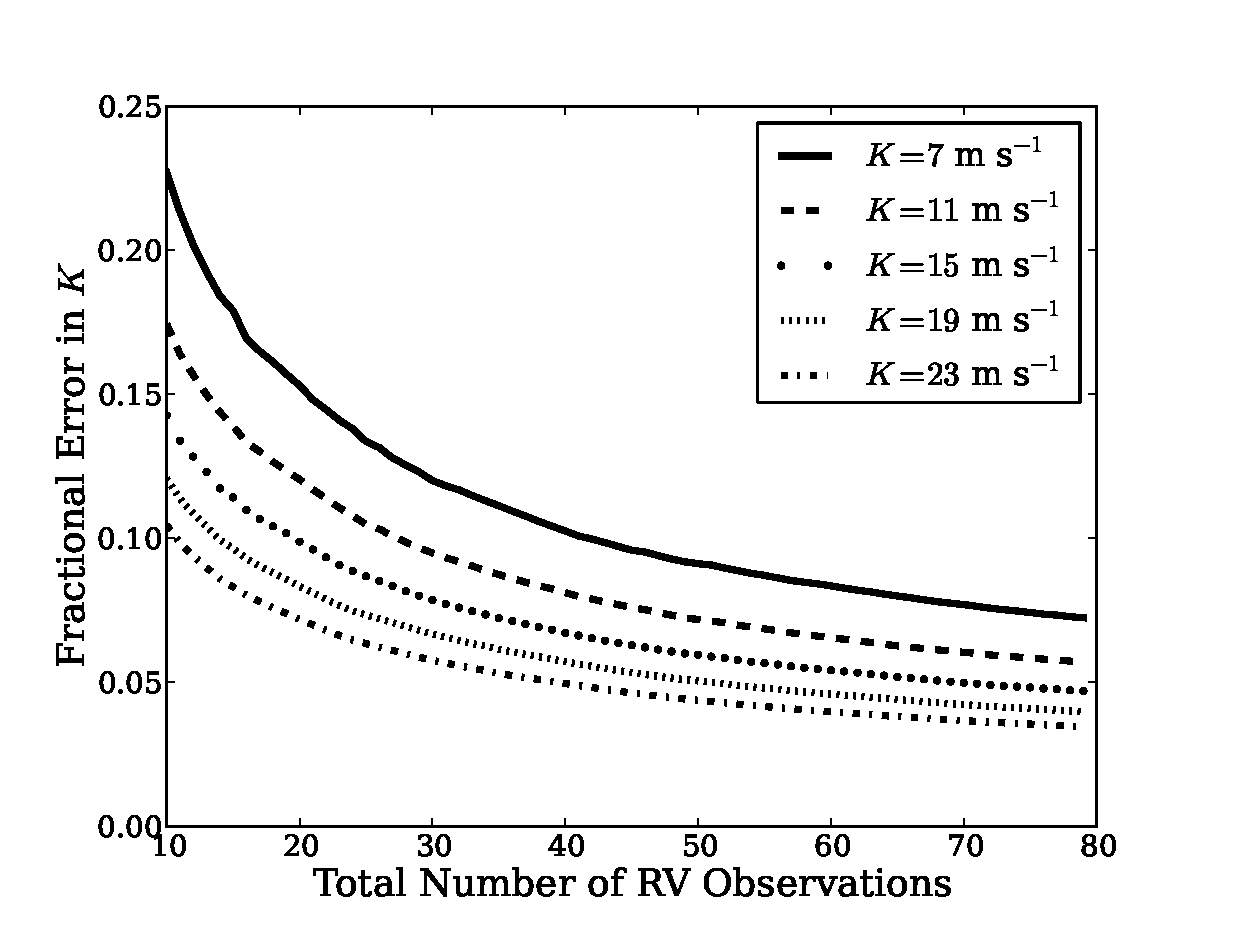
\includegraphics[width=0.75\textwidth]{chapter2/f1.eps}}
\caption[Simulated RV precision as a function of the number of
observations for specified Doppler semiamplitudes]{Derived fractional errors in the Doppler semiamplitude measurement as a function of number of radial velocity observations taken, for various values of $K$, the Doppler semiamplitude. For all observations, the same statistical uncertainties and RV jitter levels are assumed. The jitter level is 3 m/s, a reasonable estimate for all but the youngest dwarf stars. From top to bottom, these curves represent semiamplitudes of $[7, 11, 15, 19, 23]$ m/s. For a system like Kepler-18, where $K \approx 7$ m/s, many more measurements would be required to constrain $K$ to five percent (and thus the stellar mass to 15 percent). However, for a system with either larger planets or a smaller star, this level of precision could be reached with fewer observations.
  }

\label{RVerrors}
\end{figure}



\section{Summary and Discussion}

\label{S:SD}

We present a  method of measuring stellar and planetary masses dynamically by combining TTVs measured from transit light curves and follow-up radial velocity measurements. Our method can be used as an alternative to relying on stellar evolutionary models, which can be poorly constrained for non-solar type stars like M-dwarfs, subgiants, and F stars. By analyzing the Kepler-18 system and confirming our expressions with dynamical simulations of this system, we show the potential of our method.

While we show our method to be viable, especially for low-mass stars, using our method requires a somewhat specific set of circumstances. The system must contain two planets with masses large enough to force a detectable Doppler signal and observable transit timing variations on circular orbits near a first-order commensurability. \kep\ data suggests planets near resonance are common: more than 12 percent of planet systems show evidence for detectable transit timing variations \citep{Ford12a}, and dozens of planets near resonance have been confirmed through TTVs \citep{Steffen13}. Both the TTV and Doppler signals can be measured for super-Earth planets with periods less than 30 days; short-period systems such as these are extremely common \citep{Howard12}. Thus, it is likely that despite the specific requirements needed to use our system, it can be applied to a considerable number of \kep\ planetary systems.

As shown in Equations 14 and 15 of L12, the amplitude of the TTV signal is given such that
\begin{equation}
|V| \sim |V_\textrm{damped}|\bigg(1 + \frac{|Z_\textrm{free}|}{|\Delta|}\bigg),
\end{equation}
with $|V_\textrm{damped}|$ the amplitude of the TTV signal if the system were damped of its free eccentricity. The quantity $Z_\textrm{free}$ is defined such that $Z_\textrm{free} = f z_\textrm{free} + g z^\prime_\textrm{free}$, where $z$ is the complex eccentricity of the planet, $z = e\exp^{i \omega}$. Thus, our method as described will break down unless $|Z_{\textrm{free}}| \ll |\Delta|$. This is a resonable assumption for planets with periods under ten days. In theory, even if a non-negligible amount of free eccentricity remains in the system, a detailed radial velocity orbital solution could be used to calculate $Z_{\textrm{free}}$ and determine the system dynamical masses.

As a projection of the utility of this method, consider KOI 1241, a system containing two planets with periods of 10.5 and 21.4 days orbiting a giant star \citep[$R = 3.14 R_\odot$,][]{Steffen13}. There is evidence that this system has not dissipated all its free eccentricity, meaning it is not optimal for our study. However, with nine quarters of public \kep\ data, we can constrain the TTV signal caused by the larger planet in this system to 8.2 percent. Moreover, with only nine radial velocity observations, we can determine the radial velocity semiamplitude of the larger planet to 5.3 percent. Thus, from our method alone, if a system existed that was nearly identical to KOI 1241 but damped of free eccentricity, by Equations 11-13, we expect we could determine the stellar mass to 29 percent and the mass of the larger planet to within 22 percent. Our method could also be applied to KOI 1241 in the future if enough radial velocity data is collected to determine the magnitude of $Z_\textrm{free}$ for the system. The uncertainties in the TTV signal of KOI 1241 are larger than the uncertainty in the RV semiamplitude. The transit timing errors will decrease as more \kep\ data are released: decreasing the TTV error to five percent without including any additional radial velocity observations will reduce the uncertainty in the stellar mass to 20 percent. Thus our method could provide significant constraints on stellar masses in regimes where stellar atmospheres are less well-understood, such as subgiants and cool stars. For these cases, our method will be able to compliment asteroseismology results as an independent measure on the mass of the star. Moreover, our method can be used to find systems where the analytic stellar mass is substantially different than the Kepler Input Catalog values, which can then be followed up with dynamical modeling, asteroseismology, or high resolution spectroscopy to better characterize the star and orbiting planets.

With present data our technique is only viable as an alternative to stellar modeling in the most exceptional cases. Transit timing variations have been detected to remarkable precision by \textit{Kepler}, but very few KOIs have been followed up with radial velocity measurements. In the cases where RV data exists, only enough measurements were collected to confirm the planetary nature of the system, not to independently measure the planetary masses \citep{Holman10}. Our routine will become more useful for systems in which the RV semiamplitude can be better constrained. Additionally, the constraints provided by our technique can be applied as priors for model-grid interpolations of stellar masses. Thus these model-independent mass measurements can be used to guide and improve model-based stellar mass estimates.

Despite the faintness of the \kep\ planet candidate host stars, there are a few stars that would be ideal candidates for applications of our method. From the collection of Kepler Objects of Interest, we searched for stars hosting at least two transiting planets each with $P < 25$ days. We required at least one planet to be larger than 2 $R_\oplus$ and the planet periods to lie within five percent of a first-order mean-motion resonance. To ensure that all targets were optimized for radial velocity follow-up, we eliminated all targets fainter than $m_{\textrm{Kp}} = 13.0$. After making these cuts, we find 8 candidate systems to which this technique can be applied: KOI 85, 111, 115, 117, 244, 304, 1241 and 1930. As stated earlier in this section, KOI 1241 is not an ideal target because it has not been fully damped of its primordial eccentricity and there is not enough radial velocity information to uniquely determine the eccentricity of both planets. Of the remaining 7 systems, the CPS team has collected more than 10 radial velocity measurements only on one, KOI 244. Additional radial velocity measurements of any or all of the above systems would enable further validation of our procedure as well as additional constraints on the masses of each of the stars and their planets. Moreover, next-generation planet finding missions, such as TESS \citep{Brown08} and PLATO \citep{Catala10} will target bright stars, making detailed radial velocity follow-up observations of systems exhibiting transit timing variations a much more practical possibility. 

{\footnotesize
\begin{longtable}{lcccc} 
\hline
KOI & n & $t_n$ & TTV$_n$ & $\sigma_n$ \\
    &   & (BJD-2454900) & (d) & (d) \\
\hline
137.01 & 0 & 198.3142 & -0.0006 &  0.0012 \\
137.01 & 1 & 205.9557 &  0.0002 &  0.0013 \\
137.01 & 2 & 213.5973 &  0.0019 &  0.0018 \\
137.01 & 3 & 221.2389 &  0.0017 &  0.0010 \\
137.01 & 4 & 228.8804 &  0.0021 &  0.0017 \\
137.01 & 5 & 236.5220 &  0.0014 &  0.0015 \\
137.01 & 6 & 244.1636 &  0.0031 &  0.0011 \\
137.01 & 7 & 251.8052 &  0.0030 &  0.0011 \\
137.01 & 8 & 259.4467 &  0.0037 &  0.0012 \\
137.01 & 9 & 267.0883 &  0.0050 &  0.0012 \\
137.01 & 10 & 274.7299 &  0.0041 &  0.0012 \\
137.01 & 11 & 282.3714 &  0.0037 &  0.0018 \\
137.01 & 12 & 290.0130 &  0.0035 &  0.0018 \\
137.01 & 13 & 297.6546 &  0.0028 &  0.0012 \\
137.01 & 14 & 305.2961 &  0.0034 &  0.0011 \\
137.01 & 15 & 312.9377 &  0.0026 &  0.0011 \\
137.01 & 16 & 320.5793 &  0.0013 &  0.0011 \\
137.01 & 17 & 328.2209 &  0.0018 &  0.0012 \\
137.01 & 18 & 335.8624 &  0.0008 &  0.0015 \\
137.01 & 20 & 351.1456 &  0.0001 &  0.0011 \\
137.01 & 21 & 358.7871 & -0.0005 &  0.0012 \\
137.01 & 22 & 366.4287 & -0.0027 &  0.0014 \\
137.01 & 23 & 374.0703 & -0.0033 &  0.0014 \\
137.01 & 24 & 381.7119 & -0.0024 &  0.0011 \\
137.01 & 25 & 389.3534 & -0.0025 &  0.0011 \\
137.01 & 26 & 396.9950 & -0.0033 &  0.0011 \\
137.01 & 27 & 404.6366 & -0.0036 &  0.0013 \\
137.01 & 28 & 412.2781 & -0.0046 &  0.0012 \\
137.01 & 29 & 419.9197 & -0.0037 &  0.0011 \\
137.01 & 30 & 427.5613 & -0.0038 &  0.0015 \\
137.01 & 31 & 435.2028 & -0.0039 &  0.0013 \\
137.01 & 32 & 442.8444 & -0.0019 &  0.0012 \\
137.01 & 33 & 450.4860 & -0.0013 &  0.0011 \\
137.01 & 34 & 458.1276 & -0.0017 &  0.0010 \\
137.01 & 35 & 465.7691 & -0.0008 &  0.0015 \\
137.01 & 36 & 473.4107 &  0.0005 &  0.0013 \\
137.01 & 37 & 481.0523 &  0.0016 &  0.0011 \\
137.01 & 38 & 488.6938 &  0.0026 &  0.0014 \\
137.01 & 39 & 496.3354 &  0.0027 &  0.0015 \\
137.01 & 40 & 503.9770 &  0.0030 &  0.0014 \\
137.01 & 41 & 511.6186 &  0.0038 &  0.0011 \\
137.01 & 42 & 519.2601 &  0.0032 &  0.0013 \\
137.01 & 43 & 526.9017 &  0.0052 &  0.0013 \\
137.01 & 44 & 534.5433 &  0.0055 &  0.0013 \\
137.01 & 45 & 542.1848 &  0.0034 &  0.0010 \\
137.01 & 46 & 549.8264 &  0.0025 &  0.0014 \\
137.01 & 47 & 557.4680 &  0.0049 &  0.0021 \\
137.01 & 48 & 565.1095 &  0.0035 &  0.0011 \\
137.01 & 49 & 572.7511 &  0.0030 &  0.0012 \\
137.01 & 50 & 580.3927 &  0.0017 &  0.0010 \\
137.01 & 51 & 588.0343 &  0.0034 &  0.0016 \\
137.01 & 52 & 595.6758 &  0.0013 &  0.0011 \\
137.01 & 54 & 610.9590 & -0.0006 &  0.0012 \\
137.01 & 55 & 618.6005 & -0.0019 &  0.0012 \\
137.01 & 56 & 626.2421 & -0.0015 &  0.0016 \\
137.01 & 57 & 633.8837 & -0.0026 &  0.0012 \\
137.01 & 58 & 641.5253 & -0.0016 &  0.0012 \\
137.01 & 61 & 664.4500 & -0.0046 &  0.0014 \\
137.01 & 62 & 672.0915 & -0.0028 &  0.0012 \\
137.01 & 63 & 679.7331 & -0.0042 &  0.0012 \\
137.01 & 65 & 695.0162 & -0.0032 &  0.0011 \\
137.01 & 66 & 702.6578 & -0.0025 &  0.0013 \\
137.01 & 67 & 710.2994 & -0.0029 &  0.0012 \\
137.01 & 68 & 717.9410 & -0.0029 &  0.0011 \\
137.01 & 69 & 725.5825 & -0.0004 &  0.0013 \\
137.01 & 71 & 740.8657 &  0.0006 &  0.0013 \\
137.01 & 72 & 748.5072 &  0.0006 &  0.0014 \\
137.01 & 73 & 756.1488 &  0.0014 &  0.0011 \\
137.01 & 74 & 763.7904 &  0.0049 &  0.0017 \\
137.01 & 75 & 771.4320 &  0.0011 &  0.0016 \\
137.01 & 76 & 779.0735 &  0.0033 &  0.0012 \\
137.01 & 77 & 786.7151 &  0.0021 &  0.0011 \\
137.01 & 78 & 794.3567 &  0.0031 &  0.0012 \\
137.01 & 79 & 801.9982 &  0.0039 &  0.0012 \\
137.01 & 80 & 809.6398 &  0.0029 &  0.0014 \\
137.01 & 81 & 817.2814 &  0.0038 &  0.0011 \\
137.01 & 82 & 824.9229 &  0.0016 &  0.0012 \\
137.02 & 0 & 194.8832 &  0.0000 &  0.0010 \\
137.02 & 1 & 209.7421 & -0.0012 &  0.0011 \\
137.02 & 2 & 224.6011 & -0.0025 &  0.0010 \\
137.02 & 3 & 239.4600 & -0.0037 &  0.0010 \\
137.02 & 4 & 254.3189 & -0.0029 &  0.0010 \\
137.02 & 6 & 284.0368 & -0.0032 &  0.0011 \\
137.02 & 7 & 298.8958 & -0.0040 &  0.0011 \\
137.02 & 8 & 313.7547 & -0.0013 &  0.0010 \\
137.02 & 9 & 328.6136 & -0.0023 &  0.0023 \\
137.02 & 10 & 343.4726 & -0.0005 &  0.0011 \\
137.02 & 11 & 358.3315 &  0.0008 &  0.0009 \\
137.02 & 12 & 373.1905 &  0.0017 &  0.0012 \\
137.02 & 13 & 388.0494 &  0.0036 &  0.0010 \\
137.02 & 14 & 402.9083 &  0.0029 &  0.0011 \\
137.02 & 15 & 417.7673 &  0.0020 &  0.0010 \\
137.02 & 16 & 432.6262 &  0.0008 &  0.0012 \\
137.02 & 17 & 447.4852 &  0.0008 &  0.0011 \\
137.02 & 18 & 462.3441 &  0.0008 &  0.0011 \\
137.02 & 19 & 477.2030 & -0.0001 &  0.0011 \\
137.02 & 20 & 492.0620 &  0.0002 &  0.0010 \\
137.02 & 21 & 506.9209 & -0.0023 &  0.0011 \\
137.02 & 22 & 521.7799 & -0.0024 &  0.0010 \\
137.02 & 23 & 536.6388 & -0.0038 &  0.0010 \\
137.02 & 24 & 551.4977 & -0.0035 &  0.0010 \\
137.02 & 25 & 566.3567 & -0.0033 &  0.0011 \\
137.02 & 26 & 581.2156 & -0.0033 &  0.0010 \\
137.02 & 27 & 596.0746 & -0.0013 &  0.0015 \\
137.02 & 29 & 625.7924 &  0.0020 &  0.0010 \\
137.02 & 31 & 655.5103 &  0.0032 &  0.0014 \\
137.02 & 32 & 670.3693 &  0.0015 &  0.0011 \\
137.02 & 33 & 685.2282 &  0.0026 &  0.0009 \\
137.02 & 34 & 700.0871 & -0.0011 &  0.0011 \\
137.02 & 35 & 714.9461 &  0.0008 &  0.0010 \\
137.02 & 36 & 729.8050 & -0.0019 &  0.0010 \\
137.02 & 37 & 744.6640 & -0.0012 &  0.0011 \\
137.02 & 38 & 759.5229 & -0.0027 &  0.0011 \\
137.02 & 39 & 774.3818 & -0.0030 &  0.0012 \\
137.02 & 40 & 789.2408 & -0.0034 &  0.0010 \\
137.02 & 41 & 804.0997 & -0.0052 &  0.0010 \\
137.02 & 42 & 818.9587 &  0.0003 &  0.0013 \\
\hline
\caption{Transit times for \kep\ transiting planet candidates
in the KOI-137 system}
\label{TTTable}
\end{longtable}
}




\chapter{The Occurrence Rate of Giant Planets around M Dwarfs}
\label{chap:trends}

In this chapter I develop a method to determine the occurrence
rate of giant planets in wide orbits around their host stars.
These planets are large enough to cause a slow drift, or trend, in 
the RV of their host star, but too distant from their star to
observe the full orbit on a reasonable timescale.
Such a trend could be caused by a planet, or a star on a much
wider orbit. As stars would be easily observable with high-contrast
direct imaging, the existence of a trend combined with an AO 
non-detection suggests the presence of a planet is likely.
The definitive presence of any single planet can not be 
determined, but by analyzing a population of these systems their
bulk occurrence can be measured.
This chapter was originally published as ``The TRENDS High-contrast Imaging Survey. IV. The Occurrence Rate of Giant Planets around M Dwarfs,'' ApJ, 781, 28 (2014) by BTM, Justin Crepp, John Johnson,
Andrew Howard, and Geoff Marcy. 


\section{Introduction}

Over the past twenty years, numerous planets have been detected by several different techniques, permitting the first estimates of the occurrence rate of planets orbiting stars in the solar neighborhood \citep[e.g.][]{Johnson10b, Howard10b, Gould10, Vigan12}. As successful as these detection methods have been, each is sensitive only to a relatively narrow range of parameter space. For example, radial velocity (RV) studies are most sensitive to massive planets with orbital periods shorter than the time baseline of observations. %For example, 
% \citet{Wright12} calculate that $1.20\% \pm 0.38\%$ of FGK stars host a ``hot Jupiter'' with mass larger than $m \sin i > 0.1 M_J$ and period shorter than 10 days. By analyzing stars with longer period RV signals,
\citet{Johnson10b} find that $3.4^{+2.2}_{-0.9}\%$ of M dwarfs have a Saturn-mass or larger planet within 2.5 AU. Beyond a few AU, RV searches are incomplete as the time required for a planet to complete one orbit is longer than the typical observing baseline. Some studies have attempted to extrapolate beyond this boundary. For instance, \citet{Cumming08} fit the observed RV planet population to a power law in planet mass and period and find that $18\% \pm 1\%$ of FGK stars host a Saturn-mass or larger planet within 20 AU. Recently, targeted RV surveys of M-dwarfs have suggested the giant planet occurrence rate is significantly smaller for these diminutive stars. \citet{Bonfils13} suggest fewer than $1\%$ of M-dwarfs host a Saturn-mass or larger planet with an orbital period $1 < P < 10$ days, and $2^{+3}_{-1}\%$ host giant planets with orbital periods between 10 and 100 days.

Transit studies suffer from similar detection biases. Since a planet transits only once each orbit, several orbits must be observed to definitively confirm a planet so characterization is limited to planets with periods shorter than a fraction of the observing baseline \citep{Gaudi05}. Additionally, the probability of a planet transiting its host star decreases with increasing orbital period \citep{Winn11}, such that hundreds of thousands of stars must be monitored in order to study the planet population at $a \approx 1$ AU \citep{Borucki84}. Nevertheless, the success of the \textit{Kepler} mission \citep{Borucki10, Koch10} has allowed for statistical analyses of transiting planets to be undertaken. For example, \citet{Morton14} analyze M dwarfs included in the 2012 list of announced Kepler Objects of Interest \citep[KOIs,][]{Batalha13}. By correcting for false positives (detections when no transiting planet exists), false negatives (nondetections when a transiting planet is present) and geometric effects (nondetections of nontransiting planets), they estimate an occurrence rate of $1.5$ planets with periods less than 90 days and radii larger than $0.5R_\oplus$ per M dwarf star. The occurrence rate found by these authors is slightly higher than previous analyses which measure rates of approximately one planet per star \citep{Youdin11, Mann12, Swift13, Dressing13}.

Neither RV nor transit searches are yet conducive to the discovery and characterization of planets well beyond the ``snow line,'' where water exists as ice. Instead, high contrast direct imaging techniques can be a powerful tool for detecting young planetary companions in this domain. The first direct imaging planet discoveries are securely in hand, including four companions to HR\,8799 \citep{Marois08, Marois10} and one each around $\beta$ Pictoris \citep{Lagrange09}, and Gl\,504 \citep{Kuzuhara13}\footnote{Companions detected around Fomalhaut \citep{Kalas08, Currie12}, HD 95086 \citep{Rameau13}, and LaCa15 \citep{Kraus12} are also good candidates to be directly imaged planets, but their true nature is somewhat ambiguous.}. Recent studies using these techniques have calculated an occurrence rate around A stars of $8.7^{+10.1}_{-2.8}\%$ at $1\sigma$ confidence for planets larger than $3 M_J$ and separations between 5 and $320 \textrm{ AU}$ \citep{Vigan12}. Imaging studies have been most effective around high mass stars. \citep{Crepp11, Carson13}. Nondetections around lower-mass stars have been used to place upper limits on the frequency of giant planets. For example, \citet{Nielsen10} rule out the presence of giant planets orbiting FGKM stars beyond 65 AU with $95\%$ confidence. High contrast imaging, while powerful, only provides a measure of the relative brightness of a companion. To estimate the companion's mass, the age of the star must be known and planetary thermal evolution models must be applied to estimate the temperature (and brightness) of the companion \citep{Chabrier00, Baraffe03}. Moreover, direct imaging is currently only sensitive to massive planets; the HR8799 planets and $\beta$ Pic b are believed to have masses $m > 5 M_J$. RV and transit studies suggest such ``super-Jupiters'' are rare compared to Jovian-mass and smaller objects at smaller separations \citep{Howard10b, Howard12}.

The gravitational microlensing technique is also effective for finding giant planets in wide orbits and does not rely on planetary evolution models. Using this technique, planets can be detected by observing perturbations to the photometric gravitational microlensing signal when a planet and its host pass in front of a more distant star. Since $70-75\%$ of stars in the galaxy are M-dwarfs, most lenses have mass $M < 0.5 M_\odot$. Microlensing searches thus provide a measure of planet occurrence around low mass stars. Microlensing studies are sensitive to planets near the Einstein ring, $R_E \sim 3.5 \mbox{AU} (M/M_\odot)^{1/2}$, a much wider separation than RV and transit searches \citet{Gould10}. \citet{Cassan12} find microlensing searches are most sensitive to planets at a projected separation in the range $[s_{\textrm{max}}^{-1}R_E, s_{\textrm{max}}R_E]$, where $s_{\textrm{max}} \sim (q/10^{-4.3})^{1/3}$ and $q$ is the mass ratio between a companion and the host star. These authors find a planet occurrence rate that can be parameterized by a double power-law function, in mass ratio $q$ and separation $s$, such that
\begin{equation}
\frac{d^2N}{d\log q d \log s} = 10^{-0.62 \pm 0.22} \bigg(\frac{q}{5 \times 10^{-4}}\bigg)^{-0.73 \pm 0.17} \mbox{dex}^{-2}.
\label{microlensingresults}
\end{equation}
The normalization constant is equivalent to $0.24^{+0.16}_{-0.10}$. These results are calculated under the assumption that planets are distributed uniformly in $\log s$, as is the case for binary stars \citep{Opik24}. Additionally, \citet{Sumi10} find a power-law slope in mass such that $dN/ d\log q \propto q^{-0.68 \pm 0.20}$ for Neptune-sized planets, but do not attempt to quantify a normalization factor. 

As microlensing studies focus on distant M-dwarfs ($d > 1$ kpc) in the direction of the galactic bulge \citep{Gaudi02}, these stars can be difficult to characterize accurately due to crowding. Stellar masses and metallicities are often estimated without being measured spectroscopically. If these host stars have different masses than assumed, it would affect the results of planet occurrence rate studies by microlensing groups as microlensing results do not account for correlations between stellar and planet properties. Additionally, as microlensing searches are most sensitive near $r = R_E$, beyond approximately 10 AU the lensing signal becomes very weak, and differentiating distant planets from unbound, ``free-floating'' planets becomes difficult \citep{Sumi11}.

RV and microlensing studies probe different regions around a star, and extrapolations between the two domains suggest a possible discrepancy. \citet{Cassan12} estimate a total giant planet occurrence rate significantly lower than the \citet{Cumming08} RV result.
% studied the statistics of the Keck/HIRES Doppler survey and found that $18 \pm 1 \%$ of FGK dwarfs have a planet at least as massive as Saturn within 20 AU, lower than the predictions offered by microlensing results. 
Derived power-law distributions in mass may also be different for planets found by each method: \citet{Cumming08} find a distribution such that $dN/d \log m \propto m^{-0.31 \pm 0.20}$ from RV-detected planets, while \citet{Cassan12} find a distribution such that $dN/ d\log q \propto q^{-0.73 \pm 0.17}$. Since microlensing studies target M-dwarfs, which are confined to a narrow mass range, we can approximate $q = m/M$ as $m$. In this case, the microlensing result and RV result differ by $1.6 \sigma$.  Since giant planet occurrence decreases with decreasing stellar mass and metallicity \citep{Johnson10a}, the expected giant planet occurrence rate around M dwarfs would be smaller than that for FGK stars. Therefore, it is necessary to compare the microlensing planet population not to a population of FGK stars, but instead to a study of RV detected planets around M-dwarfs.

Historically, RV observations have been used to detect and characterize planets once they complete a full orbit, limiting studies to planets with periods shorter than the observing time baseline. In this paradigm, potentially useful information is overlooked. Wide companions are not completely undetectable: instead they can be identified by the presence of long-term RV accelerations (linear ``trends'')  which can be used to infer the existence of a companion in a more distant orbit \citep{Liu02, Crepp12a}. However, a linear acceleration does not provide unique information about the mass and period of the companion: the same trend could be caused by a Jupiter-mass planet at 5 AU or a $100 M_J$ M-dwarf at 25 AU. This degeneracy can be broken by adaptive optics (AO) imaging. Low-mass binary companions to nearby M-dwarfs can be easily imaged by modern AO systems \citep{Lloyd02, Siegler03}. Such detections form the basis for the TRENDS High-Contrast Imaging Survey, which to date has detected four M-dwarfs and one white dwarf companion to higher mass stars\citep{Crepp12b, Crepp13a, Crepp13b}.

In this work, we combine RV and AO observations of nearby cool stars to estimate the frequency of giant planets in wide orbits around M-dwarfs. From a sample of 111 M-dwarfs observed with a median Doppler RV baseline of 11.8 years, we identify 4 systems with long-term RV accelerations but no known companions and target these stars with AO imaging in an attempt to detect stellar-mass companions. We discuss these observations and our methodology in \textsection\ref{SO}. Given an observed RV trend or lack thereof, we determine with high statistical confidence if a giant planet exists around each star. We analyze the effects of false positive and false negative detections of RV accelerations in our sample in \textsection\ref{Stats}. In \textsection\ref{Results} we estimate the occurrence rate of giant planets around M-dwarfs and compare the measure to results from other techniques. We summarize and conclude in \textsection\ref{SC}, and 
provide notes about individual targets in \textsection 6.
In \textsection 7, we include a brief note about magnetic activity.

 This study represents the first measurement of the planet population in the range 0--20 AU. While we rely on brown dwarf cooling models, our study does not make use of theoretical planetary evolution models, unlike other AO studies of planetary systems.

\section{Sample and Observations}
\label{SO}
\subsection{Target Selection}
\label{TS}

Since 1997, the California Planet Search (CPS) collaboration has undertaken a comprehensive Doppler search for extrasolar planets at the Keck Observatory \citep[e.g. ][]{Howard10}. Using Keck/HIRES \citep{Vogt94}, the CPS program monitors over 2000 stars, most selected to be chromospherically quiet, single, and bright. Included in this sample is a collection of M-dwarfs from the Gliese and Hipparcos catalogs brighter than $V = 11.5$ and lacking known stellar companions within 2 arcseconds \citep{Rauscher06}. This sample was later extended to $V = 13.5$ and currently includes 131 M-dwarfs within 16 pc of the Sun, where we define the M spectral class as targets with $B-V > 1.44$.

To develop the sample used here, we first remove from this set 16 stars with a known, nearby stellar binary companion. We define ``nearby'' as a separation small enough that a test particle orbit with semimajor axis $\geq 30$ AU would be unstable, following the instability criterion of \citet{Holman99}. This criterion depends on the unknown eccentricity of the binary pair, as perturbative effects are maximized at periapsis. We take $e=0.5$ as a typical value and find the onset of instability occurs for binary stars with $a \sim 250$ AU. Planets can still form in these more compact binary systems \citep[e.g. Gl667C; ][]{Anglada-Escude12b} but at such small separations protoplanetary disk formation and planet evolution would be affected significantly by the presence of stellar companions. This selection thus allows us to study a class of planets that likely followed similar evolutionary processes. Moreover, the detection of an acceleration around these stars is ambiguous, as it could be caused by the binary star, a planetary-mass companion, or both together.

After making the above selection we are left with 111 RV targets, all of which have at least 8 radial velocity observations and a time baseline longer than 2.9 years. The median number of observations is 29 over a median time baseline of 11.8 years. The stars have spectral types from M0 to M5.5 and masses in the range $0.64M_\odot - 0.10M_\odot$. Stellar masses are estimated using the empirical relation between mass and absolute K-band magnitude, $M_K$, described by \citet{Delfosse00}. We take $10\%$ as a typical uncertainty in the stellar mass, in line with previous estimates \citep{Bean06}. $K$-band apparent magnitudes are measured using apparent magnitudes from the 2MASS point-source catalog \citep{Cutri03}. The majority of our parallaxes are taken from an analysis of \textit{Hipparcos} data \citep{vanLeeuwen07}. Some of our stars were not observed by Hipparcos, while others have had their distances updated more recently. In these cases, we apply the distances listed in the SIMBAD astronomical database (Table \ref{T1}). For example, for Gl\,317 we use the parallax found by \citet{Anglada-Escude12a}; their derived mass and metallicity are consistent with our estimated values. In all cases, stellar metallicities are estimated by measuring the offset between the star's position in the \{$V-K_s, M_{K_S}$\} plane from a calibrated main sequence following the method of \citet{Neves12}. We take 0.17 dex as a typical uncertainty in the stellar metallicity, representative of the scatter between this photometric method and spectroscopic measures of stellar metallicity. Stellar parameters for these targets are listed in Table \ref{T1} and observational parameters are listed in Table \ref{T1b}. The distribution of RV observational parameters are shown in Figure \ref{Hists}. Spectral types are estimated by comparing the spectrum collected with HIRES to other spectra collected with this same instrument. RV observations for a representative sample of six ``typical'' stars are shown in Figure \ref{RVfig}. 

\begin{figure}[htbp]
\centerline{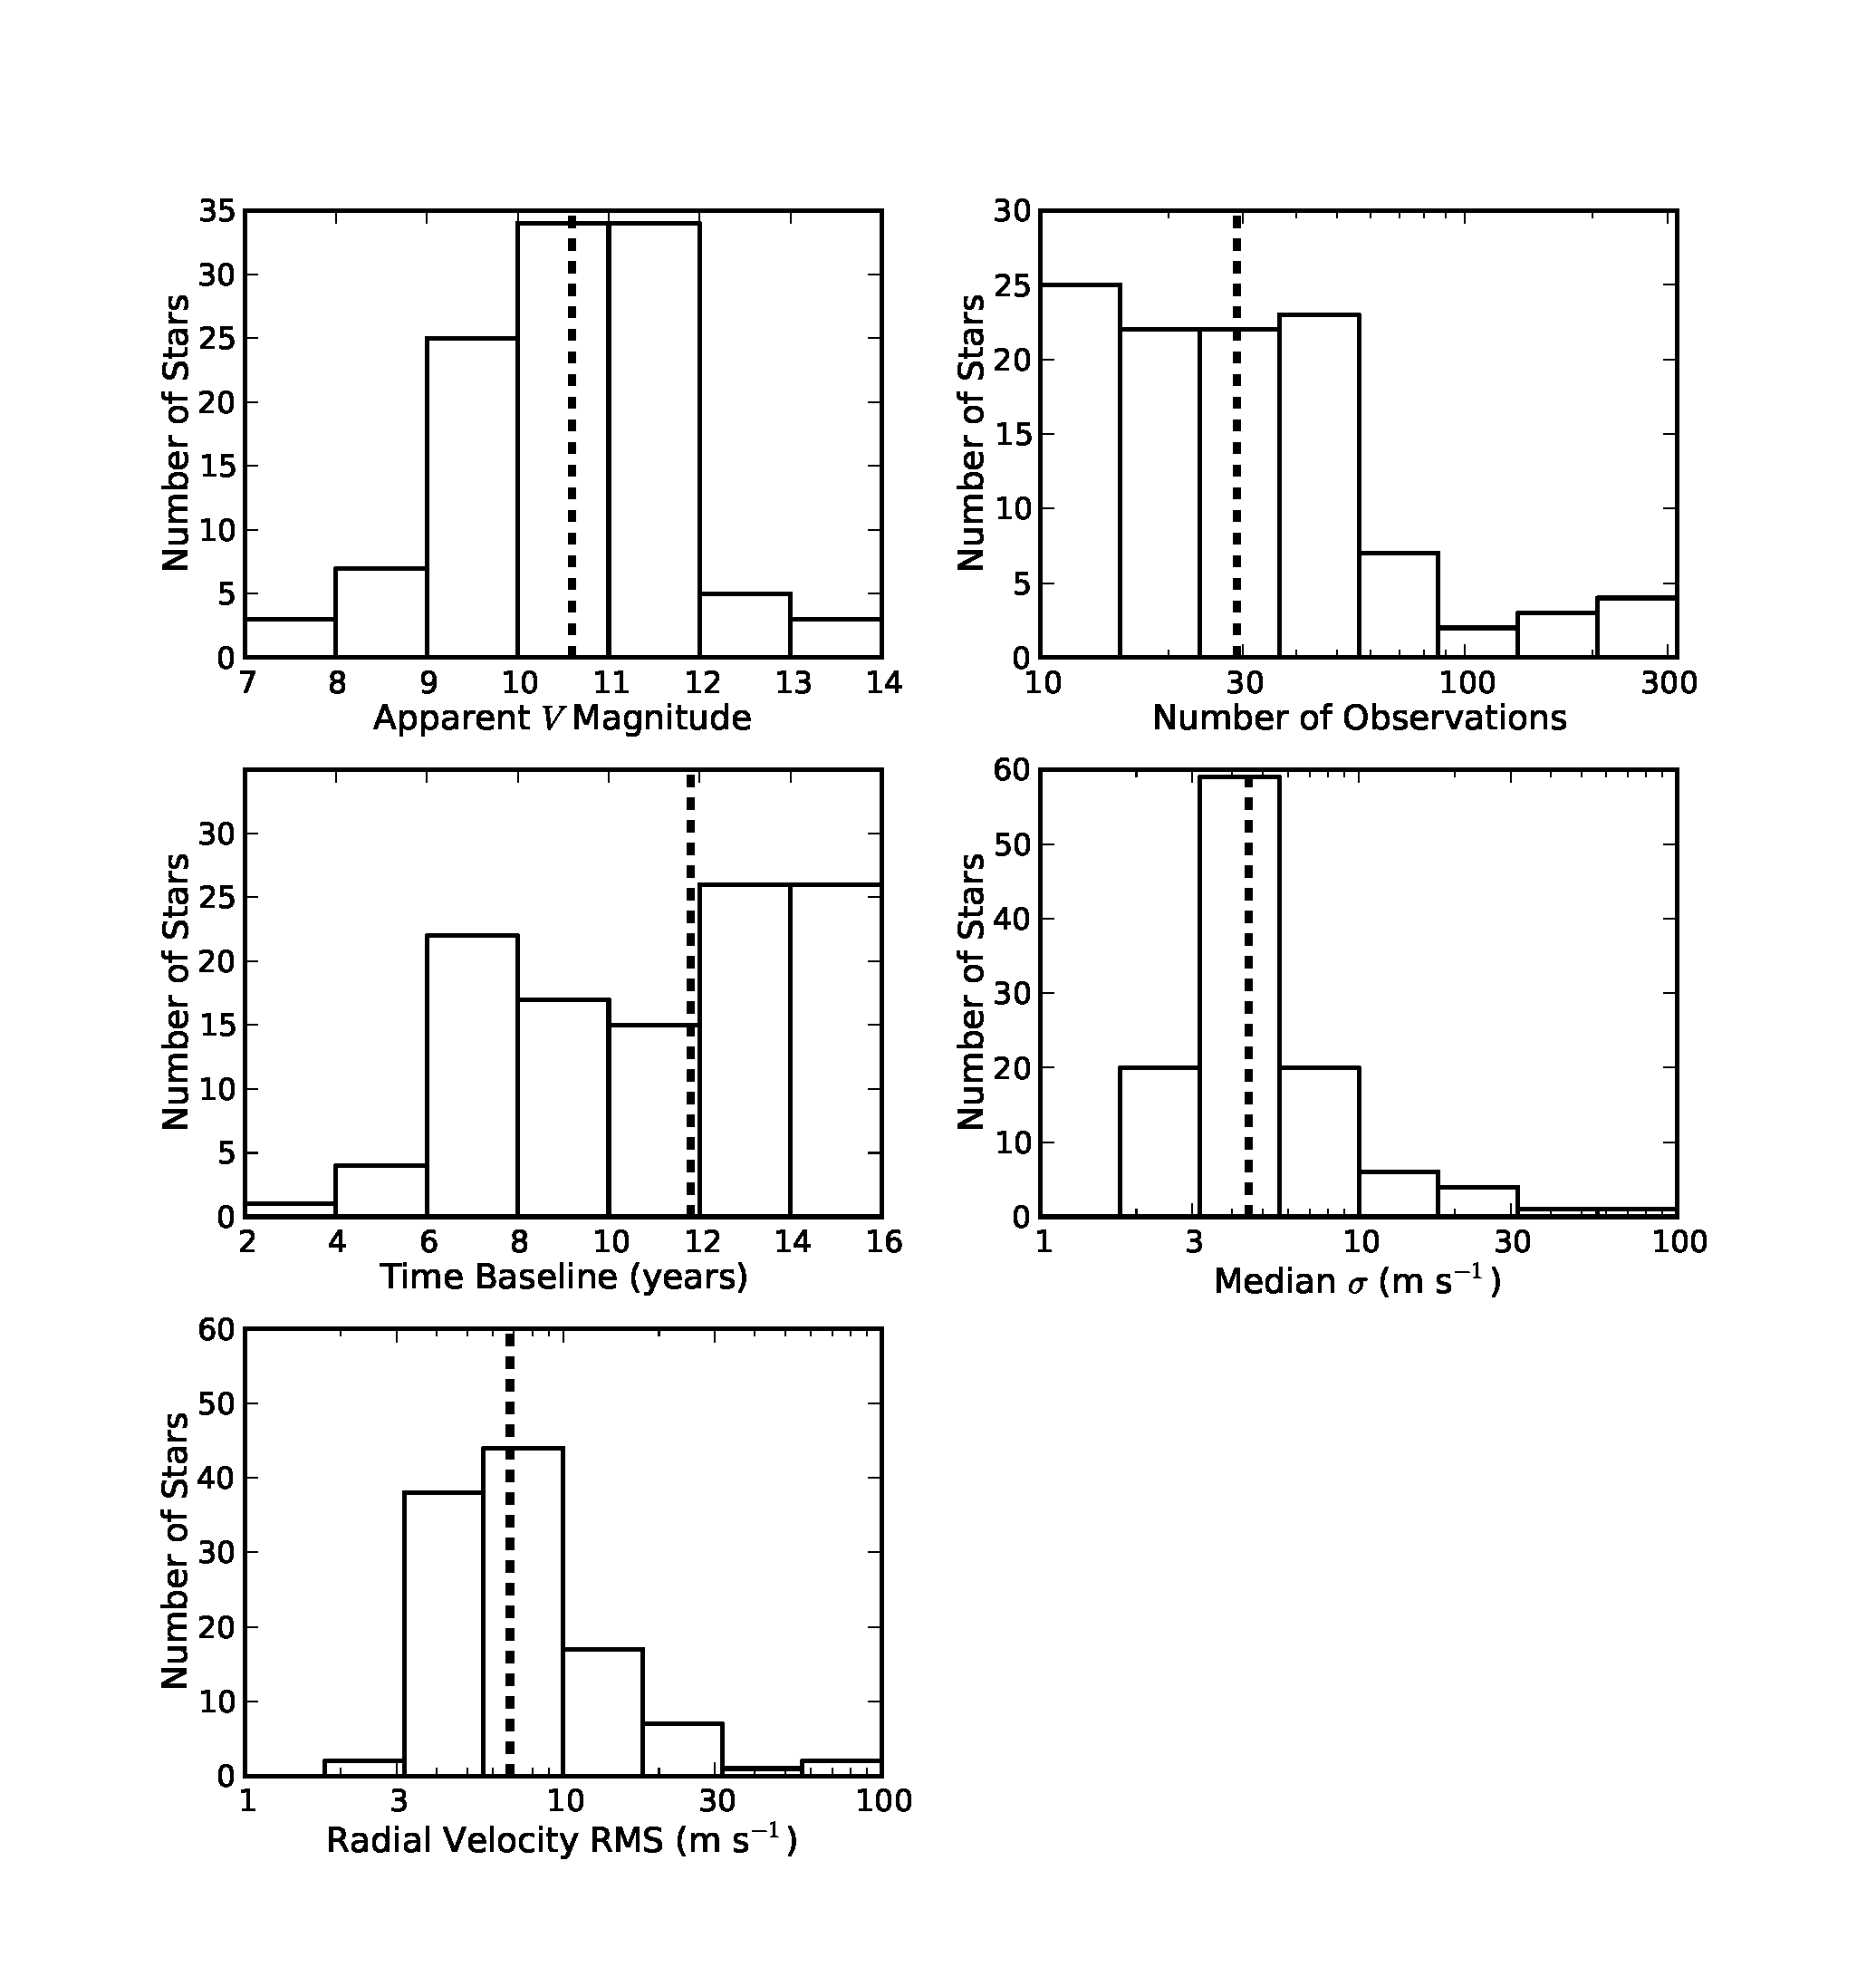
\includegraphics[width=1.0\textwidth]{chapter3/f1.eps}}
\caption[Summary statistics of RV observations]{Distributions of the RV observational parameters. Dashed lines represent the median values for each parameter. The median target brightness is $V = 10.6$, and the median target has been observed 29 times over 11.8 years. The median measurement uncertainty $\sigma$, defined as the sum in quadrature of rotational jitter and statistical uncertainty (Eq. \ref{sigmaeq}) is 4.5 m s$^{-1}$. Specific parameters for each individual system are shown in Table \ref{T1}.
  }
\label{Hists}
\end{figure}


\begin{figure}[htbp]
\centerline{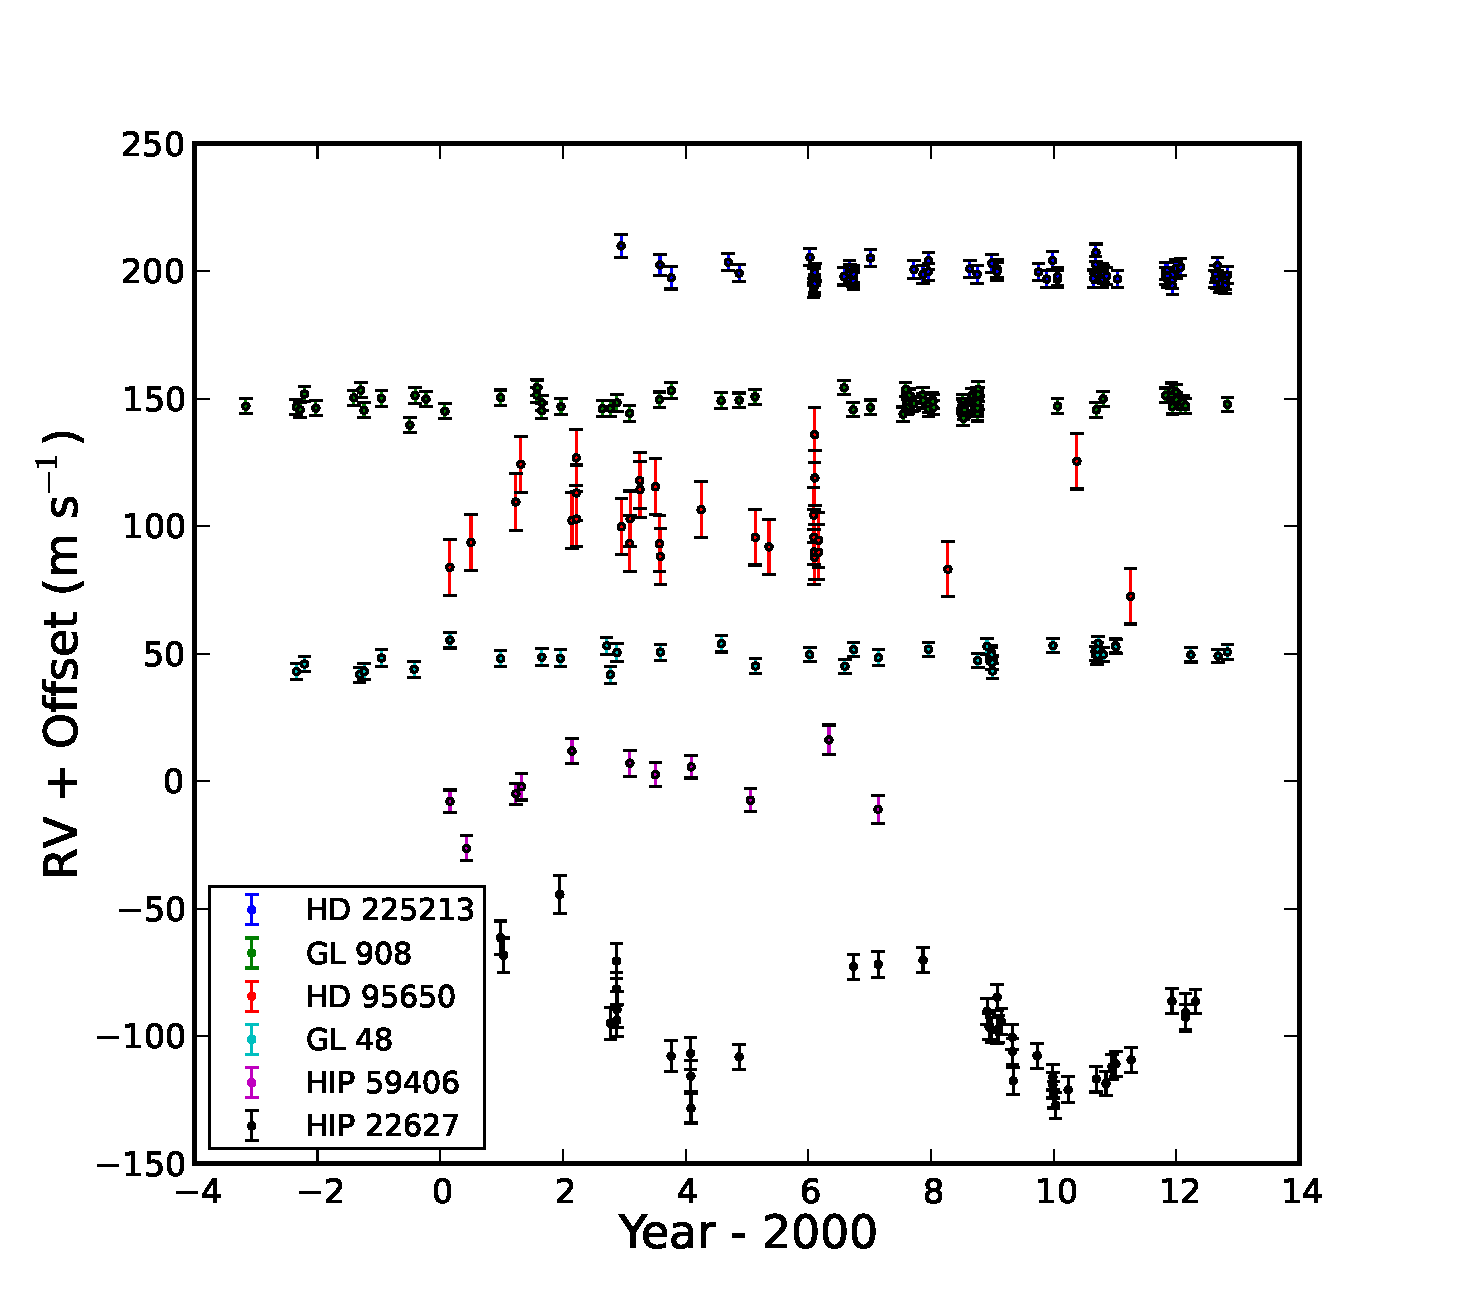
\includegraphics[width=0.75\textwidth]{chapter3/f2.eps}}
\caption[RV measurements for a representative sample of six example stars]{RV measurements for a representative sample of six example stars. The stars are arranged such that the brightest star is at the top of the plot. The individual stars vary considerably with respect to observing baselines, measurement uncertainty, and number of observations. Of these stars, HIP\,59406 has a wide binary companion, while HIP\,22627 has both a known inner planet and long-term RV acceleration.
  }
\label{RVfig}
\end{figure}

\subsection{Detecting Accelerations from Radial Velocities}
\label{RVs}

The detection of a long-term RV acceleration is facilitated by having many observations over a long time baseline to increase signal, but complicated by astrophysical ``jitter'' caused by rotational modulation of surface inhomogeneties. To determine the masses and semimajor axes to which we are sensitive to planetary companions, we inject a series of artificial companions into orbit around the stars in our sample. We define a logarithmically spaced grid of companion masses and semimajor axes spanning the range $0.75 M_J < m < 100 M_J$ and $3 \textrm{AU} < a < 30 \textrm{AU}$, such as the one shown in Figure \ref{Detectability}. At each point, we inject 500 planets and randomly assign each of the remaining orbital elements. The longitude of ascending node $\Omega$, time of periapsis $t_p$, and argument of periapsis $\omega$ are drawn from a uniform distribution, while the inclination is drawn from a distribution $dn/di = \sin i$ and the eccentricity from a distribution such that $dn/de$ follows a beta distribution with $a = 1.12$ and $b = 3.09$, which well-replicates the distribution of observed eccentricities for RV planets with orbits longer than 382 days \citep{Kipping13}. We then numerically integrate these orbits forward in time over our true observing baseline. 



At the epochs each star was observed by CPS, we calculate the expected radial velocity signal caused by our injected planet. Each velocity is perturbed from the true expected Keplerian velocity by a normal variate with zero mean and standard deviation $\sigma$ representative of the total expected noise:
\begin{equation}
\sigma = \sqrt{\sigma_\gamma^2 + \sigma^2_\textrm{jitter}}.
\label{sigmaeq}
\end{equation}
Here, $\sigma_\gamma$ is the photon noise, estimated for each individual observation by randomly selecting a single measurement of the measured Poisson photon noise from a true observation of the star. To account for the effects of jitter, we follow the method of \citet{Isaacson10}, who develop an empirical relation between the level of stellar jitter, a star's $S_{\textrm HK}$ value, and its $B-V$ color. $S_{\textrm HK}$ is defined as the ratio of the flux in the Ca II line cores to flux in the surrounding continuum. We compare the $S_{HK}$ value observed by CPS to that expected from the star's $B-V$ color, which provides an estimate of $\sigma_\textrm{jitter}$. This value is added in quadrature to the photon noise to estimate a total observational uncertainty, $\sigma$. Typical observations carry a photon noise of $2-4$ m s$^{-1}$ and jitter values are typically $3-5$ m s$^{-1}$ for a total $\sigma$ value of $3-6$ m s$^{-1}$ for the majority of stars. Median $\sigma$ values for each star are listed in Table 2.

Once all observations are accounted for, we search for evidence of our injected planetary companion, manifested as an acceleration in the RV data. Here, we define the existence of a trend using the Bayesian Information Criterion \citep[BIC;][]{Schwarz78, Bowler10, Campo11, Stevenson12}, which prefers simple, well-fitting models subject to 
\begin{equation}
\textrm{BIC} \equiv -2 \ln \mathcal{L} + k \ln N,
\label{EqBIC}
\end{equation}  
where $\mathcal{L}$ is the maximum likelihood for a model with $k$ free parameters and $N$ observations. The BIC thus favors models that fit the underlying data well, but penalizes increasingly complex models. For a more complex model to be preferred by the BIC, it must improve the fit by an amount greater than $k \ln N$ to overcome the penalty term.

\citet{Kass95} claim a difference between BIC values provides a bounded approximation of twice the logarithm of the Bayes factor. A change in BIC value of ten or more (corresponding to a Bayes factor of approximately 0.01) suggests strong evidence for an association between two parameters. If the BIC value decreases by more than 10 when considering a model with a linear acceleration over a model with only an offset, a planet is considered to be detected. Otherwise, the system is considered a non-detection. We find that the $\Delta$BIC value chosen here is consistent with by-eye inspection of our data in a visual search for RV accelerations. In both cases, we allow for a linear offset in the RV data in August, 2004, corresponding to an upgrade of the HIRES CCD detector \citep{Wright11}. Effectively, we treat the data from before and after the upgrade as coming from two distinct instruments, which serves to slightly decrease our sensitivity to small RV accelerations.

By repeating this process for many simulated planets over our mass-semimajor axis grid, we can map out the relative probability of detecting a linear trend caused by a planet as a function of companion mass and semimajor axis. As an example, Figure \ref{Detectability} shows RVs for HIP\,70975 and the likelihood of detecting a planet at a given mass and period given these observations. Figure \ref{DetectFull} shows the mean likelihood of detecting a planet around a given star across our sample. Throughout this work, we report the occurrence rate of planets with masses in the range $1 M_J < m < 13 M_J$. We can detect accelerations caused by planets smaller than $1 M_J$ in certain instances, but would miss the majority of these planets. As Figure \ref{DetectFull} shows, we can only detect a $0.75 M_J$ planet at 6 AU $50\%$ of the time; planets at smaller separations would exhibit significant curvature over a 12 year time baseline and could be detected through an RV survey alone. We are more efficient at detecting planets larger than $1 M_J$, although we would still not expect to detect all planets in this range. We account for false negative ``missed'' planets in our analysis, as described in \textsection\ref{FN}.




\begin{figure}[htbp]
        \centering      
\centerline{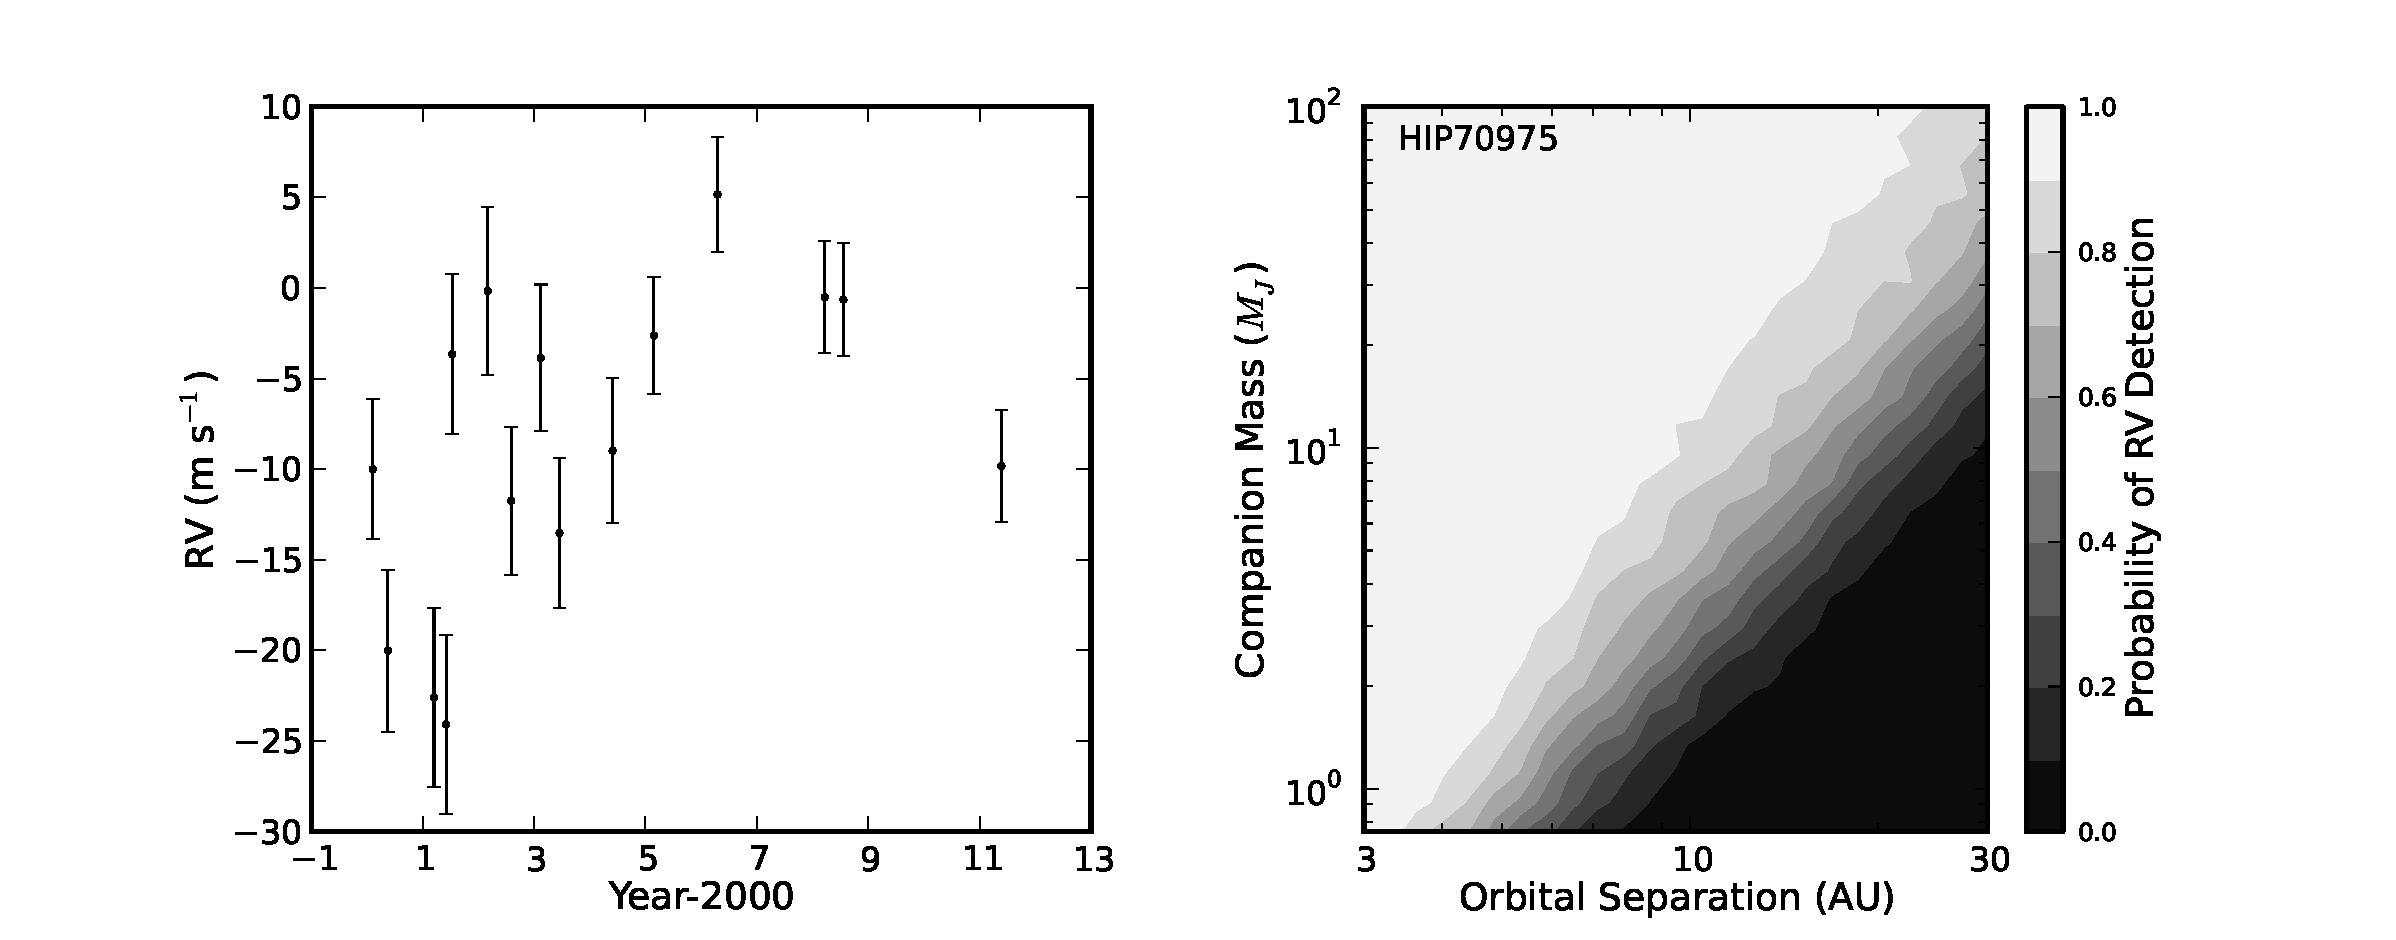
\includegraphics[width=\textwidth]{chapter3/f3.eps}}
\caption[RVs and detectability contours for a typical star in the survey]{(left) RVs for HIP\,70975, a typical star in our survey. This $0.32 M_\odot$ M-dwarf has a total of 15 radial velocity observations over a baseline of 15.5 years, with an average RV precision (including photon noise and jitter) of 4 m/s. (right) Detectability plot showing the likelihood of an RV detection for a companion orbiting HIP\,70975 as a function of companion mass and semimajor axis from its host star. \newline
  }
\label{Detectability}
\end{figure}


\begin{figure}[htbp]
        \centering      
\centerline{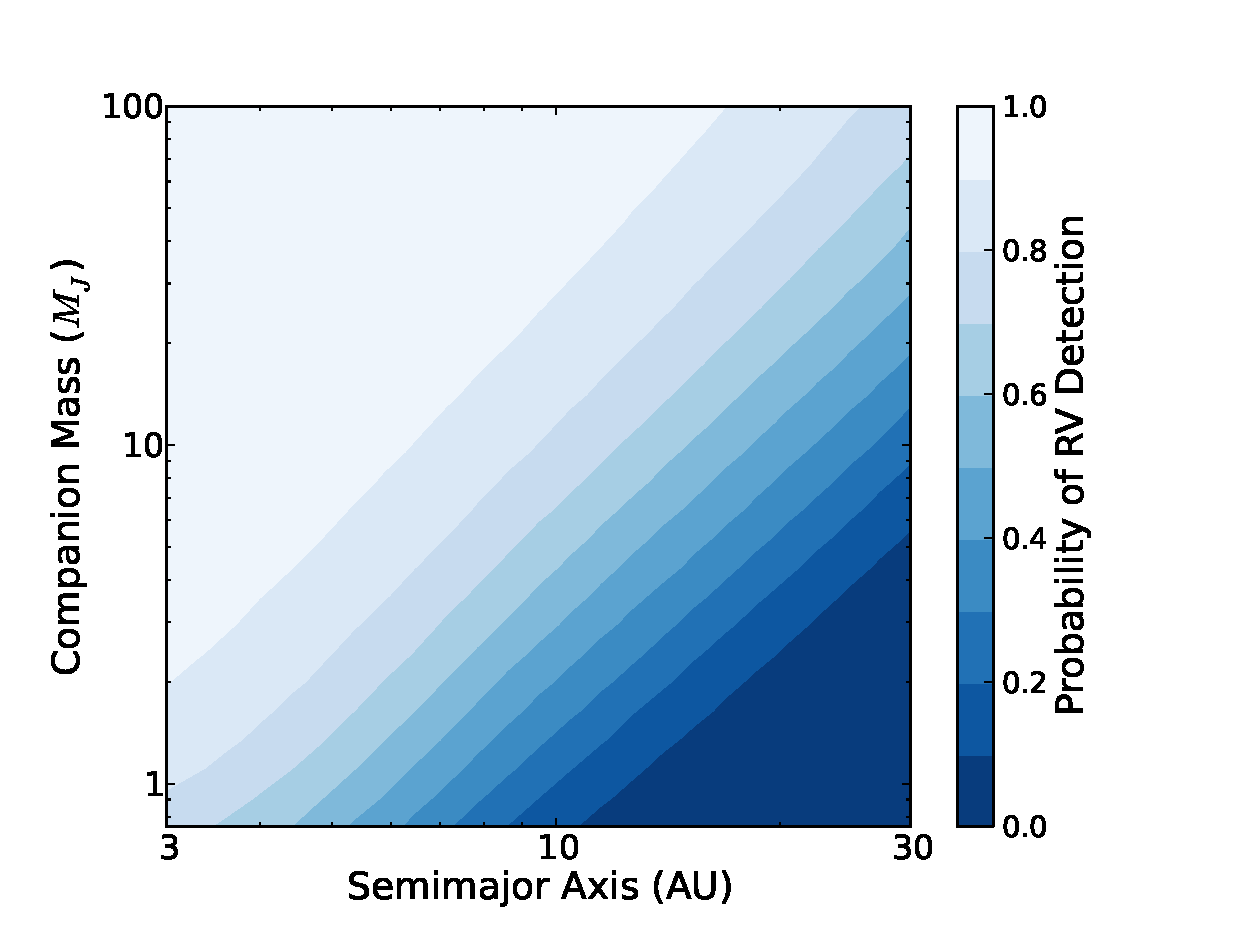
\includegraphics[width=0.75\textwidth]{chapter3/f4.eps}}
\caption[Ensemble likelihood detectability contours for an RV companion,
averaged over all stars in the sample]{The ensemble average likelihood over all 111 stars of an RV detection for a companion to a star in our sample as a function of companion mass and orbital semimajor axis. We can detect accelerations induced by planets as small as $1 M_J$ in short orbits, but a planet distribution function is required to determine the number of $1 M_J$ planets in wide orbits and calculate the overall giant planet occurrence rate.
  }
\label{DetectFull}
\end{figure}

Eight of the stars in our sample host known planets with closed orbits. All of the planets have $m \sin i < 2.5 M_J$ and are listed in Table \ref{knownpl}. To identify radial velocity accelerations caused by outer planets, we include the signal from these planets by comparing a model which contains the known planet and an acceleration to a model which contains only the known planet. Two known planets in our sample, Gl 876b and Gl 317b, are larger than $1 M_J$, so in addition to searching these systems for long-term RV accelerations, we also include these known planets in our giant planet occurrence calculations.
 

One additional planet, Gl\,649b, has a best-fitting mass $m \sin i = 0.90 \pm 0.05 M_J$; if the inclination is smaller than 64 degrees this planet has mass $ m > 1 M_J$. We follow the method of \citet{Ho11} to determine the probability of this event. That is, we define the probability that the true mass $m$ is greater than some value $X$ given an observed mass $m_O = m \sin i$ such that
\begin{equation}
P(m > X | m_O) = 1 - \frac{\int_{m_O}^X \frac{(m_O/m^2)}
{\sqrt{1-(m_O/m)^2}}P(m)dm}{\int_{m_O}^{m_\textrm{max}}
\frac{(m_O/m^2)}{\sqrt{1-(m_O/m)^2}}P(m)dm}
\end{equation}
Here, $P(m)$ is the true planet mass distribution function.
% We apply the distribution found by \citet{Cumming08}, as explained in \textsection{\ref{Methods}}. 
$m_\textrm{max}$ is the physical upper mass limit for a planet. Since the true distribution function is strongly biased towards small planets, the number selected here does not significantly affect our results. By simply assuming the star is aligned randomly along our line of sight so that the inclination distribution is flat in $\cos i$, the result of a flat planet mass distribution function, we expect a observed mass $m \sin i = 0.90 M_J$ to be produced by a Jupiter-mass or larger planet 56\% of the time; all reasonable assumptions of an underlying mass distribution affect this value by less than 10\%. We repeat this procedure for all confirmed planets in our sample with masses $m \sin i < 1 M_J$ to quantify the likelihood that other known planets are $m > 1 M_J$ planets with low inclinations. We find, in addition to Gl\,849b, HIP\,22627b ($m \sin i = 0.64 M_J$) has approximately a 25\% probability of having a mass $m > 1 M_J$. This probability is vanishingly small for all other known planets.

Of our sample of 111 stars, 2 have confirmed planets larger than $1 M_J$, 6 systems have confirmed RV planets with masses $m \sin i < 1 M_J$ only, two exhibit RV acceleration caused by known brown dwarfs, and four show unexplained long-term RV accelerations, such that $\Delta$BIC > 10 when we include an acceleration term in our fit to the RV data. In the case of Gl\,849b, the long-term acceleration exhibits significant curvature, so we are able to place constraints on this object's mass and orbital semimajor axis. In all other cases, the magnitude of the observed acceleration is different from zero by $3\sigma$. Additionally, the magnitude of the acceleration is such that over the observing baseline, the expected $\Delta\textrm{RV}$ induced by the putative outer planet is larger than the uncertanties of each individual data point. The distribution of these systems in the stellar mass-metallicity plane is shown in Figure \ref{massmetal}.

 
\begin{figure}[htbp]
\centerline{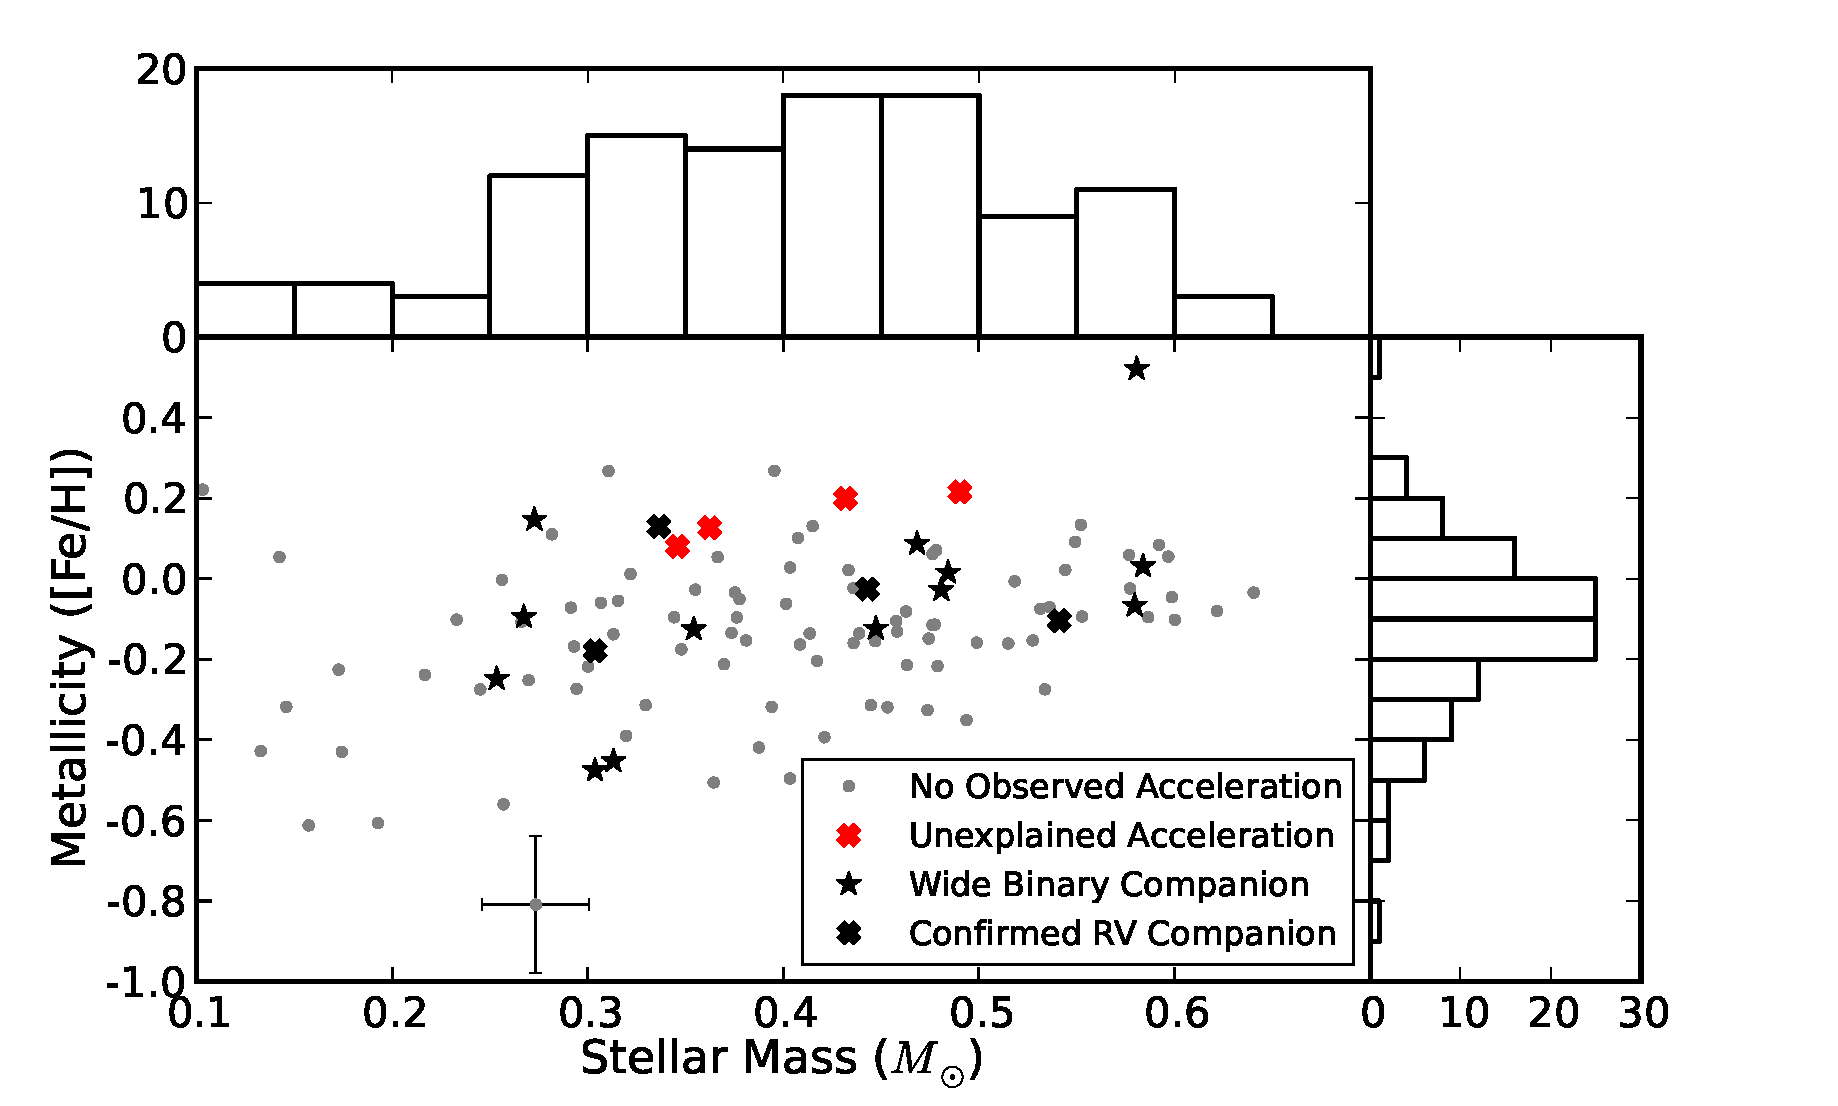
\includegraphics[width=0.95\textwidth,trim={0 0 0 0}, clip=true]{chapter3/f5.eps}}
\caption[Observed M-dwarf sample in the stellar mass-metallicity plane]{Observed M-dwarf sample in the stellar mass-metallicity plane. Systems with observed RV accelerations are shown in red while those without a detected acceleration are in black. Systems with a wide binary companion are labeled with stars, while diamonds represent systems with confirmed planets of any mass. The error bars displayed for HD\,33793 are representative of the uncertainties for all stars in our sample.
  }
\label{massmetal}
\end{figure}


For the four targets with an observable RV drift, we create a grid of logarithmically-spaced companion masses and semimajor axes over the range $0.75 < m/M_J < 100$ and $3 \textrm{AU} < a < 30 \textrm{AU}$. For a given grid point, we determine the best-fitting Keplerian orbit for a given eccentricity and inclination. We assume the inclination and eccentricity distributions are the same as assumed previously. The eccentricity distribution is well-characterized for solar-type stars, but may not hold for planets around lower-mass stars. We find the exact choice of eccentricity distribution does not significantly affect our results.

We determine the likelihood of the best-fitting orbit for each mass, period, eccentricity, and inclination. We then convert these likelihoods into relative probabilities, assuming our errors are uncorrelated so that $P \propto(-\exp(\chi^2/2)))$. We then marginalize over eccentricity and inclination and normalize our probabilities so that $\displaystyle\sum\limits_{M,a} P = 1$. In these cases, we assume the inclination is random on the sky, so that the inclination follows the distribution $f(i) = \sin i$. Assuming a different planet mass distribution function affects this result by less than 10\%. The result is a contour in the mass-semimajor axis plane for the likelihood that a given object could cause the observed stellar radial velocity variation \citep{Wright07}. An example is shown in Figure \ref{WrightRV}. Implicit in this analysis is the assumption the radial velocity variation is dominated by the motion of a single, massive companion rather than the constructive interference of the RV signal of two or more smaller objects. We discuss false positive probabilities in \textsection\ref{FP} and conclude the assumption that one signal dominates the observed RVs is reasonable.

\begin{figure}[htbp]
\centerline{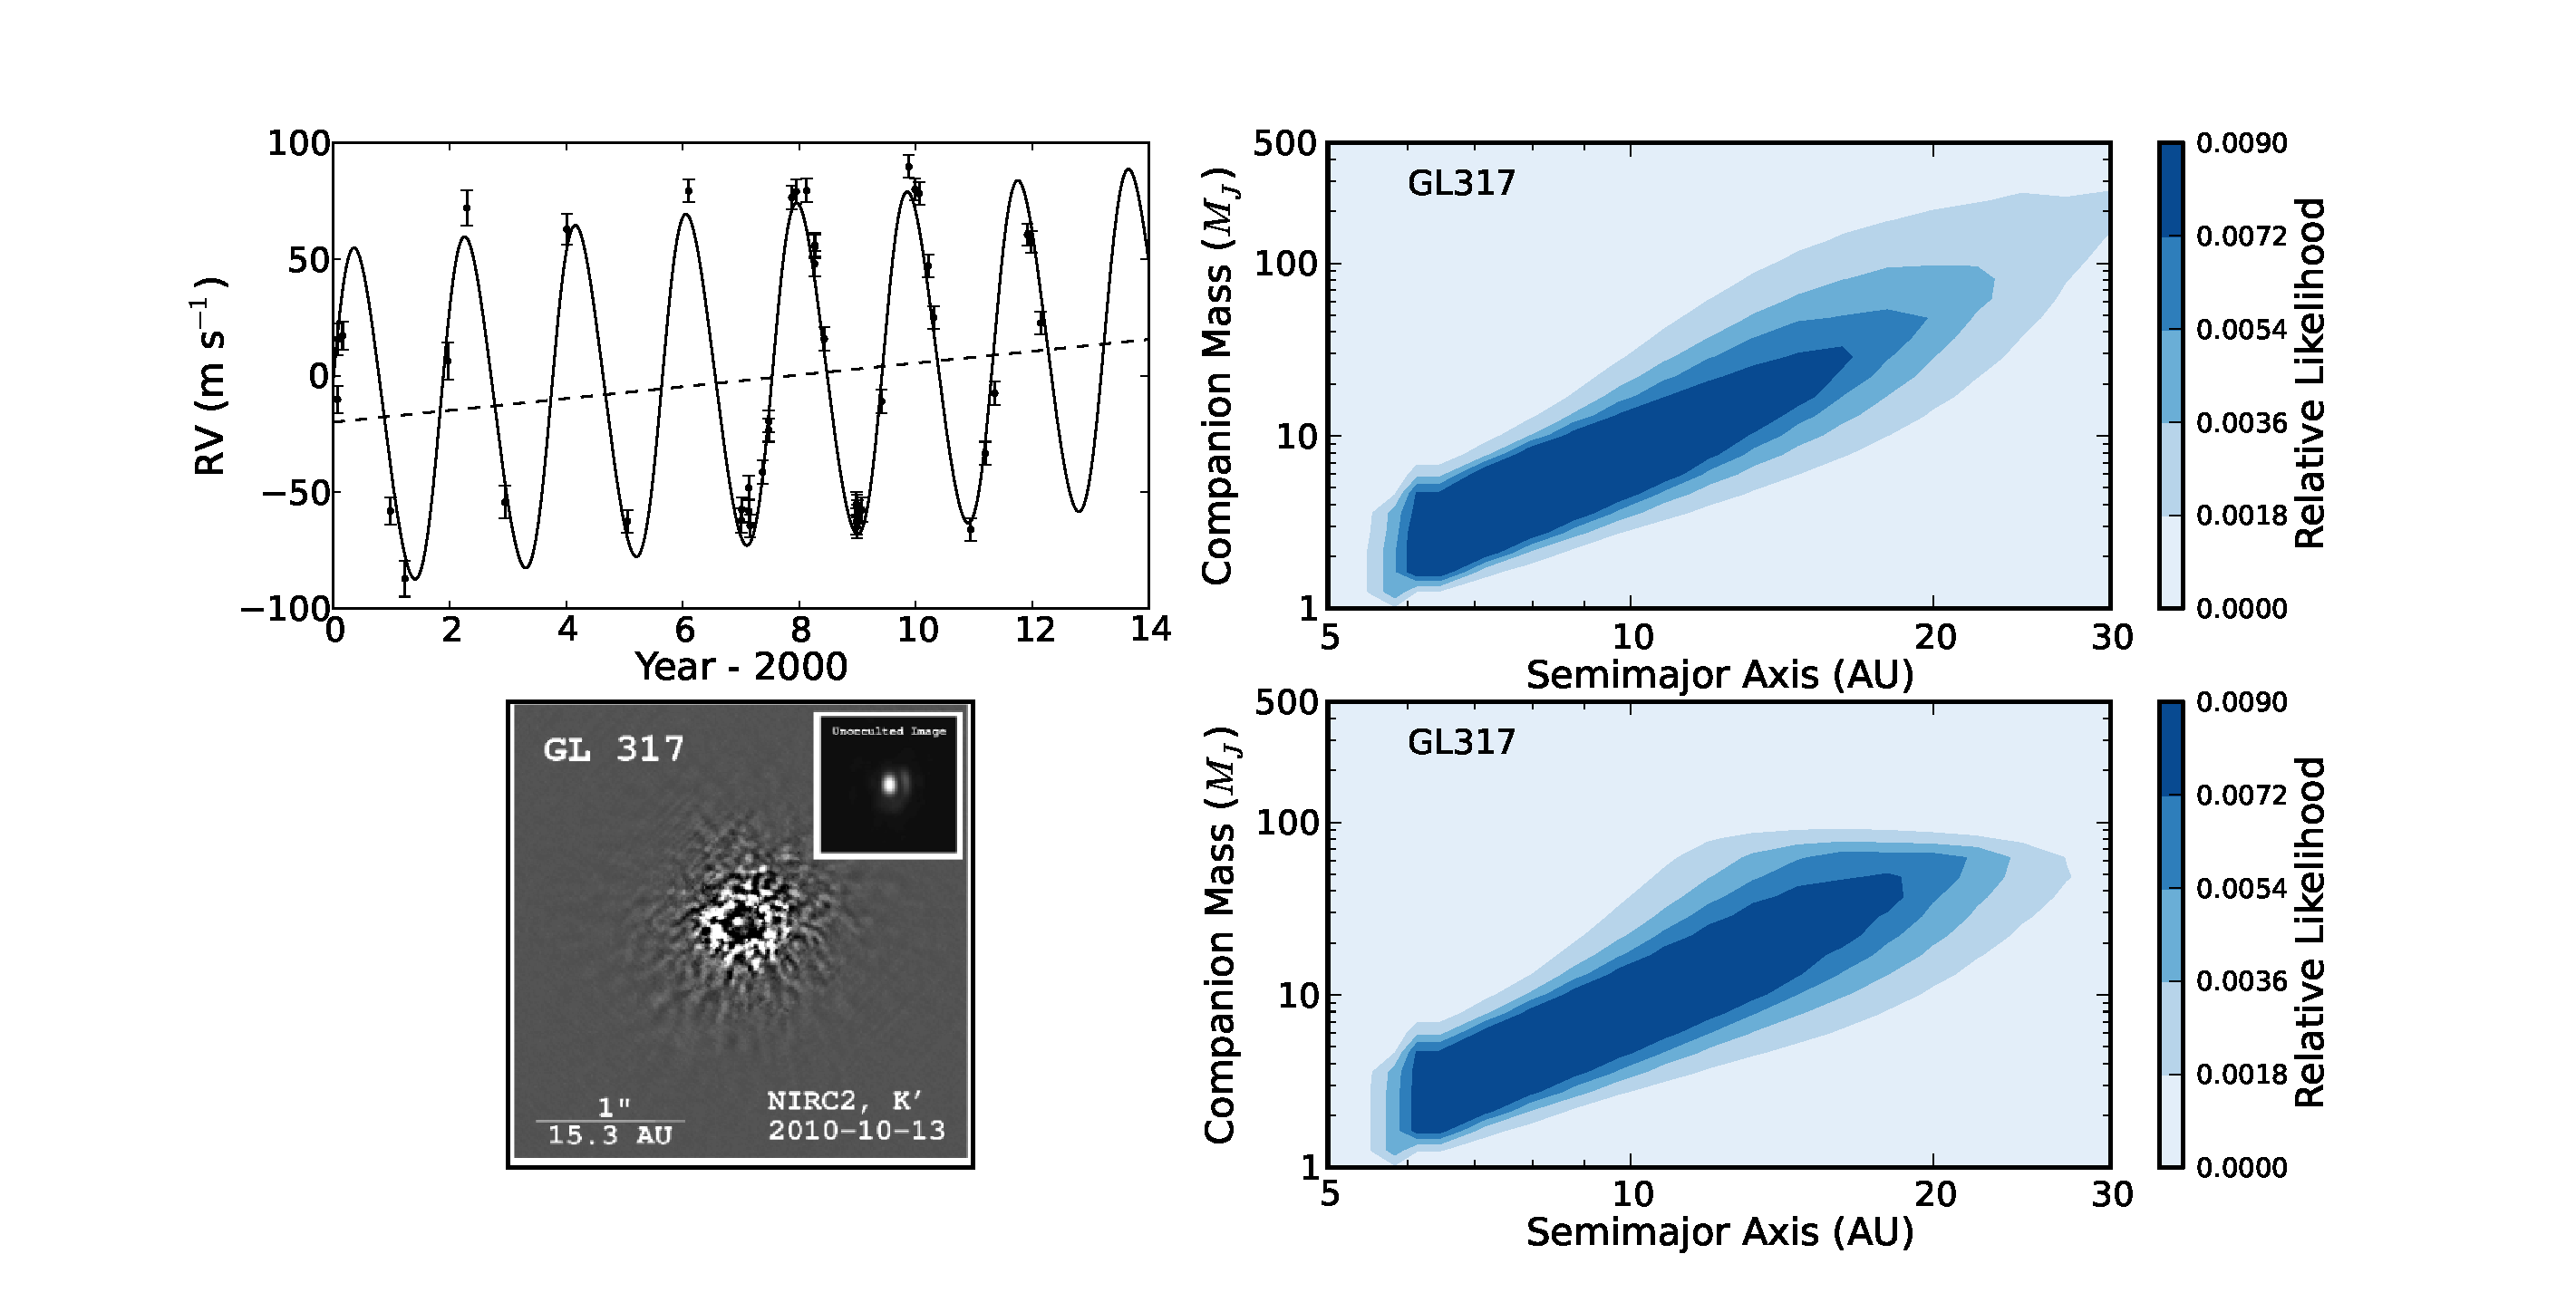
\includegraphics[width=1.0\textwidth, trim={0 0 0 0}, clip=true ]{chapter3/f6.eps}}
\caption[RVs for Gl\,317 and parameter space where a distant companion could reside before and after AO imaging]{(top left) RV observations for Gl\,317 over our 12.1 year baseline. The best-fitting RV acceleration is $-2.51 \pm 0.62$ m s$^{-1}$ yr$^{-1}$ (dashed line); the best-fitting model which includes both the planet and the acceleration is shown as a solid line. (top right) Probability contours marginalized over eccentricity and inclination, displaying the location of a giant companion orbiting Gl\,317 from RVs alone. The likelihood values are normalized such that the sum of the likelihood over our 26x25 grid of companion masses and separations sums to unity. (bottom left) AO image of Gl\,317, showing no companion is visible in the AO imagery, either in the unocculted image (inset) or when a coronagraph is inserted. This eliminates the possibility of a stellar-mass companion at a projected separation smaller than 48 AU. (bottom right) Probability contours displaying the location of a giant companion to Gl\,317 when the RV data is combined with AO data. We find the RV acceleration is likely induced by a substellar companion.
  }
\label{WrightRV}
\end{figure}


The magnitude of an acceleration depends on both the semimajor axis and mass of the companion. For a planet in a circular orbit, the magnitude of the change in radial velocity, $\dot{\gamma} = dv/dt$, is given by
\begin{equation}
\dot{\gamma} = (6.57 \mbox{ m} \: \mbox{s}^{-1} \mbox{yr}^{-1})\bigg(\frac{m_p}{M_J}\bigg)\bigg(\frac{a}{5 \mbox{AU}}\bigg)^{-2} \hat{v}_p \cdot \hat{r}_{los},
\label{TrendSize}
\end{equation}
with $M_J$ the mass of Jupiter and $a$ the orbital semimajor axis. $\hat{v}_p$ and $\hat{r}_{los}$ are unit vectors along the direction of the planet's velocity vector and the line of sight, respectively. When the companion has longitude of periapsis $\varpi = 90$ or $270$, the magnitude of this trend is maximized: $\hat{v}_p \cdot \hat{r}_{los} = \sin i$. To determine if our observed accelerations are caused by planets or more massive companions, we obtained AO imaging observations of each star.




\subsection{Adaptive Optics Observations}
\label{AO Description}
The detectability diagnostics developed in \textsection\ref{RVs} are based strictly on the information encoded in the RV data. Since we are looking at accelerations caused by objects in wide orbits around the primary star, we must break the degeneracy between companion mass and orbital semimajor axis for a given observed acceleration. AO imaging allows us to immediately detect the presence or nonexistence of nearly all stellar-mass companions and most brown dwarf companions to our primary stars, so we can readily separate stellar-induced accelerations from those caused by planets. 

All four targets with an observable RV acceleration were observed with NIRC2 (instrument PI: Keith Matthews) at the W.M. Keck Observatory using the AO system \citep{Wizinowich00} (Table \ref{T2}). In most cases, images were obtained in the $K^\prime$ filter ($\lambda_c = 2.12 \mu$m). We nominally execute a three-point dither pattern to facilitate removal of instrument and sky background noise. Images were processed by flat-fielding, correcting for hot pixels with interpolation, subtracting the sky background, and rotating the frames to standard north-east orientation. In three cases, we applied the angular differential imaging (ADI) point spread function subtraction technique, allowing the observed field to rotate around the target star during the observation, while instrumental artifacts remain fixed. In all cases, we use the large hexagonal pupil mask and the narrow camera. For all four systems exhibiting long-term RV accelerations, we did not image a massive companion. In the cases where our field of view is not large enough to eliminate the possibility of massive stars in very wide orbits ($ > 4''$), we supplement our AO data with publicly available 2MASS images. 
 

The luminosity ratio between our M-dwarfs and their companions depends on the mass of the companion and the age of the system. Stars observed by the CPS team are selected to avoid excessive chromospheric activity, and are thus likely older than 1 Gyr \citep{Wright05}. We assume all targets have fully contracted and assert an age of 5 Gyr for each system. For systems with nondetections, we estimate the flux (and thus the mass) a companion would need to have to be observed at a given projected separation in our observations. From that value, we can then determine the region of parameter space excluded by the observations (Figure \ref{CCplot}). In general, AO imaging eliminates nearly all stellar companions, while ADI can also probe the brown dwarf mass regime.

For each of our targets with unexplained accelerations, a contrast curve showing the mass to which we are sensitive to companions at the $5\sigma$ level as a function of projected separation is shown in Figure \ref{CCplot}. This choice provides similar results to the detection limits found by visual inspection, as tested by injecting artificial companions into AO images \citep{Metchev09}. We convert relative brightness to mass using the theoretical evolutionary tracks of \citet{Baraffe03} for substellar companions and \citet{Girardi02} for more massive companions. Interpolation between the two sets of models provides reasonable results in the intermediate domain near $125 M_J$. The resultant parameter space where a companion could reside to cause the observed stellar acceleration is shown in Figure \ref{WrightRV}. 



\begin{figure}[htbp]
\centerline{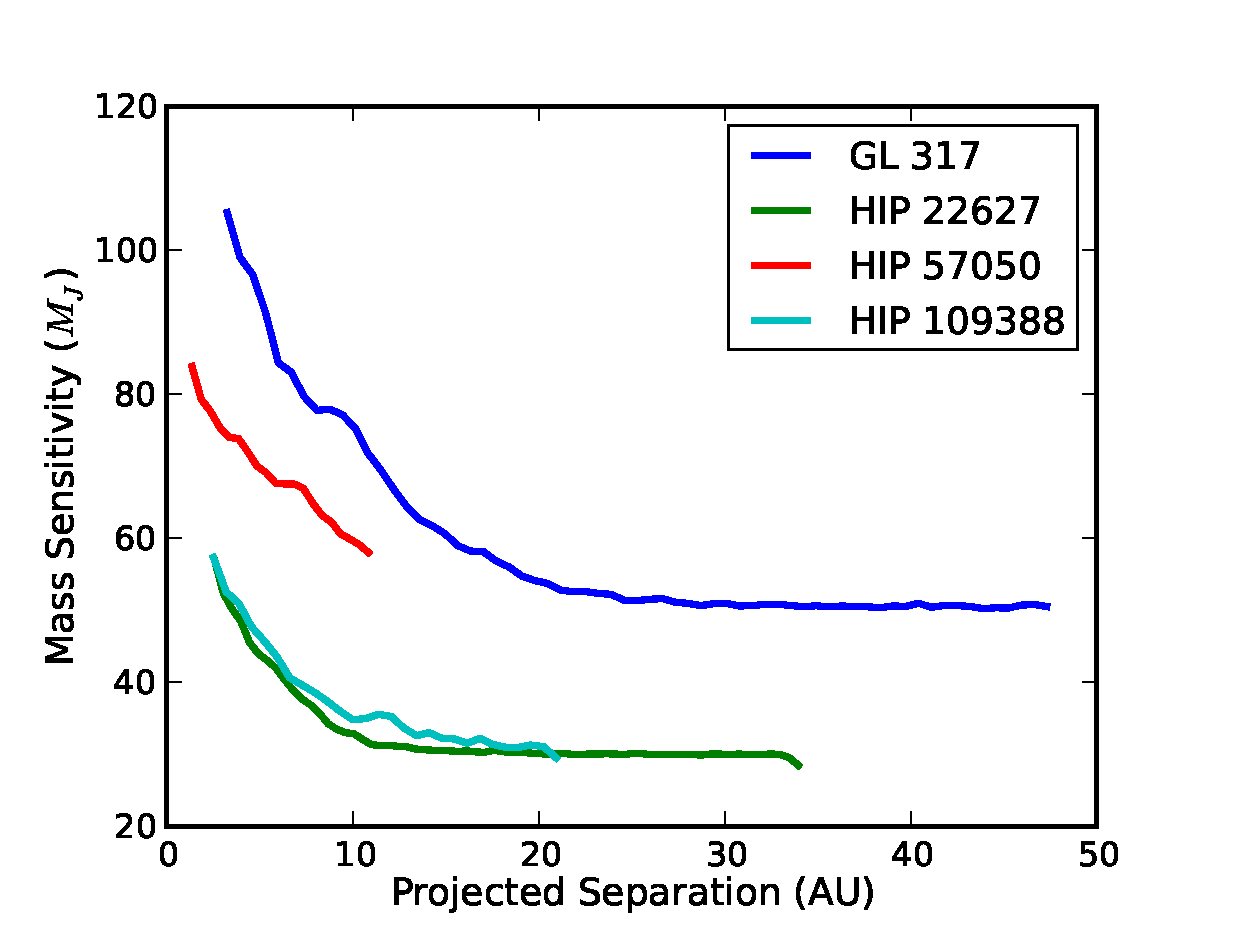
\includegraphics[width=0.75\textwidth]{chapter3/f7.eps}}
\caption[Mass sensitivity for a $5\sigma$ AO detection of a companion
as a function of projected angular separation]{Mass sensitivity for a $5\sigma$ detection of a companion object as a function of projected angular separation for each of our four stars with long-term RV drifts. The maximum projected separation eliminated corresponds to the field of view of the AO system and thus varies for each star as a function of the distance to each star. For all stars except HIP\,57050, we rule out stellar mass companions beyond 1 arcsecond through our adaptive optics imaging. When our field of view is small, we supplement our AO data with 2MASS seeing-limited images. Stellar companions at small projected separations would have RV accelerations larger than those observed in our sample. 
  }
\label{CCplot}
\end{figure}

The assumption of a 5 Gyr age for each star does not significantly affect our results. For all plausible system ages, stellar mass companions would be easily detectable by AO. Our sensitivity to stars is independent of assumed age, as luminosities of M-dwarfs are constant over the age of the universe. At no ages $> 1$ Gyr are we sensitive to any planetary mass companions. As shown in Figure \ref{AgeAO}, assuming a different age for each star would only change the efficiency of detecting brown dwarfs. Since the occurrence rate of brown dwarfs is only a few percent, much smaller than the occurrence rate of planets or low-mass stars \citep{Metchev09, Dieterich12}, errors induced by assuming an incorrect stellar age from missed brown dwarfs are small. ``False negatives'' such as these will be discussed in \textsection\ref{FN}.

\begin{figure}[htbp]
\centerline{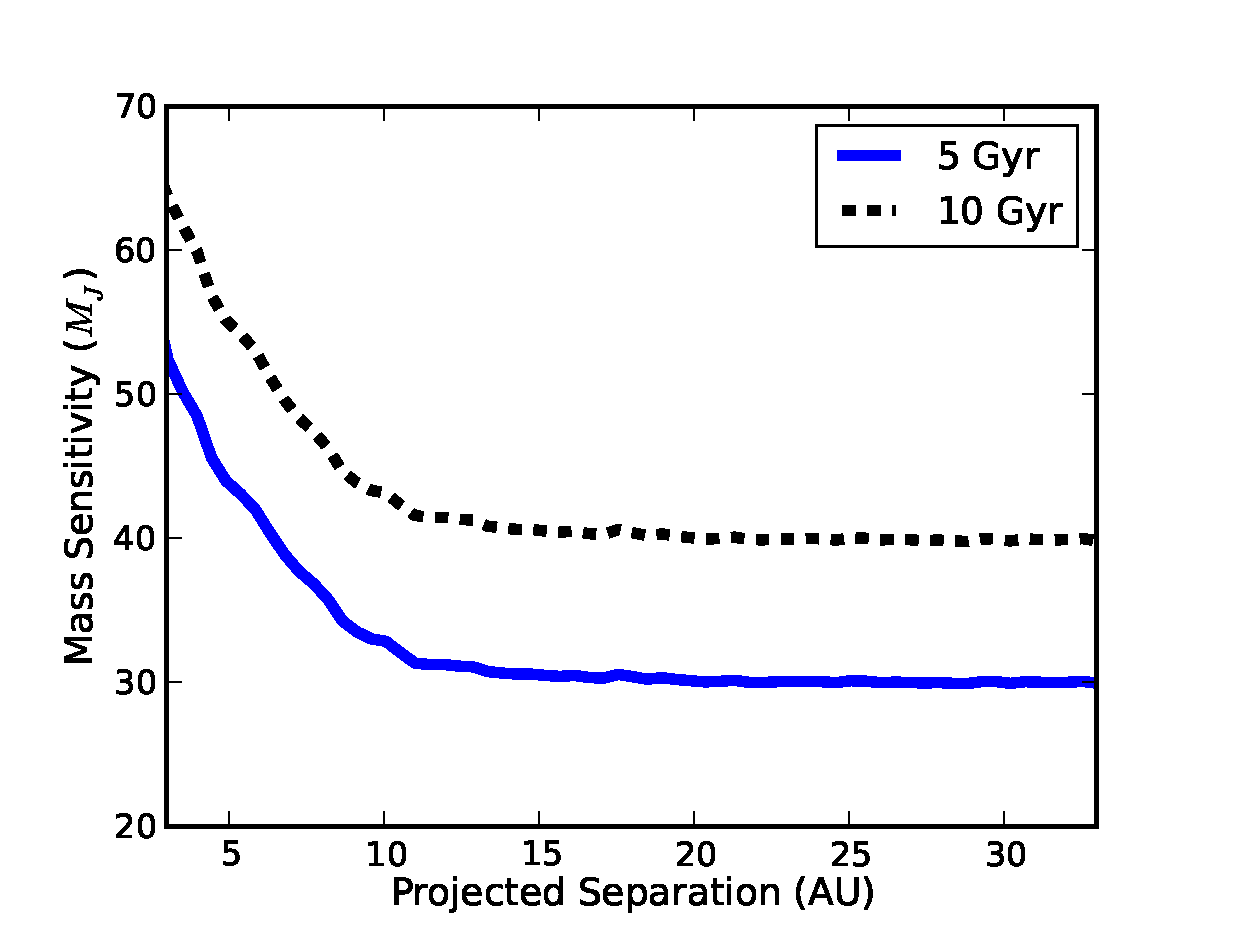
\includegraphics[width=0.75\textwidth]{chapter3/f8.eps}}
\caption[Mass exclusion plot for HIP\,22627 showing the insensitivity of our results to assumed stellar age]{Adaptive optics mass exclusion plot for the star HIP\,22627 showing the relative insensitivity of our results to the assumed age of M-star planet hosts. Adaptive optics observations rule out essentially all stellar mass companions. Sensitivity to substellar objects is a function of age, but brown dwarfs are scarce at close separations \citep{Marcy00}, and wide separations \citep{Metchev09}. Thus, our estimate of the planet frequency around M-stars is only weakly dependent on our assumed age of the host stars.  
  }
\label{AgeAO}
\end{figure}



\section{Measuring the Giant Planet Occurrence Rate}
\label{Stats}

We estimate the occurrence rate of giant planets orbiting M-dwarfs using statistical inference. The fraction of stars which host giant planets, given some number of observed accelerations $N\scriptsize{\mbox{trends}}$ and some number of nondetections $N\scriptsize{\mbox{ND}}$ from a sample of targets, is given such that
\begin{equation}f_{pl} = \frac{N\scriptsize{\mbox{trends}}\normalsize P(\mbox{planet}|\mbox{trend}) + N\scriptsize{\mbox{ND}}\normalsize P(\mbox{planet}|\mbox{ND})}{N\scriptsize{\mbox{targets}}}
\label{ResultEq}
\end{equation}
To calculate the posterior probability that a given star hosts a gas giant planet, we must estimate the \textit{a priori} likelihood that a planet exists given the presence of an RV acceleration (a true positive), the likelihood a planet would not be detected in an RV survey (a false negative) and the likelihood that an observed acceleration is caused by some effect other than the movement of a planet (a false positive). 

\subsection{False Negatives}
\label{FN}

There are multiple ways for a giant planet to be missed in our survey. For each planet in a wide orbit, we observe only a fraction of a revolution. A planet near its maximal sky-projected separation from its host star has acceleration primarily in the tangential, not radial, direction. In cases such as this the change in radial velocity over our observing baseline may not be noticeable. Thus we may expect to have a lower RV detection efficiency for planets near their maximal sky-projected separation. 

Similarly, we may expect to have a lower imaging detection efficiency for stars near their minimal sky-projected separation, when the RV acceleration is the largest. However, in these cases we would still expect to detect the binary companion. If the companion is located directly along the line of sight to the star, then it will also appear in the 0''.85 spectrograph slit used with HIRES. Therefore, we would expect such systems to appear as SB2s. We explore this fully, and show that we would detect all such systems, in \textsection\ref{PMBS}.

To determine the likelihood that such a planet would be missed by our search, we use our detectability matrices developed in \textsection\ref{RVs}. We assume the distribution of planets follows a double power-law, such that
\begin{equation}
\frac{d^2N}{d\log m d\log a} \propto m^{\alpha} a^{\beta},
\label{DPL}
\end{equation}
similar to that assumed by \citet{Cumming08} and \citet{Bowler10}, and comparable to the power-law distributions applied in the analyses of microlensing surveys. At a given companion mass and semimajor axis, we can then determine the relative likelihood that a planet exists at this position. We multiply this by the likelihood of detecting such a planet to determine the fraction of planets we would find orbiting each star and the fraction we would miss. These numbers are determined through our analysis of observations of simulated injected planets, as developed in \textsection \ref{TS}.

We can test our detectability calculation by analyzing the known wide-separation companions in our sample. Of our 111 stars, four are known to host directly imaged brown dwarf companions. Of these, two (HD\,71898B and HIP\,63510B) were detected as accelerations in our sample, while two (Gl\,569B and Gl\,229B) are at very large separations and were not detected. The detection or nondetection of each system is consistent with what would be expected from our analysis of injected planets.



We detect the two brown dwarfs with high expected RV detection efficiency, and do not detect the two with expected detection efficiencies near zero, both of which have $a > 40$ AU. We would like a larger sample to test this method, but the limited number of brown dwarfs suggests our ability to detect giant planets is consistent with expectations. This sample also suggests $f_{BD}$ is only a few percent, consistent with complementary studies \citep{Dieterich12}.


A giant planet could also be missed if it was in a system with multiple giant planets. We observe only the sum of all radial velocity signals from all planets orbiting a star. For example, if a star hosts two giant long-period planets with one on each side of the star, the two signals would destructively interfere. Even if the acceleration was still detectable, this interference would cause us to measure an incorrect magnitude of the acceleration, so our probability contours would be incorrect. Giant planet multiplicity around M-dwarfs is not well understood, but since giant planet occurrence is believed to be small \citep{Bonfils13} the multiplicity rate of giant planets around M-dwarfs is likely also small. Presently, there are no known systems with two planets larger than Jupiter orbiting one M-dwarf. Even in cases with two large planets, one planet will dominate the RV signal. For example, OGLE-2006-BLG-109L contains a $0.73 \pm 0.06 M_J$ planet at $2.3 \pm 0.5$ AU and a $0.27 \pm 0.02 M_J$ planet (slightly less massive than Saturn) at $4.5^{+2.1}_{-1.0}$ AU \citep{Gaudi08, Bennett10}. In this case the Doppler amplitude of the inner planet would be a factor of 3.3 larger than the Doppler amplitude of the outer planet. Similarly, an external observer of the solar system would observe an RV signal from Jupiter 4.5 times larger than that of Saturn. Thus we neglect this possible source of error.


We then claim that the likelihood of the existence of a giant planet given the nondetection of an RV acceleration is 
\begin{equation}
P(\mbox{planet}|\mbox{ND}) = f_{pl}(1-\eta_{pl,\star})
\label{FNP} 
\end{equation}
where $\eta_{pl, \star}$ is the probability of detecting a giant planet around a given star as a function of planet mass and orbital semimajor axis, estimated by simulating observations of injected planets. The true probability of missing a planet depends on the true giant planet occurrence rate and the planet distribution function. We can determine this value directly if the underlying planet distribution function (Equation \ref{DPL}) is assumed. By counting the observed trends and analyzing our RV detection efficiencies for each star as a function of mass and separation, we can determine the number of missed planets. We find our final result is not a strong function of mass index $\alpha$ or semimajor axis index $\beta$ (see \textsection\ref{PL}).

\subsection{False Positives}
\label{FP}
\subsubsection{Multiple Planets}
In some cases, observed accelerations may not be induced by the orbit of a giant planet. If two smaller planets are orbiting one star, when they are both on the same side of the star their RV signals would constructively interfere, giving the appearance of a giant planet where none exists. Again, multiplicity rates of large planets are unknown for these small stars but are likely small; we again neglect this effect as a possible source of error. This is a reasonable assumption even if the multiplicity rate of gas giant planets around M-dwarfs was much larger than currently expected. Both the orientation of the system and the relative positioning of the planets during our observations is random. Therefore, it is equally likely that multiple planets would be in the ``constructive'' or ``destructive'' phase of their orbits. Thus, similar numbers of false additional planets would be added to our sample as missed true planets. 

\subsubsection{Secular Acceleration}
A false positive can also be caused by secular acceleration. When a high proper motion star moves quickly relative to the Sun, its peculiar velocity vector changes direction in time, causing the star's systemic radial velocity to increase. For a star with proper motion $\mu$ at a distance $d$ the magnitude of this effect is, to first order,
\begin{equation}
\dot\gamma = 23.0 \textrm{ cm s}^{-1} \textrm{ yr}^{-1} \bigg(\frac{d}{10\textrm{ pc}}\bigg)\bigg(\frac{\mu}{1 \textrm{ arcsec yr}^{-1}}\bigg)^2.
\end{equation}
The secular acceleration $\dot\gamma$ is always positive, so that the star's radial velocity only increases because of this effect. For several nearby stars secular acceleration is large enough to create an apparent acceleration or cause an astrophysical RV acceleration to be incorrectly measured. For example, Barnard's star has a secular acceleration of $4.515 \pm 0.002$ m s$^{-1}$ yr$^{-1}$ \citep{Choi13}, larger than all of our observed accelerations. Fortunately, the magnitude of the secular acceleration can be precisely quantified if the star's distance and proper motion are known. All of our stars have measured proper motions and parallaxes, so we can determine the expected secular contribution. This acceleration is subtracted from the observed radial velocity automatically by the CPS RV pipeline \citep{Howard10}, so this potential source of error is automatically accounted for in our data. Moreover, none of our observed accelerations are consistent with what would be expected from secular acceleration alone. 

\subsubsection{Magnetic Activity}
\label{MA}
Magnetic activity on a star can cause a false positive: rotating active regions can affect the shape of the observed spectral lines and thus the apparent RV \citep{Gray88}. A magnetic cycle can occur over years and hide or mimic a radial velocity signal. We denote the fraction of stars with a magnetically-induced acceleration as $f_A$. \citet{GomesdaSilva12} claim six stars from their sample of 27 M-dwarfs with variability ($22\% \pm 9\%$) have RVs induced by magnetic activity. We are interested in the converse (how many trends are induced by variability?) but their result suggests $f_A$ may be significant. To determine $f_A$, we review all 165 M-dwarfs observed by the CPS team, both as part of this survey and as part of the M2K survey \citep{Apps10, Fischer12}. Between these two programs, there are a total of 34 systems with RV trends. We analyze the $S_{HK}$ values for these stars and find the RV correlates with $S_{HK}$ with a correlation coefficient $|r| > 0.5$ in 7 cases, suggesting $20.6\% \pm 7.8\%$ of long-term RV trends may be magnetically induced. We adopt this value as $f_A$. Even if the true value for $f_A$ is a factor of two larger, it would decrease our planet occurrence rate from $f_{pl} = 6.5\%$ to only $f_{pl} = 4.9\%$, still within our uncertainties.

\subsubsection{Brown Dwarfs}
\label{BD}
Our adaptive optics search is sensitive to all stellar-mass companions, but only to the most massive brown dwarfs. We can detect brown dwarfs larger than approximately $50 M_J$, although this number varies from target to target. For each target, we can determine the fraction of brown dwarfs we would expect to detect by our adaptive optics imaging, given the assumption that a trend was caused by a brown dwarf. We call this efficiency $\eta_{BD}$. Here, we assume a form for the brown dwarf mass function where $dn/d\log(m) \propto m^{0.4 \pm 0.2}$ \citep{Pena-Ramirez12}. Thus we can estimate the likelihood of detecting a brown dwarf around a star in our sample, given that a brown dwarf exists. To estimate the probability a brown dwarf exists, we use the result of \citet{Dieterich12}, who, through an HST/NICMOS snapshot program, estimate that $f_{BD} = 2.3^{+5.0}_{-0.7}\%$ (at $1\sigma$) of M-dwarfs have an L or T companion between 10 and 70 AU. This is consistent with the result of \citet{Metchev09}, who estimate a brown dwarf companion frequency of $f_{BD} = 3.2^{+3.1}_{-2.7}\%$ (at $2\sigma$) around solar-type (FGK) stars.

\subsubsection{White Dwarfs}
\label{WD}
Compact stellar remnants are often faint and such binary companions can evade direct detection, especially when the compact object is cool ($T < 4000 K$) so that the infrared light is dominated by the primary star \citep{Crepp13b}. Since our targets are all M-dwarfs, it is not unreasonable to expect that some may have formed as lower mass companions in binary systems with the higher mass object having evolved off the main sequence to become a white dwarf.  \citet{Napiwotzki09} combine observations of local white dwarfs with galactic structure models and find that in the thin disk there is a white dwarf number density of $n_{WD} = 2.9 \times 10^{-3}$ pc$^{-3}$. From an analysis of PanSTAARS data, \citet{Wheeler12} estimate 20\% of all white dwarfs have an M-dwarf companion ($f_{M|WD}$), somewhat larger than the 12\% found by \citet{Napiwotzki09}. Considering the measurement by \citet{Chang11} of $n_\star = 0.030 \pm 0.002$ stars per cubic parsec, and that approximately 70\% of all stars are M-dwarfs \citep[$f_{M|\star}$,][]{Henry06}, we can determine the fraction of M-dwarfs in the thin disk with a white dwarf companion, a number we define as $f_{WD}$. If we take $f_{M|WD} = 0.16 \pm 0.04$, we find that 
\begin{equation}
f_{WD} = \frac{n_{WD}f_{M|WD}}{n_\star f_{M|\star}} = 2.2\% \pm 0.5\%,
\end{equation}
where the error is dominated by the uncertainty in $f_{M|WD}$.

By combining the false positive events from \textsection\ref{MA}, \textsection\ref{BD}, and \textsection\ref{WD}, we conclude that given the existence of a trend in our data, the likelihood it is caused by a giant planet is 
\begin{equation}
P(\mbox{planet}|\mbox{trend}) = (1-f_A)[1-f_{BD}(1-\eta_{BD, \star})](1-f_{WD})
\label{FPP}
\end{equation}

\subsection{Determining $f_{pl}$}
\label{Methods}

We determine the giant planet occurrence rate, $f_{pl}$ by combining our estimate of the number of false positives and false negatives with the number of observed accelerations. Specifically, the occurrence of giant planets is given by Eq. \ref{ResultEq} if the number of observed accelerations is known, along with the probability of a false negative or false positive in our sample. These probabilities are defined by Equations \ref{FNP} and \ref{FPP}, respectively. 

For each star in our sample, we use our map of giant companion detectability (e.g. Figure \ref{WrightRV}) to estimate our efficiencies, $\eta_{BD}$ and $\eta_{pl}$. We measure the total planet fraction, $f_{pl}$ and its uncertainty through a Monte Carlo experiment. For each trial, we establish an expected number of observed accelerations, drawing from a binomial distribution with $n=111$ and $p = 4/111$, representing the most likely underlying distribution behind our observed sample. In practice, we draw from our star list 111 times, with replacement, to determine a stellar sample. We then draw randomly from our previously defined distributions to estimate $f_A$, $f_{BD}$ and $f_{WD}$. These values are sufficient to calculate the probability an observed acceleration is caused by a false positive astrophysical event. In cases where known planets with masses $m > 1 M_J$ exist in our sample, we include their presence in our calculation of $f_{pl}$. 

The derivative of the RV acceleration (the ``jerk'') for Gl\,849 is nonzero, so we can use the RV information to fit a two-planet model to this system, instead of a planet plus a linear acceleration. We find the inner planet to have a mass $m\sin i = 0.90 \pm 0.05 M_J$ with a period of $5.24 \pm 0.07$ years, and the outer planet to have a mass $m \sin i = 0.70 \pm 0.31 M_J$ with a period of $19.3^{+17.1}_{-5.9}$ years. More data is needed to determine the exact parameters of the orbit of Gl\,849c, but from the existing RV information we can determine the probability each planet has a mass $m > 1 M_J$. The exact value depends on the planet mass distribution function; assuming each orientation has equal probability (so that $\alpha=-1$) we find probabilities of 0.577 and 0.419, respectively. Following the method of \citet{Ho11}, we find changing the distribution function changes these values by less than 10\%. 

% Make sure there's nothing here for @OverheardOnAph to pick up

Since we know the region of mass-separation parameter space to which we are sensitive to planets for each star, we can self consistently estimate the planet frequency in this parameter space. We then assume the result from \citet{Cumming08}, who find the power-law indices (Eq. \ref{DPL}) of $\alpha = -0.31 \pm 0.20$ and $\beta = 0.39 \pm 0.15$. We randomly select values for $\alpha$ and $\beta$ from these distributions and use our detection efficiencies to determine the number of false negative missed planets in our sample. Through Equation \ref{ResultEq}, we then have enough information to estimate the planet fraction as a function of each parameter. By repeating this process many times, varying each of our assumed parameters, we can measure the overall planet fraction and its uncertainty.


\section{Results and Discussion}
\label{Results}
\subsection{The Frequency of Giant Planets}
\label{R1}

Given an observed trend, we can estimate the likelihood the signal is caused by a massive planet. By analyzing our 111 targets as described in \textsection\ref{Methods}, we recover a distribution in giant planet occurrence as shown in Figure \ref{HistoResult}. We find from this analysis that $6.5\% \pm 3.0\%$ of all M-dwarfs host a giant planet with a semimajor axis smaller than 20 AU. This number is lower than previous studies of higher-mass stars. \citet{Bowler10} find $24^{+8}_{-7}\%$ of ``retired'' A stars host Jupiter-mass planets within 3 AU, while \citet{Cumming08} find that $f_{pl} = 10\% \pm 1\%$ of FGK stars host Jupiter-mass planets within 20 AU. 

If we consider multiplicity in situations where we have a giant planet and an RV acceleration (or in the case of Gl\,849, two giant planets), then we measure a giant planet occurrence rate of $0.083 \pm 0.019$ giant planets per star. To estimate this, we repeat the calcuations of the previous section, but count known giant planets separate from observed accelerations in the cases when we observe both a planet and a ``trend.'' This number does implicitly assume that observed accelerations are caused by the motion of one giant planet, not a combination of multiple planets in motion. The multiplicity rate of giant planets around M-dwarfs appears to be lower than the multiplicity rate of small planets, such as those detected by \textit{Kepler} \citep{Youdin11}.

Our result is consistent with the result of microlensing surveys of M-dwarfs, which suggest a total occurrence rate of $0.09^{+0.03}_{-0.05}$ giant planets per star in the range $1 M_J < m < 10 M_J$ and $0.5$ AU $< a < $20 AU \citet{Cassan12}. However, the power-law distribution determined by the microlensing studies is considerably different than the \citet{Cumming08} distribution assumed here. We discuss this further and constrain $\alpha$ and $\beta$ in \textsection \ref{muL}.

\begin{figure}[htbp]
\centerline{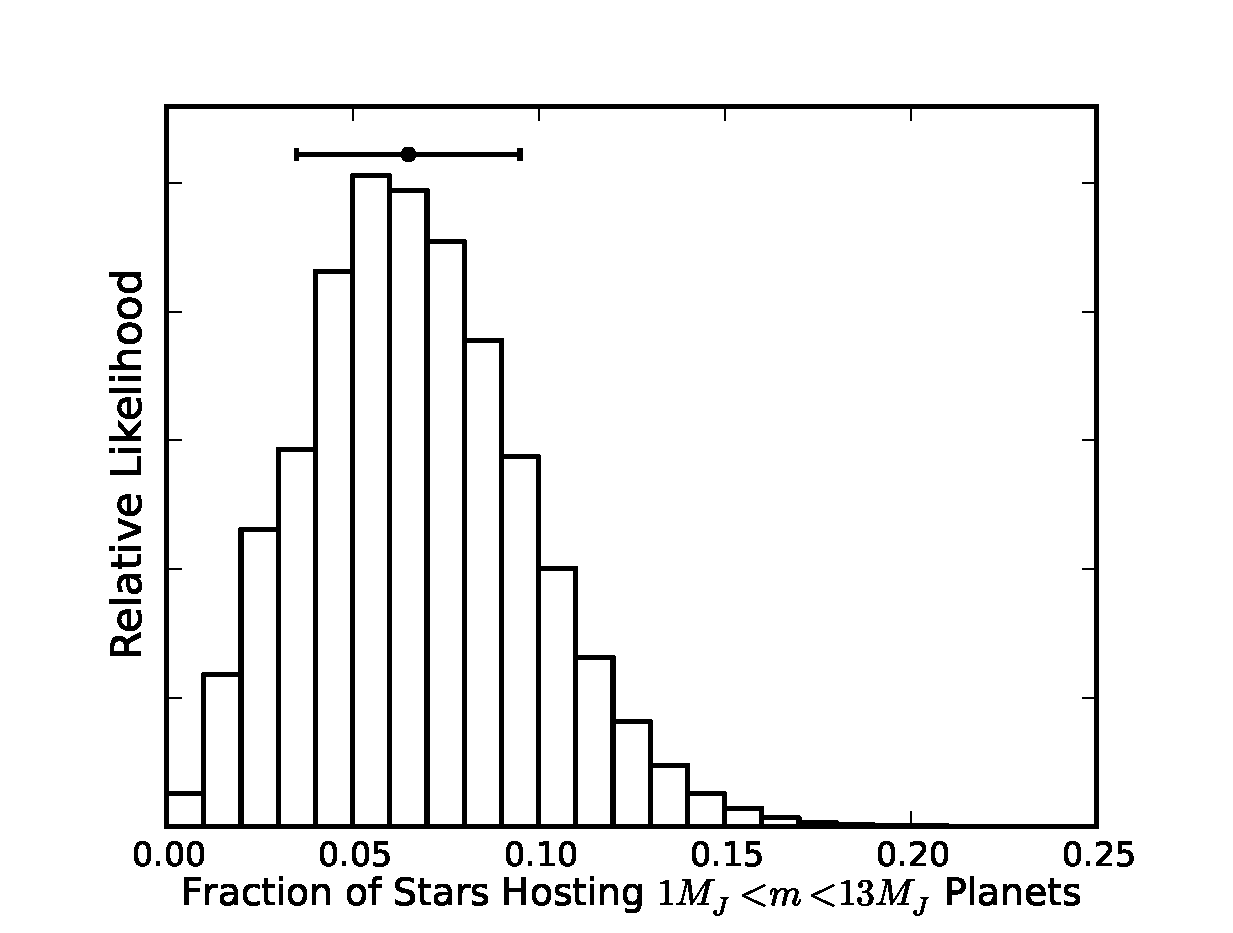
\includegraphics[width=0.75\textwidth]{chapter3/f9.eps}}
\caption[Posterior distribution of the occurrence rate of giant planets
orbiting M dwarfs]{Giant planet occurrence for our sample of 111 nearby M-dwarfs. We find $6.5\% \pm 3.0\%$ of M-dwarfs host a planet with mass $1 M_J < m < 13 M_J$ and $0 < a < 20$ AU.}
\label{HistoResult}
\end{figure}

This is the first study using observed RV accelerations to estimate the giant planet occurrence rate. However, previous RV studies have discussed the presence or nondetection of RV accelerations in their analysis. For example, \citet{Endl03} mentioned all RV accelerations in their sample are likely the cause of stellar binaries. Our observations are generally more precise than theirs, as we detect some planets that they miss (such as Gl 436 and Gl 849).

\citet{Bonfils13} detect 15 long-term accelerations in their sample of 102 southern M-dwarfs. Some of these can be attributed to long period binary companions (such as Gl\,250B and Gl\,618A). Of the stars where we detect an RV acceleration, only one (Gl\,849) is in the HARPS sample; these authors also detect an acceleration. \citet{Bonfils13} also detect an acceleration around Gl\,699 (Barnard's star) that we do not detect. Such an acceleration has also not been found by other studies: \citet{Choi13} claim the RV of Barnard's star is increasing at $4.515 \pm 0.002$ m s$^{-1}$ yr$^{-1}$, consistent with the expected secular acceleration but inconsistent with the $-3.043 \pm 0.646$ m s$^{-1}$ yr$^{-1}$ acceleration observed by \citet{Bonfils13}. With more observations over a longer time baseline, this discrepancy will be resolved.



\subsection{Potential Missed Binary Stars}
\label{PMBS}
We only collect AO images for systems with long term RV accelerations. For these accelerations to be observable, the orbiting companion must have a component of its movement along our line of sight so that the radial velocity changes during an orbit. A giant planet would be missed if it was in a near face-on orbit, such that the star's reflex motion was primarily in the plane of the sky. Such systems are accounted for in our detectability calculations (Figure \ref{Detectability}), as we have determined the probability of detecting a planet's RV acceleration as a function of its mass and separation, marginalized over all other orbital parameters. These calculations do not, however, account for the possible presence of close stellar binary companions in face-on orbits. Although less common than edge-on systems, any missed binary systems that we have not rejected from our sample would cause our planet occurrence rate to be artificially low (assuming these systems could not form dynamically stable planets). Close binaries would be observable as double-lined spectroscopic systems (SB2s) in the CPS data, while wider binary pairs would be easily imaged by AO systems.

The RV sample was originally selected to reject systems with known binary companions within 2 arcseconds. We would expect companions with a flux ratio larger than 0.01 ($\Delta V = 5$) to be detected as binaries \citep{Robinson07}. For our brightest targets, this would correspond to M6 dwarfs and brighter. As the cutoff for hydrogen burning is the M6 spectral class \citep{Luhman12}, we would expect all close stellar-mass binaries to be removed from our HIRES observations. 

To determine how many missed binaries are in our sample, we simulate a population of binary companions to M-dwarfs. We create binary companions such that their semimajor axes are assigned following the observed distribution found by \citet{Fischer92}. We randomly assign the other orbital parameters and determine there is a $41.8\% \pm 0.3\%$ chance a binary companion in our sample around a random star would have a projected separation smaller than two arcseconds. Thus, considering \citet{Fischer92} find $42\% \pm 9\%$ of local M-dwarfs are in binary or multiple systems, we would expect to have a total of $24 \pm 6$ binary systems in our sample, which originally contained 137 stars before the removal of known binaries. As we actually observe 22 binary systems (containing 26 stars), this result is consistent with our expectation.

We then determine the radial velocity each simulated binary star would induce on our host companion. For each binary that induces a measurable acceleration on the host star, we simulate imaging observations to determine the probability this binary companion would be detected in either our AO survey or, for very wide separation binaries, a seeing-limited ground based survey such as 2MASS. By applying our joint AO/seeing-limited contrast curves, we find that if a binary star system in our survey induces an RV acceleration, we would have a $96.0\% \pm 0.4\%$ chance of imaging this binary companion. Therefore the probability that one or more of our observed accelerations is caused by a ``missed'' binary companion is negligible and this possibility does not significantly affect our results.




\subsection{Dependence on Stellar Mass}
\label{MassDep}
Previous RV studies have found a correlation between stellar mass and giant planet occurrence at $a < 2.5$ AU, with more massive stars more likely to host giant planets \citep{Johnson10a}. To test this relation inside the M-dwarf spectral class, we analyzed the high mass stars separately from the low mass stars in our sample. From our best fit masses, half of our sample is more massive than $M = 0.41 M_\odot$. We thus use this value as a dividing line to separate our sample into two groups. Our masses have typical uncertainties of $10\%$, so for each star, given its mass and uncertainty, we determine the probability it is larger or smaller than $0.41 M_\odot$ assuming normally distributed errors. We then use that value as a weighting factor to assign a probability for each individual star to reside in our high mass or low mass bin, and then repeat our analysis for each individual subsample.

We find an occurrence rate for the high mass subsample of $4.8 \pm 3.3\%$ and for the low mass subsample of $7.9 \pm 4.2\%$ (Figure \ref{Mass}). \citet{Johnson10a} find planet occurrence is correlated with stellar mass such that $f_{pl} \propto 10^{(1.2\pm 0.2)\textrm{[Fe/H]}}M_\star^{(1.0\pm 0.3)}$. The average star in our high-mass sample has a mass of 0.5 $M_\odot$ while the average star in our low-mass sample has a mass of 0.3 $M_\odot$, so we would expect the high-mass subsample to have an occurrence rate larger than the low-mass sample by a factor of 1.67. We find the true occurrence rate to change by a factor of $0.61 \pm 0.87$ in moving from the lower-mass to higher-mass bin. This is inconsistent with the expected result from \citet{Johnson10a}, but the difference between the two bins is not significantly different from zero. A larger sample is required to determine if the small difference between these two populations of M-dwarfs is real or the result of a statistical anomaly. However, our result is lower than the \citet{Cumming08} result for FGK stars, that $f_{pl} = 10\% \pm 1\%$ of FGK stars host Jupiter-mass planets within 20 AU. This difference is consistent with the \citet{Johnson10a} correlation between stellar mass and planet occurrence. 


\begin{figure}[htbp]
\centerline{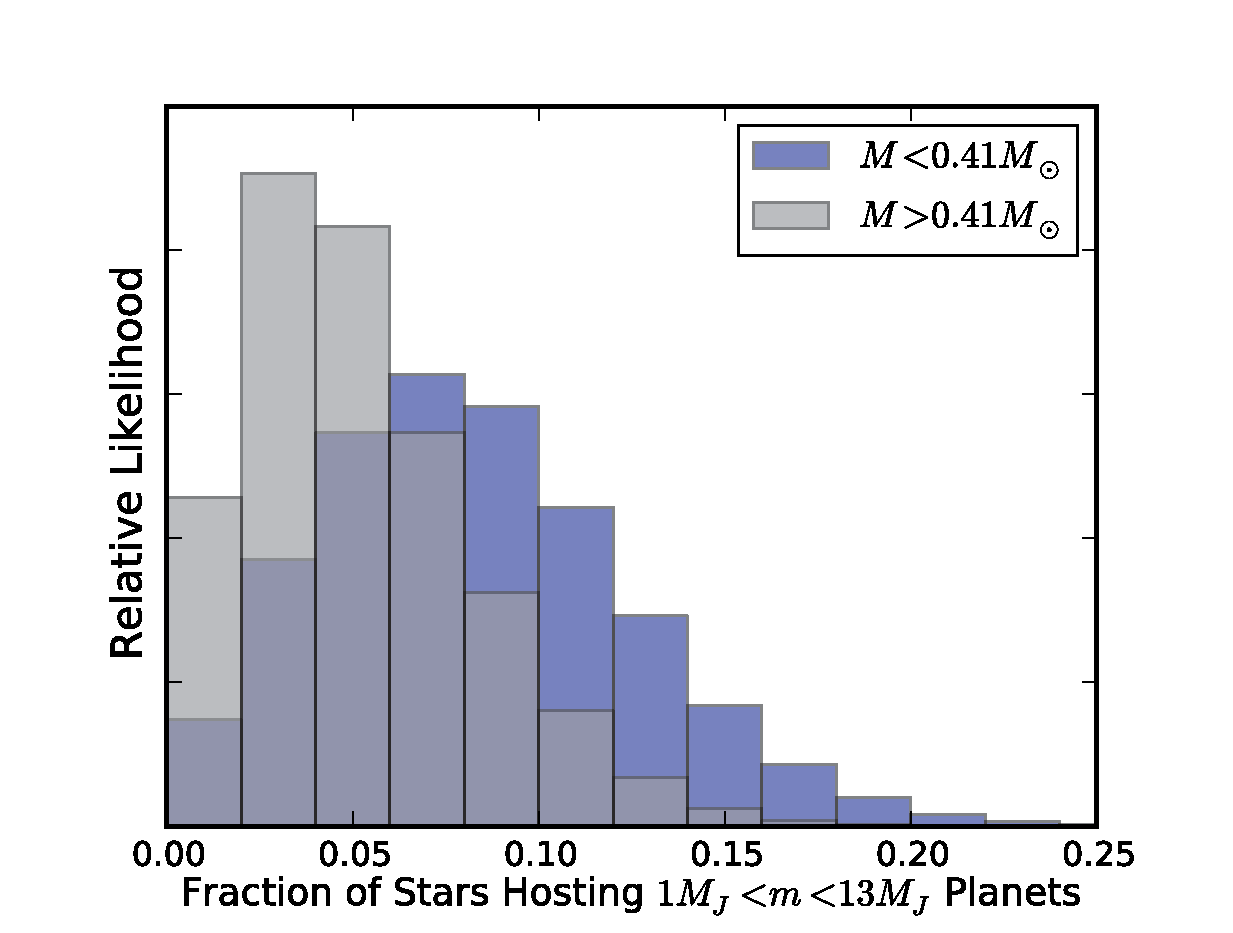
\includegraphics[width=0.75\textwidth]{chapter3/f10.eps}}
\caption[Posterior planet occurrence for a high-mass and low-mass
subpopulation of M dwarfs]{Planet occurrence for a low mass subsample (blue) and a high mass subsample (gray) of M dwarfs. Both subsets have nearly similar giant planet occurrence rates, suggesting planet occurrence may not depend strongly on stellar mass within the M spectral class. A larger sample is required to determine if the lack of difference in occurrence rates is astrophysical or statistical variance.
  }
\label{Mass}
\end{figure}



\subsection{Dependence on Metallicity}
\label{MetalDep}
Previous RV studies of giant planets have also found evidence for a correlation between planet occurrence and metallicity \citep{Fischer05, Johnson10a}. To test if this correlation holds for more distant planets, we again split our sample into two, using the same method from the previous section. In this case, we use [Fe/H] $= -0.10$, the sample median metallicity, as the dividing line for our subsamples. We assume all stars have metallicity uncertainties of 0.17 dex, consistent with the scatter expected from the \citet{Neves12} empirical relation. Again, we assume Gaussian errors to determine the probability each star is in a specific subsample. We then repeat our analysis on both groups.

\begin{figure}[htbp]
\centerline{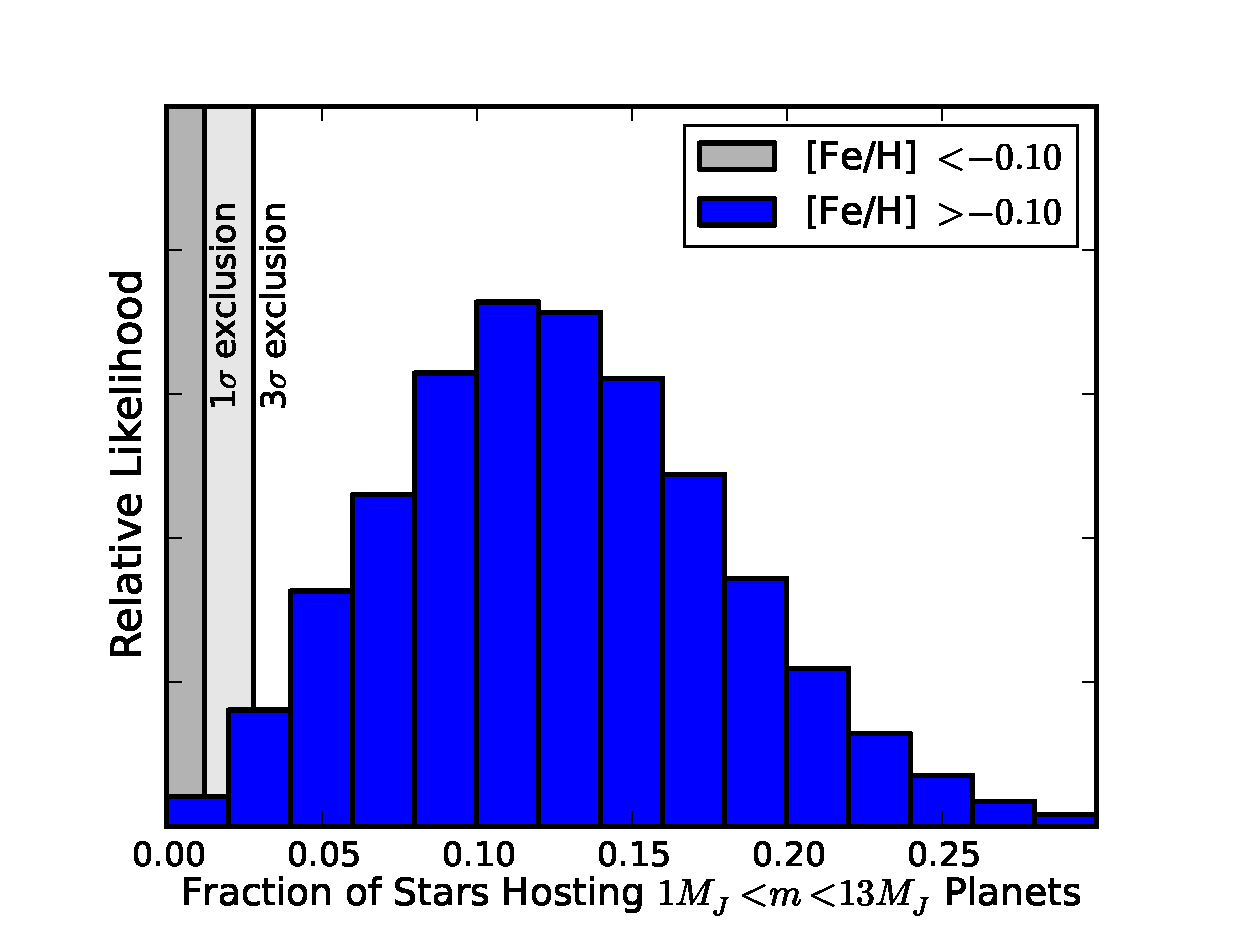
\includegraphics[width=0.75\textwidth]{chapter3/f11.eps}}
\caption[Posterior planet occurrence for a high-metallicity and low-metallicity
subpopulation of M dwarfs]{ Planet occurrence for a high metallicity subsample (blue) and 1$\sigma$ and 3$\sigma$ exclusion regions for a low metallicity subsample (gray) of M dwarfs. In the low metallicity subsample, we are able to rule out planet occurrence rates larger than 1.2\% at $1\sigma$ and 2.8\% at $3\sigma$, represented by the labeled vertical lines. The high metallicity sample has a significantly higher occurrence rate than the low metallicity sample, similar to the phenomenon observed for RV-detected planets at smaller separations. 
  }
\label{Metals}
\end{figure}
In the high-metallicity subsample, we find an occurrence rate such that $12.4 \pm 5.4\%$ of M-dwarfs host giant planets. In the low metallicity sample the occurrence rate drops to $0.96 \pm 0.51\%$. In Figure \ref{Metals} we plot a histogram of our posterior distribution of planet occurrence for our high-metallicity subsample. Vertical lines represent (from left to right) 1$\sigma$ and 3$\sigma$ upper limits on the planet occurrence rate for the low-metallicity subsample. From these distributions, the giant planet occurrence rate for metal-rich stars has only a $2.4\%$ probability of being lower than the $3\sigma$ upper limit on the planet occurrence rate for metal-poor stars. The difference between these subsamples may be suggestive of the same effect seen for RV-confirmed planets within 2.5 AU \citep{JohnsonApps09, KOI254}. 


An increase in the planet occurrence rate with metallicity for planets beyond a few AU may suggest giant planets in wide orbits are commonly formed by the same processes as the RV giant planet population. This study will be facilitated by the development of reliable spectroscopic metallicity measurements \citep{RA10}.


\subsection{The Stellar Mass-Metallicity Plane}
We can quantify our giant planet occurrence rate with respect to stellar mass and metallicity. Such an approach has been undertaken for planets with $a < 2.5$ AU orbiting stars of all spectral types previously \citep{Johnson10a}; we follow the techniques of these authors but confine ourselves to strictly giant planets in the range $0 < a < 20$ AU orbiting stars of the M-dwarf spectral class.

We assume that stellar mass and metallicity produce separate effects on the giant planet occurrence rate, so that the fraction of stars with planets as a function of mass and metallicity can be written as a double power-law,
\begin{equation}
f(M,F) = CM^a10^{bF},
\end{equation}
where $C$, $a$, and $b$ are constants, $M \equiv M/M\odot$, and $F \equiv$ [Fe/H].

In this analysis, we have a binary result: a star either has a giant planet, detectable as an RV acceleration or closed orbit, or it does not. Therefore, each of the $N$ stars in our sample represents a Bernoulli trial. Given $T$ total observed giant planets, if we assume the probability of a Doppler detection of a giant planet around any given star $i$ is $f(M_i, F_i)$, then by Bayes' theorem, the probability of a given model $X$ given our data $d$ is
\begin{equation}
P(X|d) \propto P(X) \prod_i^T f(M_i,F_i) \times \prod_j^{N-T} [1- f(M_j,F_j)].
\label{Likeli}
\end{equation}

Our measurements of stellar masses and metallicities are imperfect. Therefore, we treat the masses and metallicities of these stars as probability distributions. We consider each star's mass and metallicity distribution to be a two-dimensional Gaussian with mean {$M_i,F_i$} and standard deviation {$\sigma_{M,i},\sigma_{F,i}$ and call this term $p$. In this case, the predicted planet fraction for a star with mass $M_i$ and metallicity $F_i$ is
\begin{equation}
f(M_i,F_i) = \int \int p(M_i, F_i)f(M,F)dM dF.
\end{equation}
We can thus apply Eq. \ref{Likeli} with varying parameters, $X = {C, a, b}$, to maximize $\mathcal{L}$ conditioned on the data. We elect to use uniform priors, instead of applying the results of previous studies as a prior. \citet{Johnson10a} and \citet{Mortier13} study a sample of stars including all stellar types F to M, so their results may not represent our population well. More recent studies, such as \citet{Neves13}, are restricted to M-dwarfs. However, while their techniques are similar, they only attempt to constrain metallicity, implicitly assuming $a=0$. Additionally on of the three detected planets in their sample is a planet smaller than Jupiter around a metal-poor star. As our sample is limited to planets larger than Jupiter, the resultant distribution found by these authors may not be representative of the population of giant planets ($m > 1 M_J$).}

We find our giant planet fraction is described by the distribution function
\begin{equation}
f(M,F) = 0.039^{+0.056}_{-0.028} M^{0.8^{+1.1}_{-0.9}} 10^{(3.8 \pm 1.2)F}.
\end{equation}
The $1\sigma$ confidence interval for $C$ is highly skewed, while the other two parameters are approximately normally distributed. In Figure \ref{Covar}, we plot the marginal posterior probability distribution functions for each pair of parameters. Perhaps not surprisingly, we find a covariance between $C$ and $b$. Because our metallicity parameter $b$ is so steep, small changes in $b$ must cause changes in $C$ to keep the giant planet fraction consistent at a given metallicity.

\begin{figure}[htbp]
\centerline{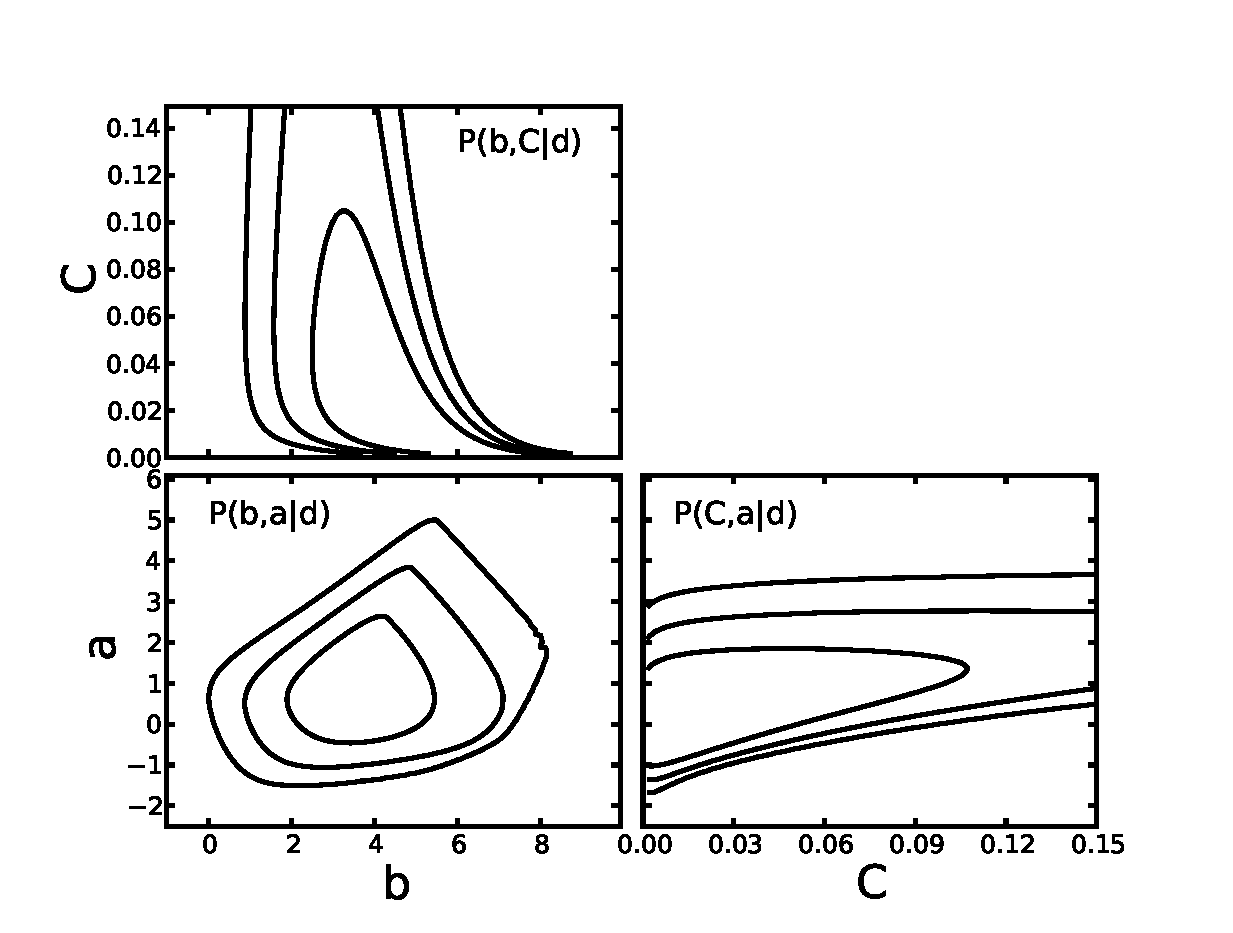
\includegraphics[width=0.75\textwidth]{chapter3/f12.eps}}
\caption[Marginal posterior distributions for the planet population model as a function of allowed power-law parameters]{Marginal posterior pdfs for the planet population model conditioned on our M-dwarf data. We find, as by other methods in previous sections, that giant planet occurrence is a strong function of stellar metallicity, but may not depend strongly on stellar mass inside of the M spectral class. 
  }
\label{Covar}
\end{figure}

Our results are steeper in $b$ than \citet{Neves13}, although the giant planet occurrence rates at [Fe/H] $\sim 0.1$ are consistent between the two studies. This is likely due to the inclusion of a planet with a minimum mass of 0.7 Jupiter masses in the ``Jovian'' sample of these authors. This planet orbits a star with a metallicity [Fe/H] $= -0.19 \pm 0.08$, flattening the distribution with metallicity. The fact remains that, while the metallicity distribution of field stars is centered near [Fe/H] $=0.0$ with a standard deviation of 0.13 dex, there are presently no giant planets orbiting M-dwarfs with measured metallicities smaller than +0.08 in either the HARPS or HIRES sample. The giant planet distribution function must therefore be a strong function of stellar metallicity. Moreover, it is essential to develop improved methods to measure metallicities of low-mass stars, such as the techniques developed by \citet{RojasAyala12} and \citet{Mann13a}.


\subsection{The Effect of Distant Binary Companions}

In the above analysis, we neglect binary stars where a test particle at 30 AU would be in an unstable orbit, but include 14 binaries at wider separations. Although these systems formally allow stable orbits, \citet{Kaib13} suggest these orbits can change significantly over time. Because the binary pair is weakly bound, interactions with the galactic tidal field or nearby passing stars can vary the binary orbit. The binary can then strongly perturb formerly stable planetary companions, potentially resulting in the ejection of planets from the system within 5 Gyr, our estimated age for the M-dwarfs in our sample. None of our 10 wide binary systems show evidence for an RV acceleration, providing weak but tantalizing evidence in favor of this theory. If we repeat our analysis but neglect these stars as potential hosting systems, we find that $7.4\% \pm 3.3\%$ of single stars host giant planets, compared to $6.5\% \pm 3.0\%$ of our full sample. With zero detections in a sample of 14 wide binaries, we can only place an upper limit of $f_{pl} \leq 0.20$ at $95\%$ confidence on the occurrence rate of giant planets in wide binary systems. With more observations of stars with wide binary companions, the occurrence rate of planets orbiting true field stars can be compared to the rate for wide binaries.



\subsection{Sensitivity to Power-Law Parameters}
\label{PL}
The result for $f_{pl}$ is dependent on the exact parameters of the planetary distribution function, as that function determines the number of missed (false negative) planets in our sample. To quantify the dependence of the planetary occurrence rate on our choice of $\alpha$ and $\beta$ we repeat our analysis over a grid of values for $\alpha$ and $\beta$. The giant planet occurrence rate as a function of these two parameters is shown in Figure \ref{AlpBetOcc}. We find that there is only a weak relation between $\alpha$ and $f_{pl}$ in the range $-2.0 < \alpha < 0.5$, where we might reasonably expect $\alpha$ to reside. $f_{pl}$ depends more strongly on $\beta$, but our overall result does not change by more than $1\sigma$ by selecting any $\beta$ in the range $-1.0 < \beta < 1.0$ for a given $\alpha$. Selecting any $\alpha$ or $\beta$ over this range affects our final result by less than a factor of two.

\begin{figure}[htbp]
\centerline{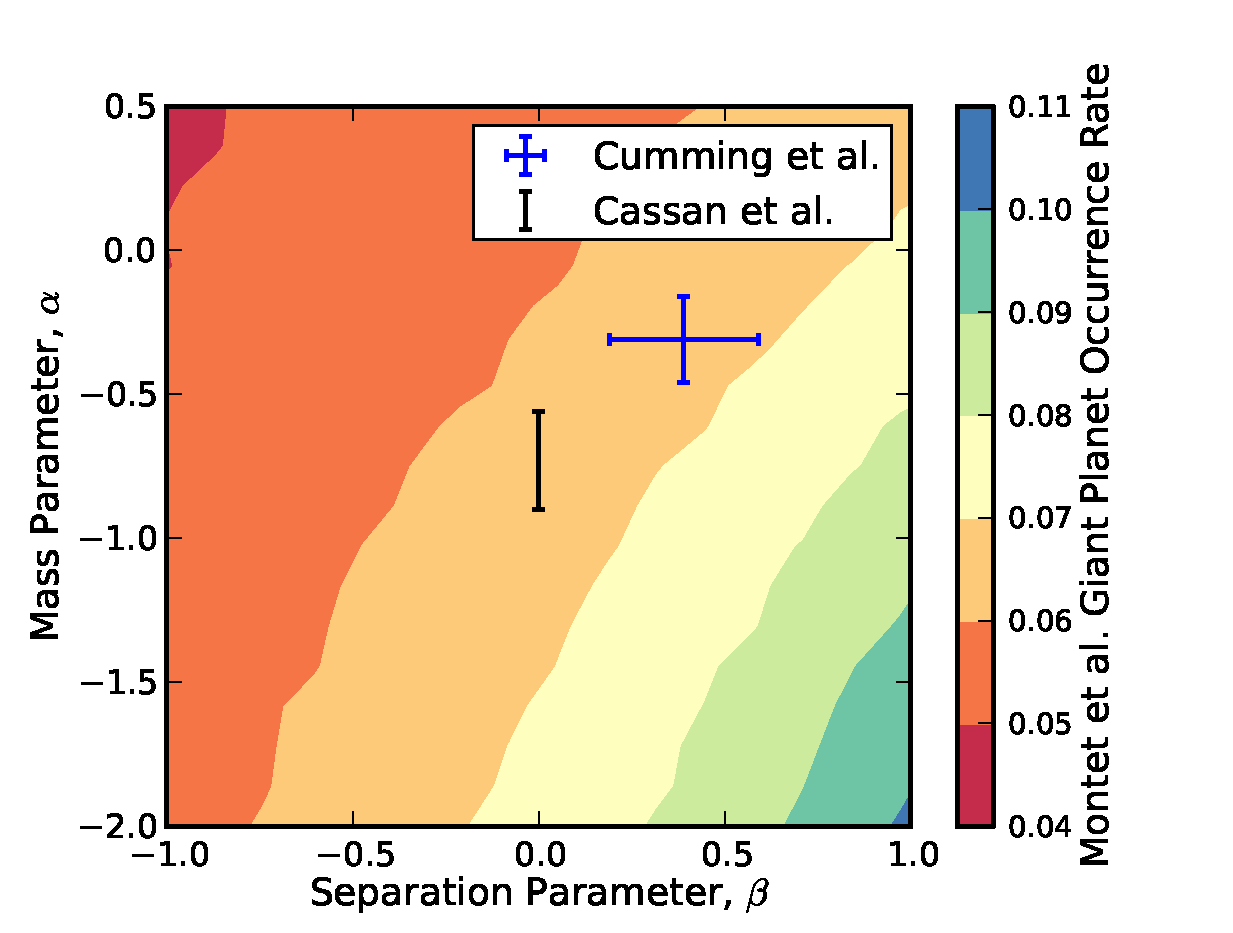
\includegraphics[width=0.75\textwidth]{chapter3/f13.eps}}
\caption[Calculated giant planet occurrence rate, $f_{pl}$, as a function of the mass parameter index $\alpha$ and separation parameter index $\beta$]{Calculated giant planet occurrence rate, $f_{pl}$, as a function of the mass parameter index $\alpha$ and separation parameter index $\beta$. There is not a strong dependence on $\alpha$ or $\beta$; selecting $\alpha < -1.0$ and $\beta > 0.5$ is required to affect our result at more than the $1\sigma$ level. Labeled points include the \citet{Cumming08} result for FGK stars, with $\alpha = -0.31 \pm 0.15$ and $\beta = 0.39 \pm 0.15$, and the microlensing result of \citet{Cassan12}, who find $\alpha = -0.73 \pm 0.17$ and assume $\beta \equiv 0$.
  }
\label{AlpBetOcc}
\end{figure}


From our sample of targets alone, we are unable to place constraints on acceptable values of $\alpha$ and $\beta$. To constrain $\alpha$ and $\beta$, the occurrence rate of giant planets at a given mass or separation is required. We have determined the bulk occurrence rate of planets, but cannot uniquely determine their properties. With continued observations, as our RV accelerations ``turn over'' and become closed orbits, we will be able to determine the exact locations of giant planets around M-dwarfs and constrain the power-law parameters. Alternatively, we can constrain $\alpha$ and $\beta$ by combining our results with those from microlensing observations.


\subsection{Comparison with Microlensing Results}
\label{muL}
 
In \textsection\ref{PL}, we showed that our bulk occurrence rate is not a strong function of $\alpha$ and $\beta$. However, the types and locations of our planets is a function of these parameters: if $\alpha$ is large, then most of our observed trends must be caused by large planets in wide orbits. Since microlensing results are most sensitive at projected separations corresponding to the Einstein radius, where $R_E \sim 3.5 \textrm{AU} (M_\star/M_\odot)^{1/2}$, we can compare our results to microlensing planet occurrence studies. As our results will only be consistent with microlensing estimates of the planet occurrence rate at the Einstein radius for specific values of $\alpha$ and $\beta$, comparisons between the two methods will enable us to constrain $\alpha$ and $\beta$. 

To compare the two sets of results, we assume the population of M-dwarfs observed by microlensing studies is similar to that targeted by RV surveys in the local neighborhood.  We find evidence for a correlation between giant planet frequency and metallicity in our sample, similar to that found by previous RV analyses of planets with $a < 2.5$ AU \citep{Fischer05, JohnsonApps09}. M-dwarfs studied by microlensing are at distances larger than 1 kpc and in the direction of the galactic bulge, along the galactic metallicity gradient \citep{Rolleston00}. Measurements of the metallicity of Cepheids suggest the iron content in the disk varies such that $d\textrm{[Fe/H]}/dr = -0.051 \pm 0.004$ dex kpc$^{-1}$ between 5 and 17 kpc from the galactic center \citep{Pedicelli09}. Thus, the microlensing M-dwarfs may be more metal-rich than stars in the local neighborhood, so $f_{pl}$ may be larger for the microlensing population than the RV population. Without spectra of galactic stellar planet-hosting lenses their true stellar properties are unknown. Programs dedicated to collecting spectra of galactic stellar planet-hosting lenses would greatly inform our knowledge of these stars and their planets.

If we assume the planet mass distribution function of \citet{Cumming08}, then from our analysis we would expect microlensing studies to measure a planet occurrence rate $f_{pl} = 0.056 \pm 0.023$ bound Jupiter-mass planets per star by analyzing signals from planets near the Einstein radius. \citet{Cassan12} claim an occurrence rate of $10^{-0.62\pm0.22}$ ($0.24^{+0.16}_{-0.10}$) Saturn-mass planets at this separation. If we scale this occurrence rate to Jupiter-mass planets following the mass index observed in microlensing studies, $\alpha = -0.73 \pm 0.17$, then the observed microlensing density of Jupiter mass planets would be $0.101 \pm 0.016$ planets per star, different from our expectation at $1.6\sigma$.  If (and only if) the two populations have intrinsically similar occurrence rates of giant planets, then the difference between the number of planets found must be due to a planet distribution different from the one used by \citet{Cumming08}. As the RV planet distribution was developed from an analysis of FGK stars, while the microlensing population generally consists of M dwarfs that may be preferentially metal-rich compared to stars in the local neighborhood, it may not be surprising if the RV planet population is intrinsically different from the microlensing planet population.

\subsubsection{Joint Constraints on $\alpha$}

We depart from our previously assumed values of $\alpha$ and $\beta$ to determine what values of $\alpha$ and $\beta$ satisfy both our observed RV accelerations and the results of \citet{Cassan12}. We assume the planet occurrence rate presented by \citet{Cassan12} is representative of the planet population at the Einstein radius. Moreover, we assume planet orbital semimajor axes are distributed uniformly in logarithmic space following \"Opik's Law ($\beta = 0$), as microlensing studies assume. This is slightly shallower than what is observed in the RV planet population ($\beta = 0.39 \pm 0.15$), but since the RV population of giant planets likely underwent considerable migration this may be a reasonable assumption. We then vary $\alpha$, and for each value determine the space density of planets at 2.5 AU. We then compare our expected result to the result from \citet{Cassan12}, which we scale to Jupiter-mass planets according to our $\alpha$ parameter. We finally require $\alpha < 0$: despite the uncertainties in this mass parameter, previous studies agree that around M dwarfs, small planets are more common than massive planets \citep{Swift13, Morton14}. 

We find microlensing results agree with our result for $f_{pl}$ when $\alpha = -0.94 \pm 0.56$ (Figure \ref{alphaopik}). This result is consistent with the best-fitting values for $\alpha$ found by \citet{Gould10} and \citet{Cassan12}. If we include the \citet{Cassan12} result as a prior in our analysis, we find $\alpha = -0.77 \pm 0.22$. However, while our result agree with microlensing studies, our result for $\alpha$ is different from the \citet{Cumming08} result for FGK stars at $1.1 \sigma$ and significantly different from the \citet{Bowler10} constraints for A stars, which rule out all $\alpha < 0.25$ with 90\% confidence and all $\alpha < 1.75$ with 50\% confidence. Since microlensing predicts a larger number of planets found at the Einstein radius relative to that expected by RV extrapolations, it is not surprising that we find a smaller value for $\alpha$ is required for our result to be consistent with the microlensing results: if the two populations are the same, there must be many low-mass giant planets below the simultaneous RV and imaging detectability limits than high-mass planets above the limits.

\begin{figure}[htbp]
\centerline{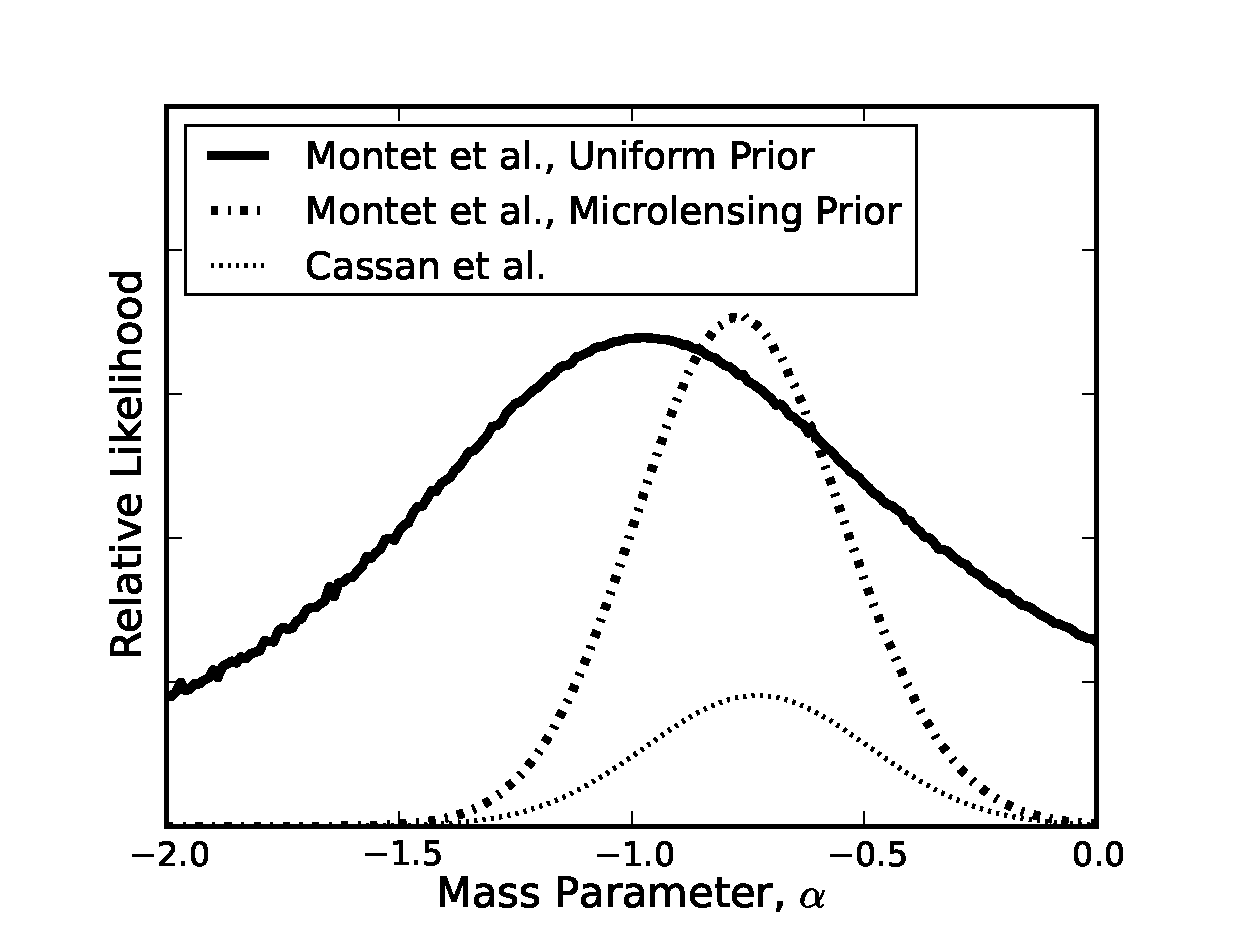
\includegraphics[width=0.75\textwidth]{chapter3/f14.eps}}
\caption[Relative likelihood values for the mass parameter $\alpha$, assuming the planets in our sample and microlensing systems are members of the same population]{Relative likelihood values for the mass parameter $\alpha$, assuming the planets in our sample and microlensing systems are members of the same population. We find a maximum likelihood value of $\alpha = -0.94 \pm 0.56$, consistent with values of $\alpha$ found from analyses of microlensing planets but steeper than previous RV results for FGK stars at $1.1 \sigma$. This result may suggest the planet distribution function is different for M stars as compared to higher mass stars. When we include the \citet{Cassan12} result as a prior on our measurement, we find $\alpha=-0.77 \pm 0.22$.
  }
\label{alphaopik}
\end{figure}

\subsubsection{Simultaneous Constraints on $\alpha$ and $\beta$}

We are not restricted to \"Opik's Law. We can allow both $\alpha$ and $\beta$ to vary, and compare the normalization of \citet{Cassan12} for Saturn-mass objects at 2.5 AU to our projected planet density at that mass and separation (Figure \ref{alphabeta}). Performing this exercise, we find the most acceptable values of $\alpha$ and $\beta$ are correlated approximately along the line $\alpha - \beta = -1$. That is, for every 1 dex increase in $\alpha$, $\beta$ must decrease by 1 dex to maintain a reasonable fit to both our result and the microlensing results. 

\begin{figure}[htbp]
\centerline{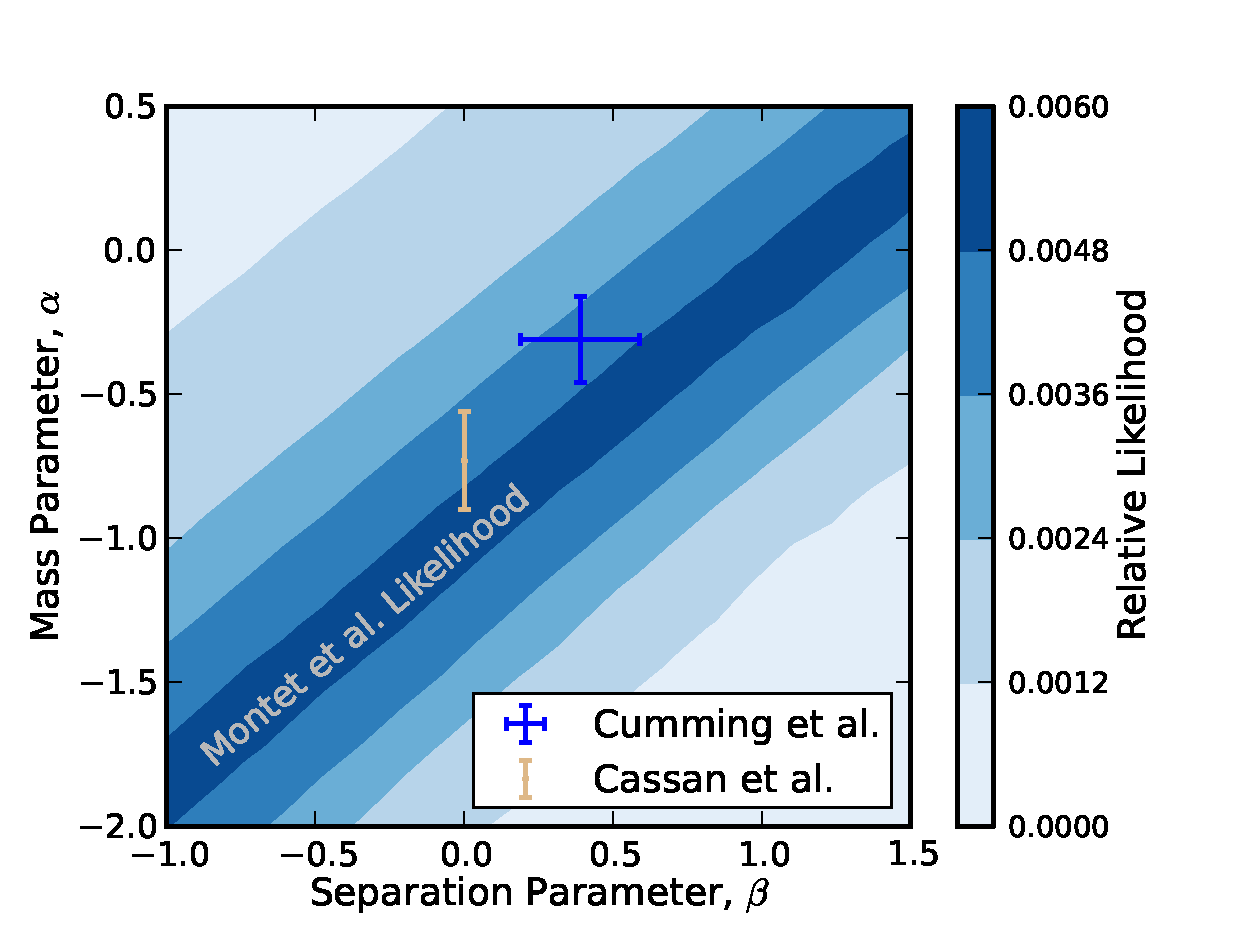
\includegraphics[width=0.75\textwidth]{chapter3/f15.eps}}
\caption[Relative likelihood values for the mass parameter $\alpha$ and separation parameter $\beta$]{Relative likelihood values for the mass parameter $\alpha$ and separation parameter $\beta$. There is a maximum likelihood contour approximately along the line $\alpha - \beta = -1$, suggesting a relationship between the two parameters required to fit both our result and the microlensing results, assuming the local planets in our sample and microlensing systems are members of the same population. Points included in the plot are the \citet{Cumming08} RV result (blue) and the \citet{Cassan12} microlensing result (cyan), the latter of which assumes an \"Opik's Law value of $\beta = 0$. The small discrepancy between our result and the \citet{Cumming08} result may suggest the planet distribution function may differ between M-dwarfs and FGK stars.
}
\label{alphabeta}
\end{figure}

\subsubsection{A Model-Independent $f_{pl}$}
We can apply these relative likelihood values as priors to the occurrence rate as a function of $\alpha$ and $\beta$ shown in Figure \ref{AlpBetOcc} to determine an occurrence rate independent of our choices of $\alpha$ and $\beta$, but dependent on the RV and microlensing stars both being representative of similar populations. We assume our separation parameter must be in the range $-1.0 < \beta < 1.0$, consistent with the assumptions from previous microlensing studies, and allow our mass parameter to be any value subject to the constraints of Figure \ref{alphabeta}. By weighting our occurrence rates found in \textsection\ref{PL} in this manner, we find a most likely occurrence rate of $7.2 \pm 3.1\%$, consistent with that found by assuming the power-law distribution of \citet{Cumming08}. As the measured planet frequency depends on the distribution function parameters, an improved value of the planet occurrence rate, either by this method, microlensing, or through astrometry measured by \textit{Gaia} \citep{Casertano08}, will provide immediate constraints on the distribution function of giant planets. Similarly, improved constraints on the distribution parameters will enable an immediate improvement of the determination of the giant planet occurrence rate.

The \citet{Cumming08} power-law parameters $\alpha$ and $\beta$ are less consistent with our results. This may suggest the planet distribution function around FGK stars is systematically different from the planet distribution function around M-dwarfs. As \citet{Bowler10} find an even larger value for $\alpha$ in their study of retired A stars (excluding all $\alpha < 0$), which matches comparison studies between RV surveys and high-contrast imaging searches \citep{Crepp11}, this possibility is certainly plausible. With additional M-dwarfs targeted by a combination of RV observations with longer time baselines and high-contrast imaging to improve the estimate of the occurrence rate, we will be able to directly probe this possibility.




\section{Summary and Conclusion}
\label{SC}
We have analyzed a collection of 111 nearby M-dwarfs observed in RV surveys with a median time baseline of 11.8 years in a search for long-term RV accelerations. We have developed a new technique to determine the incidence of giant planets in which we target systems with such accelerations using adaptive optics imaging to ``peer beyond the horizon'' set by Doppler time baselines. With a relatively short exposure image using the Keck AO system, we can eliminate the possibility of binary stellar companions and massive brown dwarfs. We conclude with high statistical confidence that accelerations without a directly imaged companion are likely caused by a planet in a wide orbit. 

Accounting for false positive and false negative rates, we find that $6.5 \pm 3.0\%$ of M-dwarfs host a giant planet with mass $1 < m / M_J < 13 $ and semimajor axis $0 < a < 20$ AU, assuming such planets are distributed following the power-law parameters estimated by \citet{Cumming08}. The exact integrated planet occurrence rate does not depend strongly on the distribution function parameters chosen. We find evidence for a correlation between giant planet frequency and stellar metallicity, similar to that observed in the RV-detected planet population. Additional follow-up work confirming this result would suggest giant planets in wide orbits may form in the same way as the RV-detected giant planets. Observations of more stars are needed to determine if a correlation exists between planet occurrence at wide separations and stellar mass inside of the M-dwarf spectral class. 

Our overall occurrence rate is consistent with what might be expected based on the results of microlensing planet search surveys. However, if the giant planet distribution is given as a double power law similar to that found by \citet{Cumming08}, such that $d^2N \propto M^\alpha a^\beta d\ln M d\ln a$, with $\alpha = -0.31 \pm 0.20$ and $\beta = 0.39 \pm 0.15$, where $\alpha$ and $\beta$ are planet distribution power-law indices defined in Eq. \ref{DPL}, then microlensing studies overestimate the giant planet occurrence rate. From our bulk occurrence rate, we determine an expected planet detection rate for microlensing studies which depends on our chosen planet distribution function. By assuming an \"Opik's Law distribution (i.e., flat in $\log a$), the microlensing planet occurrence rate is consistent with our result if the planet population is represented by the power-law $dN \propto m^{-0.94 \pm 0.56} d\log m$. This value for $\alpha$ is consistent with previous M-dwarf studies conducted by microlensing planet search teams \citep{Gould10, Cassan12}. We also find other non-\"Opik distributions can be chosen to simultaneously explain our results and the microlensing results; these fall approximately on the line $\alpha - \beta = -1$. Moreover, an improved estimate of the giant planet occurrence rate, as measured by \textit{Gaia}, can be combined with our results to provide enhanced constraints on $\alpha$ and $\beta$.  

Our knowledge of planets around M-dwarfs has significantly improved in the last few years thanks to both targeted RV searches and high contrast imaging campaigns \citep{Apps10, Bowler12a}. As such surveys continue, they will begin to confirm and characterize planets in wider orbits, pushing into the domain currently only studied by microlensing studies. To directly compare these populations, understanding the properties of host stars to planets found by microlensing will be extremely important; when possible, every effort should be made to collect spectroscopic followup data on microlensing events to determine the physical properties of lens host stars to better understand both the planet population around M-dwarfs and how it changes across the galaxy.

The method developed in this paper can be extended to higher-mass stars with little difficulty. For example, a large sample of K-dwarfs has been observed by the CPS collaboration. This sample is larger, has more observations, and exhibits less astrophysical jitter than our M-dwarf sample; all of these factors improve our ability to detect RV accelerations. However, the stars are more luminous and on average more distant, complicating adaptive optics searches. Care must be taken to ensure low-mass stellar companions are accounted for, as adaptive optics imaging may not be sensitive to all M-dwarf companions to K-dwarfs without longer observations or the use of ADI. In the future, we intend to apply this technique to the CPS K-dwarfs to determine the planet occurrence rate around higher mass stars and compare to the M-dwarfs.

\begin{landscape}
{\footnotesize
\begin{longtable}{l|cccccccccccc} 
\hline
Star & RA & Dec & Mass ($M_\odot$) & [Fe/H] & Spectral Type & $V$ & $V$ Source & d (pc) \\
\hline
    Hip 428 & 00:05:10.9 & +45:47:11.6 & 0.53 & -0.07 & M1 &  9.93 & \citet{Gliese91} & 11.25  \\ 
    HD 225213 & 00:05:24.4 & -37:21:26.5 & 0.39 & -0.42 & M1.5 &  8.57 & \citet{Koen10} &  4.34  \\ 
   Hip 1734 & 00:21:56.0 & -31:24:21.8 & 0.55 & 0.09 & M1.5 &  11.1 & \citet{Koen10} & 17.98    \\ 
      Gl 26 & 00:38:59.0 & +30:36:58.5 & 0.43 & 0.02 & M2.5 & 11.2 & \citet{Hog00} &  12.6  \\ 
   Hip 3143 & 00:39:58.8 & -44:15:11.6 & 0.55 & -0.09 & M0.5 &  11.4 & \citet{Koen10} & 23.99 \\ 
      Gl 48 & 01:02:32.2 & +71:40:47.3 & 0.48 & 0.06 & M3 & 10.0 & \citet{Hog00} &  8.24   \\ 
      Gl 49 & 01:02:38.9 & +62:20:42.2 & 0.58 & 0.06 & M1.5 & 9.56 & \citet{Hog00} & 9.96    \\ 
   Hip 5643 & 01:12:30.6 & -16.59.56.3 & 0.13 & -0.43 & M4.5 & 12.1 & \citet{Koen10} & 3.69  \\
   Hip 8051 & 01:43:20.2 & +04:19:18.0 & 0.41 & -0.16 & M2 &  10.9 & \citet{Koen10} & 11.41  \\ 
   Gl 83.1 & 02:00:13.0 & +13:03:07.0 & 0.15 & -0.31 & M4.5 & 12.3 & \citet{Landolt92} & 4.50    \\
  G244-047 & 02:01:35.3 & +63:46:12.1 & 0.48 & 0.07 & M3 & 11.0 & \citet{Hog00} & 12.76    \\ 
      Gl 87 & 02:01:35.3 & +63:46:12.1 & 0.45 & -0.32 & M1.5 & 10.0 & \citet{Koen10} & 10.41 \\ 
  Hip 11048 & 02:22:14.6 & +47:52:48.1 & 0.62 & -0.08 & M0.5 & 9.41 & \citet{Gliese91} & 11.94   \\ 
    Gl 105B & 02:36:15.3 & +06:52:19.1 & 0.27 & -0.10 & M4 & 11.6 & \citet{Jenkins09} & 7.73 \\ 
     Gl 109 & 02:44:15.6 & +25:31:24.1 & 0.35 & -0.18 & M3 & 10.6 & \citet{Koen10} &  7.51    \\ 
  Hip 21556 & 04:37:42.9 & -11:02:19.9 & 0.48 & -0.11 & M1.5 &  10.3 & \citet{Koen10} & 11.10    \\ 
  Gl 179 & 04:52:05.7 & +06:28:35.6 & 0.36 & 0.13 & M3.5 &  12.0 & \citet{Koen10} & 12.29  \\
  Hip 22762 & 04:59:50.0 & -17:46:24.3 & 0.42 & -0.20 & M2 & 10.9 & \citet{Koen10} & 12.12  \\ 
  Hip 23512 & 05:03:20.1 & -17:22:24.7 & 0.27 & -0.25 & M3 & 11.7 & \citet{Koen10} & 9.21   \\
    HD 33793 & 05:11:40.6 & -45:01:06.3 & 0.27 & -0.81 & M1 &  8.85 & \citet{Koen10} &  3.91   \\ 
 Hip 24284 & 05:12:42.2 & +19.39.56.4 & 0.45 & -0.16 & M2 & 10.7 & \citet{Koen10} & 12.29  \\ 
    HD 36395 & 05:31:27.4 & -03:40:38.0 &  0.60 & -0.05 & M1.5 &  7.92 & \citet{Koen10} & 5.66  \\ 
  G097-054 & 05:34:52.1 & +13:52:47.2 & 0.37 & 0.05 & M3.5 &  11.9  & \citet{Kharchenko01} &  12.39  \\ 
  HD 233153 & 05:41:30.7 & +53:29:23.3 & 0.60 & 0.05 & M0.5 &  9.75 & \citet{Gliese91} & 12.44  \\
  Hip 26857 & 05:42:09.3 & +12.29:21.6 & 0.22 & -0.24 & M4 & 11.5 & \citet{Landolt92} & 5.83    \\
   G192-13 & 06:01:11.1 & +59:35:50.8 &  0.27 & -0.11 & M3.5 &  11.7 & \citet{VanAltena95} &  7.93   \\ 
  Hip 29052 & 06:07:43.7 & -25:44:41.5 & 0.30 & -0.22 & M4 & 11.9 & \citet{Koen10} & 11.35   \\ 
     Gl 226 & 06:10:19.8 & +82.06:24.3 & 0.41 & -0.14 & M2 & 10.5 & \citet{Gliese91} & 9.37   \\ 
     Gl 229B & 06:10:34.6 & -21:51:52.7 & 0.58 & -0.07 & M1 & 8.13 & \citet{Koen10} &  5.75  \\
    Gl 250B & 06:52:18.1 & -05:11:24.2 & 0.45 & -0.12 & M2 & 10.1 & \citet{Gliese91}  &  8.71  \\
    HD 265866 & 06:54:49.0 & +33:16:05.4 & 0.35 & -0.03 & M3 & 10.11 & \citet{Hog00} &  5.59  \\ 
     Gl 273 & 07:27:24.5 & +05:13:32.8 & 0.29 & -0.07 & M3.5 & 9.87 & \citet{Koen10} &  3.80   \\ 
  Hip 36338 & 07:28:45.4 & -03:17:53.4 & 0.40 & 0.03 & M3 & 11.4 & \citet{Koen10} & 12.29 \\ 
  Hip 36834 & 07:34:27.4 & +62:56:29.4 & 0.40 & -0.50 & M0.5 & 10.4 & \citet{Hog00} & 11.47   \\ 
 Hip 37217 & 07:38:41.0 & -21:13:28.5 & 0.29 & -0.27 & M3 & 11.7 & \citet{Koen10} & 10.60   \\
  Hip 37766 & 07:44:40.2 & +03:33:08.8 & 0.31 & 0.27 & M4.5 & 11.2 & \citet{Koen10} & 5.96  \\
    GJ 2066 & 08:16:08.0 & +01:18:09.3 & 0.46 & -0.10 & M2 & 10.1 & \citet{Koen10} & 9.12   \\ 
     Gl 317 & 08:40:59.2 & -23:27:23.3 & 0.43 & 0.20 & M3.5 &  12.0 & \citet{VanAltena95} &  15.31   \\ 
    HD 75732B & 08:52:40.8 & +28:18:59.0 & 0.27 & 0.15 & M4 & 13.1 & \citet{Gliese91} & 13.02  \\
  Hip 46655 & 09:30:44.6 & +00:19:21.6 & 0.29 & -0.17 & M3.5 & 11.7 & \citet{Koen10} & 9.67  \\
  Hip 46769 & 09:31:56.3 & +36.19:12.8 & 0.53 & -0.27 & M0 & 10.1 & \citet{Hog00} & 13.91   \\ 
     Gl 357 & 09:36:01.6 & -21:39:38.9 & 0.33 & -0.31 & M2.5 &  10.9 & \citet{Koen10} &  9.02  \\ 
  Hip 47513 & 09:41:10.4 & +13:12:34.4 &  0.48 & -0.12 & M1.5 & 10.4 & \citet{Koen10} & 11.26  \\ 
  Hip 47650 & 09:42:51.7 & +70:02:21.9 & 0.41 & 0.13 & M3 & 11.4 & \citet{Hog00} & 11.35    \\
  Hip 48714 & 09:56:08.7 & +62:47:18.5 & 0.64 & -0.03 & M0 &  9.00 & \citet{Gliese91} & 10.56   \\ 
     Gl 382 & 10:12:17.7 & -03:44:44.4 & 0.54 & 0.02 & M1.5 &  9.26 & \citet{Koen10} & 7.87  \\  
     Gl 388 & 10:19:36.3 & +19:52:10.1 & 0.41 & 0.10 & M3.5 & 9.46 & \citet{Hog00} & 4.69  \\
  Hip 51007 & 10:25:10.8 & -10:13:43.3 & 0.54 & -0.07 & M1 & 10.1 & \citet{Koen10} & 12.35 \\ 
     Gl 393 & 10:28:55.6 & +00:50:27.6 & 0.44 & -0.14 & M2 & 9.65 & \citet{Landolt09} &  7.07   \\
 Hip 53020 & 10:50:52.0 & +06:48:29.2 & 0.26 & 0.00 & M4 & 11.7 & \citet{Landolt92} & 6.76  \\
  Gl 406 & 10:56:28.9 & +07:00:52.8 & 0.10 & 0.22 & M5.5 & 13.5 & \citet{Landolt92} & 2.39   \\
     Gl 408 & 11:00:04.3 & +22:49:58.6 &  0.38 & -0.15 & M2.5 & 10.0 & \citet{Koen10} &  6.66 \\ 
    HD 95650 & 11:02:38.3 & +21:58:01.7 &  0.59 & -0.10 & M0 & 9.57 & \citet{Koen10} & 11.77   \\ 
    HD 95735 & 11:03:20.2 & +35.58:11.6 & 0.39 & -0.32 & M2 & 7.52 & \citet{Oja85} &  2.55  \\ 
  Hip 54532 & 11:09:31:3 & -24:35:55.1 & 0.46 & -0.08 & M2 & 10.4 & \citet{Koen10} & 10.75  \\ 
   HD 97101B & 11:11:01.9 & +30:26:44.4 & 0.58 & 0.52 & M1.5 & 10.7 & \citet{Hog00} & 11.87 \\
  Hip 55360 & 11:20:04.8 & +65:50:47.3 & 0.49 & -0.35 & M0 &  9.30 & \citet{Hog00} & 8.92  \\ 
     Gl 433 & 11:35:26.9 & -32:32:23.9 & 0.47 & -0.15 & M1.5 &  9.81 & \citet{Koen10} &  8.88    \\ 
  Hip 57050 & 11:41:44.6 & +42:45:07.1 & 0.35 & 0.08 & M4 & 11.9 & \citet{Kharchenko01} & 11.10  \\ 
  Gl 436 & 11:42:11.2 & +26:42:22.6 &  0.44 & -0.03 & M2.5 & 10.6 & \citet{Hog00} & 10.14   \\ 
     Gl 445 & 11:47:41.4 & +78:41:28.2 & 0.25 & -0.27 & M3.5 & 10.8 & \citet{Hog00} &  5.35  \\ 
 Hip 57548 & 11:47:44.4 & +00:48:16.4 & 0.17 & -0.23 & M4 & 11.1 & \citet{Landolt92} & 3.36 \\
     Gl 450 & 11:51:07.3 & +35:16:19.3 & 0.46 & -0.21 & M1 & 9.72 & \citet{Hog00} &  8.59  \\ 
  Hip 59406 & 12:11:11.8 & -19:57:38.1 & 0.35 & -0.13 & M3 & 11.7 & \citet{Koen10} & 12.59 \\ 
  Hip 59406b & 12:11:17.0 & -19:58:21.4 & 0.25 & -0.25 & M4 & 12.6 & \citet{Gliese91}  & 12.59  \\
  Hip 60559 & 12:24:52.5 & -18:14:32.2 & 0.26 & -0.56 & M4 & 11.3 & \citet{Koen10} & 8.85  \\
     Gl 486 & 12:47:56.6 & +09:45:05.0 & 0.32 & 0.01 & M3.5 &  11.4 & \citet{Koen10} &  8.37  \\ 
  Hip 63510 & 13:00:46.6 & +12:22:36.6 & 0.594 & 0.04 & M0.5 & 9.76 & \citet{Koen10} & 11.4  \\ 
     Gl 514 & 13:29:59.8 & +10:22:37.8 & 0.53 & -0.15 & M0.5 & 9.03 & \citet{Koen10} &  7.66  \\ 
   HD 119850 & 13:45:43.8 & +14:53:29.5 & 0.50 & -0.16 & M1.5 & 8.50 & \citet{VanBelle09} &  5.39 \\
  Hip 67164 & 13:45:50:7 & -17:58:05.6 & 0.31 & -0.06 & M3.5 & 11.9 & \citet{Koen10} & 10.24  \\ 
   HD 122303 & 14:01:03.2 & -02:39:17.5 & 0.52 & -0.16 & M1 & 9.71 & \citet{Koen10} & 10.03    \\ 
  Hip 70865 & 14:29:29.7 & +15:31:57.5 & 0.52 & 0.00 & M2 & 10.7 & \citet{Koen10} & 14.00 \\
  Hip 70975 & 14:31:01.2 & -12:17:45.9 & 0.32 & -0.05 & M3.5 & 11.9 & \citet{Koen10} & 10.82  \\ 
  Hip 71253 & 14:34:16.8 & -12:31:10.4 & 0.28 & 0.11 & M4 &  11.3 & \citet{Koen10} &  6.06 \\ 
  Hip 71898 & 14:42:21.6 & +66:03:20.9 & 0.361 & -0.35 & M3 & 10.8 & \citet{Hog00} &  9.87  \\ 
  Gl 569A & 14:54:29.2 & +16:06:03.8 & 0.48 & -0.03 & M2.5 & 10.2 & \citet{Koen10} & 9.65  \\
  Gl 581 & 15:19:27.5 & -07:43:19.4 & 0.30 & -0.18 & M3 & 10.6 & \citet{Hog00} & 6.21 \\
   HD 147379B & 16:16:45.3 & +67:15:22.5 & 0.47 & 0.09 & M3 & 10.7 & \citet{Gliese91} & 10.74 \\
     Gl 625 & 16:25:24.6 & +54:18:14.7 & 0.32 & -0.39 & M1.5 & 10.2 & \citet{Hog00} &  6.52  \\ 
  Gl 649 & 16:58:08.9 & +25:44:39.0 & 0.54 & -0.10 & M1 & 9.66 & \citet{Hog00} & 10.34  \\
  Hip 83762 & 17:07:07.5 & +21:33:14.5 & 0.38 & -0.10 & M3 & 11.7 & \citet{Koen10} & 13.4   \\
  Hip 84099 & 17:11:34.7 & +38:26:33.9 & 0.38 & -0.05 & M3.5 & 11.5 & \citet{Hog00} & 12.00   \\ 
  Hip 84790 & 17:19:52.7 & +41:42:49.7 & 0.37 & -0.21 & M2.5 & 11.4 & \citet{Gliese91} & 12.38  \\ 
     Gl 687 & 17:36:25.9 & +68:20:20.9 & 0.40 & -0.06 & M3 & 9.15 & \citet{Hog00} & 4.53  \\
     Gl 686 & 17:37:53.3 & +18:35:30.2 & 0.44 & -0.31 & M1 & 9.58 & \citet{Koen10} & 8.09   \\ 
     Gl 694 & 17:43:56.0 & +43:22:43.0 & 0.44 & -0.02 & M2.5 & 10.5 & \citet{Hog00} &  9.48   \\ 
     Gl 699 & 17:57:48.5 & +04:41:36.2 & 0.16 & -0.61 & M4 & 9.51 & \citet{Koen10} & 1.82   \\ 
   HD 165222 & 18:05:07.6 & -03:01:52.8 & 0.48 & -0.22 & M1 &  9.36 & \citet{Koen10} &  7.76 \\ 
 G205-028 & 18:31:58.4 & +40:41:10.4 & 0.31 & -0.14 & M3.5 & 12.0 & \citet{Gliese91} & 11.9 \\
    GJ 4063 & 18:34:36.6 & +40:07:26.4 & 0.19 & -0.61 & M3.5 & 11.8 & \citet{Hog00} &  7.25    \\ 
  Hip 91699 & 18:41:59.0 & +31:49:49.8 & 0.37 & -0.13 & M3 & 11.3 & \citet{Kharchenko01} & 11.45  \\
  Hip 92403 & 18:49:49.4 & -23:50:10.4 & 0.17 & -0.43 & M3.5 & 10.5 & \citet{Koen10} & 2.97  \\
    Gl 745A & 19:07:05.6 & +20:53:17.0 & 0.30 & -0.48 & M1.5 & 10.8 & \citet{Koen10} &  8.51  \\
    Gl 745B & 19:07:13.2 & +20:52:37.2 & 0.31 & -0.45 & M1.5 & 10.7 & \citet{Koen10} & 8.75  \\
 G207-019 & 19:08:30.0 & +32:16:52.0 & 0.34 & -0.10 & M3 & 11.8 & \citet{Kharchenko01} & 12.39   \\
   HD 180617 & 19:16:55.3 & +05:10:08.1 & 0.48 & 0.02 & M2.5 &  9.12 & \citet{Koen10} &  5.87  \\
     Gl 793 & 20:30:32.0 & +65:26:58.4 & 0.38 & -0.03 & M2.5 & 10.7 & \citet{Hog00} &  8.00  \\ 
     Gl 806 & 20:45:04.1 & +44:29.56.7 & 0.44 & -0.16 & M1.5 & 10.8 & \citet{Hog00} & 12.32    \\ 
 Hip 103039 & 20:52:33.0 & -16:58:29.0 & 0.23 & -0.10 & M4 & 11.4 & \citet{Koen10} & 5.71  \\
   HD 199305 & 20:53:19.8 & +62:09:15.8 &  0.58 & -0.02 & M0.5 &  8.60 & \citet{Hog00} &  7.05   \\ 
 Hip 104432 & 21:09:17.4 & -13:18:09.0 & 0.36 & -0.51 & M1 & 10.9 & \citet{Landolt09} & 12.17   \\ 
   HD 209290 & 22:02:10.3 & +01:24:00.8 & 0.60 & -0.10 & M0 & 9.15 & \citet{Koen10} & 10.24  \\ 
 Gl 849 & 22:09:40.3 & -04:38:26.6 & 0.49 & 0.22 & M3.5 & 10.4 & \citet{Koen10} &  9.10  \\
 Hip 109555 & 22:11:30.1 & +18:25:34.3 & 0.55 & 0.13 & M2 & 10.2 & \citet{Koen10} & 11.62   \\
     Gl 876 & 22:53:16.7 & -14:15:49.3 & 0.34 & 0.13 & M4 & 10.2 & \citet{Landolt09} &  4.69 \\
   HD 216899 & 22:56:34.8 & +16:33:12.4 & 0.58 & 0.03 & M1.5 & 8.64 & \citet{Koen10} & 6.84 \\
   HD 217987 & 23:05:52.0 & -35:51:11.0 & 0.47 & -0.33 & M0.5 & 7.34 & \citet{Gliese91} & 3.28  \\ 
 Hip 114411 & 23:10:15.7 & -25:55:52.7 & 0.46 & -0.13 & M2 & 11.3 & \citet{Koen10} & 16.08   \\ 
 Hip 115332 & 23:21:37.4 & +17:17:25.4 & 0.40 & 0.27 & M4 & 11.7 & \citet{Koen10} & 10.99  \\ 
 Hip 115562 & 23:24:30.5 & +57:51:15.5 & 0.59 & 0.08 &  M1 & 10.0 & \citet{Gliese91} & 12.96\\ 
 Gl 905 & 23:41:55.0 & +44:10:40.8 & 0.14 & 0.05 & M5 & 12.3 & \citet{Jenkins09} & 3.16 \\
     Gl 908 & 23:49:12.5 & +02:24:04.4 & 0.42 & -0.39 & M1 & 8.99 & \citet{Landolt09} &  5.98\\
\hline
\caption[M-dwarf stars analyzed in this study]{M-dwarf stars analyzed in this study. Metallicity uncertainties are taken to be 0.17 dex, while mass uncertainties are taken as $10\%$, following the method of \citet{Delfosse00}}
\label{T1}
\end{longtable}
}
\end{landscape}

\clearpage

\begin{landscape}
{\footnotesize
\begin{longtable}{l|ccccccc} 
\hline
Star & N$_\textrm{obs}$ & Baseline (yr) & 
Med. $\sigma_{\gamma}$ (m s$^{-1}$) & Jitter (m s$^{-1}$) & RMS (m s$^{-1}$) & RV Planets & Binary Companion \\
     \hline
Hip 428 &  41 &  12.2 &   1.6 &   4.2 &   4.8 & 0 & K6 \citep{Bidelman54}  \\ 
HD 225213  &  67 &   9.9 &   1.1 &   3.2 &   3.1 & 0 & -  \\ 
Hip 1734  &   8 &   8.1 &   2.6 &   4.7 &   7.6 & 0 & -  \\ 
Gl 26  &  40 &  11.6 &   2.8 &   2.9 &   7.7 & 0 & -  \\ 
Hip 3143  &   8 &   9.8 &   5.6 &   2.6 &  11.6 & 0 & -  \\ 
Gl 48  &  41 &  15.2 &   1.3 &   2.5 &   3.5 & 0 & -  \\ 
Gl 49  &  22 &  14.2 &   1.4 &   7.9 &   5.0 & 0 & -  \\ 
Hip 5643  &  15 &   7.1 &   3.4 &  13.2 &   7.8 & 0 & -  \\ 
Hip 8051  &  33 &  12.7 &   1.5 &   3.0 &   5.0 & 0 & -  \\ 
Gl 83.1  &  21 &   8.2 &   3.3 &  12.5 &  20.2 & 0 & -  \\ 
G244-047  &  10 &   7.5 &   2.8 &   3.6 &   4.0 & 0 & -  \\ 
Gl 87 &  62 &  13.0 &   1.3 &   2.5 &   7.4 & 0 & -  \\ 
Hip 11048  &  44 &  12.6 &   1.1 &   4.8 &   5.4 & 0 & -  \\ 
Gl 105B &  12 &   9.1 &   2.7 &   3.7 &  13.0 & 0 & K3 \citep{Gray06}  \\ 
Gl 109  &  32 &  13.1 &   1.4 &   2.8 &   4.4 & 0 & -  \\ 
Hip 21556  &  31 &  12.7 &   1.3 &   2.5 &   4.3 & 0 & -  \\ 
Gl 179 &  42 &  12.2 &   2.5 &   4.4 &  19.7 & 1 & -  \\ 
Hip 22762  &  39 &  12.6 &   1.6 &   2.7 &   4.6 & 0 & -  \\ 
Hip 23512  &  11 &   6.7 &   4.1 &   5.0 &   6.7 & 0 & -  \\ 
HD 33793  &  36 &  13.8 &   1.4 &   2.9 &   3.2 & 0 & -  \\ 
Hip 24284  &  30 &   9.1 &   1.4 &   2.3 &   5.4 & 0 & -  \\ 
HD 36395  &  33 &  15.8 &   1.7 &   5.7 &   7.8 & 0 & -  \\ 
G097-054  &  11 &   6.6 &   3.6 &   3.4 &   8.7 & 0 & -  \\ 
HD 233153 &  11 &   6.7 &   2.3 &   5.8 &   6.6 & 0 & K1 \citep{Montes01}  \\ 
Hip 26857  &  10 &   6.7 &   4.7 &   4.6 &  11.8 & 0 & -  \\ 
G192-13  &  16 &   7.8 &   4.3 &   4.1 &  11.4 & 0 & -  \\ 
Hip 29052  &  16 &   7.7 &   4.6 &   3.5 &  10.5 & 0 & -  \\ 
Gl 226  &  35 &  14.7 &   1.6 &   2.3 &  8.7 & 0 & -  \\ 
Gl 229B &  33 &  15.9 &   1.2 &   4.5 &   5.1 & 0 & T7 \citep{Faherty09}  \\ 
Gl 250B &  29 &   8.0 &   1.3 &   3.7 &   3.4 & 0 & K3 \citep{Gliese91}  \\ 
HD 265866  &  61 &  14.8 &   1.3 &   2.6 &   4.6 & 0 & -  \\ 
Gl 273  &  41 &  14.8 &   2.1 &   2.3 &  5.0 & 0 & -  \\ 
Hip 36338  &  10 &  10.7 &   2.9 &   2.3 &   5.8 & 0 & -  \\ 
Hip 36834  &  22 &   6.4 &   2.7 &   5.8 &  14.6 & 0 & -  \\ 
Hip 37217  &  11 &  11.8 &   3.4 &  25.7 &   5.3 & 0 & -  \\ 
Hip 37766  &  22 &  11.1 &   3.1 &  87.9 &  95.2 & 0 & -  \\ 
GJ 2066  &  37 &  14.8 &   1.5 &   2.5 &   5.3 & 0 & -  \\ 
Gl 317 &  45 &  12.1 &   2.2 &   4.5 &  56.9 & 1 & -  \\ 
HD 75732B &  21 &   9.1 &   5.2 &   4.9 &  17.1 & 0 & G8 \citep{Montes01}  \\ 
Hip 46655  &  11 &   6.0 &   3.9 &   2.9 &  18.6 & 0 & -  \\ 
Hip 46769  &  23 &   8.0 &   1.4 &   3.5 &   6.3 & 0 & -  \\ 
Gl 357  &  36 &  14.2 &   1.8 &   2.1 &   6.1 & 0 & -  \\ 
Hip 47513  &  29 &  12.1 &   1.4 &   3.8 &   6.1 & 0 & -  \\ 
Hip 47650  &  10 &   6.2 &   3.2 &  16.2 &  11.0 & 0 & -  \\ 
Hip 48714  &  16 &  11.2 &   1.4 &   6.3 &   9.6 & 0 & -  \\ 
Gl 382  &  29 &  12.9 &   1.5 &   5.3 &   6.4 & 0 & -  \\ 
Gl 388  &  39 &   5.7 &   1.8 &  24.0 &  17.9 & 0 & -  \\ 
Hip 51007  &  19 &  11.1 &   2.2 &   4.2 &   6.1 & 0 & -  \\ 
Gl 393  &  42 &  14.4 &   1.2 &   3.3 &   3.9 & 0 & -  \\ 
Hip 53020  &  12 &   6.3 &   3.4 &   6.5 &  13.0 & 0 & -  \\ 
Gl 406  &  21 &  13.0 &   6.8 & 20.1 &  15.0 & 0 & -  \\ 
Gl 408  &  39 &  14.8 &   1.4 &   3.1 &   4.2 & 0 & -  \\ 
HD 95650  &  30 &  11.1 &   1.8 &  10.8 &  14.8 & 0 & -  \\ 
HD 95735  & 211 &  15.2 &   1.0 &   2.7 &   3.9 & 0 & -  \\ 
Hip 54532  &  26 &  12.2 &   2.6 &   2.9 &  12.9 & 0 & -  \\ 
HD 97101B &  25 &  10.5 &   1.4 &   4.7 &   4.7 & 0 & K8 \citep{Gliese91}  \\ 
Hip 55360  &  30 &  11.9 &   2.4 &   2.2 &   8.2 & 0 & -  \\ 
Gl 433  &  27 &  13.1 &   2.4 &   2.4 &   6.8 & 0 & -  \\ 
Hip 57050 &  40 &  11.8 &   3.1 &   3.4 &  25.9 & 1 & -  \\ 
Gl 436 & 257 &  12.0 &   1.7 &   2.2 &  12.0 & 1 & -  \\ 
Gl 445  &  48 &  13.3 &   1.7 &   2.4 &   7.0 & 0 & -  \\ 
Hip 57548  &  17 &  12.8 &   2.8 &   9.2 &   5.9 & 0 & -  \\ 
Gl 450  &  31 &  14.1 &   2.0 &   4.7 &   7.0 & 0 & -  \\ 
Hip 59406 &  11 &   7.0 &   4.4 &   2.2 &  11.4 & 0 & M4 (Table \ref{T1}) \\ 
Hip 59406b &  12 &   6.2 &   6.1 &   3.2 &  13.2 & 0 & M3 (Table \ref{T1}) \\ 
Hip 60559  &  14 &   6.3 &   3.4 &   3.1 &   8.9 & 0 & -  \\ 
Gl 486  &  20 &   8.2 &   3.0 &   2.5 &  11.3 & 0 & -  \\ 
Hip 63510  &  41 &  11.3 &   3.4 &   6.0 & 1011.0 & 0 & M7 \citep{Beuzit04}  \\ 
Gl 514  &  50 &  13.9 &   1.4 &   3.5 &   6.0 & 0 & -  \\ 
HD 119850  &  42 &  13.9 &   1.3 &   2.2 &   3.2 & 0 & -  \\ 
Hip 67164  &  14 &   6.2 &   4.0 &   2.2 &   8.3 & 0 & -  \\ 
HD 122303  &  37 &  11.8 &   1.3 &   3.4 &   6.9 & 0 & -  \\ 
Hip 70865 &  21 &   8.5 &   1.8 &   2.7 &   7.5 & 0 & -  \\ 
Hip 70975  &  15 &  11.3 &   2.9 &   2.8 &   8.5 & 0 & -  \\ 
Hip 71253  &  21 &   7.9 &   2.7 &   4.2 &   8.1 & 0 & -  \\ 
Hip 71898  &  30 &  14.1 &   2.4 &   2.9 &  41.0 & 0 & L0 \citep{Faherty09}  \\ 
Gl 569A &  13 &   5.1 &   2.5 &  14.7 &   6.6 & 0 & M8.5+M9 \citep{Mason01}  \\ 
Gl 581 & 197 &  12.5 &   1.3 &   2.8 &   9.9 & 4 & -  \\ 
HD 147379B &  14 &   5.9 &   2.2 &   4.1 &   4.8 & 0 & M1 \citep{Herbig07}  \\ 
Gl 625  &  48 &  14.0 &   1.7 &   2.7 &   3.6 & 0 & -  \\ 
Gl 649 &  50 &  12.6 &   1.4 &   5.6 &   9.4 & 1 & -  \\ 
Hip 83762  &   8 &   2.9 &   1.3 &   2.8 &   7.1 & 0 & -  \\ 
Hip 84099  &  16 &   6.2 &   2.8 &   2.6 &   6.6 & 0 & -  \\ 
Hip 84790  &  17 &   4.9 &   3.0 &   2.2 &   5.6 & 0 & -  \\ 
Gl 687 & 100 &  13.8 &   1.2 &   2.3 &   5.9 & 0 & M3.5 \citep{Jenkins09}  \\ 
Gl 686  &  60 &  14.4 &   1.1 &   2.4 &   3.4 & 0 & -  \\ 
Gl 694  &  38 &  14.4 &   2.2 &   3.1 &   4.6 & 0 & -  \\ 
Gl 699  & 230 &  15.3 &   1.3 &   7.0 &   4.1 & 0 & -  \\ 
HD 165222  & 142 &  14.4 &   1.2 &   3.1 &   3.4 & 0 & -  \\ 
G205-028  &  12 &   6.2 &   3.8 &  27.6 &   8.1 & 0 & -  \\ 
GJ 4063  &  14 &   6.9 &   2.7 &   2.5 &   6.1 & 0 & -  \\ 
Hip 91699 &  17 &  12.0 &   2.9 &   3.4 &  11.6 & 0 & -  \\ 
Hip 92403  &  27 &   8.1 &   2.8 &   7.7 &  18.8 & 0 & -  \\ 
Gl 745A &  26 &  13.3 &   1.5 &   2.9 &   3.9 & 0 & M1.5 (Table \ref{T1})  \\ 
Gl 745B &  21 &  10.4 &   2.5 &   2.9 &   5.5 & 0 & M1.5 (Table \ref{T1})  \\ 
G207-019  &  12 &   6.2 &   3.3 &   9.7 &   7.9 & 0 & -  \\ 
HD 180617 & 143 &   9.8 &   1.3 &   3.3 &   4.7 & 0 & M8 \citep{Jenkins09}  \\ 
Gl 793  &  30 &  14.2 &   1.6 &   4.9 &  5.0 & 0 & -  \\ 
Gl 806  &  63 &  15.3 &   1.6 &   3.1 &   6.5 & 0 & -  \\ 
Hip 103039  &  19 &   8.2 &   3.4 &   5.5 &   6.7 & 0 & -  \\ 
HD 199305  &  45 &  15.3 &   1.1 &   4.5 &   3.3 & 0 & -  \\ 
Hip 104432  &  34 &  12.3 &   1.7 &   3.1 &   5.0 & 0 & -  \\ 
HD 209290  &  56 &  11.0 &   1.0 &   4.6 &   3.7 & 0 & -  \\ 
Gl 849 &  84 &  14.4 &   1.6 &   3.1 &  21.5 & 1 & -  \\ 
Hip 109555  &  16 &  11.1 &   2.5 &  12.5 &   8.4 & 0 & -  \\ 
Gl 876 & 207 &  14.4 &   2.1 &   4.0 & 150.4 & 4 & -  \\ 
HD 216899 &  50 &  15.1 &   1.1 &   4.2 &   4.6 & 0 & M2 \citep{Zakhozhaj02}  \\ 
HD 217987  &  69 &  14.3 &   1.2 &   3.3 &   4.9 & 0 & -  \\ 
Hip 114411  &  11 &   8.9 &   2.7 &   3.3 &   7.2 & 0 & -  \\ 
Hip 115332  &  14 &   6.7 &   3.4 &   3.2 &   9.2 & 0 & -  \\ 
Hip 115562  &  10 &   8.8 &   1.6 &   6.2 &   9.0 & 0 & -  \\ 
Gl 905  &  17 &   8.0 &   3.8 &  8.6 &   8.8 & 0 & -  \\ 
Gl 908  &  89 &  16.0 &   1.2 &   2.6 &   2.9 & 0 & -  \\ 
\hline
\caption{RV observations for all stars in the sample}
\label{T1b}
\end{longtable}
}
\end{landscape}
\clearpage

\begin{landscape}
\begin{table}[hbt!]
\footnotesize
\begin{center}
\begin{tabular}{l|cccc}
\hline
Star & Planet $m \sin i$ ($M_J$) & Period (days) & Discovery & Updated Parameters \\
\hline
     Gl\,179 & $0.82 \pm 0.07$ & $2288 \pm 59$ & \citet{Howard10} & \citet{Howard10} \\
     Gl\,317 & $1.80 \pm 0.05$ & $691.8 \pm 4.7$ & \citet{Johnson07} & \citet{Anglada-Escude12a}   \\
  Hip 57050 & $0.298 \pm 0.025$ & $41.397 \pm 0.016$ & \citet{Haghighipour10} & \citet{Haghighipour10} \\ 
  Gl 436 & $0.0737 \pm 0.0052$ & $2.643899 \pm 0.000001$ & \citet{Butler04} & \citet{Southworth10}  \\
 Gl 581 & $0.049 \pm 0.001$ & $5.369 \pm 0.002$ & \citet{Bonfils05} & \citet{TadeuDosSantos12} \\
        & $0.017 \pm 0.001$ & $12.931 \pm 0.002$ & \citet{Udry07} & \citet{TadeuDosSantos12} \\
        & $0.006 \pm 0.003$ & $1.0124 \pm 0.0001$ & \citet{Udry07} & \citet{TadeuDosSantos12} \\
        & $0.006 \pm 0.003$ & $2.149 \pm 0.002$ & \citet{Mayor09} & \citet{TadeuDosSantos12} \\
 Gl 649 & $0.328 \pm 0.032$ & $598.3 \pm 4.2$ & \citet{Johnson10b} & \citet{Johnson10b} \\
 Gl 849 & $0.82 \pm 0.07$ & $1890 \pm 130$ & \citet{Butler06} & \citet{Butler06}  \\ 
     Gl 876 & $1.9506 \pm 0.0039$ & $61.1166 \pm 0.0086$ & \citet{Marcy98} & \citet{Rivera10} \\ 
        & $0.612 \pm 0.003$ & $30.0881 \pm 0.0082$ & \citet{Marcy01} & \citet{Rivera10} \\
        & $0.018 \pm 0.001$  & $1.93778 \pm 0.00002$ & \citet{Rivera05}& \citet{Rivera10} \\
        & $0.039 \pm 0.005$  & $124.26 \pm 0.70$ & \citet{Rivera10}& \citet{Rivera10} \\
        \hline
\end{tabular}
\caption{Previously published RV planets}
\end{center}
\label{knownpl}
\end{table}

\begin{table}[hbt!]
\footnotesize
\centering
\begin{tabular}{lcccccc}
\hline
Star & RV Slope (m s$^{-1}$ yr$^{-1}$) & AO Obseration Date & Instrument & Filter & ADI & Cause of Acceleration \\
 \hline
     Gl\,317 & $2.51 \pm 0.62$ & 2010 October 13 & NIRC2  & $K^\prime$ & Yes & Presumed Companion  \\
  Gl\,179 & $-1.17 \pm 0.29$ &  2012 February 2 & NIRC2 &  $K^\prime$ & Yes & Presumed Companion \\ 
  Hip\,57050 & $1.39 \pm 0.39$ & 2012 December 27 & NIRC2 & $Ks$ &  No & Presumed Companion \\
 Gl\,849 & N/A$^1$ & 2011 June 24 &  NIRC2 &  $L$ &  Yes & Identified Companion \\ 
  Hip\,63510 & N/A$^{1}$ & N/A & N/A &  N/A & N/A & Brown Dwarf$^2$  \\ 
  Hip\,71898 & $8.6 \pm 0.4$ &  N/A & N/A &  N/A & N/A & Brown Dwarf$^3$ \\
\hline
 $^1$Curvature in RV & & & & & & \\
 $^2$\citet{Beuzit04} & & & & & & \\
 $^3$\citet{Golimowski04} & & & & & &
\end{tabular}
\caption{Stars with measured RV accelerations and imaging nondetections}
\label{T2}
\end{table}
\end{landscape}
\clearpage

\section{Notes on Individual Targets}
\label{Notes}

\subsection{Gl\,849}
The RV data for Gl\,849 exhibits a clear planetary signal from the known companion Gl\,849b. The residuals to the best-fitting orbit for this planet exhibit strong curvature, motivating our two-planet fit. Moreover, there is no correlation between this long period signal and stellar magnetic activity, suggesting the planet is not the result of an apparent velocity change during the star's magnetic cycle. To determine the orbital parameters of both planets, we utilize emcee, an affine invariant MCMC ensemble sampler \citep{Foreman-Mackey12}. For both planets, we fit five orbital parameters: the eccentricity $e$, argument of periapsis $\omega$, time at which a transit would occur $t_{\varpi=90}$, Doppler semiamplitude $K$ (or the product of the planet mass and the inclination $m \sin i$), and planet orbital period $P$. We also include the systemic radial velocity $\gamma$ as a free parameter, as well as a velocity offset between observations taken before August 18, 2004 and after that date, corresponding to an upgrade of the HIRES CCD detector \citep{Wright11}.

Due to the curvature in the outer planet's orbit, we are able to constrain the mass and period of both companions. As shown in Figure \ref{849}, the orbit of the outer planet is only weakly constrained. Nevertheless, the data can rule out orbits with $m \sin i > 2.5 M_J$. Moreover, we refine the inner planet's parameters: we find the ``b'' component's best-fitting mass and period increase slightly, but the disributions for each are consistent with those found by \citet{Butler06}. Our parameters for each planet are included in Table \ref{T849}.

\begin{table}[hbt!]
\footnotesize
\centering
\begin{tabular}{lcccc}
\hline
Parameter & Mean & 50\% & 15.8\%$^2$ & 84.2\%$^2$ \\
    \hline
     \textit{Planet b} &   \\
  Orbital period \textit{P} (yr) & $5.241$ & 5.243 & -0.067 & +0.064  \\ 
  Planet mass$^{1}$ \textit{$m \sin i$} ($M_J$) & .899 & 0.900 & -0.045 & +0.043 \\
  Time of potential transit \textit{t$_{\varpi=90}$} (JD-2440000) & 537.3 & 536.9 & -161.3 & +164.7 \\
  $e^{1/2} \cos{\omega}$ & -0.048 & -0.059 & -0.105 & +0.122 \\
  $e^{1/2} \sin{\omega}$ & 0.099 & 0.116 & -0.161 & +0.114 \\
     \textit{Planet c} & \\
  Orbital period \textit{P} (yr) & $24.04$ & 19.35 & -5.93 & +17.20  \\ 
  Planet mass$^{1}$ \textit{$m \sin i$} ($M_J$) & 0.773 & 0.702 & -0.203 & +0.344 \\
  Time of potential transit \textit{t$_{\varpi=90}$} (JD-2440000) & 3586.3 & 5660.3 & -7356.0 & +2387.6\\
  $e^{1/2} \cos{\omega}$ & -0.311 & -0.346 & -0.185 & +0.260 \\
  $e^{1/2} \sin{\omega}$ & -0.348 & -0.361 & -0.234 & +0.253 \\
     \textit{System Parameters} & \\
  HIRES detector upgrade offset (m s$^{-1}$) & 17.07 & 17.18 & -5.25 & +5.01 \\
\hline
 $^1$Assuming a stellar mass of 0.49 $M_{\odot}$ \\
 $^2$Values given relative to the 50\% data point 
\end{tabular}
\caption{Orbital Parameters for Gl\,849}

\label{T849}
\end{table}

\begin{figure}[htbp]
%\begin{landscape}
\centerline{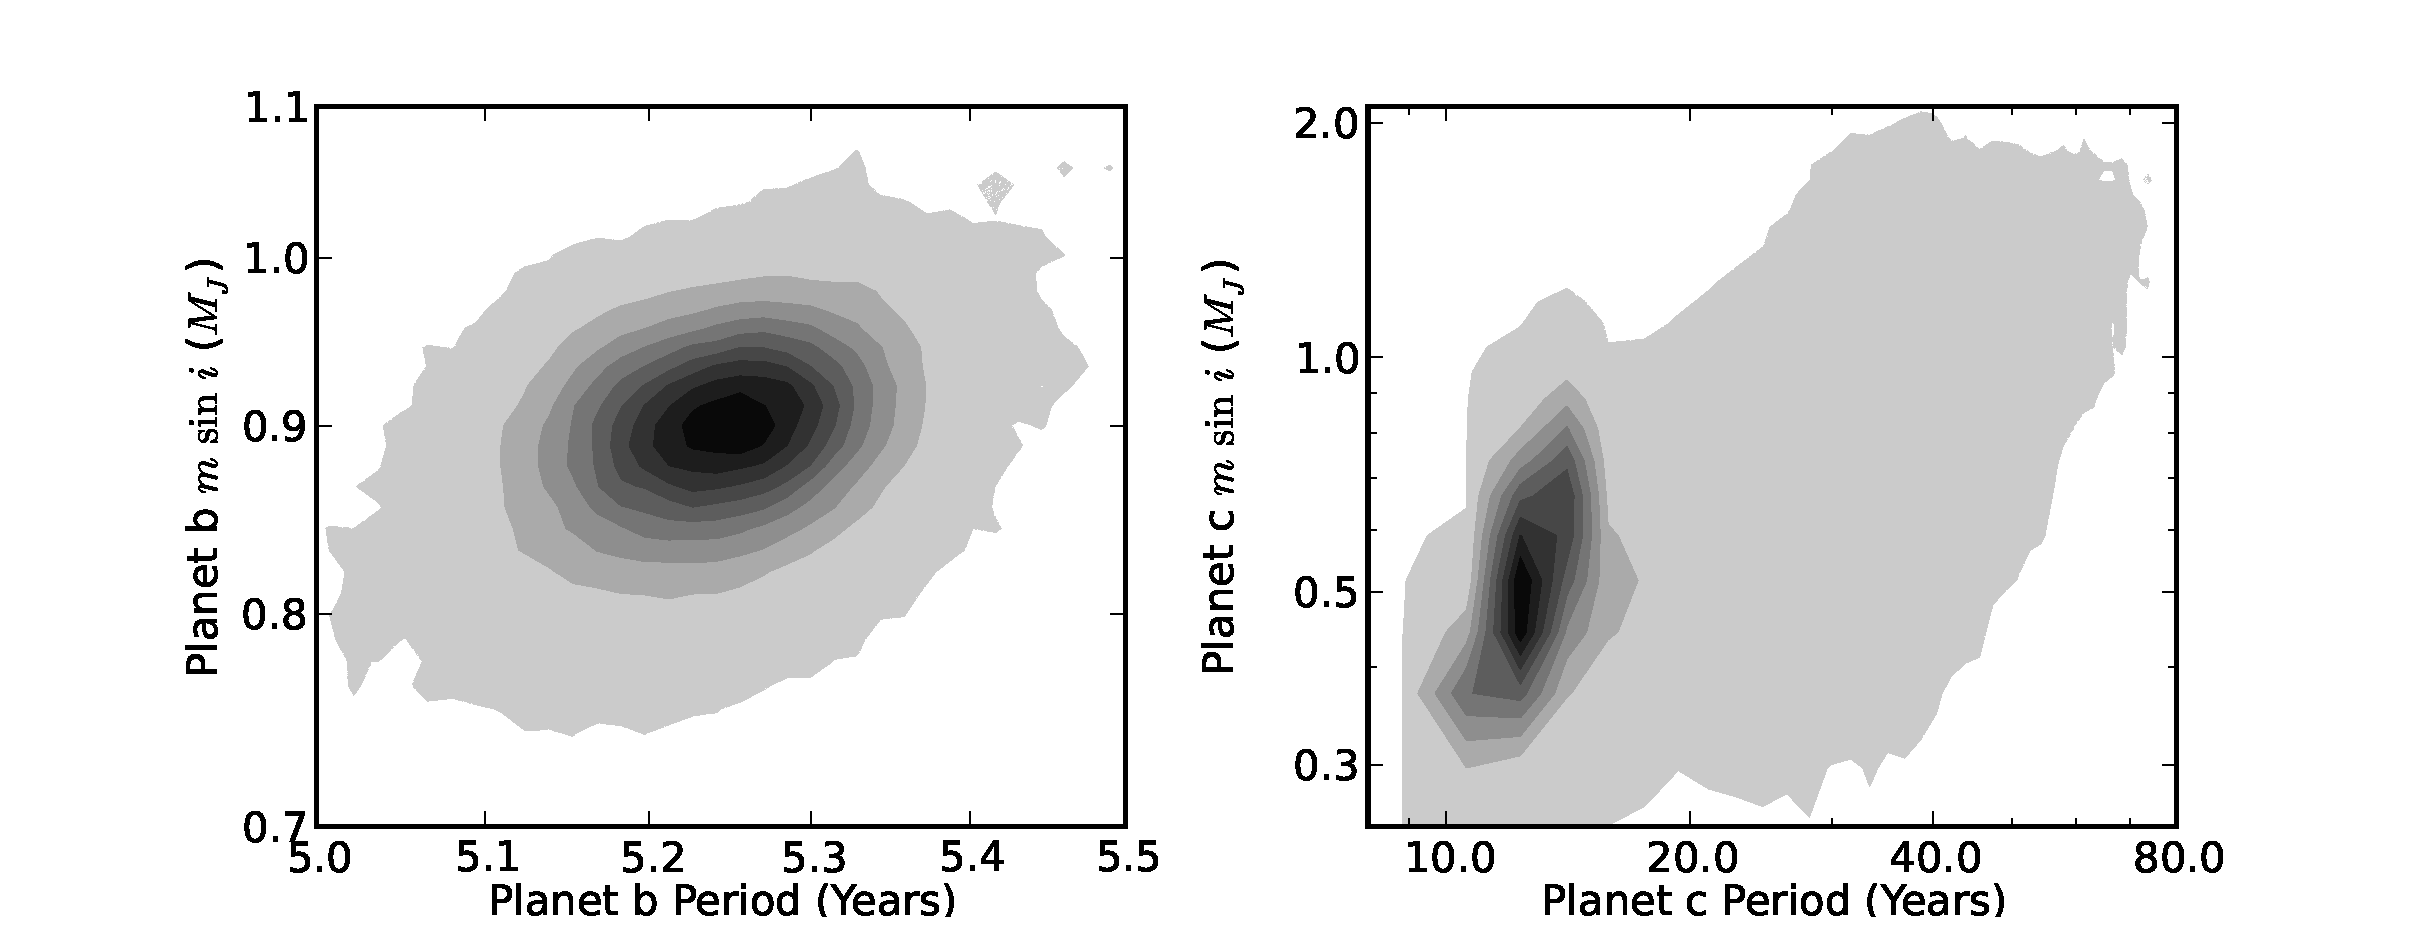
\includegraphics[width=1.0\textwidth]{chapter3/f16.eps}}
\caption[Posterior distributions of allowed masses and periods of 
Gl\,849\,b and Gl\,849\,c]{Position of (left) Gl\,849b and (right) Gl\,849c in the mass-period plane. The orbital parameters for the inner planet are much more tightly constrained than the outer planet. Depending on the exact shape of the planet distribution function, the inner planet may have more than a 50\% probability of being more massive than Jupiter when orientation uncertainties are taken into account.
  }
\label{849}
%\end{landscape}
\end{figure}



\subsection{HIP\,109555}
When observing HIP\,109555 we detected a possible faint companion object located tens of arcseconds away. To prove this companion is not associated with the primary but is instead unrelated, we compare the proper motion of both objects by identifying them in the 2MASS catalog \citep{Skrutskie06} and the Palomar Observatory Sky Survey \citep{Abell59}. Comparing the POSS data collected 16 July 1950 to the 2MASS observation, we detect a proper motion for HIP\,109555 of 0.36 arcsec/yr, consistent with previously published results \citep{vanLeeuwen07}. The hypothetical companion motion, however, is only 5 milliarcseconds per year. Additionally, the companion is bluer in colors derived using the 2MASS J, H, and K filters than HIP\,109555. These are both consistent with the companion being a distant background object, and we neglect its presence in our analysis.

\subsection{HIP\,57050}
\label{HIP57050}
We observed HIP\,57050 (=GJ1148) on December 27, 2012 using the $K_s$ filter on NIRC2. Our imaging is only complete at separations smaller than 1 arcsecond, corresponding to a projected separation of 11 AU. This does not enable us to rule out most stellar companions that could cause our observed RV trends, as shown in Figure \ref{Wright57050}.
\begin{figure}[htbp]
\centerline{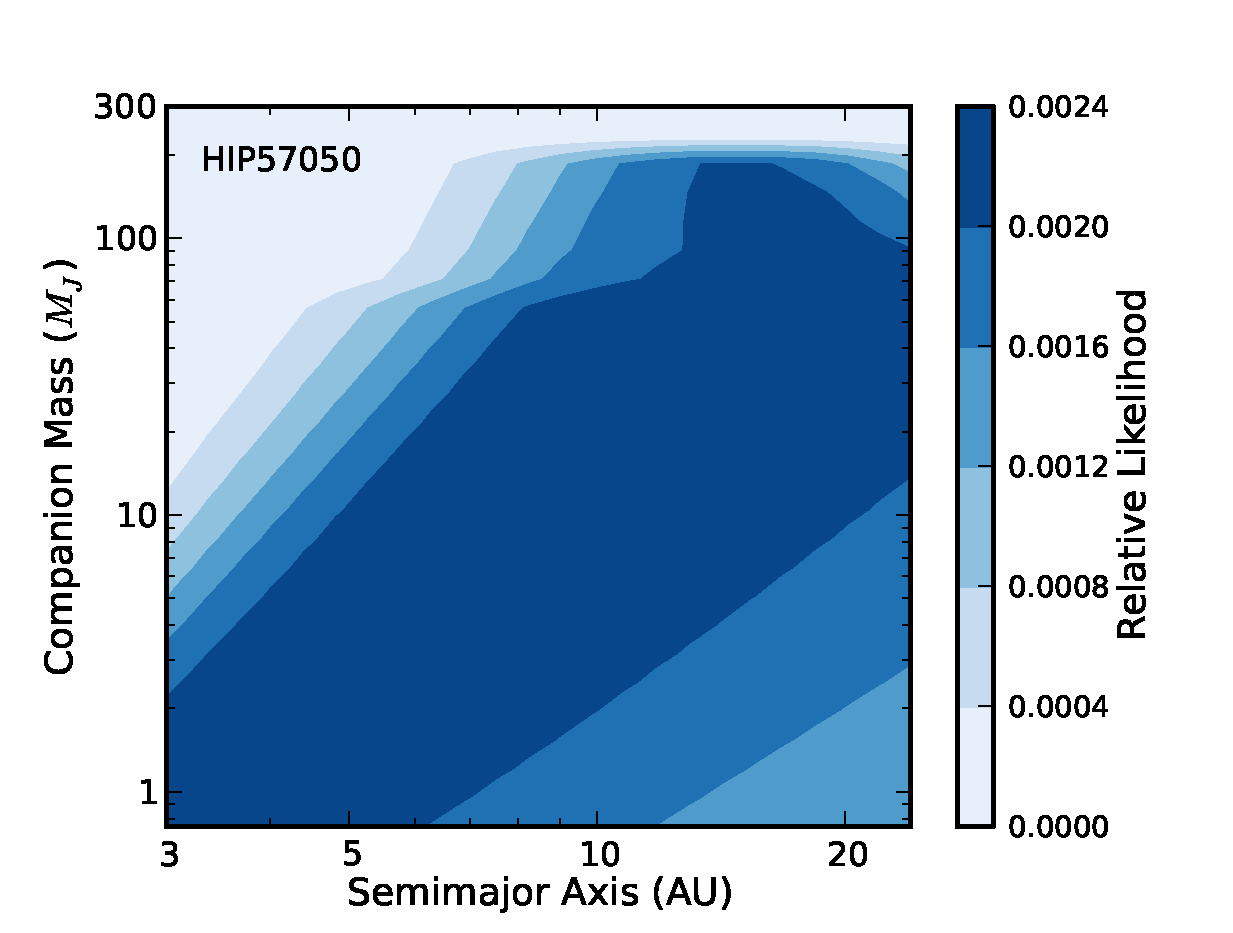
\includegraphics[width=0.75\textwidth]{chapter3/f17.eps}}
\caption[Probability contours displaying the location of a giant companion orbiting HIP\,57050, given that exactly one such planet exists]{Probability contours displaying the location of a giant companion orbiting HIP\,57050, given that exactly one such planet exists, when the RV data is combined with adaptive optics imaging and 2MASS data. Because the AO imagery only extends to 11 AU, there is a small region of parameter space where a low-mass M-dwarf companion could reside. Additional AO observations with a wider field of view would be required to rule out this possibility. Lower-mass companions are allowed in shorter orbital periods due to possible curvature in the radial velocity data.
}
\label{Wright57050}
\end{figure}
If the observed trend is caused by a stellar-mass companion, the companion is likely beyond 10 AU, which corresponds to a separation of 0.9 arcseconds. Thus any stellar companions at their maximum separation that could cause this trend would be expected to be found in a seeing-limited survey. We find no evidence for such a companion. While unlikely, additional AO observations with a wider field of view are required to fully eliminate the possibility that a low-mass star exists. 


\subsection{HIP\,63510}
HIP\,63510B (Ross 458) is an M7 brown dwarf orbiting an M0.5 dwarf at approximately 3 AU \citep{Beuzit04}. Twelve years of RV observations suggest an orbit with a period of 13.9 years, an eccentricity of 0.32, and a minimum mass $m\sin i = 67.9 M_J$, suggesting a nearly edge-on orbit. We estimate a detection efficiency of 1.000 in an RV survey, which is not surprising considering the stellar RV semiamplitude is $K = 1.24$ km s$^{-1}$. This system contains a second companion which is separated from the host star by 1100 AU \citep{Goldman10, Scholz10}

\subsection{HIP\,71898}
HIP\,71898B is an L0 dwarf in a wide orbit around an M3.5 dwarf. \citet{Golimowski04} report a projected separation of $30.01 \pm 3.78$ AU. This target has an RV baseline of 14 years, over which 30 observations were collected. From these observations we measure an acceleration of $8.6 \pm 0.4$ m s$^{-1}$ yr$^{-1}$. At 30 AU, this would suggest a minimum dynamical mass $m \sin i > 45 M_J$, consistent with an L0 dwarf. A detectability plot for companions to HIP\,71898 is shown in Figure \ref{71898}. The observed acceleration lies near a contour representing a 0.9 probability of RV detection, so it is not surprising this companion was detected by CPS. 

\begin{figure}[htbp]
\centerline{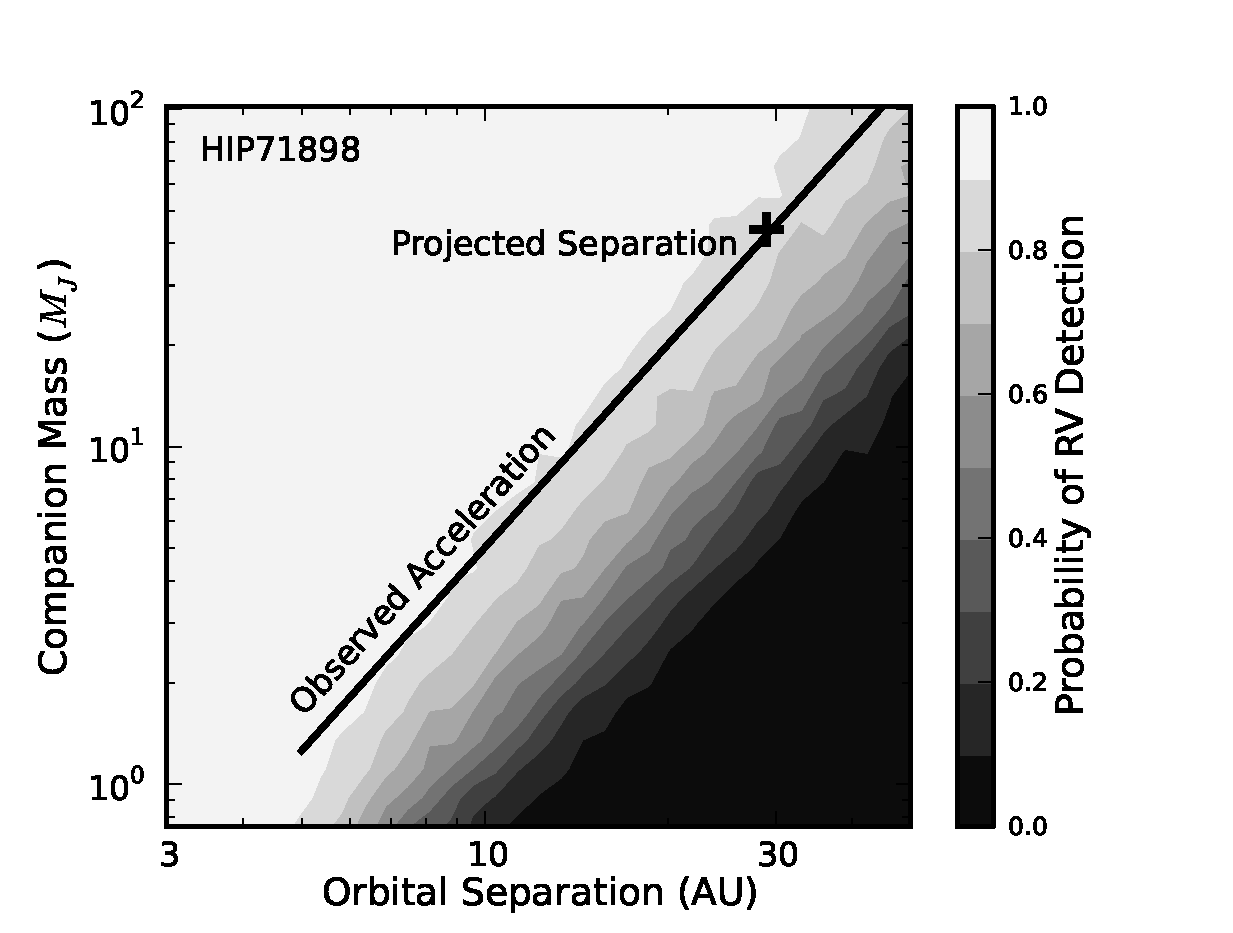
\includegraphics[width=0.75\textwidth]{chapter3/f18.eps}}
\caption[Probability contours displaying the likelihood that a planet of a given mass and semimajor axis would be detected around HIP\,71898 in the CPS RV survey]{ Probability contours displaying the likelihood that a planet of a given mass and semimajor axis would be detected around HIP\,71898 in the CPS RV survey. The diagonal line represents companions that would produce an acceleration of $8.6 \pm 0.4$ m s$^{-1}$ yr$^{-1}$ in an edge on system when the companion was moving along the observer's line of sight. The $+$ marks the spot at which a $45 M_J$ companion at 30 AU would reside; this is the minimum mass and semimajor axis expected from this companion. 
  }
\label{71898}
\end{figure}

\subsection{Gl569}
Gl\,569B is a brown dwarf binary, with an M8.5+M9 pair orbiting each other every $870 \pm 9$ days. The system has a combined mass of $0.140^{+0.009}_{-0.008} M_\odot$ \citep{Dupuy10} and is separated from the primary, an M3.5 dwarf, by a projected separation of 5 arcsec, or 47 AU \citep{Femenia11}. The maximum RV acceleration from such a companion is 3.7 m s$^{-1}$ yr$^{-1}$. For this star, we have a 5.1 year baseline and the median $\sigma$ is 15 m s$^{-1}$. By injecting simulated companions, we estimate an RV detection efficiency near zero for these companions. Thus it is not surprising that it is missed in our sample. 

\subsection{Gl\,229B}
Gl\,229B (HD\,42581) is a T7 dwarf at a projected separation of 44 AU \citep{Faherty09}. This companion has been directly imaged \citep{Nakajima95} but not detected as a strong acceleration through RV variations. As with Gl\,569, this object is beyond our range for efficient brown dwarf detection through RV observations. If we assume a mass of 40 $M_J$, we would expect a maximal RV acceleration of 1.1 m s$^{-1}$ yr$^{-1}$. Thus, again we should not be surprised it is not detected.

\section{A Brief Note on Radial Velocities and Magnetic Activity}
We account for the possibility that any apparent RV accelerations may be induced by magnetic activity statistically, as described in \textsection\ref{FP}. Often, the $S_\textrm{HK}$ value, a measure of the ratio of flux in the Ca II line cores to flux in nearby continuum regions, is taken as a proxy for chromospheric activity \citep{Wilson68, Henry96}. While not a perfect measure, it is comforting to note that the observed radial velocities do not correlate with $S_\textrm{HK}$ in any of our stars with long-term RV accelerations. The RVs for our systems with detected accelerations as well as $S_\textrm{HK}$ for observations after the HIRES detector upgrade are included in Figure \ref{Trendplot} and Table \ref{Txx}. 

\begin{figure}[htbp]
%\begin{landscape}
\centerline{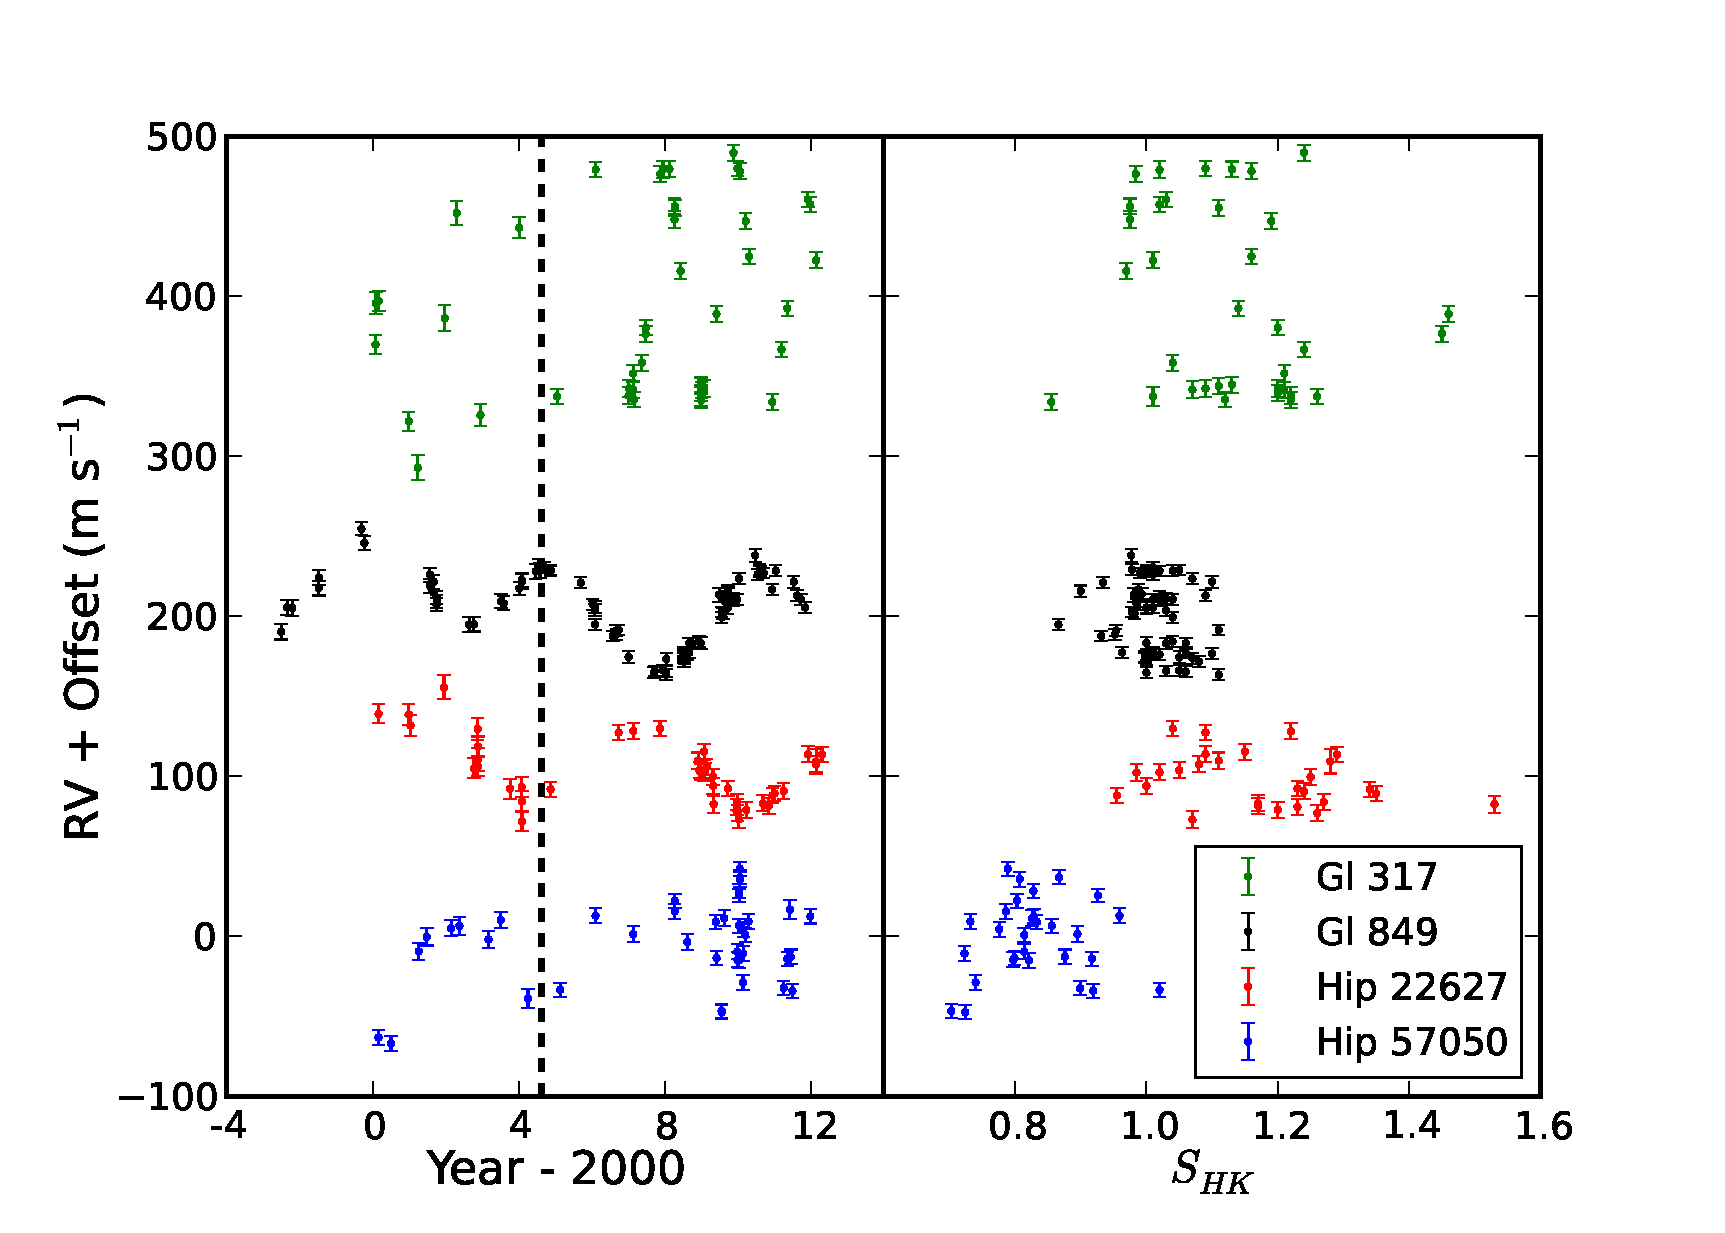
\includegraphics[width=1.0\textwidth]{chapter3/f19.eps}}
\caption[RV time series for our four systems exhibiting long-term RV accelerations and RVs as a function of $S_\textrm{HK}$]{(left) RV time series for our four systems exhibiting long-term RV accelerations. The vertical line in 2004 represents the HIRES detector upgrade in August of that year. (right) RVs as a function of $S_\textrm{HK}$. All four RV accelerations are visible, but none of the RV data appear to correlate with $S_\textrm{HK}$, commonly used as a proxy for stellar chromospheric activity.
  }
\label{Trendplot}
%\end{landscape}
\end{figure}

{\scriptsize
\begin{longtable}{l|ccc||l|ccc} 
\hline
JD-2440000 & RV (m s$^{-1}$) & $\sigma_{\textrm{RV}}$ (m s$^{-1}$) & $S_{\textrm{HK}}$ & JD-2440000 & RV (m s$^{-1}$) & $\sigma_{\textrm{RV}}$ (m s$^{-1}$ & $S_{\textrm{HK}}$ \\
\hline
Gl 317 & & & & & & & \\ 
11550.993 & 369.80 & 5.83 & N/A & 14544.905 & 456.22 & 4.92 & 0.97 \\  
11552.990 & 395.68 & 6.74 & N/A & 14545.894 & 455.37 & 4.96 & 1.11 \\  
11582.891 & 397.16 & 6.08 & N/A & 14603.777 & 415.82 & 5.00 & 0.97 \\  
11883.101 & 321.88 & 5.83 & N/A & 14806.029 & 344.83 & 5.02 & 1.13 \\  
11973.795 & 292.84 & 7.74 & N/A & 14807.069 & 337.39 & 5.70 & 1.01 \\  
12243.073 & 386.34 & 7.95 & N/A & 14808.138 & 343.93 & 4.94 & 1.11 \\  
12362.949 & 451.96 & 7.50 & N/A & 14809.059 & 335.15 & 4.95 & 1.22 \\  
12601.045 & 325.69 & 6.93 & N/A & 14810.161 & 339.65 & 4.87 & 1.20 \\  
12989.125 & 442.81 & 6.64 & N/A & 14811.128 & 341.51 & 4.93 & 1.21 \\  
13369.016 & 337.48 & 4.90 & 1.26 & 14839.107 & 342.36 & 5.26 & 1.09 \\  
13753.983 & 479.22 & 4.85 & 1.13 & 14963.795 & 388.95 & 4.98 & 1.46 \\  
14084.001 & 337.88 & 5.29 & 1.22 & 15134.090 & 489.75 & 4.90 & 1.24 \\  
14086.141 & 342.52 & 5.21 & 1.20 & 15173.079 & 479.92 & 4.79 & 1.09 \\  
14130.082 & 351.80 & 5.37 & 1.21 & 15199.017 & 478.18 & 4.98 & 1.16 \\  
14131.014 & 341.73 & 5.11 & 1.07 & 15255.869 & 447.15 & 4.89 & 1.19 \\  
14138.932 & 335.57 & 4.86 & 1.12 & 15289.857 & 424.86 & 4.82 & 1.16 \\  
14216.733 & 358.57 & 4.95 & 1.04 & 15522.057 & 333.93 & 4.97 & 0.85 \\  
14255.743 & 376.54 & 4.92 & 1.45 & 15613.960 & 366.70 & 4.92 & 1.24 \\  
14255.749 & 380.38 & 4.79 & 1.20 & 15672.848 & 392.45 & 4.92 & 1.14 \\  
14400.110 & 476.46 & 4.91 & 0.98 & 15878.127 & 460.49 & 4.81 & 1.03 \\  
14428.062 & 479.05 & 5.29 & 1.02 & 15903.017 & 457.41 & 4.79 & 1.02 \\  
14492.901 & 479.46 & 5.05 & 1.13 & 15960.986 & 422.57 & 4.98 & 1.01 \\  
14543.948 & 448.01 & 5.34 & 0.97 &  &  &  &  \\  
\hline
Gl 849 & & & & & & & \\ 
10606.068 & 190.31 & 4.78 & N/A & 14455.744 & 165.29 & 3.45 & 1.06 \\  
10666.001 & 205.60 & 4.69 & N/A & 14456.733 & 163.51 & 3.48 & 1.11 \\  
10715.957 & 205.19 & 4.99 & N/A & 14460.742 & 173.41 & 3.53 & 1.00 \\  
10983.038 & 217.69 & 4.67 & N/A & 14634.083 & 176.64 & 3.34 & 1.10 \\  
10984.084 & 224.23 & 4.55 & N/A & 14635.042 & 173.89 & 3.32 & 1.00 \\  
11410.021 & 254.67 & 4.08 & N/A & 14636.051 & 176.71 & 3.33 & 1.01 \\  
11439.865 & 245.85 & 4.30 & N/A & 14637.116 & 176.23 & 3.31 & 1.00 \\  
12095.081 & 225.97 & 4.52 & N/A & 14638.059 & 177.42 & 3.41 & 0.96 \\  
12096.046 & 219.06 & 4.38 & N/A & 14639.067 & 174.78 & 3.42 & 1.00 \\  
12133.013 & 221.49 & 4.39 & N/A & 14640.115 & 171.70 & 3.36 & 1.08 \\  
12160.909 & 211.60 & 4.10 & N/A & 14641.117 & 173.84 & 3.38 & 1.07 \\  
12161.846 & 207.39 & 4.19 & N/A & 14644.113 & 177.39 & 3.40 & 1.01 \\  
12162.887 & 209.34 & 4.22 & N/A & 14674.936 & 176.17 & 3.40 & 1.02 \\  
12486.968 & 194.80 & 4.66 & N/A & 14688.952 & 177.11 & 3.40 & 1.06 \\  
12535.852 & 194.96 & 4.43 & N/A & 14690.005 & 183.22 & 3.51 & 1.06 \\  
12807.011 & 209.44 & 4.30 & N/A & 14721.949 & 183.11 & 3.52 & 1.03 \\  
12834.013 & 208.07 & 4.39 & N/A & 14790.752 & 184.27 & 3.43 & 1.04 \\  
12989.720 & 217.41 & 4.08 & N/A & 14807.793 & 183.33 & 3.47 & 1.00 \\  
13014.710 & 222.75 & 4.27 & N/A & 14989.063 & 213.37 & 4.17 & 0.98 \\  
13015.711 & 221.97 & 4.60 & N/A & 15015.047 & 199.35 & 3.42 & 1.04 \\  
13016.706 & 222.33 & 4.07 & N/A & 15016.074 & 202.71 & 3.36 & 0.98 \\  
13154.080 & 228.16 & 4.76 & N/A & 15029.019 & 201.72 & 3.52 & 0.98 \\  
13180.108 & 231.43 & 4.45 & N/A & 15043.042 & 212.32 & 3.40 & 1.02 \\  
13196.931 & 228.82 & 4.63 & N/A & 15048.996 & 209.45 & 3.39 & 0.98 \\  
13238.929 & 230.55 & 3.44 & 1.01 & 15075.082 & 205.14 & 3.55 & 1.00 \\  
13301.838 & 228.44 & 3.39 & 1.00 & 15080.084 & 215.78 & 3.50 & 0.90 \\  
13302.742 & 228.98 & 3.32 & 1.05 & 15082.073 & 213.97 & 3.44 & 0.99 \\  
13303.798 & 228.40 & 3.27 & 1.02 & 15134.922 & 210.04 & 3.41 & 1.02 \\  
13603.939 & 221.04 & 3.43 & 0.93 & 15135.876 & 210.90 & 3.37 & 1.03 \\  
13724.712 & 207.52 & 3.39 & 0.98 & 15169.797 & 210.64 & 3.55 & 1.01 \\  
13746.715 & 205.70 & 3.60 & 1.01 & 15188.725 & 223.58 & 3.42 & 1.07 \\  
13746.721 & 203.74 & 3.72 & 1.03 & 15352.082 & 238.03 & 4.18 & 0.98 \\  
13749.698 & 194.88 & 3.51 & 0.87 & 15376.032 & 226.26 & 3.36 & 1.01 \\  
13927.015 & 187.71 & 3.42 & 0.93 & 15395.958 & 229.16 & 3.32 & 0.98 \\  
13959.087 & 191.03 & 3.34 & 1.90 & 15397.048 & 227.85 & 3.36 & 1.00 \\  
13960.955 & 188.72 & 3.31 & 0.95 & 15436.111 & 227.10 & 3.40 & 0.99 \\  
13960.962 & 191.05 & 3.32 & 0.95 & 15521.801 & 216.77 & 3.53 & 0.99 \\  
13983.000 & 191.46 & 3.36 & 1.11 & 15555.792 & 228.55 & 3.38 & 1.04 \\  
14083.750 & 174.45 & 3.67 & 1.05 & 15736.122 & 221.64 & 3.86 & 1.10 \\  
14337.074 & 164.82 & 3.45 & 1.00 & 15770.878 & 212.94 & 3.41 & 1.09 \\  
14343.872 & 165.90 & 3.35 & 1.03 & 15807.063 & 210.62 & 3.40 & 1.04 \\  
14429.742 & 166.12 & 3.44 & 1.05 & 15851.759 & 205.57 & 3.33 & 1.00 \\  
\hline
Hip 22627 & & & & & & & \\ 
11580.831 & 139.11 & 6.00 & N/A & 14838.995 & 115.36 & 5.10 & 1.15 \\  
11882.888 & 138.64 & 6.58 & N/A & 14846.957 & 102.80 & 5.28 & 2.81 \\  
11901.002 & 131.80 & 6.77 & N/A & 14864.957 & 105.69 & 5.05 & 1.97 \\  
12235.849 & 155.64 & 7.57 & N/A & 14928.732 & 99.68 & 4.86 & 1.25 \\  
12536.088 & 105.11 & 6.31 & N/A & 14929.726 & 94.02 & 5.14 & 1.00 \\  
12572.991 & 129.52 & 6.78 & N/A & 14934.731 & 82.53 & 5.28 & 1.53 \\  
12573.950 & 118.58 & 6.32 & N/A & 15077.110 & 92.45 & 4.91 & 1.23 \\  
12575.047 & 106.25 & 6.29 & N/A & 15170.784 & 80.88 & 5.08 & 1.23 \\  
12575.991 & 110.57 & 7.00 & N/A & 15170.791 & 84.01 & 5.07 & 1.27 \\  
12898.116 & 92.25 & 6.13 & N/A & 15174.093 & 77.01 & 5.12 & 1.26 \\  
13014.818 & 93.28 & 6.34 & N/A & 15187.837 & 72.99 & 5.07 & 1.07 \\  
13015.832 & 84.39 & 6.15 & N/A & 15261.771 & 79.05 & 5.15 & 1.20 \\  
13016.832 & 71.79 & 5.78 & N/A & 15429.120 & 83.25 & 5.07 & 1.17 \\  
13302.975 & 91.91 & 4.79 & 1.34 & 15487.096 & 81.47 & 4.81 & 1.17 \\  
13984.089 & 127.34 & 4.92 & 1.09 & 15522.938 & 88.05 & 4.89 & 0.95 \\  
14130.853 & 128.24 & 5.10 & 1.22 & 15545.819 & 89.25 & 4.89 & 1.35 \\  
14397.938 & 129.88 & 4.87 & 1.04 & 15636.775 & 90.74 & 4.87 & 1.24 \\  
14778.991 & 109.83 & 5.06 & 1.11 & 15879.984 & 113.81 & 4.90 & 1.09 \\  
14790.995 & 103.81 & 5.07 & 1.05 & 15960.761 & 109.29 & 7.51 & 1.28 \\  
14807.917 & 102.51 & 4.97 & 1.02 & 15960.765 & 107.53 & 4.93 & 1.08 \\  
14838.988 & 102.33 & 5.11 & 0.98 & 16019.733 & 113.58 & 4.78 & 1.29 \\  
\hline
Hip 57050 & & & & & & & \\ 
11581.046 & -63.25 & 4.53 & N/A & 15172.138 & -9.58 & 4.64 & 0.81 \\  
11705.827 & -67.09 & 4.79 & N/A & 15174.138 & -14.72 & 4.67 & 0.80 \\  
11983.009 & -9.42 & 5.27 & N/A & 15188.151 & -14.99 & 4.64 & 0.82 \\  
12064.864 & -0.39 & 5.34 & N/A & 15189.155 & 6.60 & 4.25 & 0.86 \\  
12308.077 & 4.98 & 5.01 & N/A & 15190.153 & 25.56 & 4.11 & 0.93 \\  
12391.034 & 6.53 & 5.63 & N/A & 15191.133 & 28.40 & 4.36 & 0.83 \\  
12681.050 & -1.92 & 5.15 & N/A & 15197.136 & 42.23 & 4.28 & 0.79 \\  
12804.885 & 10.26 & 5.05 & N/A & 15198.054 & 35.70 & 4.59 & 0.81 \\  
13077.104 & -38.83 & 5.83 & N/A & 15199.170 & 36.95 & 4.42 & 0.87 \\  
13398.975 & -33.44 & 4.33 & 1.02 & 15229.114 & -28.84 & 4.45 & 0.74 \\  
13753.068 & 12.88 & 4.64 & 0.96 & 15229.958 & -10.72 & 4.71 & 0.72 \\  
14131.092 & 1.32 & 4.96 & 0.90 & 15232.054 & 4.35 & 4.63 & 0.78 \\  
14545.002 & 15.61 & 4.55 & 0.79 & 15251.997 & 0.76 & 4.38 & 0.81 \\  
14546.007 & 22.29 & 4.29 & 0.80 & 15284.858 & 9.29 & 4.64 & 0.73 \\  
14671.811 & -3.54 & 5.13 & 5.32 & 15636.023 & -32.36 & 4.31 & 0.90 \\  
14955.894 & 9.12 & 4.47 & 0.83 & 15671.915 & -13.93 & 4.34 & 0.92 \\  
14963.930 & -13.66 & 4.43 & 0.80 & 15698.820 & 16.56 & 5.97 & 7.95 \\  
15014.782 & -46.65 & 4.50 & 0.70 & 15707.812 & -12.89 & 4.66 & 0.88 \\  
15015.804 & -47.40 & 4.41 & 0.72 & 15723.769 & -34.04 & 4.41 & 0.92 \\  
15041.758 & 11.31 & 5.04 & 0.83 & 15903.064 & 12.42 & 4.40 & 0.83  \\
\hline
\caption{RVs and $S_{\textrm{HK}}$ values for systems with long-term RV accelerations}
\label{Txx}
\end{longtable}
}






\chapter{Physical Properties of the Transiting Brown Dwarf LHS\,6343\,C}
\label{chap:lhs1}


In this chapter I focus on LHS\,6343\,C, a brown dwarf transiting one member of an M+M binary in the \kep\ field.
Given the relative brightness of the host star and the high signal-to-noise ratio on the individual transits themselves,
analyzing this system was a test of the limits of \kep\ data: given a sufficiently high signal transit, what limits our precision?
Are there any assumptions we often make, such as details of limb darkening, that will eventually break down? 
Are there any robust methods to characterize the star without relying on the fine details of any particular set of stellar models?
This chapter was originally published as ``Characterizing the Cool KOIs. VII. Refined Physical Properties of the Transiting Brown Dwarf LHS\,6343\,C,'' ApJ, 800, 134 (2015) by BTM, John Johnson, Phil Moorhead, Ashley Villar, Corinne Vassallo,
Cristoph Baranec, Nick Law, Reed Riddle, Geoff Marcy, Andrew Howard, and Howard Isaacson.


\section{Introduction}
\label{sec:intro-4}

The growth of brown dwarf astronomy has closely mirrored that of exoplanetary astronomy.
Although \citet{Latham89} discovered a likely brown dwarf candidate, the first confirmed detection of a brown dwarf was announced two months before the announcement of the first exoplanet orbiting a main sequence star \citep{Mayor95, Rebolo95}. 
That same year also saw the discovery of the first brown dwarf orbiting a stellar-mass companion \citep{Nakajima95}. 
Today, more than 2,000 brown dwarfs have been discovered.
The majority of these substellar objects have no detected companions, so characterization is often limited to spectroscopic observations.
In these cases, the atmosphere of the brown dwarf can be extensively studied \citep[e.g.][]{Burgasser14, Faherty14}, but its physical parameters, including mass and radius, cannot be measured directly.

When a brown dwarf with a gravitationally bound companion is detected, detailed characterization of its physical properties is possible. 
Radial velocity (RV) surveys have produced a significant number of brown dwarf candidates with minimum mass determinations \citep[e.g.][]{Patel07}. 
Astrometric monitoring of directly imaged brown dwarf companions to stars has led to dynamical mass measurements of brown dwarfs \citep{Liu02, Dupuy09, Crepp12a}.
While there are many brown dwarfs with measured masses, radii can only be directly measured in transiting or eclipsing systems.
The first eclipsing brown dwarf system, discovered by \citet{Stassun06} in the Orion Nebula, produced the first measurement of a brown dwarf's radius and the first test of theoretical mass-radius relations.
Today, there are eleven brown dwarfs with measured masses and radii \citep{Diaz14b}. 
Of this sample, eight transit a stellar-mass companion and only four are not inflated due to youth or irradiation.
If the brown dwarf is assumed to be coeval with its host star, the brown dwarf's age and metallicity can be estimated. Both properties are expected to affect the brown dwarf mass-radius relation, making observations of transiting brown dwarfs especially valuable \citep{Burrows11}. 

Recently, four brown dwarfs have been detected by the \itk{} mission \citep{Bouchy11b, Johnson11a, Diaz13, Moutou13}.
Launched in 2009, the \itk{} telescope collected wide-field photometric observations of approximately 200,000 stars in Cygnus and Lyra every 30 minutes for 4 years \citep{Borucki10}. 
The mission was designed as a search for transiting planets.
As brown dwarfs have radii similar to Jupiter, brown dwarfs were also easily detected; only a few RV observations are necessary to distinguish between a giant planet and brown dwarf companion \citep[e.g.][]{Moutou13}.

The first unambiguous brown dwarf detected from \itk{} data was found in the \LHS{} system and announced by \citet[hereafter J11]{Johnson11a}. 
The authors analyzed five transits of the primary star observed in the first six weeks of \itk{} data, combined with one transit observed in the Z-band with the Nickel telescope at Lick observatory and 14 RV observations with Keck/HIRES.  
The authors also obtained PHARO adaptive optics imaging data from the Palomar 200 inch telescope, imaging a companion 0.5 magnitudes fainter than the primary at a separation of 0.7 arcsec. 
From these observations, the authors were able to measure a mass for the brown dwarf of $62.7 \pm 2.4$ \mjup{}, a radius of $0.833 \pm 0.021$ \rjup, and a period of $12.71$ days, corresponding to a semimajor axis of $0.0804\pm0.0006$ AU.
The authors define \LA{} as the primary star, \LB{} as the widely-separated binary M dwarf, and \LC{} as the brown dwarf orbiting the A component, and note the architecture of this system is very similar to the NLTT\,41135 system discovered by \citet{Irwin10}.

Additional papers have expanded our knowledge of \LHS. 
\citet{Southworth11} re-fit the \itk{} light curve, using data through Quarter 2 from the mission. By fitting the observations using five different sets of stellar models, he attempted to reduce biases caused by any one individual stellar model. He found different models provide a consistent brown dwarf radius at the $0.08$ \rjup{} level, but found a higher mass than J11: his best fitting mass for \LC{} was $70 \pm 6$ \mjup.
\citet{Oshagh12} analyzed the lack of transit timing variations in the system, finding that any additional companions to \LA{} with an orbital period smaller than 100 days must have a mass smaller than that of Jupiter. 
With 6 quarters of \itk{} data, \citet{Herrero13} measured a photometric rotation period of $13.13 \pm 0.02$ days for \LA. 
The authors also claimed to observe spot-crossing events during the transits of \LA{}, as well as out-of-transit photometric modulation with a period consistent with the orbital period of \LC. 
\citet{Herrero14} updated this work, concluding that the out-of-transit variations are dominated by relativistic Doppler beaming.

In many of the papers about the \LHS{} system after the discovery paper, the authors assumed the physical parameters of J11. 
This is not necessarily an ideal assumption to make.
J11 used a limited dataset during their analysis.
Their photometry consisted of only six transits and 14 RVs, and they estimated the third light contribution of \LB{} by extrapolating from near-IR observations to the \itk{} bandpass.
Moreover, the derived stellar parameters in that paper were based only on photometric observations and depend strongly on the accuracy of the Padova model grids \citep{Girardi02} upon which they are based.

The conclusion of the primary \itk{} mission affords us an opportunity to reanalyze the \LHS{} system using the complete \itk{} dataset. 
Such a reanalysis enables us to better measure the brown dwarf's mass and radius. 
There are only three non-inflated brown dwarfs with both a mass and radius measured to $5\%$ or better: \LC, KOI-205 b \citep{Diaz13}, and KOI-415 b \citep{Moutou13}.  
To test theoretical brown dwarf evolutionary models, we would like to measure the masses, radii, and metallicities of these objects as precisely as possible. 
In this work, we analyze the full \itk{} dataset for this object to measure the transit profile.
We combine this light curve with additional RV observations, near-infrared spectroscopy of \LA B, and Robo-AO visible-light adaptive optics.
Without any reliance on stellar models beyond an empirical main sequence mass-radius relation, we are able to measure the mass of \LC{} to a precision of 3\% and the radius to a precision of 2\%. 
Beyond the empirical main-sequence relation, the mass and radius measurements depend only on the following parameters, all measured directly from the data: the orbital period, stellar density \rhostar, reduced semimajor axis $a/$\rstar, Doppler semiamplitude $K$, eccentricity, and inclination.
Our technique allows one to calculate the mass and radius for both members of a transiting system.
We also combine our data with the predictions for the mass of \LA{} from the Dartmouth stellar evolutionary models of \citet{Dotter08}.
These combined data enable us to measure a model-dependent mass and radius of \LC{} to better than $2\%$ each; we also measure a metallicity of the system of $0.02 \pm 0.19$ dex. 

In Section 4.2 we describe the observations used in this paper. 
In Section 4.3 we outline our data analysis pipeline. 
In Section 4.4 we present our results.
In Section 4.5 we summarize our present efforts and outline our future plans to measure the brown dwarf's luminosity.


This study presents, to date, the most precise mass and radius measurements of a non-inflated brown dwarf. 
Observations such as these are essential for future detailed characterization of field brown dwarfs.



\section{Observations}
\subsection{\itk\ Photometry}

The \LHS{} system (KIC 10002261, KOI-959) was part of the initial \itk{} target selection and was observed during all observing quarters in long cadence mode.
Between 22 February 2011 and 14 March 2011, the system was also observed using \itk's short cadence mode, with observations collected every 58.84876 seconds in the reference frame of the spacecraft. 
We downloaded the entire dataset from the NASA Multimission Archive at STScI (MAST). 

For both long and short cadence observations, \itk{} data consist of a postage stamp containing tens of pixels, a small number of which are combined to form an effective aperture.
The flux from all pixels in the aperture are combined to create a light curve. 
The \itk{} team defines an aperture for all targets and performs aperture photometry as a part of their Photometric Analysis (PA) pipeline, which produces a light curve from the pixel-level data \citep{Jenkins10}. 
This pipeline also removes the photometric background and cosmic rays. 

In analyzing the pipeline-generated light curve, we detected occasional anomalies during transit events, with the recorded flux systematically larger than expected.
These anomalies were also detected by \citet{Herrero13}, who attribute them to occultations of spots on \LA{} by \LC. 
The anomalies occur only in the long cadence data, and only when the transit is symmetric around one data point in the \itk{} time series, so that the central in-transit flux measurement would be expected to be significantly lower than the surrounding data points.
By investigating the pixel-level data, we find that each anomaly has been registered as a cosmic ray by the PA pipeline, and ``corrected'' to an artificially large value.

Using the pixel-level data, recorded before the cosmic ray correction in the pipeline, we removed these artificial corrections. 
We find the anomalies can be completely explained as false cosmic ray detections: there is no evidence for transit-to-transit variability in the \itk{} data.

We expect stellar granulation to induce correlated photometric variability only at a level significantly below the precision of our observations.
Correlated noise attributed to stellar granulation has been previously observed when modeling transits of companions to higher mass stars \citep[e.g.][]{Huber13} and used to derive fundamental parameters of the stars themselves \citep{Bastien13}.
Both the timescale and magnitude of the correlated noise are inversely proportional to the stellar density \citep{Gilliland10}.
For an M dwarf with a mass around 0.3\msun, we expect granulation to induce correlated noise with a period of approximately 10 seconds and an amplitude of 50 ppm \citep{Winget91}. 
Therefore, given the precision and cadence of the \itk{} observations we do not expect to observe correlated noise due to granulation in the \LHS{} system. 

We tested for correlated noise on transit timescales by calculating the autocorrelation matrix for out-of-transit sections of the data. For both long cadence and short cadence data, all off-diagonal elements have absolute values less than 0.03; we found no periodic structure to the autocorrelation matrix. 
Therefore, on transit timescales the noise can be treated as white.

We converted all times recorded by \itk{} to Barycentric Dynamical Time (TDB), not UTC, which was mistakenly recorded during the first three years of the mission. 
As a result, our times differ from those reported in the analysis of J11 by 66.184 seconds.

We then detrended the light curve to remove the effects of stellar and instrumental variability. 
For all transit events with at least four data points recorded continuously before and after the transit, we selected a region bounded by a maximum of three transit durations on either side of the nominal transit center.
If there is any spacecraft motion, such as a thruster fire or data downlink, we clipped the fitting region to not include these data.
We then fit a second-order polynomial to the out of transit flux. 
We normalized the light curve by dividing the observed flux values by the calculated polynomial. 
We repeated this procedure near the midpoint between successive transits in order to search for evidence of a secondary eclipse. 
We estimated the noise level in the data by measuring the variance observed in the out of transit segments of the data.

\subsection{Keck/HIRES Radial Velocities}

We obtained spectroscopic observations of \LHS{} using the HIgh Resolution Echelle Spectrometer (HIRES, $R \approx 48$,000) at the W. M. Keck Observatory. 
All observations were taken using the C2 decker. 
With a projected length of 14.0 arcsec, the decker enables accurate sky subtraction. 
The first four observations were obtained using a 45 minute exposure time and the standard iodine-cell setup described by \citet{Howard10}. 
Once \LC{} was identified as an transiting brown dwarf, the remaining observations were obtained with 3 minute exposure times and without the iodine cell.
For all observations, the slit was aligned along the binary axis so that light from both stars fell upon the detector. 

To measure the RV of \LA, we used \LB{} as a wavelength reference. 
We began with an iodine-free spectrum of HIP 428, oversampled onto a grid with resolution 15 m s$^{-1}$.
For each observation, we restricted our analysis to the 16 orders covered by the ``green'' CCD chip, which covers the region typically used in iodine cell analyses, as well as the first two orders covered by the ``red'' chip where telluric contamination is negligible.
From these 18 orders, we first estimated and divided out the continuum flux level following the method of \citet{Pineda13}. 
We then removed the regions of the spectrum contaminated by telluric lines.
We added to this template a shifted, scaled version of itself to represent \LB.
We varied the positions of both stars and compared to the observed spectrum of \LHS{} in order to find the maximum likelihood velocity separation between the two stars.
By assuming the relative RV of \LB{} does not change over our observing baseline, our method enables us to measure the RV of \LA{} relative to that of a stationary wavelength calibration source observed simultaneously. 

There is no evidence of orbital motion of \LB{} at the level of our RV precision.
From an observed projected separation and mass estimate we can estimate the maximum expected RV acceleration induced by a companion.
Following \citet{Torres99} and \citet{Knutson14}, the maximum RV acceleration is defined such that 
\begin{equation}
\left|{\dot{v}}\right| < 68.8 {\textrm m\phantom{0}s^{-1}\phantom{0}yr^{-1}} \bigg( \frac{M_{\textrm comp}}{M_{\textrm Jup}}\bigg) \left(\frac{d}{\textrm pc}\frac{\rho}{\textrm arcsec}\right)^{-2},
\end{equation}
for a system at a distance $d$, with a companion with mass $M_\textrm{comp}$ at an angular separation $\rho$.
For a companion with a mass approximately 30\% of the Sun's and a projected separation ($d\rho$) of approximately 20 AU, we expect a maximum RV acceleration of 40 m s$^{-1}$ yr$^{-1}$.
We would only observe this RV acceleration if we happened to observe the two stars at the time of their maximum orbital separation and if their orbit was edge-on to our line of sight. 
Our RV signal is considerably larger than any effects induced by \LB; any RV acceleration over our three-year baseline is similar in size to our measurement uncertainties.

The median RV precision of our observations is 85 m s$^{-1}$.
Our RV precision is much lower ($\approx 400$ m s$^{-1}$) for the first four observations when the spectra are contaminated by the iodine cell. 
Our RV precision is also impeded when the difference between the RV of \LA{} and \LB{} is smaller than one-half of a pixel, about 500 m s$^{-1}$.

A table of our RVs is included as Table \ref{RVTable}.

\begin{table}[hbt!]
\centering
\begin{tabular}{lcc}
\hline
JD $- 2440000$ & RV (km s$^{-1}$) & Uncertainty (km s$^{-1}$) \\
\hline
15373.095 & 12.993 & 0.498 \\ 
15373.998 & 13.878 & 0.429 \\ 
15377.078 & 3.041 & 0.425 \\ 
15377.098 & 2.825 & 0.423 \\ 
15378.030 & -2.470 & 0.562 \\ 
15379.052 & -4.599 & 0.076 \\ 
15380.127 & -5.967 & 0.082 \\ 
15380.827 & -5.412 & 0.089 \\ 
15380.831 & -5.015 & 0.166 \\ 
15395.984 & 3.726 & 0.084 \\ 
15396.970 & 8.522 & 0.068 \\ 
15404.974 & -5.447 & 0.092 \\ 
15405.821 & -5.618 & 0.074 \\ 
15406.865 & -3.860 & 0.086 \\ 
15407.853 & -0.495 & 0.666 \\ 
15413.032 & 11.540 & 0.072 \\ 
15414.009 & 7.951 & 0.089 \\ 
15668.120 & 8.714 & 0.161 \\ 
15669.083 & 4.243 & 0.174 \\ 
15673.982 & -3.661 & 0.083 \\ 
15705.917 & 10.005 & 0.093 \\ 
15843.859 & 13.444 & 0.084 \\ 
16116.017 & -3.562 & 0.077 \\ 
16164.014 & 8.408 & 0.064 \\ 
16172.915 & 10.070 & 0.078 \\ 
16192.886 & -4.885 & 0.073 \\ 
16498.042 & -5.035 & 0.079 \\ 
16506.891 & 9.963 & 0.073 \\ 
16513.001 & -3.995 & 0.081 \\ 
16513.988 & 0.033 & 0.733 \\ 
16522.939 & -3.889 & 0.078 \\ 
16524.890 & -5.555 & 0.113 \\ 
16524.892 & -5.473 & 0.081 \\ 
16530.943 & 13.348 & 0.092  \\
\hline
\end{tabular}
\caption{Radial Velocities for LHS\,6343\,A}
\label{RVTable}
\end{table}



\subsection{Visible-light Adaptive Optics Imaging}

J11 estimated the third-light contribution of \LB{} in the \itk{} bandpass by extrapolating from JHK adaptive optics observations using the Padova model atmospheres of \citet{Girardi02}. 
To minimize any potential biases that may be induced by their reliance on stellar models, we obtained adaptive optics imaging of \LHS{} with the Robo-AO laster adaptive optics and imaging system on the Palomar Observatory 60-inch telescope \citep{Baranec14}. 
Robo-AO successfully observed thousands of KOIs; we used their standard setup \citep{Law14}. 
With SDSS $g$, $r$, and $i$ filters \citep{York00}, we imaged the system on UT 2013 21 July; we observed the system again in $g$ band on UT 2013 27 July. 
Each observation consisted of full-frame-detector readouts at 8.6 Hz for 90 seconds. 
We use 100\% of the frames during each integration.
The images were then combined using a shift-and-add processing scheme, using \LA{} as the tip-tilt star. 
At all wavelengths, we detected both \LA{} and \LB, as shown in Figure \ref{AOPlot}.
While we would be sensitive to a change in the position angle between the two M dwarfs of two degrees, we do not detect any orbital motion of \LB{} relative to \LA{} between the original Palomar/PHARO data in 2010 and these observations in 2013.


To calculate the relative flux ratio of the two stars in each bandpass, we sky-subtract our observations and measure the flux inside a 0.5 arcsec aperture centered on each star. 
The point spread functions of each star are larger than the apertures, so each aperture contains light from both stars. We subtract out the contamination from each star by measuring the flux in a similar aperture on the opposite side of each star. 


\begin{figure}[htbp!]
\centerline{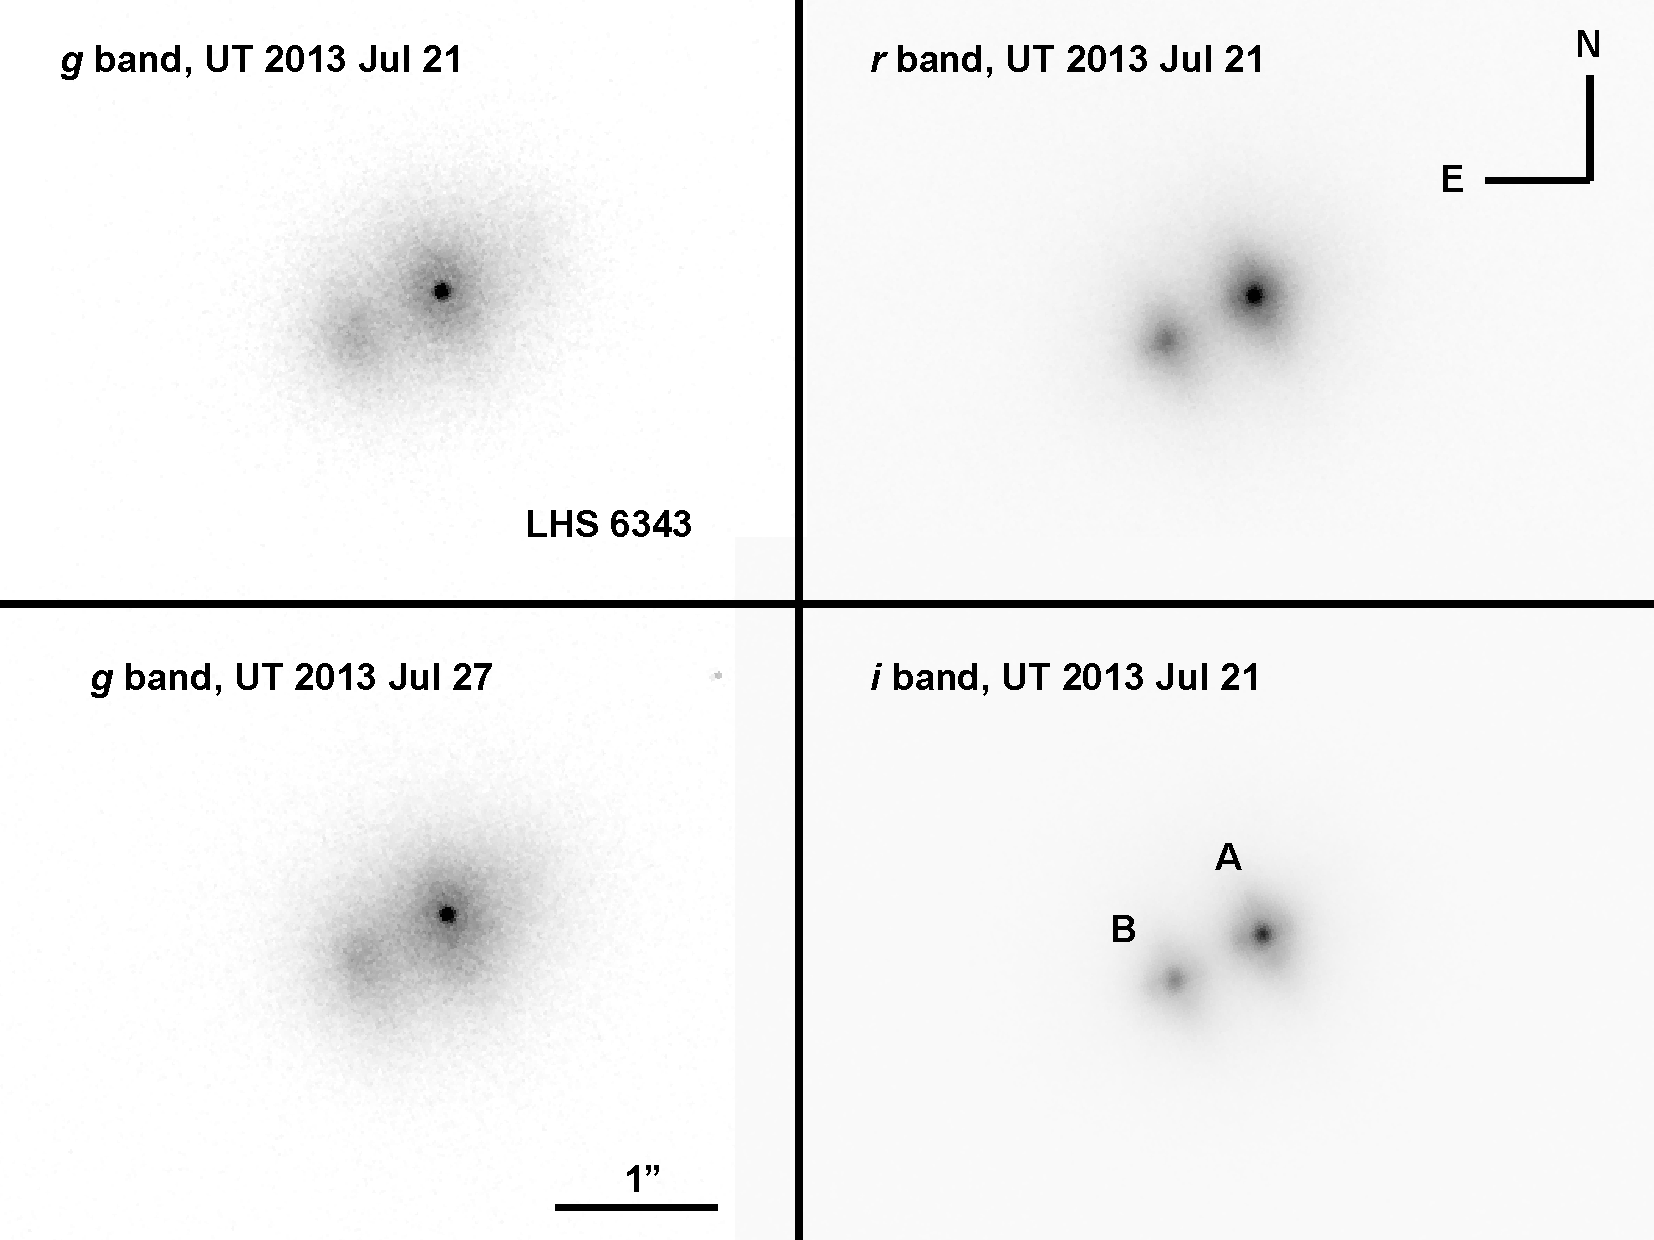
\includegraphics[width=0.85\textwidth]{chapter4/f1.pdf}}
\caption[Robo-AO adaptive optics imaging of the \LHS{} system]{Robo-AO adaptive optics imaging of the \LHS{} system taken with three different bandpasses.
Both the scale and orientation are held constant across all images.
We obtained two images of the system in the $g$-band, six days apart.
We obtained a single image of the system in both the $r$- and $i$-bands.
  }
\label{AOPlot}
\end{figure}


In our $g$-band data we observed tripling, induced when the shift-and-add processing algorithm temporarily locks on \LB{} instead of \LA.
Tripling causes the appearance of an artificial third object coaxial with the two real objects.
The third object is observed to have the same projected separation between the primary as the true secondary, at a position angle offset of 180 degrees, as discussed by \citet{Law06b}.
By measuring the flux ratios between the primary star and the two imaged companions, and defining $I_{jk} \equiv F_j/F_k$, then the true binary flux ratio $F_R$ is
\begin{equation}
F_R = \frac{2 I_{13}}{I_{12}I_{13} + \sqrt{I_{12}^2 I_{13}^2 - 4 I_{12} I_{13}}},
\end{equation}
where $F_1$ is the observed flux from the primary component, $F_2$ the observed flux from the secondary component, and $F_3$ the observed light from the tertiary, ``tripled'' component.
When $F_3 = 0$ this equation is undefined, but the asymptotic behavior is correct.

We find the third light contributions in each bandpass are given such that $\Delta g = 0.93 \pm 0.07$, $\Delta r = 0.74 \pm 0.06$, and $\Delta i = 0.57 \pm 0.05$.  
From these, we interpolate using the Dartmouth stellar models to calculate a value for the third light in the \itk{} bandpass, which encompasses roughly the $g$, $r$, and $i$ filters.
We find $\Delta K_p = 0.71 \pm 0.07$ magnitudes.
This is consistent with the extrapolation of J11, who predict a third-light in the \itk{} bandpass of $\Delta K_p = 0.74 \pm 0.10$. 


\subsection{NIR Spectroscopy}

The transit light curve itself can be used to measure some properties of \LA, such as the stellar density.
Other parameters such as the stellar temperature, as well as all physical properties of \LB, can only be estimated by relying on stellar models. 
To inform the models, on UT 2012 July 05 we obtained simultaneous JHK spectroscopy with the TripleSpec Spectrograph on the 200" Hale Telescope at Palomar Observatory. 
TripleSpec is a near-infrared slit spectrograph with a resolving power ($\lambda / \Delta \lambda$) of 2700 \citep{Wilson04, Herter08}. 

Observations were collected on four positions along the slit, ABCD, to minimize the effects of hot and dead pixels on the spectrograph detector. 
Each exposure was 30 seconds long in order to achieve a signal-to-noise ratio of 60.
We then observed a nearby, rapidly rotating A0V star to calibrate absorption lines caused by the Earth's atmosphere.

To reduce the data, we followed the methodology of \citet{Muirhead14}, using the SpexTool reduction package of \citet{Cushing04}. 
We differenced the A and B observations and the C and D observations separately, then extracted the combined-light spectrum and combined the separate observations with SpexTool. 
To remove the system's absolute radial velocity of -46 km s$^{-1}$, we cross-correlated the spectrum with data from the IRTF spectral library \citep{Cushing05, Rayner09}, then applied an offset to the wavelength solution corresponding to the peak of the cross-correlation function. 
The result is a single spectrum displaying the combined light from \LA{} and \LB, as shown in Figure \ref{TripleSpecPlot}

\begin{figure}[htbp!]
\centerline{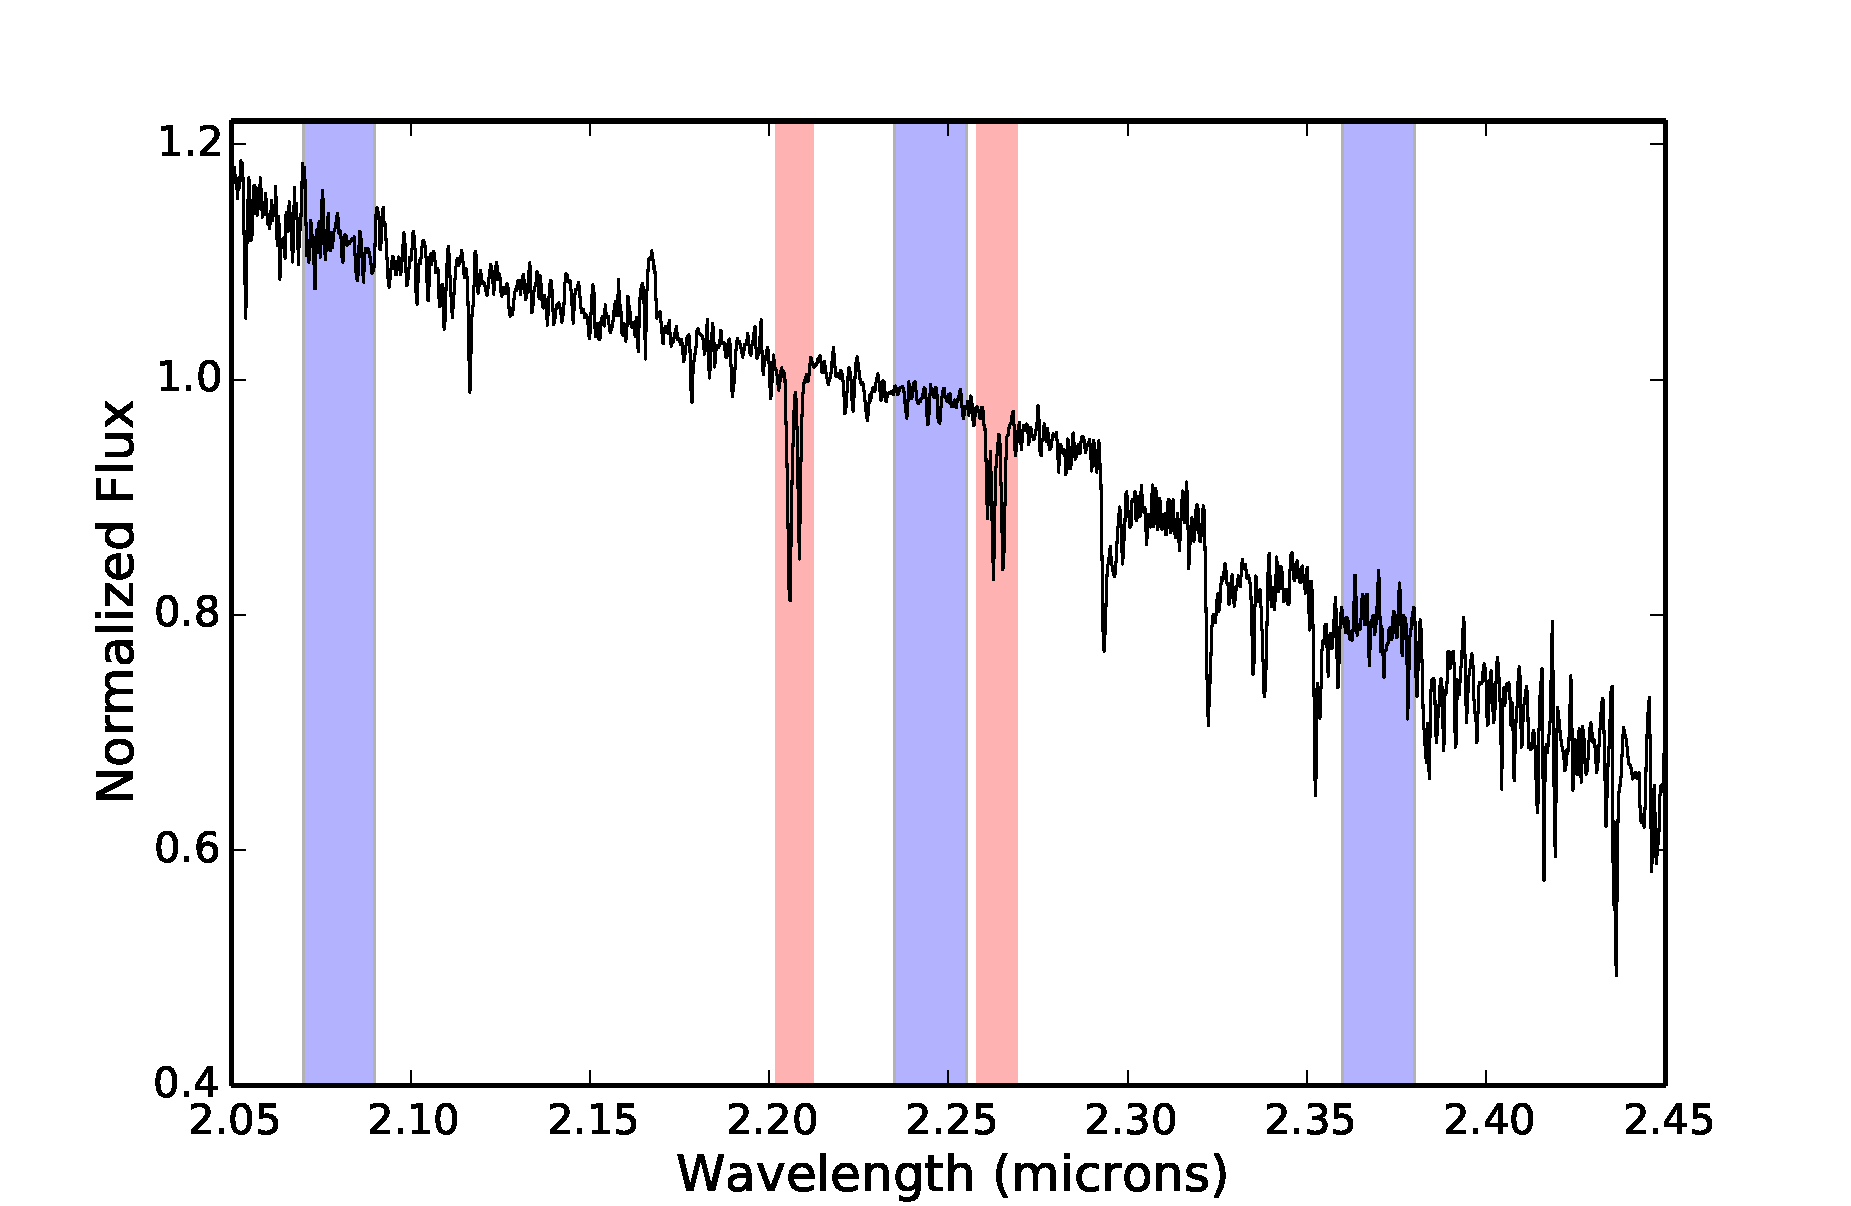
\includegraphics[width=0.75\textwidth]{chapter4/f2.pdf}}
\caption[Combined-light K-band spectrum for the \LHS{} system]{Combined-light K-band spectrum for the \LHS{} system.
The broad, blue shaded regions are used to derive the ``H$_2$O--K2 water index,'' as described in Section \ref{TripleSpec}.
The narrow, red shaded regions encompass the sodium doublet and calcium triplet.
Together, these regions have been used to develop empirical relations for the temperature and metallicity of M dwarfs \citep{RojasAyala12}.
  }
\label{TripleSpecPlot}
\end{figure}




\section{Data Analysis}

\subsection{Temperature and Metallicity of LHS6343\,A and B}
\label{TripleSpec}
We measured the temperature of each star following the method of \citet{RojasAyala12}, who built on the efforts of \citet{Covey10} to determine a relation between K-band spectroscopic features and the temperature and metallicity of M dwarfs. 
Specifically, Rojas-Ayala et al. define a temperature-sensitive ``H$_2$O--K2 water index," representing the water opacity between 2.07 $\mu$m and 2.38$\mu$m:
\begin{equation}
\textrm{H}_2\textrm{O--K}2 = \frac{\langle\mathcal{F}(2.070-2.090)\rangle /\langle\mathcal{F}(2.235-2.255)\rangle}{\langle\mathcal{F}(2.235-2.255)\rangle /\langle\mathcal{F}(2.360-2.380)\rangle}.
\end{equation}
Here, $\langle \mathcal{F}(a-b)\rangle$ represents the median flux level in the region $[a, b]$, with both $a$ and $b$ in $\mu$m.
They also defined a relation between a star's metallicity, the H$_2$O--K2 index, and the equivalent width of the 2.21 $\mu$m sodium doublet and 2.26 $\mu$m calcium triplet. 
We calculated H$_2$O--K2 and the two equivalent widths, as well as their uncertainties, by creating a sequence of simulated spectra in which random noise is added to the observed flux consistent with the flux uncertainty at each wavelength.
We found the calculated H$_2$O--K2 values to be normally distributed such that H$_2$O--K2 $ = 0.919 \pm 0.002$. 
The equivalent width of the sodium doublet is $5.533 \pm 0.101$ \AA{} and the equivalent width of the calcium triplet is $3.863 \pm 0.089$ \AA.

If our spectrum consisted of the flux from only one star, we could convert our value directly into a stellar effective temperature and metallicity. 
In this case, each value is really the combination of two separate values, one for each M dwarf. 
However, if we assume the two stars have the same metallicity, useful information can still be extricated.
We first drew from the posterior of $\Delta K$ values from our PHARO near-infrared adaptive optics observations and our posteriors for H$_2$O--K2 and the equivalent widths. 
From these, we used the relations of \citet{RojasAyala12} to calculate the system metallicity. 
We then interpolated the table provided in that paper to find a relation between H$_2$O--K2 and effective temperature for a given metallicity. 
Using the Dartmouth stellar evolution models, we then determined which two modeled stars best fit both the observed flux ratio and combined H$_2$O--K2 index value. 
By repeating this process many times, continuously drawing from the posteriors for each measured value we determined a posterior on the temperature, and by extension the mass, of each star. 
The joint posterior on the temperature of the two stars is shown as Figure \ref{TempPlot}.

\begin{figure}[htbp]
\centerline{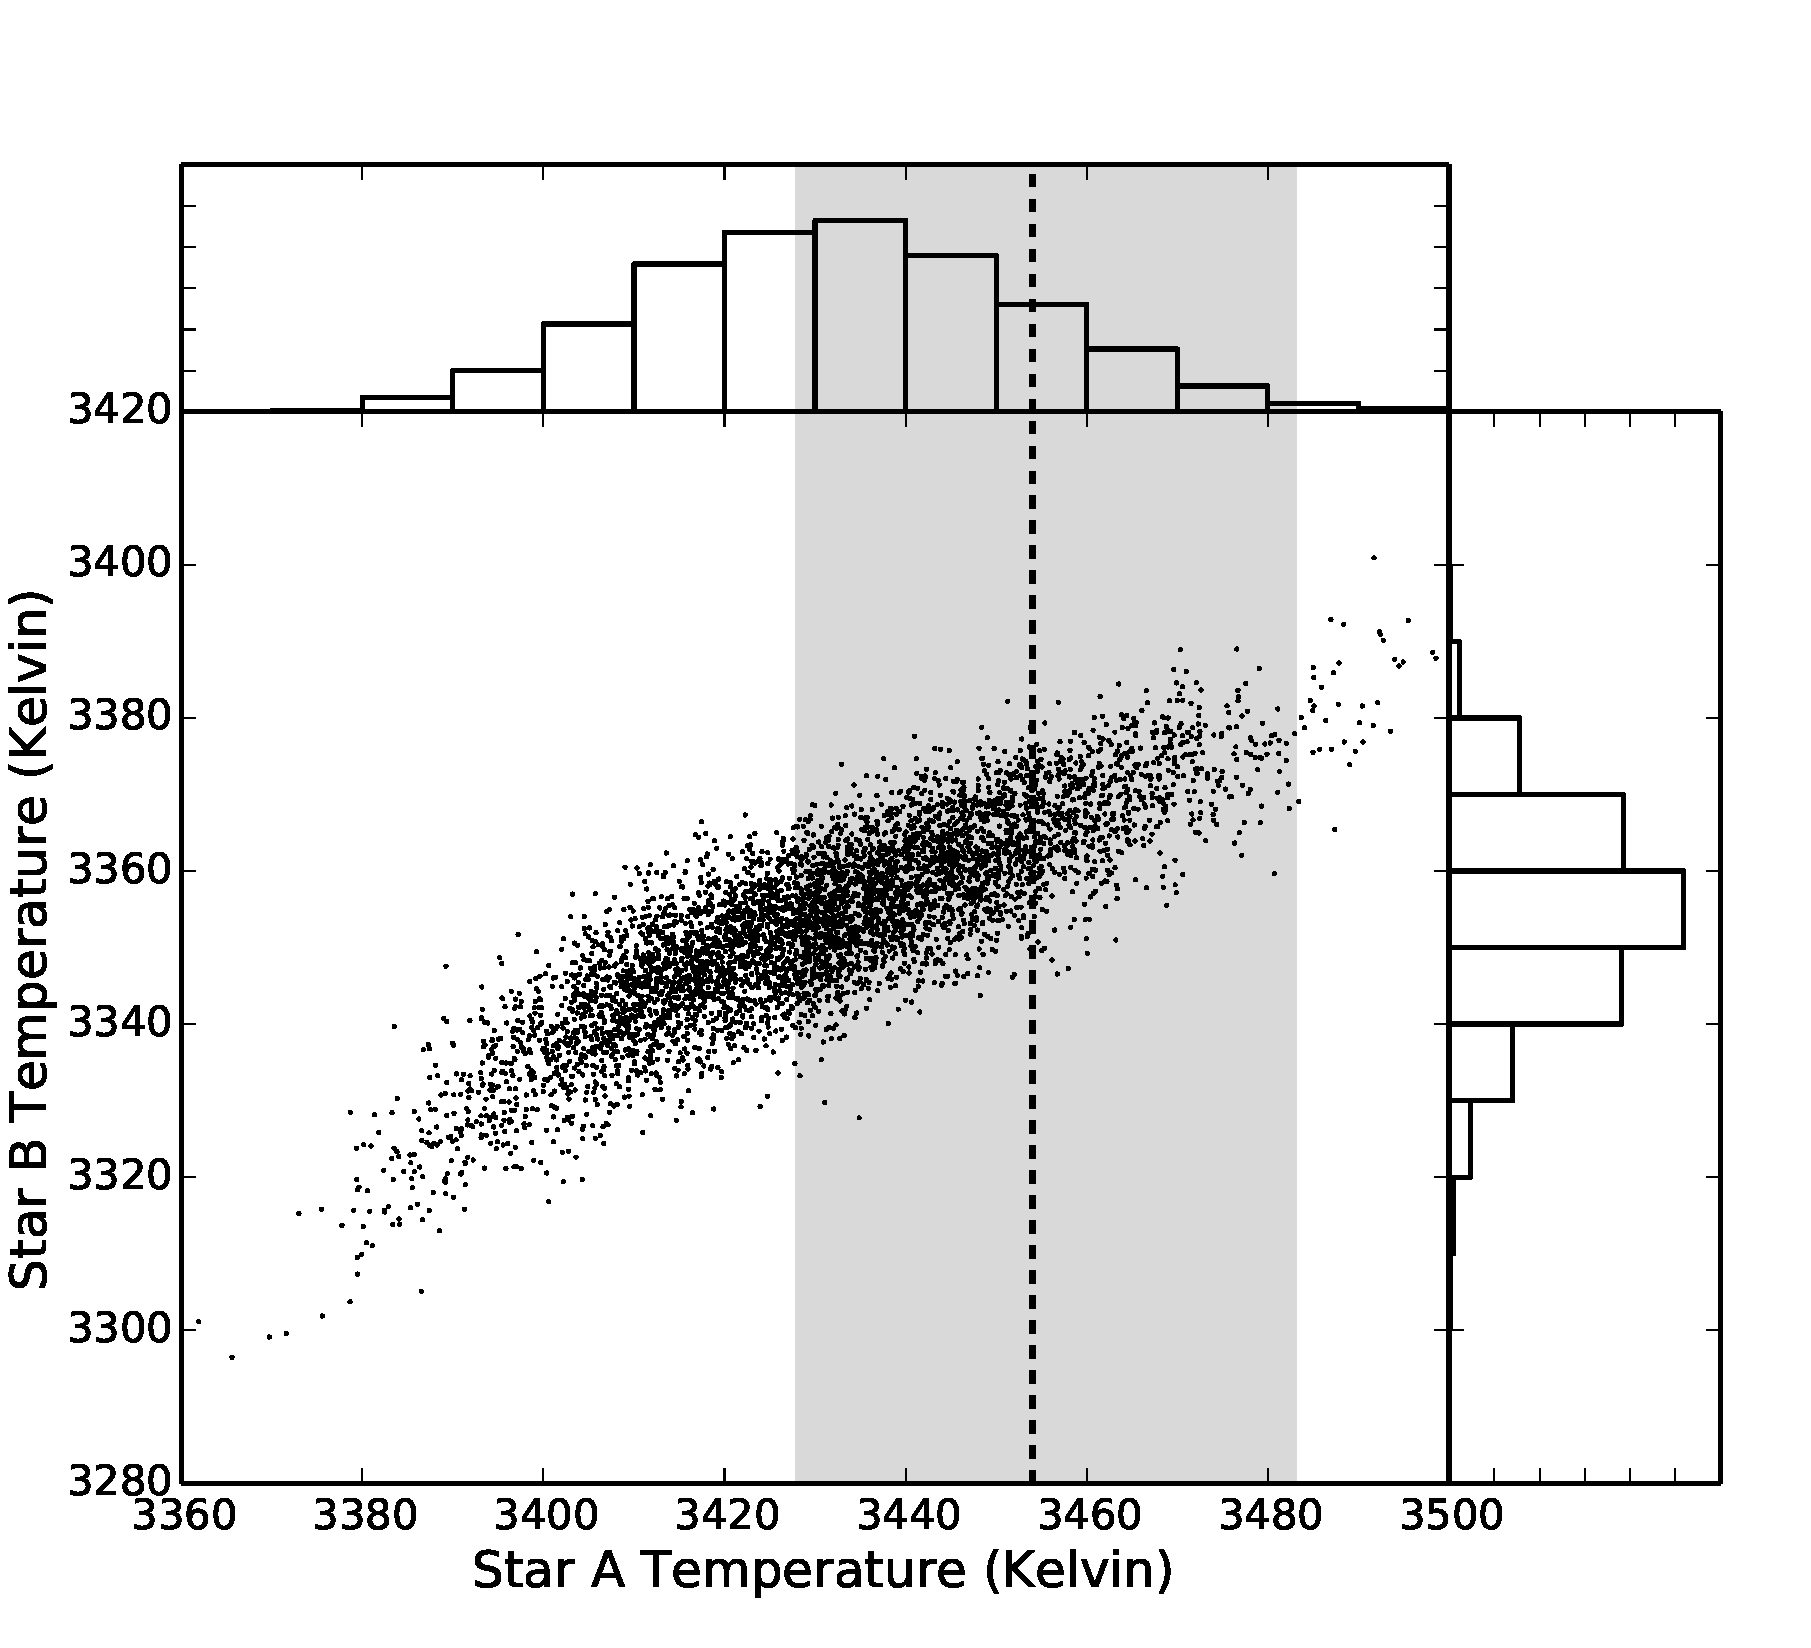
\includegraphics[width=0.75\textwidth]{chapter4/f3.pdf}}
\caption[Joint posterior on the effective temperature of \LA\ and B]{Joint posterior on the effective temperature of \LA{} and \LB. 
Marginalizing over the temperature of each star separately, we find the A component has a temperature of $3431 \pm 21$ K and the B component has a temperature of $3354 \pm 17$ K. The dashed line and shaded region correspond to the temperature of \LA{} expected based on our model-independent mass measurement from the combined transit and RV fit.
}
\label{TempPlot}
\end{figure}





\subsection{Transit Parameters}

To measure the parameters of \LC, we forward modeled the \LA-C system over the timespan from the launch of \itk{} to the date of the final RV observation in 2013.
At each time corresponding to an RV observation, we calculated the expected radial velocity relative to a stationary \LB{} assuming a Keplerian orbit.
At each \itk{} timestamp during a transit or near the expected time of secondary eclipse, we calculated the expected relative flux assuming a \citet{Mandel02} light curve model. 
We fit four limb darkening parameters using the prescription of \citet{Claret11}, allowing the value for each limb darkening coefficient to float as a free parameter. 
In calculating the light curves, we used an adapted version of the PyAstronomy package\footnote{https://github.com/sczesla/PyAstronomy}, modified to allow eccentric orbits.

In all, we fit for 16 parameters: $\sqrt{e}\cos\omega$, $\sqrt{e}\sin\omega$, time of central transit, orbital period, brown dwarf mass, orbital inclination, \LA-C radius ratio, four limb darkening parameters, the third light from \LB, \logg{} of \LA, the secondary eclipse depth, the stellar mass, and the RV zeropoint (relative to \LB). We did not use an RV jitter term, as our RV uncertainties of $\sim 100$ m s$^{-1}$ are significantly larger than the jitter expected for a main-sequence M dwarf. We used {\texttt emcee}, an affine-invariant ensemble sampler described by \citet{Goodman10} and implemented by \citet{Foreman-Mackey12}, to maximize the likelihood function
\begin{eqnarray}
\mathcal{L} &=& 0.5 \bigg[\sum_i \bigg(\frac{\textrm{RV$_{\textrm{model, $i$}}$} - \textrm{RV$_{\textrm{observed, $i$}}$}}{\sigma_{\textrm{RV}, i}}\bigg)^2 \nonumber \\
&+& \sum_i
 \bigg(\frac{f_{\textrm{model SC, $i$}} - f_{\textrm{observed SC, $i$}}}{\sigma_{f _\textrm{SC}, i}}\bigg)^2 \nonumber \\
 &+& \sum_i
 \bigg(\frac{f_{\textrm{model LC, $i$}} - f_{\textrm{observed LC, $i$}}}{\sigma_{f _\textrm{LC}, i}}\bigg)^2\bigg].
\end{eqnarray}
Here, $f_\textrm{LC}$ corresponds to the observed flux in the \itk{} long cadence data and $f_\textrm{SC}$ corresponds to the short cadence data.
The period we fit and report here is the period observed in the frame of an observer at the barycenter of the solar system, not in the frame of the \LHS{} system.
That is, we do not correct for relativistic effects induced by the star system's systemic velocity.

We imposed two different priors on the stellar mass, reflecting various levels of trust in theoretical stellar evolutionary models. 
First we apply the stellar empirical mass-radius relation of \citet{Boyajian12}, which encodes no direct model-dependent information, as a prior
We use their relation for ``single stars.''
While our star has a wide binary companion at tens of AU, the single collection is more representative of \LA{} than the short-period eclipsing binaries used to build the eclipsing binary main sequence of \citet{Boyajian12}.
Given a precise measurement of the stellar density \rhostar, semimajor axis $a/$\rstar, Doppler semiamplitude $K$, eccentricity, and inclination, the mass and radius of both the primary and secondary star can then be calculated.


We next repeated this analysis, applying a prior on the stellar mass using the spectroscopic parameters from our TripleSpec analysis, as described in Section {\ref{TripleSpec}}.



In each of these cases, we can calculate the mass and radius of \LB{} through the Dartmouth models by comparing the relative brightness of \LA{} and \LB{} in conjunction with the (now known) mass of \LA. 
We can also measure a model-dependent distance to the system, which depends both on our measured mass and the mass-luminosity relation encoded in the stellar models.

The best fit model to the light curve data and RVs are plotted in Figures \ref{LC} and \ref{RVs-4}, respectively.


\begin{figure}[htbp]
\centerline{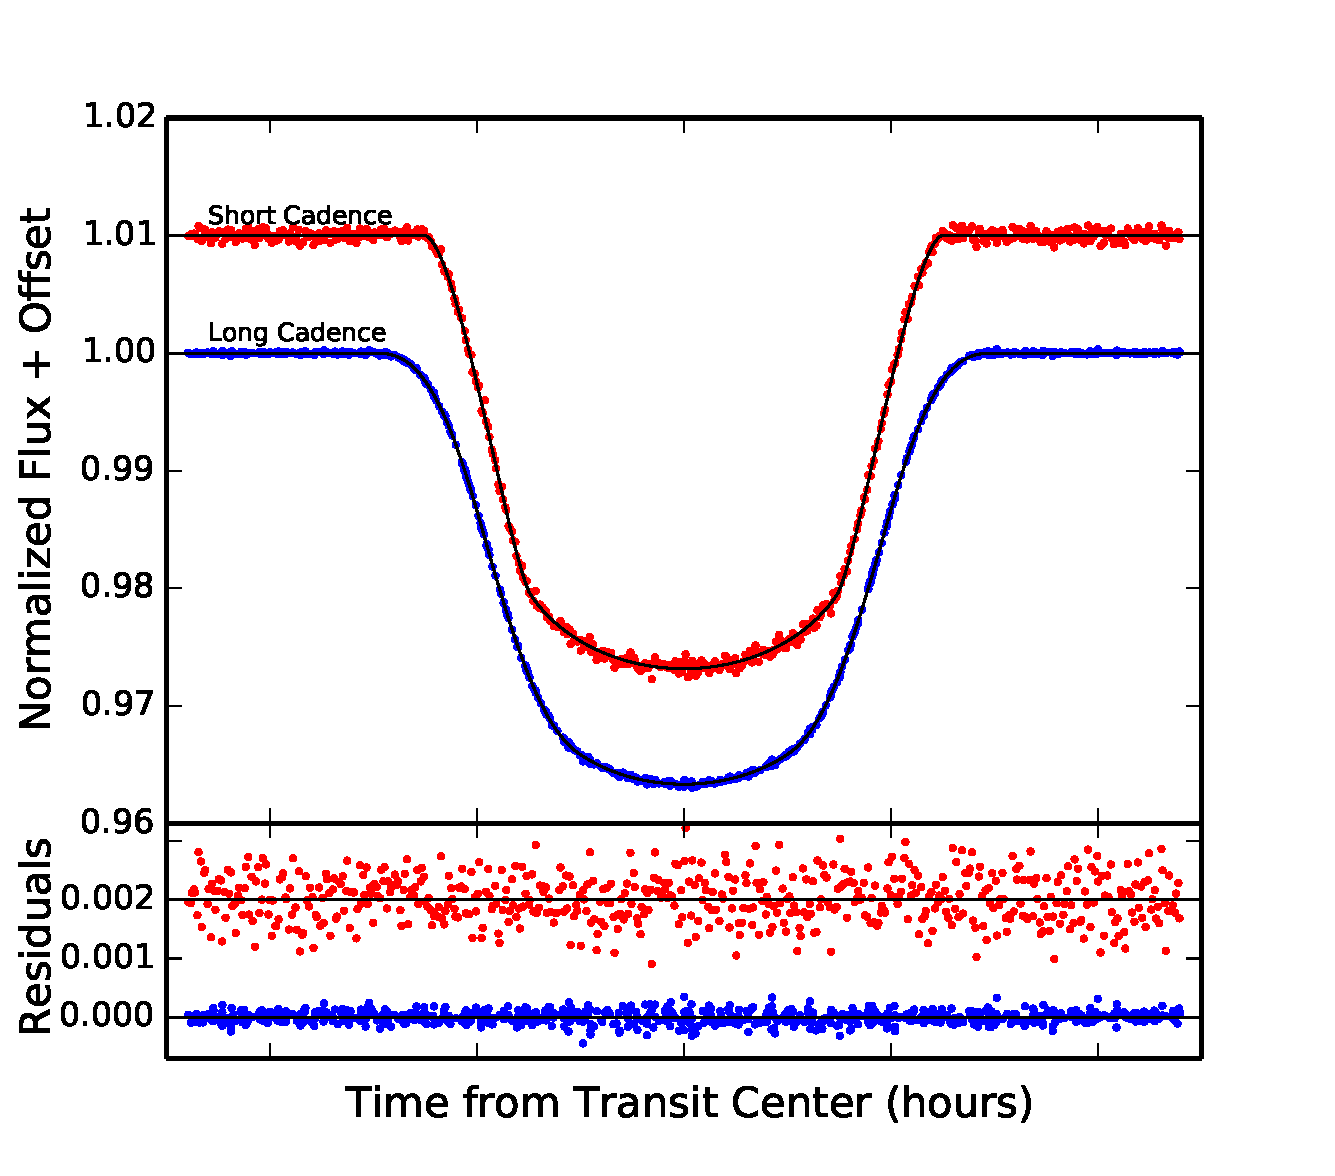
\includegraphics[width=0.75\textwidth]{chapter4/f4.pdf}}
\caption[Phase-folded transit light curve, fit to the maximum likelihood model]{Phase-folded transit light curve, fit to the maximum likelihood model.
Blue points represent long cadence data and red points represent short cadence data.
The scale of the residuals is a factor of five larger than the scale of the light curve.
  }
\label{LC}
\end{figure}


\begin{figure}[htbp]
\centerline{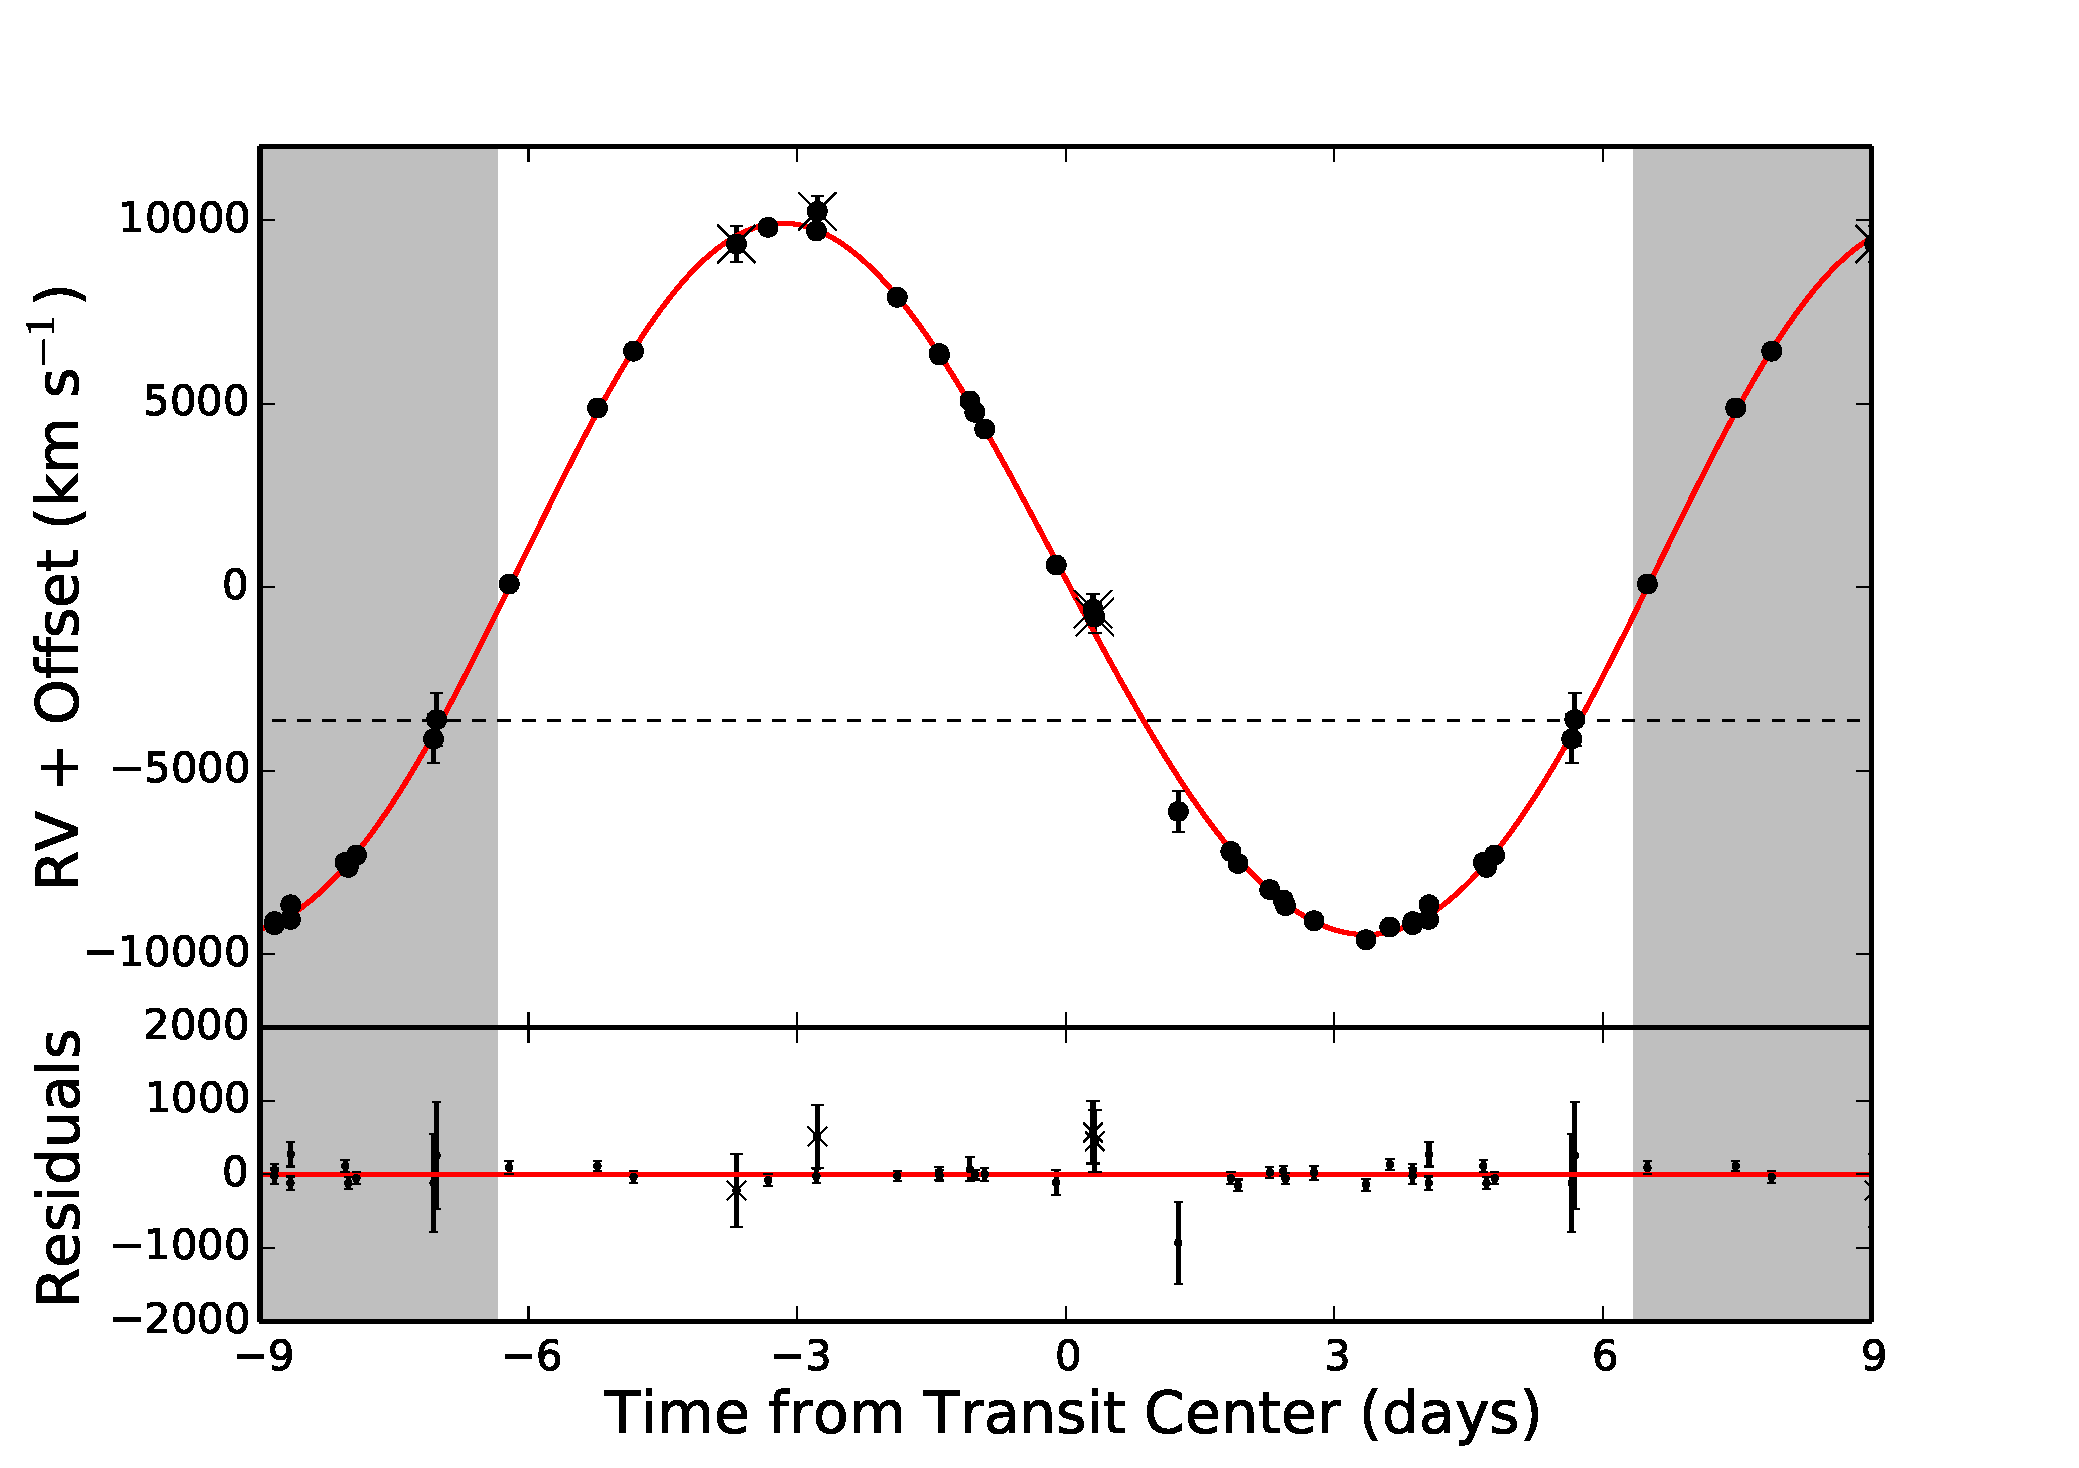
\includegraphics[width=0.75\textwidth]{chapter4/f5.pdf}}
\caption[Phase-folded RV curve, fit to the maximum likelihood model]{Phase-folded RV curve, fit to the maximum likelihood model.
For the majority of observations, the data points are larger than the size of the error bars.
The gray shaded regions represent an extension of the RV data beyond one phase to provide clarity for the reader. 
Observations marked with an cross represent data collected while using the iodine cell.
The dashed line represents the RV of \LB{}, which does not change at the level of our precision over the 3-year RV baseline.
  }
\label{RVs-4}
\end{figure}



\section{Results}

The orbital parameters for \LC{} are listed in Table \ref{OrbitTable}.
The physical properties of the \LHS{} system are listed in Table 4.3. 
In the latter table, we include two columns of values. 
The first set of values represents the values we find using our data-driven model, using only the empirical mass-radius relation of \citet{Boyajian12} without any direct use of stellar models. 
The second set of values corresponds to the inclusion of a model-dependent prior on the stellar mass.
In this case, we impose as a prior our mass derived from the near-IR spectroscopy, found in Section {\ref{TripleSpec}}.

We find that we are able to measure the observed transit depth, uncorrected for the third light contributions of \LB, to a precision of 0.5\%.
We are additionally able to measure the Doppler semiamplitude $K$ to 0.3\%. 
Therefore, our uncertainties in the brown dwarf's physical parameters are dominated by the uncertainties on the absolute physical parameters of the two M dwarfs in the system.

We can measure the stellar mass directly from the light curve and RV observations without any direct reliance on theoretical stellar models, as shown in the Discussion.
In this case, we measure a mass for \LA{} of $0.381 \pm 0.019$ \msun{} and a radius of $0.380 \pm 0.007$ \rsun.  
We then find a mass and radius of \LC{} of $64.6 \pm 2.1$ \mjup{} and $0.798 \pm 0.014$ \rjup, respectively.
Thus, in this case we can measure the mass of the brown dwarf to a precision of $3.2\%$ and the radius to $1.8\%$. 

From our near-IR spectroscopic analysis of the system, we measure a temperature for \LA{} of $3431 \pm 21$ K, which gives us a mass of $0.339 \pm 0.016$ \msun. 
We repeat our analysis, using this value as a prior on our stellar mass.
In this case, we find a value for the stellar mass between our empirical value and that imposed by our model prior: $0.358 \pm 0.011$ \msun.
We then find a mass for the brown dwarf of $62.1 \pm 1.2$ \mjup{} and a radius of $0.782 \pm 0.013$ \rjup. 
This is a model-dependent mass measured to a precision of $1.9\%$ and a model-dependent radius to $1.4\%$. 

Our brown dwarf mass is consistent with that found by J11, while our radius is smaller at the $1.4\sigma$ level. 
Part of this discrepancy may be due to the choice of models used: these authors used the Padova model grids of \citet{Girardi02}. 
These models predict a larger mass than both the Dartmouth models we use and the BT-Settl models \citep{Allard10}.
Using the Padova models, the authors of the discovery paper adopted a slightly smaller \logg, which for a given mass implies a larger star, and therefore a larger planet.
The discrepancy may also be affected by our choices of limb darkening models: the authors of the discovery paper use a quadratic limb darkening model.
With only five transits observed, this is a reasonable choice. 
Given the signal to noise obtained from fitting four years of \itk{} data simultaneously, we require a four-parameter limb darkening solution to develop an appropriate model fit.

Our mean density for \LC{} is 40\% larger than that reported in the discovery paper.
This appears to be because the authors of that paper misreported their density, as it is inconsistent with their reported mass and radius. 
These authors may have reported the density relative to Jupiter, not in units of g cc$^{-1}$ as listed in their Table 5.
Even with this correction, the density we report is larger than the density of J11 due to the difference in the radius of the brown dwarf described in the previous paragraph.

We measure a period of $12.7137941 \pm 0.0000002$ days in the frame of the solar system. 
The uncertainty in the period is 17 milliseconds, and the period is measured to a precision of 15 parts per billion.

We measure the total mass in the \LA C system to a precision of 4.8 percent. 
Neglecting our uncertainty in the measured period, from differentiating Kepler's Third Law we expect our measurement of the semimajor axis to be three times more precise than that of the total mass.
In fact, we measure a semimajor axis of $0.0812 \pm 0.0013$ AU, a precision of 1.6 percent.


\subsection{Secondary Eclipse Observation}

J11 do not detect a secondary eclipse and can only place an upper limit of 65 parts per million on the potential eclipse depth.
With a full four years of \itk{} data, we are considerably more sensitive to eclipses.
From the RVs and shape of the primary eclipse alone, we know the A-C system has a nonzero eccentricity: we find $e \cos \omega = 0.024 \pm 0.003$.
As a result, we expect the secondary eclipse to occur approximately 4.5 hours after the midpoint between consecutive primary transits. 

When we include a secondary eclipse in our system model, we detect a signal at $3.5\sigma$, as shown in Figure \ref{SecondaryPlot}.
This eclipse has a depth of $25 \pm 7$ parts per million and occurs $4.44 \pm 0.16$ hours after the midpoint between primary transits.
From these data, we measure $e \cos \omega = 0.0228 \pm 0.0008$.


\begin{figure}[htbp]
\centerline{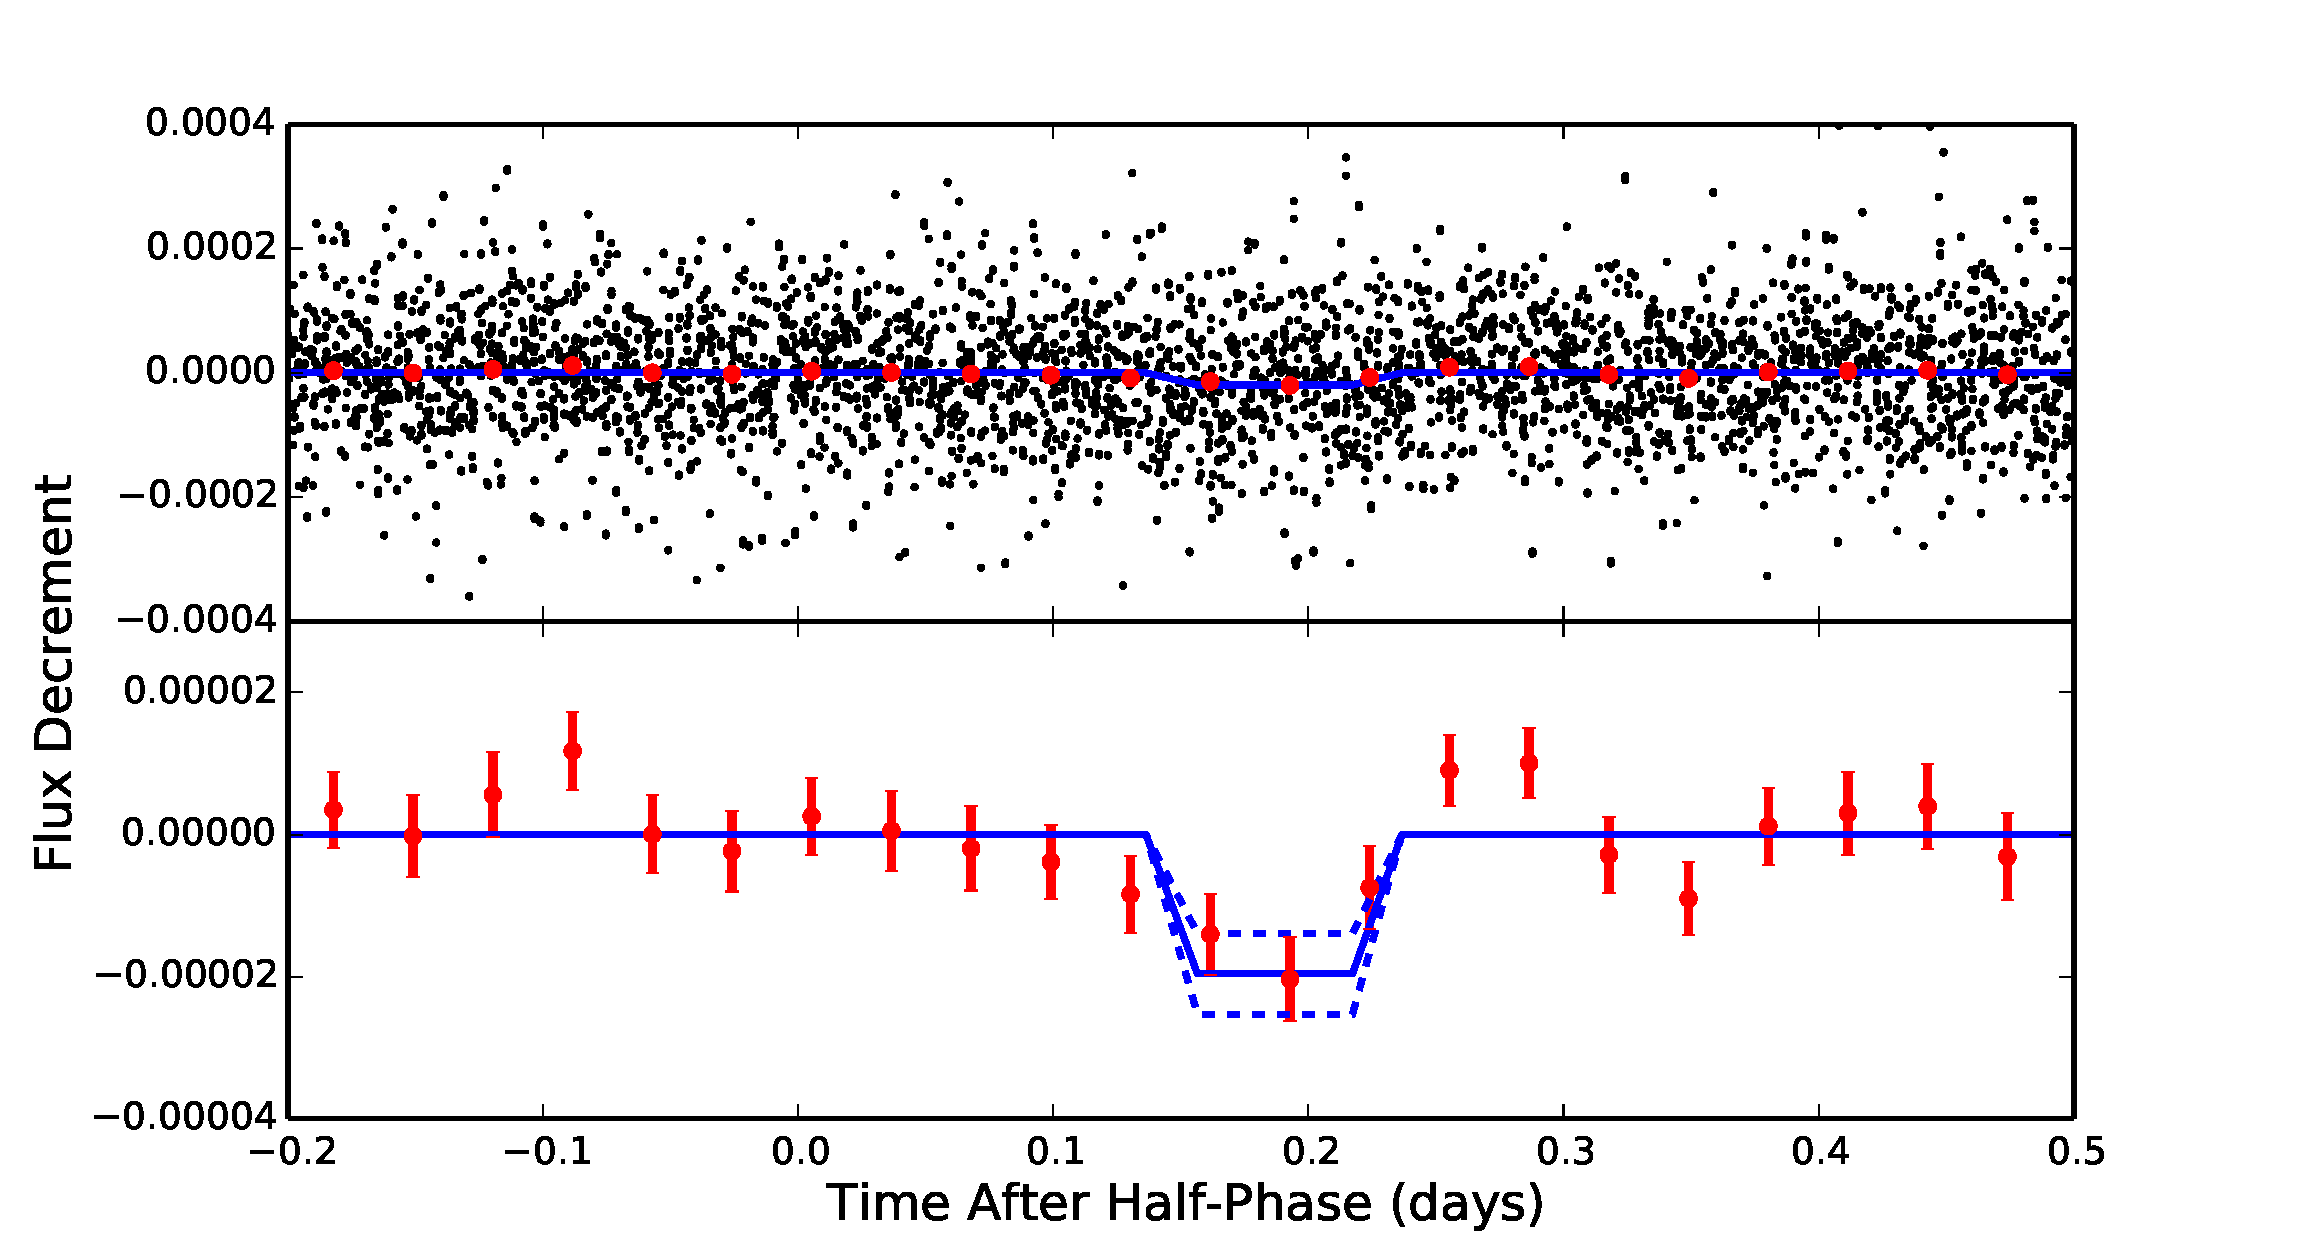
\includegraphics[width=0.75\textwidth]{chapter4/f6.pdf}}
\caption[Secondary eclipse of \LC{} as observed by \itk]{Secondary eclipse of \LC{} as observed by \itk. 
(top) In black, the \itk{} data are phase-folded and plotted; we bin every 0.03 days of observations together to reduce the apparent scatter, as shown in red. 
As the noise is nearly completely white, this is justified for plotting purposes.
In blue is our best-fitting secondary eclipse model.
We treat the brown dwarf as a uniform sphere in our modeling efforts.
(bottom) Same as the above, excluding the raw data. 
We detect an eclipse depth of $25 \pm 7$ ppm after accounting for the correction for the third light contribution from \LB.
The dashed blue lines represent the $1\sigma$ deviation in eclipse depth from the best-fitting model.
}
\label{SecondaryPlot}
\end{figure}




\subsection{Distance to the \LHS{} System}

There is, at present, no measured parallax to the \LC{} system. 
We must therefore rely on stellar models to convert the measured apparent magnitudes to distance estimates.
J11, using the Padova model atmospheres, announced a distance to the system of $36.6 \pm 1.1$ pc. 
The Dartmouth models predict a lower mass, and therefore a lower luminosity for \LA{}, so to maintain the observed brightness of the system from $g$ to $K_s$-band, these models require a smaller distance modulus.
We find a model-dependent distance to the system of $32.7 \pm 1.3$ pc.
A measured parallax to this system, either from the ground or from Gaia, will be useful for resolving the $2\sigma$ discrepancy between these distances, informing the upcoming next generation of stellar evolution models.

\begin{table}[hbt!]
\centering
\begin{tabular}{lccc}
\hline
\footnotesize
Parameter & 
Value    &
 &
$1\sigma$ Confidence \\
 & & & Interval \\
\hline
Orbital Period, $P$~[days] & 12.7137941 & $\pm$& 0.0000002 \\
Transit Center (TDB $- 2440000$) & 15008.07259 & $\pm$ &  0.00001 \\
Radius Ratio, $(R_P/R_\star)$ &      0.216 & $\pm$ &       0.004 \\
Observed Transit Depth (percent) &  3.198 & $\pm$ &       0.015 \\
Scaled Semimajor axis, $a/R_\star$  &  46.0 & $\pm$ &       0.4 \\
Orbital Inclination, $i$~[deg] &  90.45 & $\pm$ &     0.03  \\
Transit Impact Parameter, $b$ &  0.36 & $\pm$ &     0.02 \\
Argument of Periastron $\omega$~[degrees] & -40 & $\pm$ &      4 \\
Eccentricity  &  0.030 & $\pm$ &      0.002  \\
Secondary Phase ($e \cos \omega$) & 0.0228 & $\pm$ &      0.0008 \\
Secondary Depth (ppm) & 25 & $\pm$ & 7 \\
Velocity semiamplitude $K_A$~[km s$^{-1}$] &  9.69 & $\pm$ &       0.02 \\
Star A-B RV Offset [km s$^{-1}$] & 3.64 & $\pm$ &       0.02  \\
\hline
\end{tabular}
\caption[Orbital Parameters for the LHS\,6343\,AC System]{Orbital Parameters for the LHS\,6343\,AC System. All parameters calculated by simultaneously fitting to the RV data and \itk{} data near the times of transit and secondary eclipse.}
\label{OrbitTable}
\end{table}

\begin{landscape}
\begin{table}[hbt!]
\footnotesize
\begin{center}
\begin{tabular}{lccccccc}
\hline
Parameter & Value &  & $1\sigma$ Confidence & Value & $1\sigma$ Confidence & Comment \\
  & (Empirical Prior) & & Interval & (Model Prior) & & Interval & \\
\hline
\emph{Stellar Parameters} & & & \\
$M_A$~[\msun] &  0.381 & $\pm$ &       0.019 &      0.358 & $\pm$ &      0.011 & A \\
$M_B$~[$M_\odot$] & & & & 0.292 & $\pm$ & 0.013 & A \\
$R_A$~[$R_\odot$] &   0.380 & $\pm$ &       0.007 &      0.373 & $\pm$ &      0.005 & A \\
$R_B$~[$R_\odot$] & & & & 0.394 & $\pm$ & 0.012 & A \\
$\rho_A$~[$\rho_\odot$] & 6.96 & $\pm$ &       0.19 &      6.93 & $\pm$ &      0.19 & A \\
$\log g_A$~[cgs] &  4.86 & $\pm$ &        0.01 &       4.85 & $\pm$ &       0.01 & A \\
Metallicity [Fe/H] & & & & 0.03 & $\pm$ & 0.26 & B \\
Metal Content [a/H]  & & & & 0.02 & $\pm$ & 0.19 & B \\
Distance~[pc] & & & & 32.7 & $\pm$ & 1.3 & C \\
Flux Ratio $F_B/F_A, K_p$ &   0.461 & $\pm$ &       0.055 &      0.518 & $\pm$ &    0.032 & A \\
$\Delta K_p$ [magnitudes] & 0.84 & $\pm$ & 0.12 & 0.71 & $\pm$ & 0.07 & A \\
$T_{{\textrm eff}, A}$ [K] & & & & 3431 & $\pm$ & 21  & B\\
$T_{{\textrm eff}, B}$ [K] & & & & 3354 & $\pm$ & 17  & B\\
 & & \\
\emph{Brown Dwarf Parameters} & & & \\
$M_C$~[\mjup] & 64.6 & $\pm$ &        2.1 &      62.1 & $\pm$ &       1.2 & A \\
$R_C$~[\rjup] & 0.798 & $\pm$ &       0.014 &      0.783 & $\pm$ &      0.011  & A\\
Semimajor Axis, A-C System (AU) &  0.0812 & $\pm$ &      0.0013 &     0.0797 & $\pm$ &     0.0008 & A \\
Mean Planet Density, $\rho_C$~[g cm$^{-3}$] & 170 & $\pm$ &       5. &    173 & $\pm$ &      5 & A \\
$\log g_C$~[cgs] &  5.419 & $\pm$ &       0.008 &      5.420 & $\pm$ &      0.008 & A \\
$T_{\textrm eq}$ ($T_{\textrm eff}(\frac{R_\star}{2a})^{1/2}$)~[K] & & & & 358 & $\pm$ & 3 & A,B \\
\hline
\end{tabular}
\caption[Physical Parameters for LHS\,6343\,ABC]{Physical Parameters for LHS\,6343\,ABC. \\
(A) Calculated by simultaneously fitting to the RV data and \itk{} data near the times of transit and secondary eclipse. \\
(B) Measured from near-IR spectroscopy following the method of \citet{RojasAyala12}. \\
(C) Calculated by fitting the observed apparent magnitudes to model-predicted absolute magnitudes.
}
\end{center}
\label{BigTable}
\end{table}
\end{landscape}
\clearpage




\section{Discussion}

\begin{figure}[htbp]
\centerline{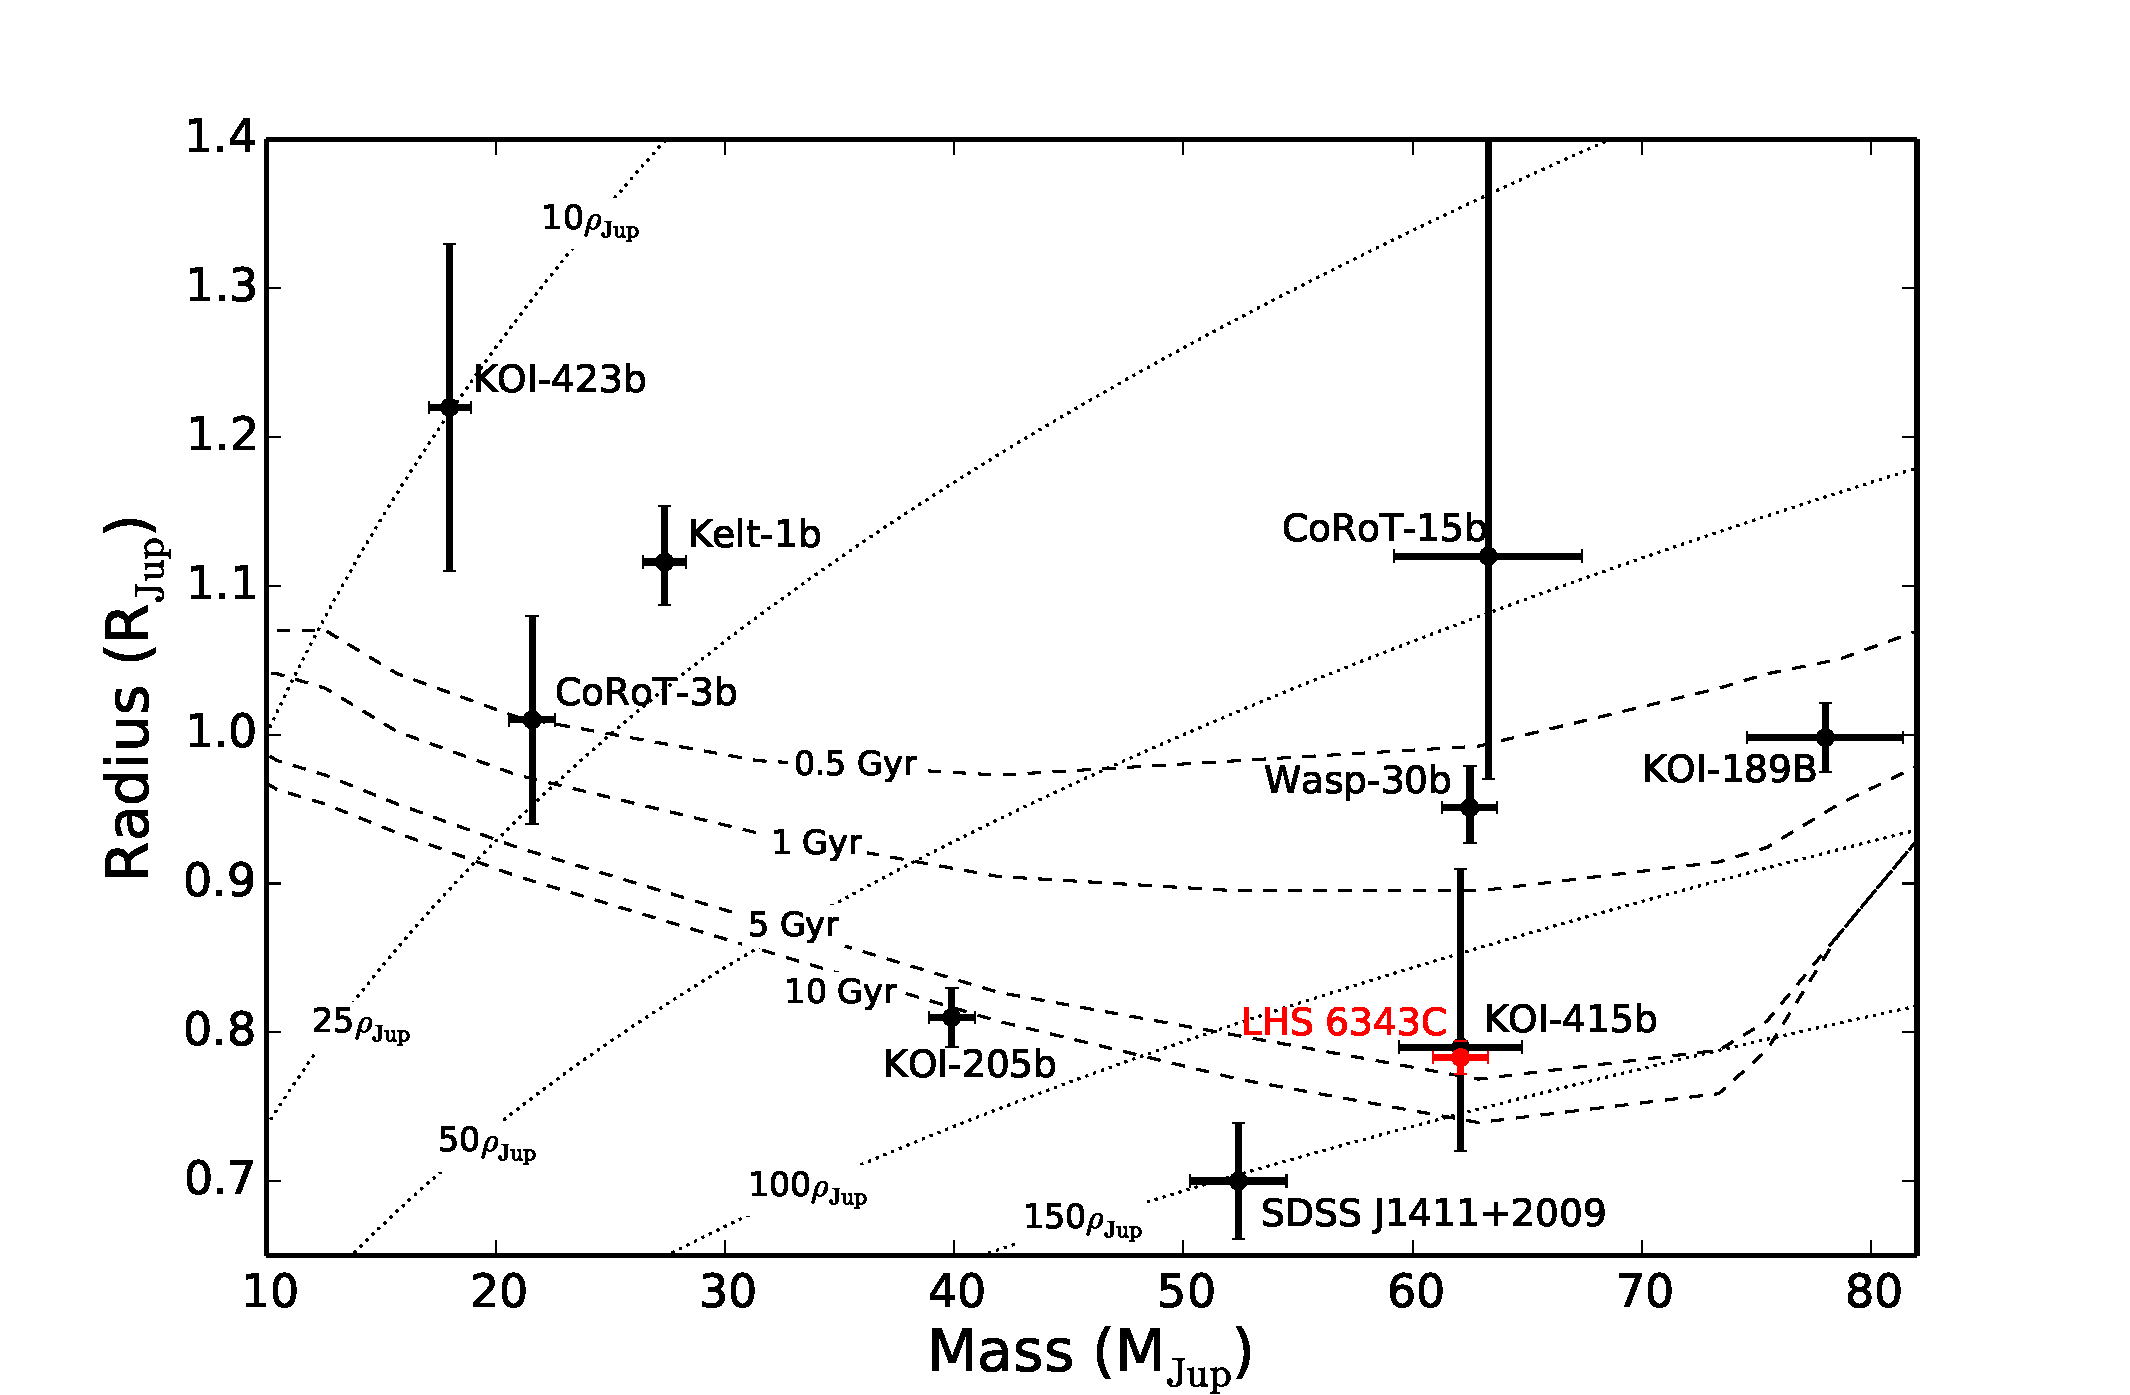
\includegraphics[width=0.75\textwidth]{chapter4/f7.pdf}}
\caption[Mass-radius diagram for known transiting brown dwarfs]{Mass-radius diagram for known transiting brown dwarfs.
The dashed lines represent the \citet{Baraffe03} isochrones for (top to bottom) ages of 0.5, 1.0, 5.0, and 1.0 billion years.
The dotted lines are isodensity contours for (top left to bottom right) densities corresponding to 10, 25, 50, 100, and 150 times the density of Jupiter. 
\LC{} has a density of $130 \pm 4 \rho_\textrm{Jup}$ and appears to have an age of 3-5 Gyr.
Data taken from \citet{Deleuil08, Bouchy11a, Bouchy11b, Siverd12, Diaz13, Moutou13, Triaud13, Diaz14b, Littlefair14}.
Not shown are the components of the young binary brown dwarf system
2MASS 2053-05 \citep{Stassun06}, which have
radii well above the plot range.
  }
\label{MassRadiusPlot}
\end{figure}


There are now nine brown dwarfs with measured masses and radii \citep{Moutou13}. 
Of this sample, there are only four that are not inflated due to youth or irradiation.
\LC{} is effectively a field brown dwarf: the equilibrium temperature for an object at its orbital separation is 360 K while a 65 \mjup{} brown dwarf is expected to cool to only 700 K over a Hubble time \citep{Burrows01}.
Thus, the irradiation from the primary star on the brown dwarf is negligible.
Additionally, since the system has a nonzero eccentricity, the system is not tidally locked, minimizing any effects the primary star may have on any one point on the brown dwarf's surface.
\LC{} can be used as a laboratory to study the physics of solitary brown dwarfs, as it is effectively a field brown dwarf with a known mass, radius, and metallicity.
The sample of transiting brown dwarfs that can be used to probe the physics of field brown dwarfs is highly limited, making each individual system extremely valuable.

There is some evidence that our current best understanding of the physics of brown dwarfs is incomplete.
\citet{Dupuy09} find evidence for a ``substellar luminosity problem,'' in which the brown dwarf binary HD\,130948\,BC is twice as luminous as predicted by evolutionary models.
A similar result is found in the Gl 417 BC system \citep{Dupuy14}.
As these are the only two brown dwarf systems with reliable measurements of both mass and age, this result is suggestive of a fundamental issue with substellar models.

We have only a lower limit on the age of the system: J11 find no youth indicators present in the \LHS{} system so it is likely not less than 1-2 Gyr old.
Therefore, a measured luminosity would be most useful as a probe of this specific plane if the luminosity were consistent with extreme youth ($< 1$ Gyr) or extreme age ($>14$ Gyr).
A measured luminosity is still useful, as it allows us to locate the brown dwarf's position in the mass-radius-luminosity plane. 
While there is a collection of non-inflated brown dwarfs with masses and luminosities measured, there are only three with mass and radius and none with both radius and luminosity.
Moreover, we also know the metallicity of the brown dwarf, assuming it has the same composition as \LA B. 

There is a degeneracy between the inferred age of the system and the atmosphere of the brown dwarf.
Specifically, a brown dwarf with the mass and radius of \LC{} would be expected to be significantly older if it were covered with optically-thick clouds, as the clouds would keep the brown dwarf at a hotter internal adiabat. 
The models of \citet{Baraffe03}, which do not include clouds, suggest an age of approximately 5 Gyr, consistent with the cloudless models of \citet{Saumon08}.
However, \citet{Saumon08} predict a cloudy brown dwarf with a mass of \LC{} and an age equal to the age of the universe would have a radius $2\sigma$ larger than that observed for this object. 
This is consistent with the models of \citet{Burrows11}, who find the system must be very old if \LC{} has a thick layer of clouds.
These authors claim thinner clouds or no clouds may be preferred by the data.
Therefore, any additional observations which suggest the presence of clouds on \LC{} would be at odds with the predictions from theoretical brown dwarf model atmospheres.

The luminosity of \LC{} can be measured by observing its secondary eclipses as it passes behind \LA.
In the \itk{} bandpass, we find the eclipse depth is $25 \pm 7$ parts per million. 
Between 1 and 3 microns, the depth is expected to be 0.1\%, observable with ground-based telescopes.
In the 4.6 $\mu$m Spitzer bandpass, the eclipse depth may be as large as 0.5$\%$ if the brown dwarf's atmosphere is cloud-free. 
We will observe this system during four secondary eclipse events in Spitzer Cycle 10, observing two eclipses in each available IRAC bandpass.
In addition to probing for extreme variability caused by patchy clouds in the atmosphere of \LC, combining these observations with the \itk{} secondary and ground-based JHK photometry will enable us to measure a luminosity of this brown dwarf from the visible to the mid-infrared. 
These observations will allow us to place the first data point on the brown dwarf mass-radius-metallicity-luminosity plane, testing the underconstrained brown dwarf atmospheric models in this parameter space for the first time.


\subsection{Derivation of Direct Mass and Radius Measurement}
\label{Derivation}

\citet{Seager03} derive four directly observable parameters in an exoplanet light curve under a specific set of assumptions. 
Namely, they assume circular orbits, $M_2 \ll M_1$, and that the third light contribution from a blended star is zero.
None of these are true for the \LHS{} system. 
As a result, the derivation which follows provides an analytic result which is exactly true when written in terms of physical parameters, but when common approximations for these parameters in terms of observables such as the transit duration, impact parameter, and relative flux decrement during transit are substituted for these parameters, the results below only approximate the truth. 
When calculating physical parameters using this method, care should be taken to avoid using these oversimplified expressions.

Following \citet{Seager03}, the transit light curve enables a direct measurement of the stellar density \rhostar{} and the reduced semimajor axis and the stellar radius, $a/$\rstar. 
From these, if the stellar mass-radius relation is known, then the stellar mass can be measured directly from the light curve. 

We know from Kepler's Third Law that, for two orbiting bodies with masses \mstar{} and $m_p$ (by convention, \mstar$ > m_p$) and orbital period $P$, that
\begin{equation}
a = \bigg(\frac{GP^2(M_\star+m_p)}{4\pi^2}\bigg)^{1/3},
\end{equation}
where $G$ is Newton's constant.
The mean stellar density is defined for a star of mass \mstar{} and radius \rstar{} to be
\begin{equation}
\rho_\star = \frac{3M_\star}{4 \pi R_\star^3}.
\label{Eq:Density}
\end{equation}

We can combine these two in such a way that we recover an expression for the mass ratio that depends only on observable parameters. We find
\begin{equation}
1 + \frac{m_p}{M_\star} = \bigg(\frac{3\pi}{GP^2}\bigg) \bigg(\frac{1}{\rho_\star}\bigg) \bigg(\frac{a}{R_\star}\bigg)^3 \equiv c_1.
\end{equation}

Famously, the Doppler semiamplitude $K$ observed in a radial velocity survey is 
\begin{equation}
K = \bigg(\frac{2\pi G}{P}\bigg)^{1/3} \frac{m_p \sin{i}}{(M_\star + m_p)^{2/3}}\frac{1}{\sqrt{1-e^2}}.
\end{equation}
Here, $i$ is the orbital inclination and $e$ the eccentricity, while all other variables retain their previous meaning.
Rearranging this equation, we can once again write the mass ratio in terms of observable parameters only. In this case,
\begin{equation}
\frac{m_p^3}{(M_\star + m_p)^2} = \frac{K^3 P}{2\pi G} \bigg(\frac{\sqrt{1-e^2}}{\sin{i}}\bigg)^3 \equiv c_2
\end{equation}

With two equations and two unknown masses, we can solve for the primary and secondary mass individually. We find
\begin{align}
M_\star &= \frac{c_1^2 c_2}{(c_1-1)^3}  \nonumber \\
        &= \frac{\bigg(\frac{9\pi}{2}\bigg)\bigg(\frac{1}{\rho_\star}\bigg)^2\bigg(\frac{a}{R_\star}\bigg)^6\bigg(\frac{K}{GP}\bigg)^3\bigg(\frac{\sqrt{1-e^2}}{\sin{i}}\bigg)^3}{\bigg[\bigg(\frac{3\pi}{GP^2}\bigg) \bigg(\frac{1}{\rho_\star}\bigg) \bigg(\frac{a}{R_\star}\bigg)^3-1\bigg]^3} \\
\end{align}
and
\begin{align}
m_p     &= \frac{c_1^2 c_2}{(c_1-1)^2}  \nonumber \\
        &= \frac{\bigg(\frac{9\pi}{2}\bigg)\bigg(\frac{1}{\rho_\star}\bigg)^2\bigg(\frac{a}{R_\star}\bigg)^6\bigg(\frac{K}{GP}\bigg)^3\bigg(\frac{\sqrt{1-e^2}}{\sin{i}}\bigg)^3}{\bigg[\bigg(\frac{3\pi}{GP^2}\bigg) \bigg(\frac{1}{\rho_\star}\bigg) \bigg(\frac{a}{R_\star}\bigg)^3-1\bigg]^2} \\
\end{align}


From the stellar density, the calculated mass can be used to measure the stellar radius. 
Plugging this equality in to Equation \ref{Eq:Density} above, we find that
\begin{equation}
R_\star = \frac{\bigg(\frac{3}{2}\bigg)\bigg(\frac{1}{\rho_\star}\bigg)\bigg(\frac{a}{R_\star}\bigg)^2\bigg(\frac{K}{GP}\bigg)\bigg(\frac{\sqrt{1-e^2}}{\sin{i}}\bigg)}{\bigg[\bigg(\frac{3\pi}{GP^2}\bigg) \bigg(\frac{1}{\rho_\star}\bigg) \bigg(\frac{a}{R_\star}\bigg)^3-1\bigg]}.
\end{equation}

From a known stellar radius, the transit depth can be used to measure the planet radius directly. For a flux decrement $\Delta F$, 

\begin{equation}
R_p = R_\star\sqrt{\Delta F}.
\end{equation}

Therefore, by measuring the stellar density, reduced semimajor axis, orbital period, transit depth, inclination, eccentricity, and Doppler semiamplitude, we can measure the stellar and planetary mass and radius. 
Moreover, since the companion is transiting, we know $\sin i \approx 1$. 

\citet{Dawson12a} present equations for the physical parameters above in terms of parameters directly observable from the light curve. 
Specifically, they find, in the limit of $m_p << M_\star$,
\begin{equation}
\frac{a}{R_\star} = \frac{2 \delta^{1/4} P}{\pi \sqrt{T^2_{14} - T^2_{23}}} \frac{\sqrt{1-e^2}}{1+e \sin w} 
\end{equation}
and
\begin{equation}
\rho_\star = \bigg[\frac{2 \delta^{1/4}}{ \sqrt{T^2_{14} - T^2_{23}}}\bigg]^3 \bigg(\frac{3P}{G\pi^2}\bigg)\bigg(\frac{\sqrt{1-e^2}}{(1+e \sin w)}\bigg)^3.
\end{equation}
Here, $\delta = (R_p / R_\star)^2$ is the fractional transit depth, or the relative areas of the transiting companion and the host star. 
$T_{14}$ is the transit duration from first to fourth contact (including ingress and egress), and $T_{23}$ is the transit duration from second to third contact (excluding ingress and egress).
 
If we substitute these into our above equations for the stellar mass and radius, we find our expressions for the mass and radius are undefined. 
Specifically, our denominator, $c_1 - 1$ is undefined at $m = 0$. 
Our equations above work specifically in the case where the mass of the companion is not negligible. 
This is because the stellar density cannot be measured exactly from the light curve alone.
While often neglected in exoplanet studies, the true observable is $(M_\star + m_p)/R_\star^3$. 
In cases where the mass ratio is large, this value approaches $M_\star / R_\star^3$, enabling the stellar density to be approximated well.
For the case of a Jupiter-sized planet transiting a sun-like star, such an approximation is reasonable.
However, this approximation breaks down for small mass ratios.
In this case, an additional constraint is required.

An additional constraint can be provided by using the mass ratio, which can be measured by observing ellipsoidal variations in the full phase curve \citep{Loeb03}. 
Ellipsoidal variations have been used both to confirm transiting planets \citep[e.g.][]{Mislis12} and to measure the mass ratios of already-confirmed planets \citep[e.g.][]{Welsh10, Jackson12}. 
By including such an observation, the degeneracy between the stellar density and mass ratio can be broken and the stellar mass measured directly.

When both the mass ratio is small and ellipsoidal variations cannot be observed from the light curve, the masses can still be measured directly if the star can be assumed to fall on the main sequence, as outlined by \citet{Seager03}. 
For a fixed transit depth, reduced semimajor axis, and Doppler semiamplitude, a star's inferred mass is related to the star's predicted radius such that $M \propto R^{>3}$, with the exact coefficient depending on the host-companion mass ratio (and approaching 3 as the mass ratio becomes infinite). Since the stellar main-sequence has a significantly different mass-radius relation, this information can be used to rule out many unphysical transit models. An example of this is shown as Figure \ref{M-R}.

\begin{figure}[htbp]
\centerline{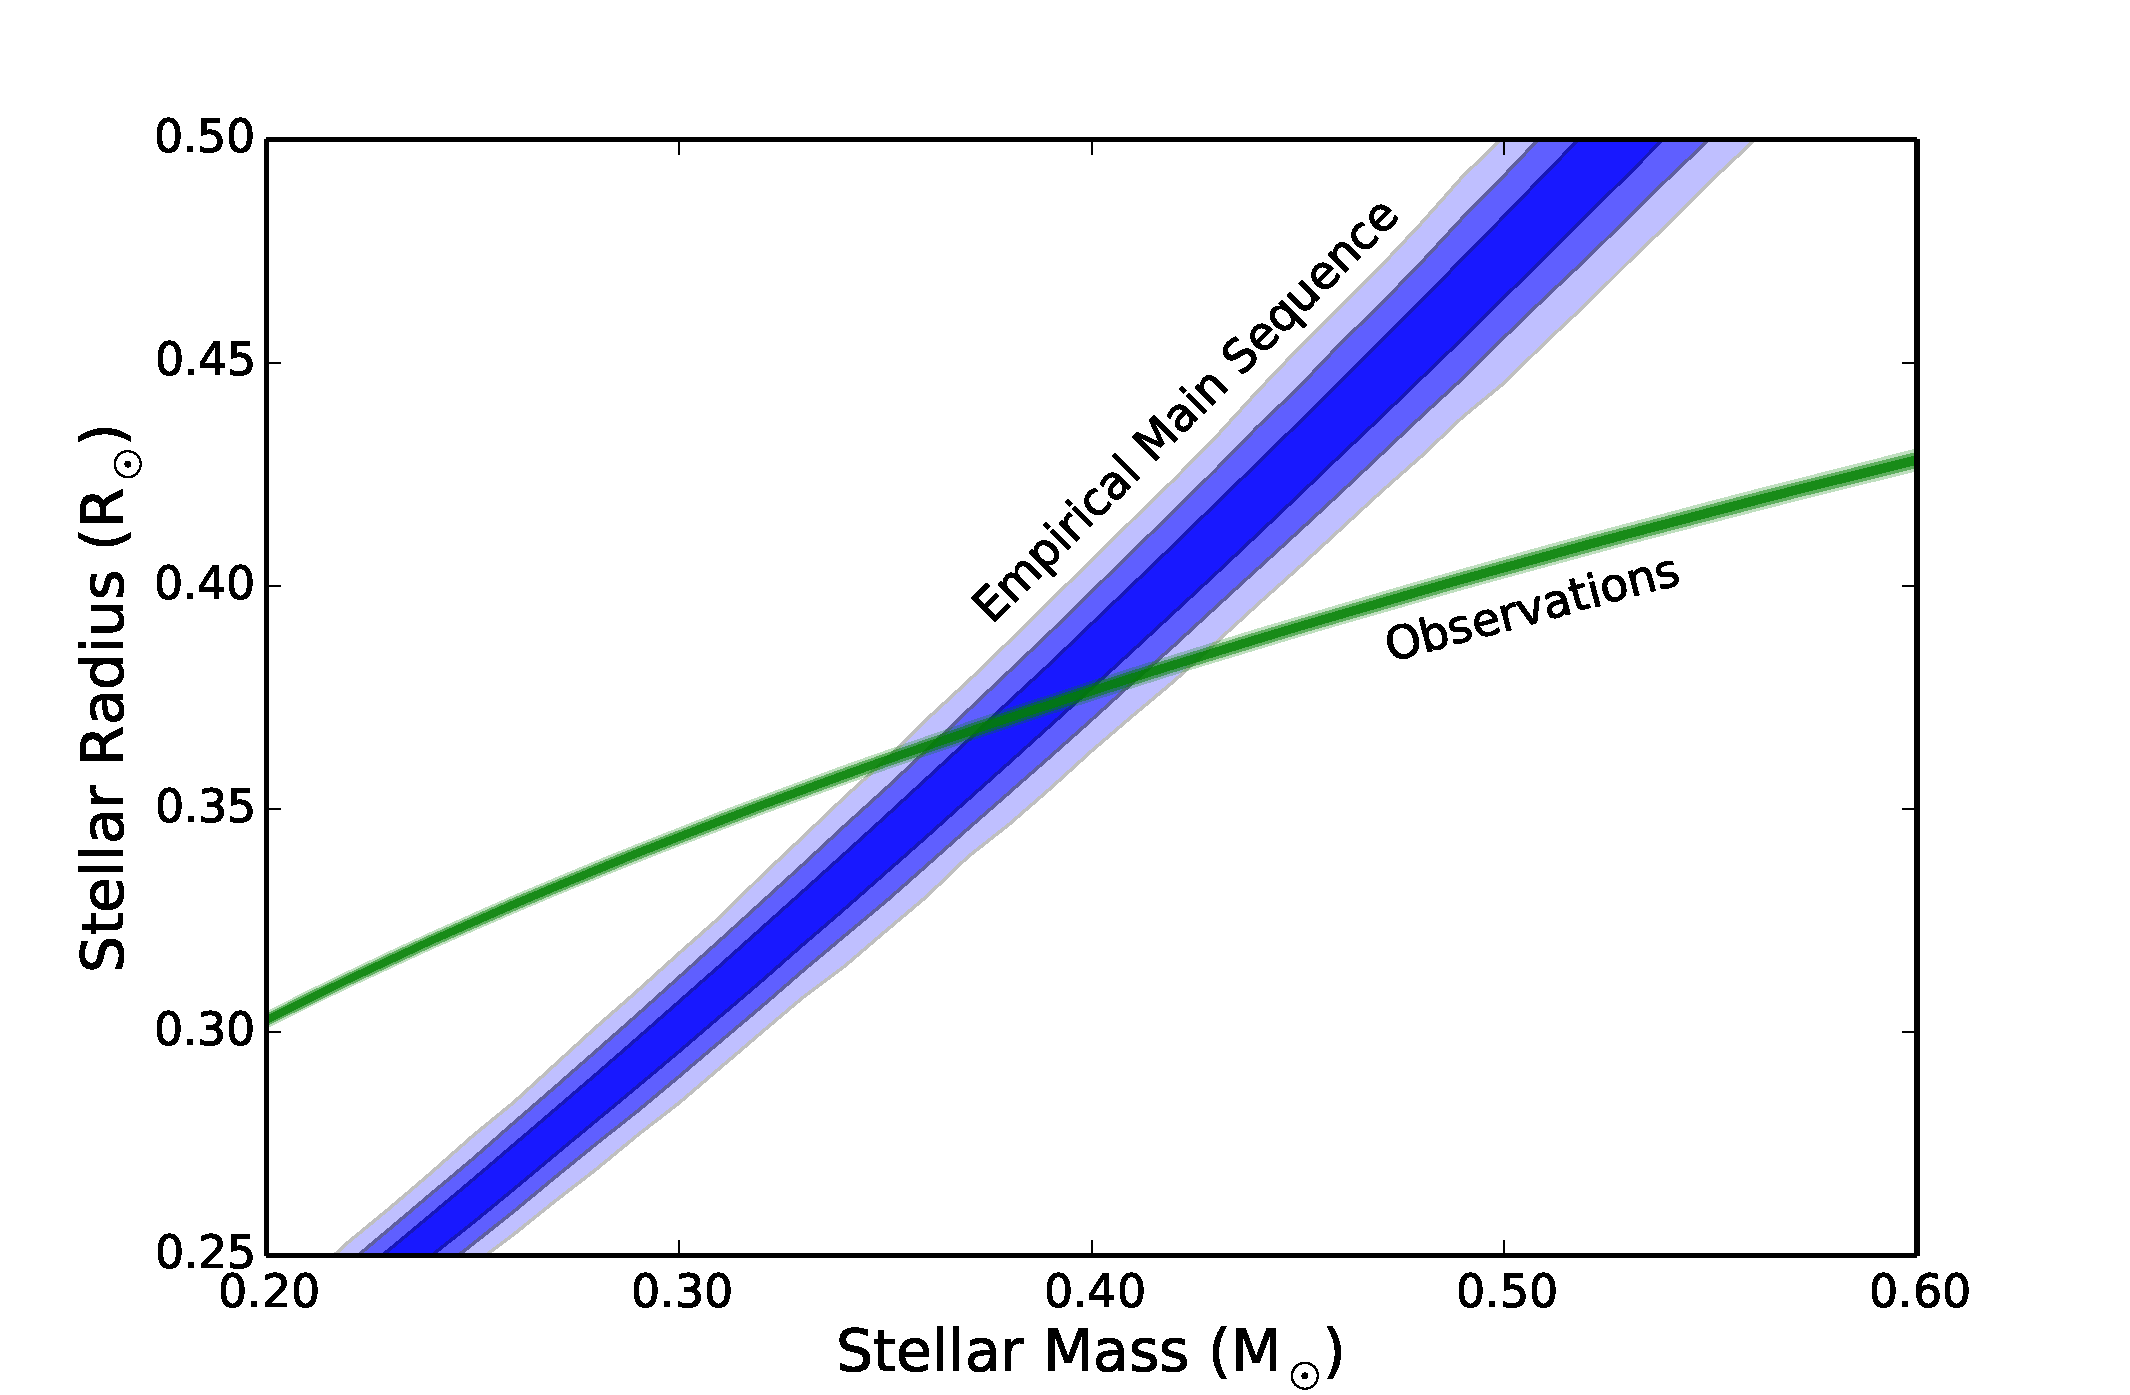
\includegraphics[width=0.75\textwidth]{chapter4/f8.pdf}}
\caption[Allowed mass-radius relation for LHS\,6343\,A from observations compared to the main-sequence]{(green) Mass-radius relation for \LA{} from the observed transit light curve and RV observations, plotted with (blue) the mass-radius relation for K and M dwarfs of \citet{Boyajian12}. There are many possible stellar masses and radii which are formally allowed, but are unphysical. By combining weak constraints from empirical observations of the main sequence, a robust direct measurement on the mass and radius of both \LA{} and \LC{} can be made.
}
\label{M-R}
\end{figure}


Because a nonzero mass ratio is required, this method is likely only applicable when the companion is a hot Jupiter, transiting brown dwarf, or low-mass stellar companion.
Moreover, it requires precise knowledge of both the Doppler semiamplitude and transit parameters. 
Therefore, the potential of this method is likely limited at present to hot transiting companions orbiting bright host stars.
Yet for these cases this technique may be very useful, especially when stellar evolutionary models may have systematic errors, such as when the host is an M dwarf or subgiant star.






\chapter{Spitzer Secondary Eclipse Observations of LHS\,6343\,C Yield Brightness Temperature and mid-T Spectral Class}

\label{chap:lhsspitz}
In this chapter I continue the discussion of LHS\,6343\,C.
Given the precise mass and radius measured in the previous chapter, we considered what observations would be necessary
to compare this object to the field brown dwarfs with well-characterized atmospheres but no direct measurements of
their masses and radii.
We concluded the best opportunity to measure the atmosphere of the brown dwarf would be through secondary eclipses
observations of the system as observed with \spitz, leading to a successful Cycle-10 proposal to observe four eclipses, 
two in each \spitz\ bandpass.
In this chapter I analyze these data and compare them to both theoretical models of brown dwarfs and empirical observations
of field brown dwarfs.
This chapter was originally published as ``Benchmark Transiting Brown Dwarf LHS\,6343\,C: Spitzer Secondary Eclipse Observations Yield Brightness Temperature and mid-T Spectral Class,'' ApJL, 822, 6 (2016) by BTM, John Johnson,
Jonathan Fortney, and Jean-Michel Desert.



\section{Introduction}
\label{sec:intro}

There are only
eleven brown dwarfs with measured 
masses and radii \citep[hereafter M15, and references therein]{Montet15a}.
These objects serve as useful benchmark stars to compare theoretical 
predictions of physical parameters for the thousands of known brown dwarfs with
measured luminosities, colors, or other atmospheric parameters 
\citep{Faherty13, Mace13, Helling14}.
Such comparisons are not currently possible as the only brown dwarfs with measured
masses and radii and inferred atmospheric parameters are larger than field objects 
due to youth or irradiation
and therefore not representative of their old, isolated counterparts 
\citep{Stassun06, Siverd12}.


Recently, M15 announced refined physical properties of the transiting
brown dwarf \LC\ \citep{Johnson11a}, measuring a mass of $62.1 \pm 1.2$ \mjup{} and a radius of 
$0.783 \pm 0.011$ \rjup. These authors also detected a secondary eclipse in the
\itk\ dataset with a depth of $25 \pm 7$ ppm.
This $3.6 \sigma$ detection is insufficient for atmospheric characterization,
but it allows for the possibility of observations at other 
wavelengths to probe the temperature, age, and atmospheric properties of the 
brown dwarf.
\LC\ presents the first opportunity to robustly measure the
atmospheric properties of an old, non-inflated brown dwarf with a known mass
and radius, enabling a key connection between the field and transiting 
brown dwarf populations.


\spitz\ \citep{Werner04} enables us to obtain observations of the secondary eclipse of
\LC\ behind \LA, providing an opportunity to measure the emitted 
near-IR radiation from the brown dwarf. 
Given the low level of irradiation from the host star, \LC\ should behave 
like a field brown dwarf for which direct mass and radius measurements 
are generally unobtainable (\textsection 5.1)

In this paper, we present detections of the secondary eclipse of \LC\ in both
 \spitz\ IRAC bandpasses.
We measure the eclipse depths by jointly fitting a Gaussian process (GP) model
to the instrumental systematics and a physical model of the astrophysical
signal.
We use these data to infer a temperature and age of the system through 
theoretical models of brown dwarf evolution, making \LC\ the first 
non-inflated brown dwarf with a known mass, radius, and direct measurement
of its atmospheric properties. 


\section{Data Collection and Analysis}


We collected data during four separate eclipses with \spitz, two 
each in the 3.6 and 4.5 $\mu$m IRAC bands \citep{Fazio04}. 
These data were collected on 2014 July 06, July 19, September 21, and October 16
as a part of \spitz\ Cycle 10 program 10122 (PI Montet).
Data in both bandpasses were collected in subarray mode with 2.0 second exposures.
In all observations, a 30-minute peak-up preceded the science observations
to place the star on the detector ``sweet-spot'' to minimize pixel-phase effects
\citep[e.g.][]{Ballard10}.
Each set of science observations contains a total of 8768 frames spread over
4.9 hours approximately centered on the time of eclipse.
For computational feasibility, we binned the observations by a factor of
eight, giving a cadence of $\approx$16 seconds per binned data point,
shorter than any astrophysical quantity of interest.

We measure the observed flux in each binned frame by performing aperture photometry,
repeating this procedure 11 times with circular apertures between 1.6 and 3.5 pixels.
By fitting a two-dimensional
Gaussian to the 5x5 region of the detector directly surrounding the brightest pixel,
we measure the position of the star on the detector in each frame \citep{Agol10}.
We find a scatter of $\sim$0.1 pixels during each observation.
A background estimate is calculated by fitting a Gaussian
to the histogram of flux values obtained over each full frame.

\subsection{Noise Model}

The \spitz\ light curves are dominated by instrumental systematics largely caused by 
intrapixel variability in the sensitivity of the InSb detector \citep{Charbonneau05, Knutson08}.
To account for these systematics, we fit an instrumental model 
simultaneously with our secondary eclipse model.
Our instrumental model is the GP model of \citet{Evans15},
who employ a covariance kernel which is a function of the centroid $xy$ coordinates of the
star and the time $t$ of the observation. 
For any two points $i$ and $j$, their covariance is defined such that
\begin{equation}
K_{ij} = k_{xy} + k_t,
\end{equation}
where
\begin{equation}
k_{xy} = A_{xy}^2 \exp\bigg[-\bigg(\frac{x_i - x_j}{L_x}\bigg)^2 - \bigg(\frac{y_i - y_j}{L_y}\bigg)^2 \bigg]
\end{equation}
and
\begin{equation}
k_t = A_t^2 \bigg[1 + \frac{t_i - t_j}{L_t} \sqrt{3} \bigg] \exp \bigg[ - \bigg(\frac{t_i - t_j}{L_t}\bigg) \sqrt{3}\bigg].
\end{equation}
Here, $x_i$ and $y_i$ are the centroid positions of the star during the $i$th observation, taken at time $t_i$. 
$A_{xy}$ and $A_t$ define the magnitude of the correlation between data points and 
$L_x$, $L_y$, and $L_t$ define the length scales of said correlation. 
A larger value of $K_{ij}$, when the temporal or spatial separation between two points is small
relative to $L_t$, $L_x$, or $L_y$, implies a stronger correlation.

Our noise model then has 19 free parameters. As each observation falls on a different region
of the detector, $A_{xy}$, $A_t$, $L_x$, and $L_y$ are not shared between observations. 
$L_t$ is shared between observations. 
We also fit for two white noise parameters, one for each bandpass, added in quadrature to our covariance kernels.

\subsection{Physical Model}

Simultaneously we fit a physical model of the secondary eclipses of \LC\ behind \LA. 
We use the transit model of \citet{Mandel02} with no limb darkening, as the primary star
is not being occulted:
the observed flux should be unchanging between second and third contact. 
We fit for four separate eclipse depths, allowing for the possibility of variability 
similar to that observed in \spitz\ surveys of field brown dwarfs \citep{Buenzli12, Metchev15}.
We also fit the orbital period, radius ratio between \LA\ and \LC, time of transit,
eccentricity vectors $\sqrt{e} \cos \omega$ and $\sqrt{e} \sin \omega$, reduced semimajor
axis $a/R_\star$, and impact parameter.
For each of these, we apply a prior following the results of the simultaneous RV and transit 
fit of M15. 
With 11 parameters defining the astrophysical model, we have 30 parameters total.
Our model is shown in Figure \ref{fig:eclipses}.


\begin{figure}[htbp!]
\centerline{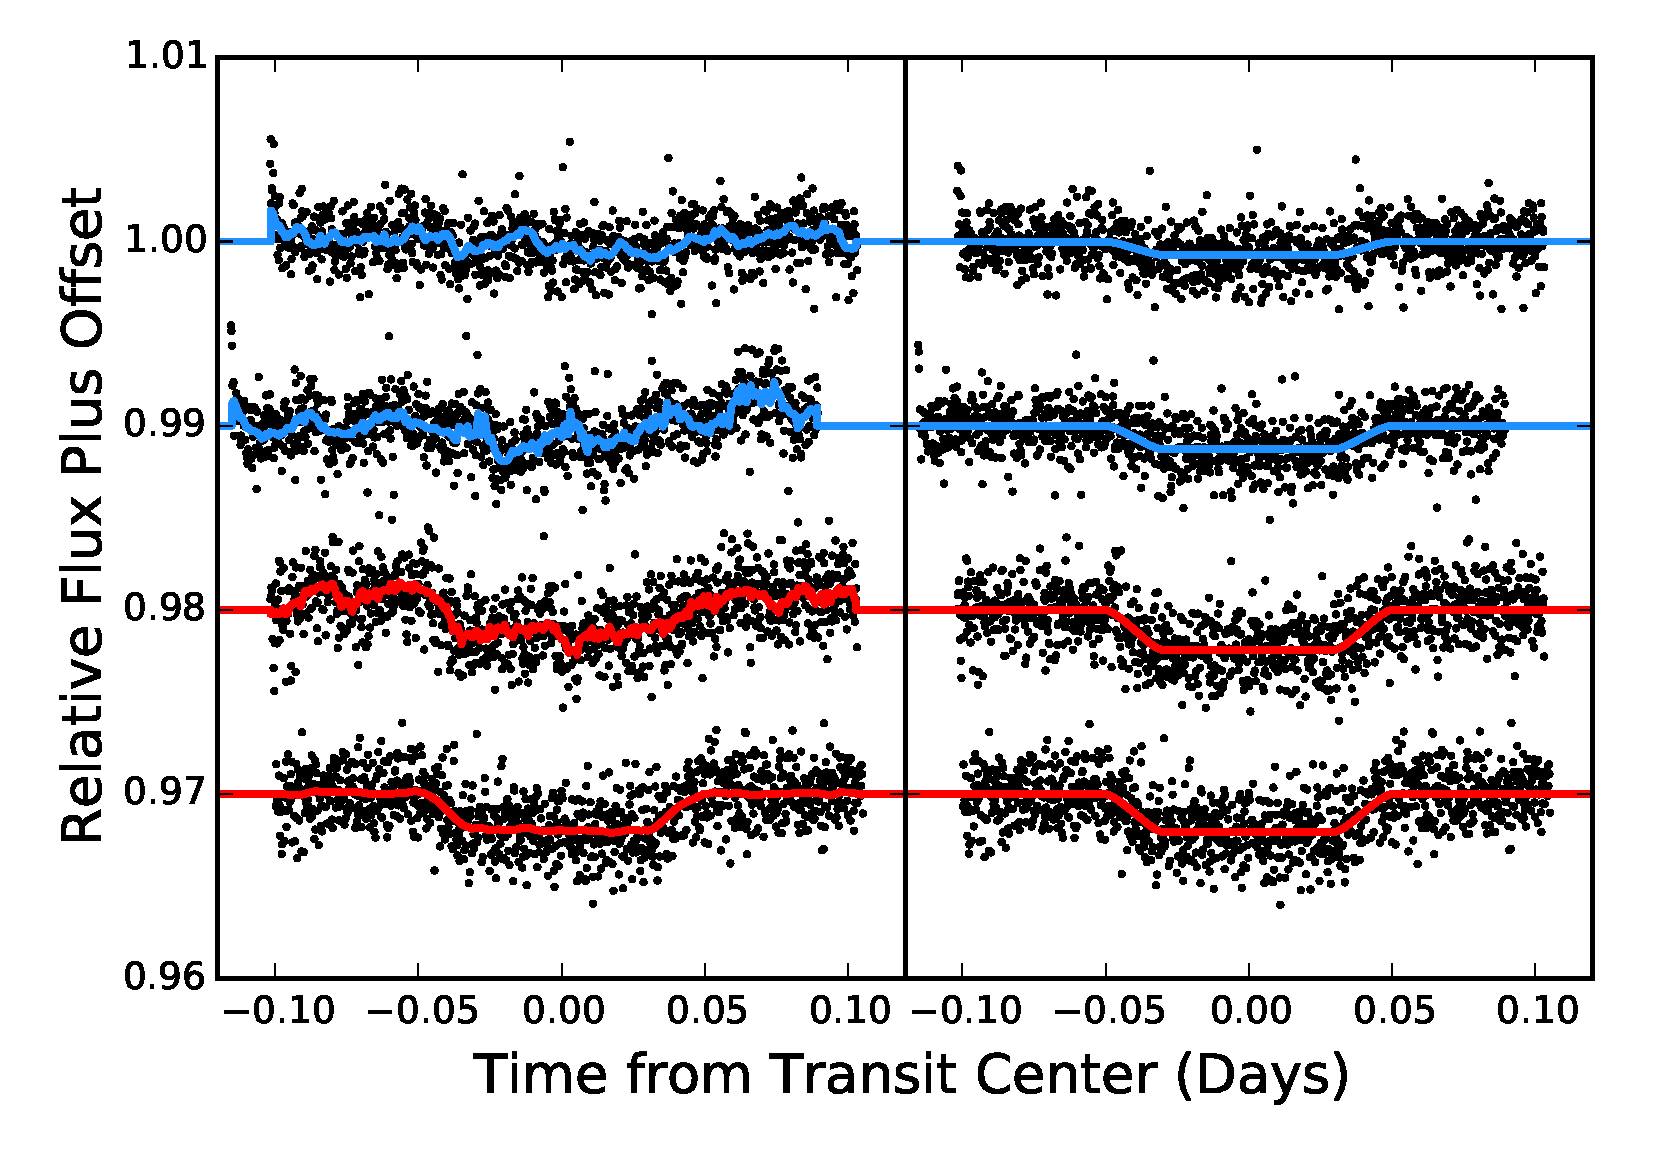
\includegraphics[width=0.75\textwidth]{chapter5/f1.pdf}}
\caption[Observed secondary eclipses of \LC, both with and without the maximum likelihood noise model removed]{(Left) Observed secondary eclipses of \LC. The solid line represents the maximum likelihood
joint fit of the instrumental and astrophysical models. The observations are arranged chronologically from
top to bottom. The top two, in blue, are eclipses in the IRAC 1 \ira\ bandpass. The bottom two,
in red, are taken in the IRAC 2 \irb\ bandpass. (Right) The same eclipses, with the maximum likelihood
instrumental model divided out for illustration.}
\label{fig:eclipses}
\end{figure}


\subsection{Parameter Estimation}
We first calculate a maximum likelihood solution for each eclipse with each of our 
eleven apertures. We then choose the single aperture which maximizes our likelihood
function and restrict ourselves to that aperture. 
For the first \ira\ eclipse and both \irb\ eclipses, we find the likelihood
function is maximized with a 2.0 pixel aperture;
for the other \ira\ eclipse, we use a 2.3 pixel aperture.
In all cases, these apertures include both M dwarfs in the system.
To compute the covariance matrix and likelihood function for each model,
we use \texttt{george}\footnote{http://dan.iel.fm/george}, 
an implementation of the hierarchically off-diagonal low-rank matrix solver of
\citet{Ambikasaran15}.


To infer the eclipse depths, we then explore the parameter space 
using \texttt{emcee} \citep{Foreman-Mackey12},
an implementation of the affine-invariant ensemble sampler of \citet{Goodman10}.
We initialize 200 walkers clustered around the maximum likelihood
values for each eclipse. 
We then allow these walkers to evolve for 1,500 steps, limiting 
each noise parameter to values within a factor of $e^{10}$ of the maximum 
likelihood value.
We remove the first 600 steps as burn-in and
verify our system has converged through the test of \citet{Geweke92} and 
visual inspection.

\section{Results}

Our results are shown in Table 1. 
We find less correlated noise in the \irb\ bandpass, in line with
previous \spitz\ analyses \citep{Hora08}.
We do not find significant evidence for variability between eclipses.
In the \ira\ bandpass the two depths are consistent at $1.4 \sigma$;
at \irb, $0.8\sigma$.
We consider these observations to represent the system in similar states
and combine the likelihoods on the eclipse depth through a kernel density
estimation of each individual depth.
From this, we measure an eclipse depth of $1.06 \pm 0.21$ parts per thousand (ppt) at \ira\ and $2.09 \pm 0.08$ ppt
at \irb, as shown in Figure \ref{fig:depths}.
We also calculate brightness temperatures for each bandpass using the BT-Settl model spectra of \citet{Allard12}
to infer the expected blackbody flux from the brown dwarf, finding $T_b = 1026 \pm 57$ K at \ira\ and $T_b = 
1249 \pm 36$ K at \irb.

\begin{table}[hbt!]
\centering
\begin{tabular}{lccc}
\hline
\footnotesize
Parameter & Median    & & Uncertainty \\
 & & & ($1\sigma$) \\
\hline
\textit{IRAC 1 Parameters}\\
Transit Depth, 2014 July 06 (ppt) & 0.74 & $\pm$ & 0.27 \\
Transit Depth, 2014 July 19 (ppt) & 1.26 & $\pm$ & 0.24 \\
Transit Depth, Combined (ppt) & 1.06 & $\pm$ & 0.21 \\
$M_A$ (Vega)$^1$ & 6.56  & $\pm$ & 0.08 \\
$M_B$ (Vega)$^1$ & 6.97 & $\pm$ & 0.10 \\
$M_C$ (Vega)& 13.43 & $\pm$ & 0.23 \\
$T_b$ (K) & 1026 & $\pm$ & 57 \\
\\
\textit{IRAC 2 Parameters}\\
Transit Depth, 2014 September 21 (ppt) & 2.16 &$\pm$  & 0.12 \\
Transit Depth, 2014 October 16 (ppt) & 2.03 & $\pm$ & 0.12 \\
Transit Depth, Combined (ppt) & 2.09 & $\pm$ & 0.08 \\
$M_A$ (Vega)$^1$ & 6.45  & $\pm$ & 0.07 \\
$M_B$ (Vega)$^1$ & 6.86 & $\pm$ & 0.09 \\
$M_C$ (Vega) & 12.58 & $\pm$ & 0.07 \\
$T_b$ (K) & 1249 & $\pm$ & 36 \\
\\
\textit{System Parameters} \\
Time of Secondary Eclipse (BJD - 2400000) & 56845.401 & $\pm$ & 0.001 \\
Orbital Period (days)$^2$ &  12.7137941 & $\pm$ & 0.0000002 \\
Eccentricity Vector $e \cos \omega$ & 0.0229 & $\pm$ & 0.0001 \\
Star C Surface Gravity (m s$^{-2}$)$^2$ & 2630 & $\pm$ & 50  \\
Star C Luminosity ($\log(L_\star /L_\odot$))$^3$  & -5.16 & $\pm$  & $0.04$  \\
Star C Temperature$^3$ (K) & 1130 & $\pm$ & 50 \\
Star C Age (Gyr)$^3$ & 5 & $\pm$ & 1 \\
\hline
\end{tabular}
\caption[Measured parameters for the LHS\,6343\,ABC system]{Measured parameters for the LHS\,6343\,ABC system. \\
(1) Inferred through $VRJHK$ photometry and the Dartmouth models of \citet{Dotter08}  \\
(2) From M15 \\
(3) Dependent on the BT-Settl evolutionary models of \citet{Allard12}}
\label{tab:results}
\end{table}

\begin{figure}[htbp!]
\centerline{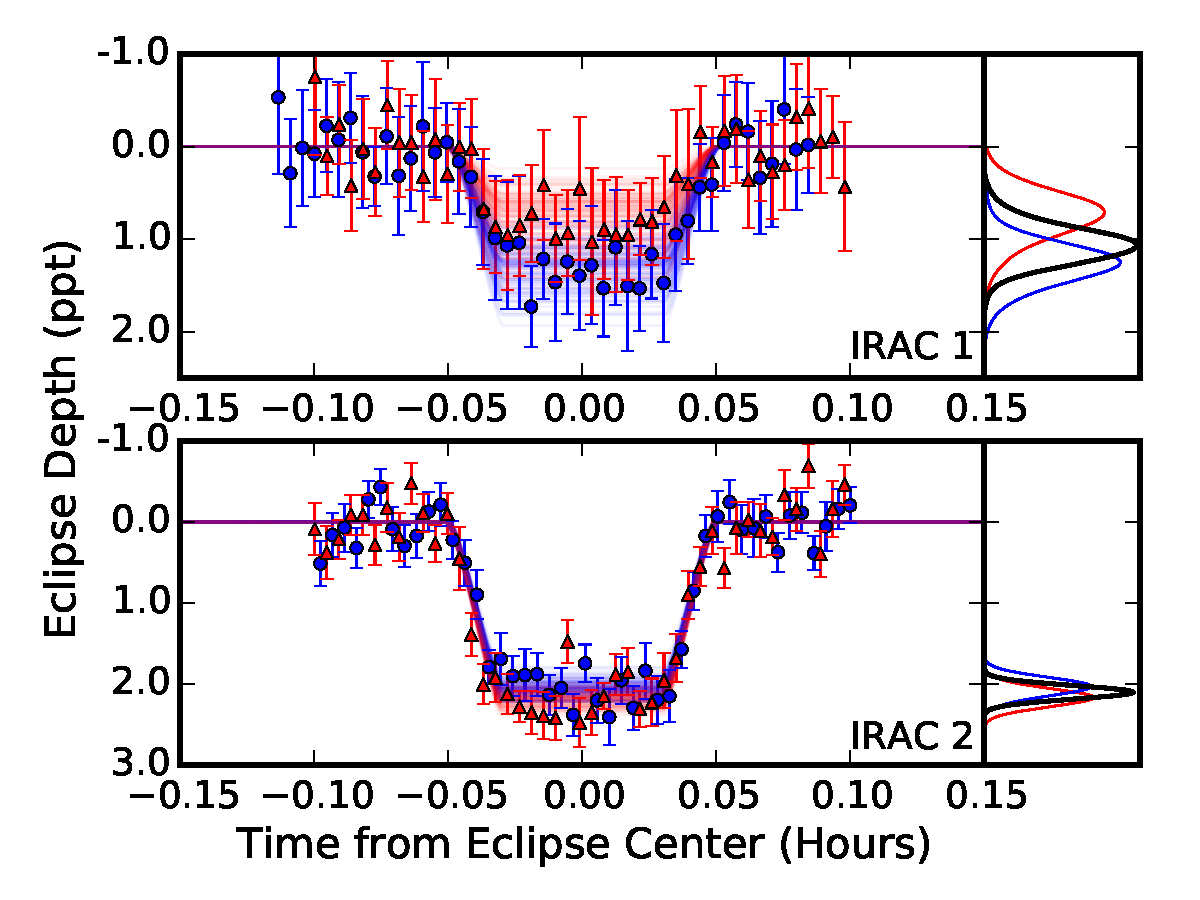
\includegraphics[width=0.75\textwidth]{chapter5/f2.pdf}}
\caption[Observed secondary eclipses and marginalized posterior distributions of the measured eclipse depths]{(Left) Observed secondary eclipses in each bandpass, with different transits in
each bandpass labeled with red triangles and blue circles. A representative instrumental
model has been removed for clarity. Red and blue lines represent 
draws from the transit model posterior distributions.
(Right) Marginalized posterior distributions of the eclipse depth for each individual
transit (red, blue) and combined (black). The observed eclipse depths are
consistent at $1.4 \sigma$ in the \ira\ IRAC 1 bandpass and 
$0.8\sigma$ in the \irb\ IRAC 2 bandpass. We find depths of
$1.06 \pm 0.21$ ppt at \ira\ and $2.09 \pm 0.08$ ppt at \irb. }
\label{fig:depths}
\end{figure}



To test the robustness of our GP model, we calculate the maximum
likelihood solutions with two different instrumental models.
Following \citet{Knutson08}, we fit a second-order polynomial
to the inferred centroid positions of the star to decorrelate the telescope motion
from the astrophysical signal. 
We also apply the pixel-level decorrelation method of \citet{Deming15}, which
decorates the observed fluxes against the pixel counts inside a subarray centered on the
PSF of the star.
In both cases, we find no statistical difference on the inferred eclipse depths.




\section{Temperature and Age of \LC}

Given the \spitz\ eclipse depths and the known mass and radius of \LC, 
we can infer the temperature of \LC\ and the age of the system. 
The eclipse depths only provide a ratio between the flux
from the brown dwarf and the two M dwarfs:
\begin{equation}
\delta = \frac{F_C}{F_A + F_B + F_C}.
\end{equation}
We have no direct measurement of the brightness of the two M dwarfs in the
IRAC bandpasses so we must infer them.
M15 use the Dartmouth stellar evolutionary models of \citet{Dotter08}
to infer a mass and radius for each star given available $VRJHK$ photometry.
Here, we use the posterior distributions on the stellar masses and the Dartmouth models to predict
the absolute magnitudes of the stars at 3.6 and \irb (Table 1).
This technique also reproduces the expected brightness of the M dwarfs to within the
photometric uncertainties in all bandpasses where we do have data.
We then use these predictions and the observed eclipse depths to 
calculate the absolute magnitude of \LC\ in 
both IRAC bandpasses: we determine $M_{C, 3.6} = 13.43 \pm 0.23$ and 
$M_{C, 4.5} = 12.58 \pm 0.07$ so that $[3.6 - 4.5] = 0.85 \pm 0.24$.
We repeat this procedure with the resolved flux measurements and the BT-Settl
evolutionary models of \citet{Allard12}, finding no difference in the 
extrapolated IRAC absolute magnitudes of the M dwarfs at the $1\sigma$ level.


Brown dwarf evolutionary models can be used to determine a temperature
and age of \LC.
We investigate the predictions of several models.



\begin{figure}[htbp!]
\centerline{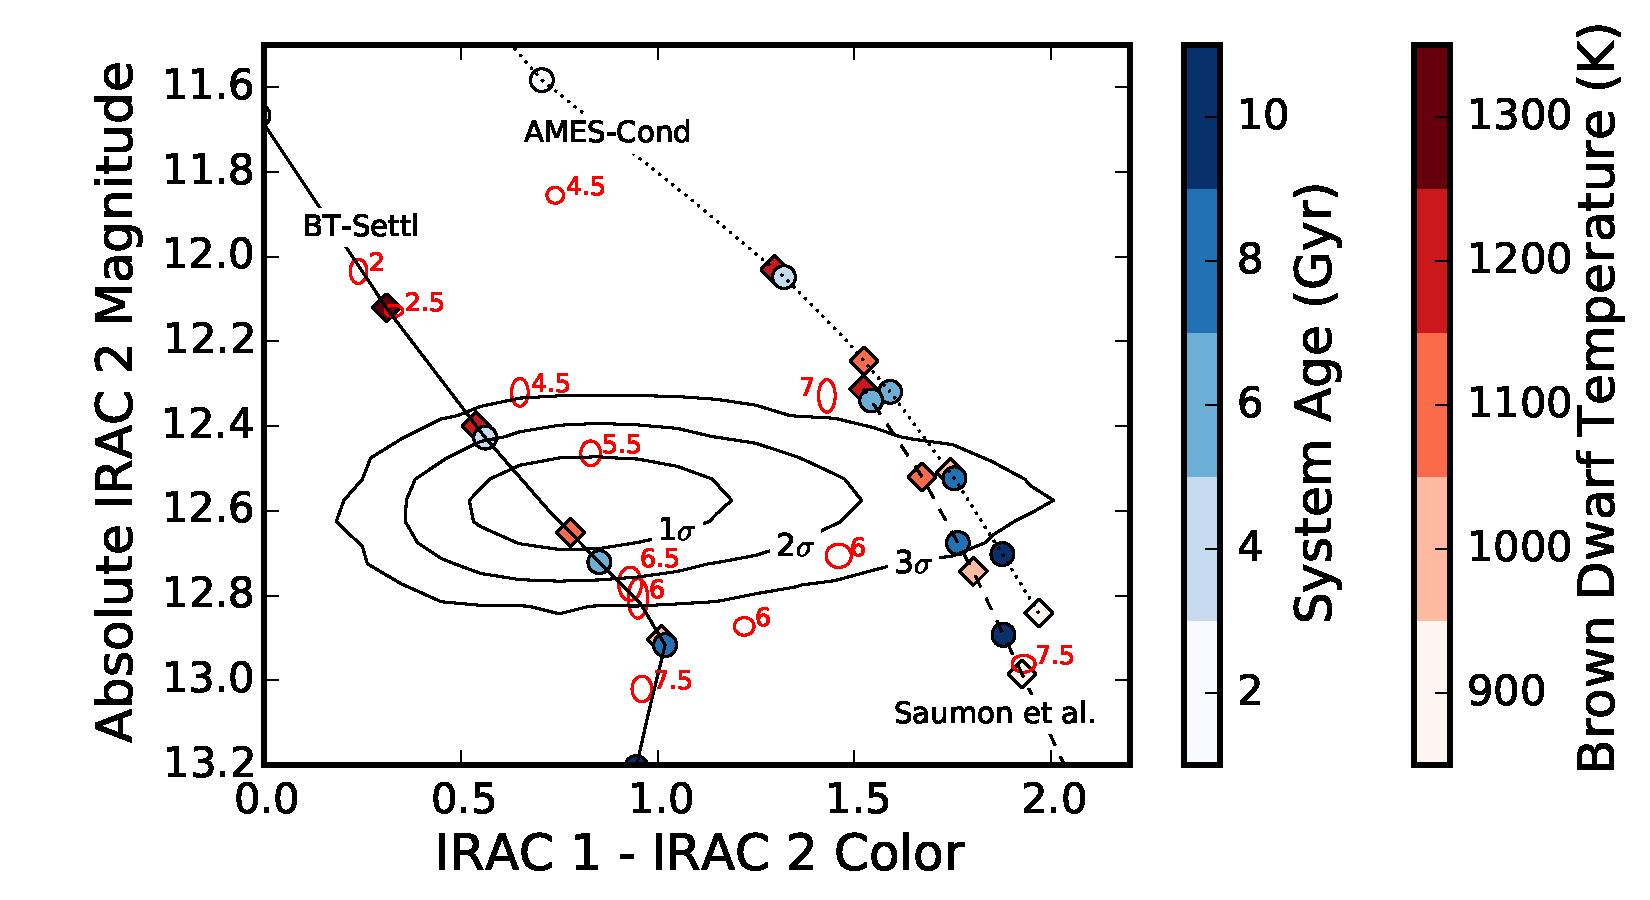
\includegraphics[width=0.75\textwidth]{chapter5/f3.pdf}}
\caption[Color-magnitude diagram showing the absolute magnitude in the IRAC 2 \irb\ bandpass
against the IRAC 1 - IRAC 2 color]{Color-magnitude diagram showing the absolute magnitude in the IRAC 2 \irb\ bandpass
against the IRAC 1 - IRAC 2 color. Contours represent the allowed parameter space in which \LC\ could 
reside. The labeled lines represent the theoretical evolutionary tracks of a brown dwarf with the mass of 
\LC\ from (left to right) the BT-Settl, \citet{Saumon12}, and AMES-Cond models. Dots correspond to model predictions
at (white to dark blue) 2, 4, 6, 8, and 10 Gyr; diamonds correspond to model predictions for temperatures of
(white to dark red) 900, 1000, 1100, 1200, and 1300 K.The BT-Settl model provides a good fit at $5 \pm 1$ Gyr; the 
AMES-Cond and Saumon models fit the data at lower significance at $8 \pm 1$ Gyr. 
Red ellipses represent field brown dwarfs from \citet{Dupuy12} and \citet{Filippazzo15}; labels represent the spectral subtype inside the T class.  }
\label{fig:CMD}
\end{figure}

The BT-Settl models provide the best fit to the available data. We use the isochrones
calculated for the CIFIST 2011 abundances and opacities \citep{Caffau10, Allard12}, the most recent for which 
magnitudes have been tabulated at these masses and ages.
With this model grid, we infer a brown dwarf with $t = 5 \pm 1$ Gyr, $T = 1130 \pm 50$ K,
and $\log(L_\star /L_\odot = -5.16  \pm   0.04$ by evaluating the likelihood of the model fit to our calculated absolute magnitudes
in each bandpass and marginalizing over all other parameters. 
This strategy provides an estimate of the statistical error, but not the systematic error caused by uncertainty
or errors in the models.
We note that of field brown dwarfs with measured temperatures
and colors, this model set predicts the correct temperatures with a scatter of $\sim 50$K, consistent with 
the published uncertainties in temperature.

The AMES-Cond models of \citet{Allard01} provide a fit to the \spitz\ photometry,
mass, and radius of \LC\ such that $t = 8 \pm 1$~Gyr and $T = 1000 \pm 50$~K.
However, this model grid underpredicts the \ira\ luminosity, leading to an overestimation
of the [3.6 - 4.5] color at all ages (Figure \ref{fig:CMD}).
The AMES-Dusty models, meanwhile, do not provide a good fit, overpredicting the luminosity
even if the system were the age of the universe, as is common with brown dwarf models
\citep{Rice10, Dupuy15}.

The isochrones of \citet{Saumon08} combined with synthetic photometry from \citet{Saumon12} 
predict IRAC photometry as a function of temperature and system age.
These models provide a slightly better fit to the data than the AMES-Cond
models for an $1100 \pm 50$ K brown dwarf, but still overpredict the [3.6 - 4.5] color.
Their hybrid models, meant to model the L/T transition, suggest an older brown dwarf with an age
of $8 \pm 1$ Gyr.
Their cloudy L dwarf models do not provide a good fit at any age.
Given the inability of the cloudy models to explain the observations, as well as the consistency 
between models in predicting temperatures below the L/T transition
\citep{Burgasser02, Golimowski04}, we confirm \LC\ as a T dwarf.


Objects near the L/T transition with temperatures 1000-1400 K
are particularly challenging for brown dwarf evolutionary models.
The uncertainties in all models are dominated by systematics, so we
cannot develop one statistical posterior on the 
temperature or age. 
We note the BT-Settl models provide the best fit to these data and to the population of similar mid-T dwarfs in color-magnitude
space.
This system compares favorably to other known T5-6 dwarfs \citep[Figure 3]{Dupuy12}. Of the field brown dwarfs with measured luminosities and temperatures, it is consistent
with being between T4.5 dwarf 2MASS\,0000+2554 ($1227 \pm 95$ K) and T6 dwarfs 2MASS\,0243-2453 ($973 \pm 83$ K) and 2MASS\,1346-0031 \citep[$1011 \pm 86$ K,][]{Filippazzo15} in its evolution.
This age measurement, while model dependent, is the first measurement of the age of the system: previously, 
\citet{Johnson11a} were able to only place a lower limit of 1-2 Gyr on the system age.


\section{Discussion}

\subsection{Irradiation from \LA}

We ignore irradiation from \LA.
Given the (Dartmouth model-dependent) temperature of the host of $3430 \pm 20$ K 
and semi major axis $a/R_\star = 46.0 \pm 0.4$, the equilibrium temperature
of the brown dwarf is $T_{eq} = 365\pm 3$ K, assuming a Bond albedo of 0.07, expected for 
a massive brown dwarf around an M2V dwarf \citep{Marley99}.
Therefore, the emitted flux as a result of the absorption and reemission of stellar 
radiation from \LA\ is $\approx 1\%$ the total flux. 
While irradiation may affect the thermal profile of the brown dwarf, it should
be negligible considering the $\approx 0.1$~mag uncertainties on the brown dwarf's 
magnitude.

Moreover, given the advanced age of the system, we expect high energy 
irradiation from the host star to be negligible. \citet{West08} find a rapid decay
in M dwarf magnetic activity over stellar age; \citet{Shkolnik14}
find the same to be true for UV emission, with a steep drop in UV emission at ages
above $1$ Gyr.
\citet{Stelzer13} study nearby M dwarfs to find X-ray emission decays even more quickly
for M dwarfs than UV emission, with a difference of three orders of magnitude between 
young M dwarfs in TW Hydra and old, field M dwarfs.
Any high energy radiation that may have once influenced the atmosphere of \LC\ has 
been at a low level for billions of years, allowing the brown dwarf to 
achieve an equilibrium representative of field brown dwarfs.

\subsection{Metallicity of \LC}

M15 infer a metallicity for the two M dwarfs in the system 
$[\textrm{a/H}] = 0.02 \pm 0.19$.
If the brown dwarf formed through core accretion, it may be expected to have
a higher metallicity than its host stars \citep{Pollack86, Podolak88},
as is the case for the planet orbiting GJ\,504 \citep{Skemer15}. 
Because of the low mass of the host star and likely low mass of its protoplanetary disk
\citep{Andrews13}, it is considerably more likely this brown dwarf formed like a binary
star system so that the metallicity of \LC\ is likely not significantly different from its
host star \citep{Desidera04}.
Additional observations that infer a spectrum of \LC\ can provide 
tests of theoretical brown dwarf spectra given the known metallicity of the system.
These tests are especially important for mid/late T dwarfs, where metallicity effects
can affect near-IR colors by as much as 0.3 dex \citep{Burningham13}.



\subsection{Dynamical History of \LHS}

The secondary eclipses are centered at phase $0.5146 \pm 0.0001$, corresponding
to times of transit $0.185 \pm 0.001$ days after half-phase between
successive primary transits, or an eccentricity vector 
$e \cos{\omega} = 0.0229 \pm 0.0001$.
This value is consistent with that inferred from RV observations and 
\itk\ photometry ($0.0228 \pm 0.0008$, M15)


The eccentricity in the \LA-C subsystem may be primordial or the result
of dynamical perturbations from star B. 
\LB\ is presently at a sky-projected separation of $\sim$20 AU from the A-C subsystem.
Depending on the orbit of \LB, the system may be susceptible to Kozai-Lidov oscillations
\citep{Kozai62, Lidov62}.
Kozai-Lidov cycles would lead to oscillations in the orbital inclination and eccentricity 
of the A-C subsystem on a timescale
\begin{equation}
\tau \approx P_C \frac{M_{AC}}{M_B} \bigg(\frac{a_{AC-B}}{a_{AC}}\bigg)^3 (1 - e_{AC-B})^{3/2},
\end{equation}
where $P_C$ is the orbital period of the brown dwarf, $M_{AC}$ the A-C subsystem mass,
$M_B$ the perturber mass, $a_{AC-B}$ and $e_{AC-B}$ the orbital semimajor axis and 
eccentricity of star B around the AC subsystem, and $a_{AC}$ the orbital semimajor axis
of C around A.
The two M dwarfs have similar masses. The semimajor axis $a_{AC} = 0.08$ AU is known,
but we only know the instantaneous sky-projected separation between AC and B is $\approx $20 AU.
Taking this value as a proxy for the true semimajor axis, we find
$\tau \sim 10^6 (1-e_{AC-B})^{3/2}$ years. Even for significantly larger orbits of star B and 
high eccentricities, the timescales for Kozai-Lidov cycles would be shorter
than the $\sim 10^{10}$ year age of the system, suggesting the system may be susceptible
to Kozai-Lidov oscillations given appropriate initial conditions.

The current orbit can provide clues about the dynamical history of this system. 
Measurement of an inclined orbit of \LB\ through astrometric 
monitoring could provide evidence for Kozai-Lidov cycles, as would a 
misalignment between the spin axis of \LA\ and the orbit of \LC.
While close binaries are not always neatly aligned \citep{Albrecht14},
they often are, especially for low-mass binaries \citep{Harding13, Triaud13}.










\chapter{Masses and Orbital Parameters of GJ\,3305\,AB, the Wide Binary Companion to the Imaged Exoplanet Host 51\,Eri}
\label{chap:Mbinaries}

In this chapter I continue comparing observations of low-mass stars to predictions from theoretical models.
Throughout my graduate studies I have led a long-term program to measure masses of M dwarfs in young moving groups
through astrometric and RV observations of their orbits using the Differential Speckle Survey Instrument (DSSI) at the 
Discovery Channel Telescope and Gemini Observatory and the Tillinghast Reflector Echelle Spectrograph at 
Mt. Hopkins.
As we must observe a substantial fraction of the orbit before we can determine a unique mass, this is a long-term project
not intended to be completed during this thesis.
As a part of this thesis, we published the first results from this survey, outlining our methods and presenting the first binary
system with a closed orbit, the GJ\,3305\,AB binary.
This chapter was originally published as ``Dynamical Masses of Young M Dwarfs: Masses and Orbital Parameters of GJ 3305 AB, the Wide Binary Companion to the Imaged Exoplanet Host 51 Eri,'' ApJL, 813, 11 (2015) by BTM, Brendan Bowler, 
Evgenya Shkolnik, Katherine Deck, Ji Wang, Elliott Horch, Michael Liu, Lynne Hillenbrand, Adam Kraus, and Dave 
Charbonneau.


\section{Introduction}
\label{sec:intro}

Loose associations
of young, nearby ($<$70 pc) stars with common ages,
kinematics, and origins have been a subject of increasing interest
\citep{Zuckerman04, Shkolnik12, Malo13}.
Because of their proximity to Earth, these young
moving groups (YMGs) are excellent targets to study pre-main sequence (PMS)
stellar and substellar evolution, protoplanetary and debris disk structure,
and giant planet formation at ages between distant
star-forming regions and old field stars \citep[e.g.][]{Close05, Nielsen10}. 
About 10 YMGs containing hundreds of objects between 8 and 120 million years old 
are known \citep[e.g.][]{Torres08}.

As these moving groups are amenable to numerous age dating methods, including kinematic techniques, 
they provide the opportunity 
to measure dynamical masses of PMS low-mass binary 
objects and test stellar evolution models \citep{Stassun14}.
Generally, PMS stellar
masses are inferred by comparing a star's temperature,
luminosity and metallicity to model predictions
\citep[e.g.][]{Schaefer14}. 
These models
are poorly constrained by observations and may induce systematic
offsets \citep{Dupuy09, Dupuy14}. 
Worse yet, different models predict disparate masses, primarily
due to uncertainties in the treatment of convection in
low-gravity atmospheres \citep{Baraffe02}, stellar
accretion history \citep{Baraffe10}, and molecular line lists
\citep{Baraffe15}.
In some cases, model-predicted masses can differ by a factor of two or
more \citep{Hillenbrand04, Schlieder14}. 
Dynamical mass measurements of binary stars with known ages 
are essential to test models. 


Recently, \citet{Macintosh15} presented 51\,Eri\,b, the first
exoplanet discovery from the Gemini Planet Imager.
The planet has a mass of $\approx 2$ \mjup\ (assuming a hot start model), 
a projected separation of 13 AU,
a temperature of 600-750 K, and a T4.5-T6 spectral type.
\thisstarsix\ is known to be a binary with combined spectral type M0 
\citep{Kasper07}.
\citet{Feigelson06} identified \thisstarsix\ and 51\,Eri as an F0-M0 common proper motion pair, 
separated by $66$ arcsec or $\sim$2000 AU.

As a binary system,
a dynamical mass can be measured for both stars in \thisstarsix\,AB. 
As both stars are members of the $\beta$ Pictoris moving group, an approximate age of
the system is known \citep[$24 \pm 3$ Myr;][]{Binks14, Mamajek14, Bell15}.
While most dynamical masses of M dwarfs are limited by distance uncertainties, 
51\,Eri has a parallax from \textit{Hipparcos} measured
to a precision of 1\%.
Combining this parallax with 15 years of imaging and RV data enables us to determine
the system orbital parameters, elucidating
the architecture of this 4---or more---body system.

In this paper, we combine RV and astrometric observations of \thisstarsix\,AB 
to measure orbital parameters and masses for each star. 
We compare these masses to model predictions and
discuss the possible implications of this binary pair on the long-term evolution of
the orbit of 51\,Eri\,b.


\section{Data Collection and Reduction}
\label{sec:data}

\thisstarsix\,AB has been imaged and resolved many times
\citep{Kasper07, Bergfors10, Delorme12, Janson12, Janson14a}. 
The system was also imaged with NIRC2 \citep{Wizinowich00} in one unpublished epoch
in 2001 available in the Keck Observatory Archives (KOA, PI Zuckerman). 
In this work, we combine these data with five observations from 2002 to 2015, three
using Keck/NIRC2 and one with the Differential Speckle Survey Instrument \citep[DSSI,][]{Horch09} at 
the Discovery Channel Telescope at Lowell Observatory.

All NIRC2 data were obtained with the narrow camera mode, which has a field of view 
of 10.2 arcsec $\times$ 10.2 arcsec and a plate scale of 9.952~mas pixel$^{-1}$
\citep{Yelda10}.  All images were flat fielded and cleaned of bad pixels and 
cosmic rays.  Astrometry and relative photometry of \thisstarsix\ was derived by 
simultaneously fitting three bivariate Gaussians to each component following 
\citet{Liu10}. 

DSSI allows for simultaneous observations in two filters.
We use the DSSI $R$ and $I$ filters, with central wavelengths
692 and 880~nm and FWHMs of 40 and 50~nm. 
We obtained 1000 40-ms exposures in each channel simultaneously.
The data were then reduced following \citet{Horch15}.
Specifically, the autocorrelation of each frame was calculated and summed over all
exposures, and the near-axis subplanes of the image bispectrum were 
calculated. 
To create a reconstructed image, the Fourier transform of the autocorrelation
of the binary was divided by that of a nearby point source (HR\,1415).
The square root of this value is taken, and the result combined with a phase function
derived from the bispectral subplanes.
The pixel scale (19~mas pixel$^{-1}$ in $R$ and 20~mas pixel$^{-1}$ in $I$) and orientation of the detector were found by observing
several widely separated binaries with known astrometry.
Our astrometry is listed in Table~\ref{tab:astrometry}.

\begin{landscape}
\begin{table}[hbt!]
\scriptsize
\begin{center}
\begin{tabular}{lcccccc}
\hline
Epoch & Bandpass & RV & Contrast & Separation & Position Angle & Source \\
(Year) &   & (km s$^{-1}$) &  ($\Delta$ mag) & (mas) & (deg) & \\
\hline
2001.910 & H$_2$($\nu$=1--0) & & $1.00 \pm 0.02$ & $286  \pm 1$   & $198.1 \pm 0.1$   & This Work \\
2002.162 & $H$               & & $1.02 \pm 0.02$ & $275.4\pm 1.5$ & $197.9 \pm 0.2$   & This Work \\
2003.05  & $K$              &  & $0.94 \pm 0.05$ & $225  \pm 5^{1}$   & $195.0 \pm 1.5^{1}$   & \citet{Kasper07} \\
2003.195 & $H$              &  & $0.99 \pm 0.01$ & $217  \pm 1$   & $196.8 \pm 0.1$   & This Work \\
2004.02  & $L'$              & & & $159  \pm 2$   & $194   \pm 1$     & \citet{Delorme12} \\
2004.95  & $L'$              & & $0.88 \pm 0.28$ & $93   \pm 2$   & $189.5 \pm 0.4$   & \citet{Kasper07} \\
2008.88  & SDSS $z'$       &   & $1.39\pm 0.16$ & $218  \pm 2$   & $20.3  \pm 0.3$   & \citet{Bergfors10} \\
2008.88  & SDSS $i'$        &  & $2.57\pm 0.05$ & $218  \pm 2$   & $20.3  \pm 0.3$   & \citet{Bergfors10} \\
2009.13  & SDSS $i'$+$z'$    & &                & $231  \pm 2$   & $19.2  \pm 0.3$   & \citet{Janson12} \\
2009.90  &  $L'$             &   &              & $269  \pm 3$   & $18.6  \pm 1.0$   & \citet{Delorme12} \\
2009.98  &  $L'$             &    &             & $272  \pm 3$   & $19.2  \pm 1.0$   & \citet{Delorme12} \\
2010.10  & SDSS $z'$       &   & $1.34\pm 0.01$ & $284  \pm 3$   & $18.5  \pm 0.6$   & \citet{Janson12} \\
2010.10  & SDSS $i'$       &   & $3.73\pm 0.01$ &                &                   & \citet{Janson12} \\
2010.81  & SDSS $z'$       &   &                & $297  \pm 3$   & $19.4  \pm 0.3$   & \citet{Janson14a} \\
2011.67  &  $L'$             &    &             & $303  \pm 3$   & $18.1  \pm 1.0$   & \citet{Delorme12} \\
2011.87  & SDSS $z'$        &  &                 & $295  \pm 4$   & $18.5  \pm 0.3$   & \citet{Janson14a} \\
2012.01  & SDSS $z'$        &  &                 & $307  \pm 3$   & $18.2  \pm 0.3$   & \citet{Janson14a} \\
2014.629 & Br$\gamma$    &     & $0.92 \pm 0.01$ & $244  \pm 1$   & $16.8 \pm 0.1$    & This Work \\
2014.746 & DSSI $R$       &    & $1.89 \pm 0.04$ & $239\pm 1$ & $16.4 \pm 0.2$  & This Work \\
2014.746 & DSSI $I$        &   & $1.17 \pm 0.03$ &    $240 \pm 1$       &     $16.1 \pm 0.2$           & This Work\\
2015.653 & $K$               &    &  $0.93 \pm 0.01$ &    $199 \pm 1$      &   $15.6 \pm 0.1$     & This Work \\
2015.653 & $H$               &    &  $0.99 \pm 0.01$ &   $198 \pm 1$    &  $15.6 \pm 0.1$        & This Work \\
2015.653 & $J$               &    &  $0.97 \pm 0.01$ &    $199 \pm 1$   &  $15.6 \pm 0.2$      & This Work \\
2015.653 & $Y$               &    &  $1.06 \pm 0.03$ &   $200 \pm 1$    &  $15.6 \pm 0.1$      & This Work \\
\hline
2003.796   & HIRES $V$   & $ 19.41 \pm 0.38 $ &        &         &          & This work \\
2004.884 & NIRSPEC $K$ &  $19.86 \pm 0.05$         &        &       &         &  \citet{Bailey12} \\
2005.862 & NIRSPEC $K$ &  $20.55 \pm 0.06$         &        &       &         &  \citet{Bailey12} \\
2005.971 & HIRES $V$ &      $21.70 \pm 0.30$     &        &       &         &  \citet{Shkolnik12} \\
2006.014 & NIRSPEC $K$ &  $20.82 \pm 0.05$         &        &       &         &  \citet{Bailey12} \\
2006.016 & NIRSPEC $K$ &  $20.95 \pm 0.05$         &        &       &         &  \citet{Bailey12} \\
2006.019 & NIRSPEC $K$ &  $20.95 \pm 0.05$         &        &       &         &  \citet{Bailey12} \\
2011.778 & UVES Blue &        $24.40 \pm 0.04$   &        &       &         &  \citet{Elliott14} \\
2001.994 & UVES Blue &        $23.30 \pm 0.02$   &        &       &         &  \citet{Elliott14} \\
2012.022 & UVES Blue &        $23.80 \pm 0.02$   &        &       &         &  \citet{Elliott14} \\
\hline
\end{tabular}
\caption[Data for \thisstarsix\,AB]{Data for \thisstarsix\,AB. In some previous analyses, contrast ratios were not listed for specific epochs.
Observations without listed separations correspond to simultaneous multiband photometry. \\
(1) Observations published without uncertainty estimates; we choose conservative
values.}
\end{center}
\label{tab:astrometry}
\end{table}
\end{landscape}
\clearpage



The \thisstarsix\ binary system has also been monitored spectroscopically with a 12-year observational baseline.
One Keck/HIRES spectrum from 2003 exists in the KOA (PI Zuckerman); we measure
the RV following \citet{Kraus15}.
We combine this spectrum with nine additional spectra from \citet{Bailey12}, \citet{Shkolnik12},
and \citet{Elliott14}.
In all cases, the RVs were calculated treating the system as an SB1.
We take the reported RV and uncertainty for each observation, but assume the flux from the secondary
is non-negligible, as explained in Section~\ref{sec:analysis}.

\section{Analysis}
\label{sec:analysis}



We infer the orbital parameters of \thisstarsix\,AB by comparing the astrometric
and RV data to a Keplerian orbit model at each of the observation
times.
A parallax, astrometric orbit, and SB1 RV data can be combined to measure individual
masses of each star \citep[e.g.][]{Bean07}.
There is no measured parallax for \thisstarsix, so we adopt the Hipparcos distance to 51\,Eri/HIP\,21547: 
$29.43 \pm 0.30$ pc \citep{vanLeeuwen07}.
These two comoving systems have a projected separation of $1940 \pm 20$ AU,
or 0.01 pc. It is unlikely that the radial distance between the two could
be significantly larger while remaining bound; we apply this parallax
as a prior on the distance to \thisstarsix.

We then fit for nine additional parameters that define the orbits of
the two stars as viewed from Earth.
Of these, seven can be obtained from astrometry.
These parameters are the eccentricity vectors $\sqrt{e} \cos{\omega}$ and
$\sqrt{e} \sin{\omega}$, the time of periapse $t_P$, the period $P$, 
the total mass $M_1 + M_2$, the inclination $i$, and the 
longitude of the ascending node $\Omega$.
We parameterize the eccentricity vector in this manner following \citet{Eastman13}.
The RV data can provide additional information about several of these
(not $M_1 + M_2$ or $\Omega$ directly), also allowing us to fit the
systemic RV $\gamma$ and the secondary mass $M_2$.


We include ten additional terms to account for 
possible systematics in the datas. 
This star has been imaged, resolved, and published by four different groups.
We account for the possibility each group may have underestimated 
their uncertainties on the orbital separation and position angle
by a multiplicative factor by including a systematic error term on the measured positions 
from each group, allowing outlier points to be downweighted without manually choosing
specific points to downweight.
We do the same with our reductions of both archival and new data,
allowing for separate systematic error terms on our data from Keck/NIRC2 and 
DCT/DSSI, providing a total of six systematic error terms.
We allow the uncertainties on each dataset to be inflated up
to a factor of five.

Similarly, we allow for the possibility that the uncertainties in the 
RVs may be underestimated, possibly due to stellar variability \citep{Moulds13},
errors in systemic RVs of standard stars, or drifts in the stability of the
spectrographs.
As our RV data originate from four sources, we allow each to have its own 
systematic error term, analogous to the jitter term commonly applied 
in RV orbit fits of exoplanets \citep[e.g.][]{Johnson11b}:
\begin{equation}
\log \mathcal L \propto - \sum_i \bigg[\log{\sqrt{\sigma_{o,i}^2 + \sigma_s^2}} + 0.5 \bigg(\frac{(f_i(t) -
v_i(t))^2}{\sigma_{o,i}^2 + \sigma_s^2}\bigg)\bigg].
\end{equation}
Here, $\mathcal L$ is the likelihood of the data given some underlying physical model,
$\sigma_{o,i}$ is the observed uncertainty on the $i$th data point, $\sigma_s$ 
the systematic error associated with each particular set of observations, $f_i(t)$ the RV
model evaluated at time $t$, and $v_i(t)$ the observed RV at each $t$. 
Maximum likelihood jitter values range from $0.13$ km s$^{-1}$ for the 2003 HIRES data
to $0.57$ km s$^{-1}$ for the UVES data, suggesting stellar jitter is significant
in the RV data, as expected for young stars. 

In all cases, one set of lines are observed because the RV separation is smaller than
the line width.
We expect each RV measurement to be the flux-weighted sum of the two individual
RVs.
At each step, we calculate the RVs for each star, weighting them according to their 
expected flux contribution in each bandpass, using the observed flux ratios in the
visible and near-IR as priors and assuming an additional 0.1~mag of variability in 
the optical and 0.05~mag in the near-IR.

We neglect the possibility that 51\,Eri could contribute significantly to the observed RV signal. 
Following Equation~1 of \citet{Montet15a}, 
the maximum RV acceleration expected from 51\,Eri is 3 cm s$^{-1}$ yr$^{-1}$,
well below our sensitivity.



We calculate posterior distributions for all parameters using the
\texttt{emcee} package \citep{Foreman-Mackey12}, an implementation of the
affine-invariant Markov Chain Monte Carlo ensemble sampler of \citet{Goodman10}.
After performing a local optimization to determine a maximum-likelihood fit, 
we move 3000 walkers each 4000 steps.
We discard the first 2000 steps of each walker as burn-in, and use the test of
\citet{Geweke92} and visual inspection to verify the 
system has converged.
The data and allowed orbits are shown in Figure~\ref{fig:fits}.
Summary statistics for the orbital parameters are given in
Table~\ref{tab:results}.
We note the fitted systemic RV of $20.76 \pm 0.18$ km s$^{-1}$ is consistent with the 
measured RV for 
51\,Eri, $21.0 \pm 1.2$ km s$^{-1}$ \citep{Bobylev06} and the UVW velocities
are consistent with \citet{Mamajek14}.
Our samples are available 
online.\footnote{http://www.astro.caltech.edu/$\sim$btm/research/gj3305.html}

\begin{table}[hbt!]
\centering
\begin{tabular}{lccc}
\hline
Parameter & Median & & Uncertainty \\
 & & & ($1\sigma$) \\
\hline
$\sqrt{e}\cos{\omega}$ & 0.160 & $\pm$ & 0.019  \\
$\sqrt{e}\sin{\omega}$ & -0.406 & $\pm$ & 0.015 \\
Eccentricity & 0.19 & $\pm$ & 0.02 \\ 
Argument of Periastron $\omega$~[deg] & -69 & $\pm$ & 3 \\  
Time of Periastron [Year] & 2007.14 & $\pm$ & 0.16 \\
Orbital Period [Year] & 29.03 & $\pm$ & 0.50 \\
\thisstarsix\,A Mass [\msun] & 0.67 & $\pm$ & 0.05 \\
\thisstarsix\,B Mass [\msun] & 0.44 & $\pm$ & 0.05 \\  
Total System Mass [\msun] & 1.11 & $\pm$ & 0.04 \\
Mass Ratio $M_B/M_A$      & 0.65 & $\pm$ & 0.10 \\  
Orbital Inclination, $i$~[deg] & 92.1 & $\pm$ & 0.2 \\  
Orbital Semimajor Axis, $a$~[AU] & 9.78 & $\pm$ & 0.14 \\ 
Long. of Ascending Node, $\Omega$~[deg] & 18.8 & $\pm$ & 0.2 \\ 
Systemic RV Velocity, $\gamma$~[km s$^{-1}$] & 20.76 & $\pm$ & 0.18 \\
RV semiamplitude $K_A$~[km s$^{-1}$] & 4.01 & $\pm$ & 0.38  \\ 
U [km s$^{-1}$] & -13.76 & $\pm$ & 0.24 \\
V [km s$^{-1}$] & -16.40 & $\pm$ & 0.40 \\
W [km s$^{-1}$] & -9.71  & $\pm$ & 0.36 \\
\thisstarsix\,A Luminosity [\lsun] & 0.112 & $\pm$ & 0.007 \\  
\thisstarsix\,B Luminosity [\lsun] & 0.043 & $\pm$ & 0.005 \\
\end{tabular}
\caption{Measured orbital parameters for \thisstarsix\,AB}
\label{tab:results}
\end{table}

\begin{figure}[htbp!]
\centerline{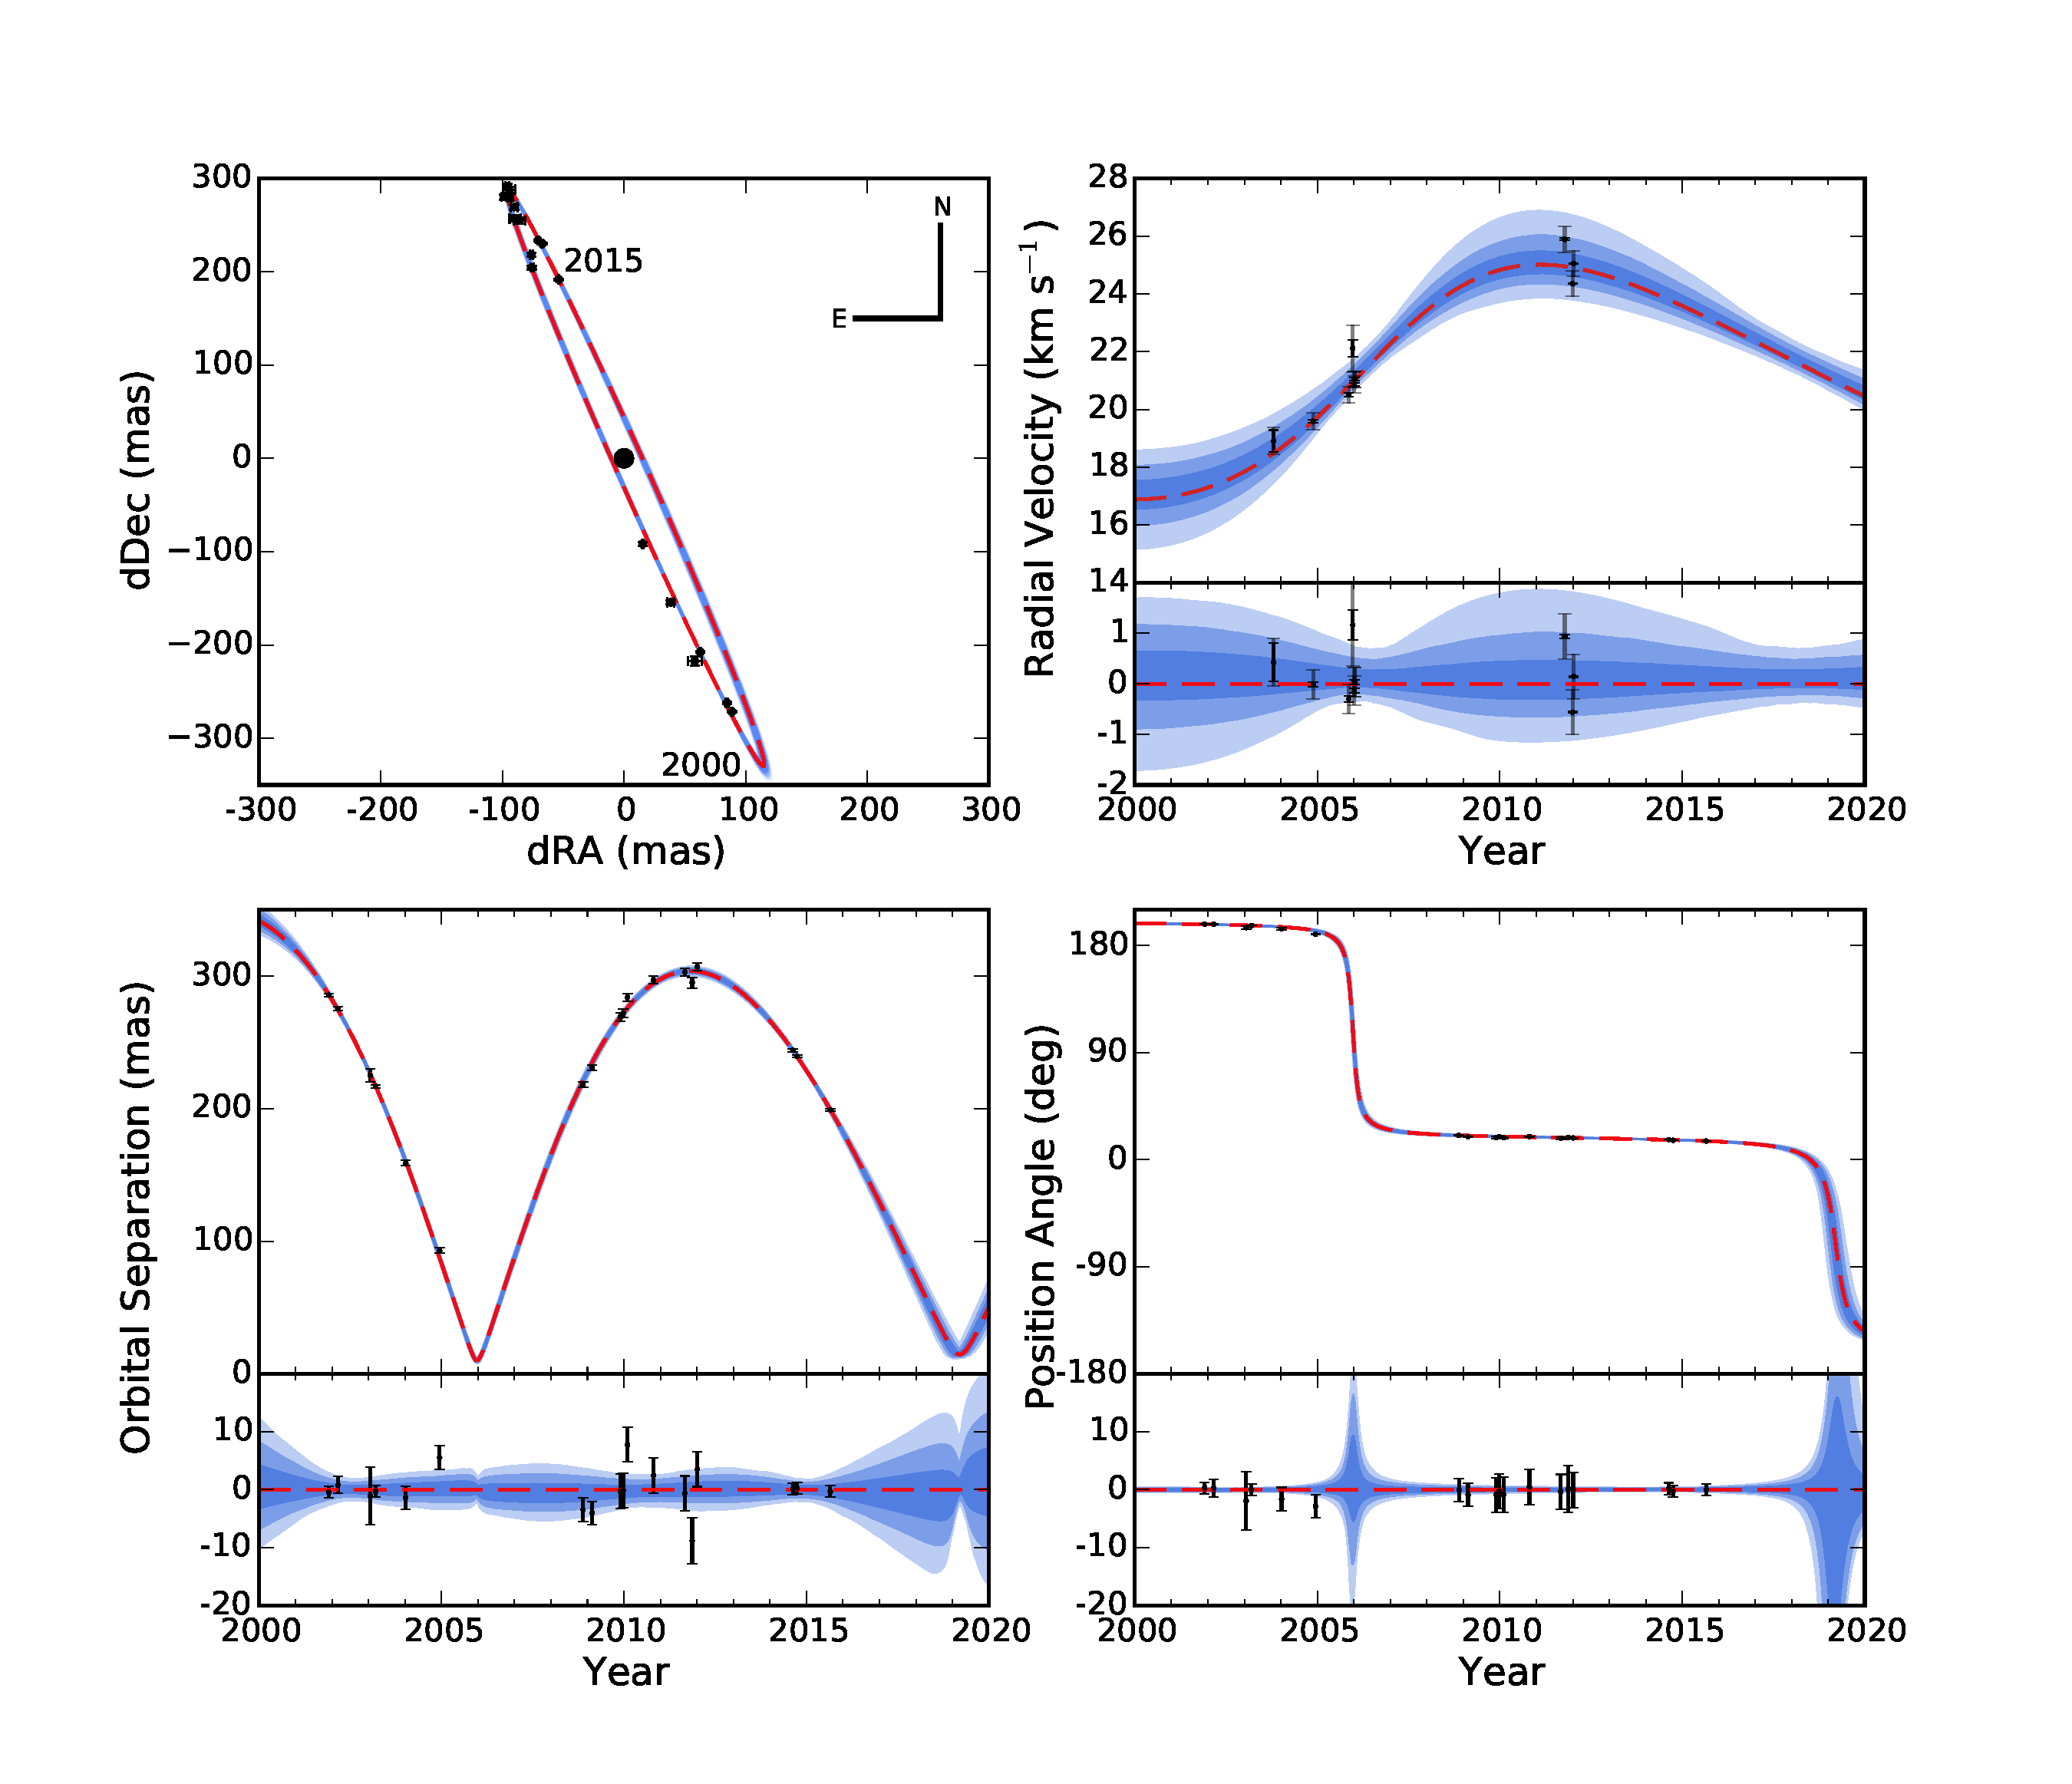
\includegraphics[width=0.85\textwidth]{chapter6/f1.pdf}}
\caption[Astrometry and RV data for \thisstarsix\,AB]{(Top Left) Astrometry for \thisstarsix\,AB. Data points correspond to the observations
listed in Table \ref{tab:astrometry}. Blue lines correspond to random draws from the posterior
distributions of orbital elements. The red, dashed line corresponds to the maximum likelihood
orbit. (Top Right) RV data for \thisstarsix\,A from the literature. 
The published uncertainties are in black;
in gray are the best-fitting uncertainties, incorporating an RV jitter model. The red, dashed
line corresponds to the maximum likelihood orbit. The blue shaded regions correspond
to the $1-$, $2-$, and $3\sigma$ uncertainties in the RV of \thisstarsix\,A.
(Bottom Left) Measured separations for \thisstarsix\,AB and residuals from the maximum likelihood
model. 
Each feature on the plot retains its meaning from the previous subplot.
(Bottom Right) Measured position angles for \thisstarsix\,AB and residuals from the maximum 
likelihood model.
  }
\label{fig:fits}
\end{figure}

We estimate bolometric luminosities for both of the stars in the system by integrating the CFHIST2011\_2015 model 
spectra of \citet{Baraffe15}.
We use the 3700 and 3500 K models with $\log g = 4.5$ (cgs) as spectral templates, scaling them
until they match the observed combined and differential magnitudes in each available bandpass.
We add in quadrature 0.10~mag of uncertainty in our visible-light magnitudes and 0.05~mag in 
the near-IR to account for stellar variability.

\section{Comparison with BHAC15 Evolutionary Models}
\label{sec:models}


Given the known distance to the system from \textit{Hipparcos} 
we can test if theoretical stellar evolution models
accurately predict the inferred stellar masses and age of the $\beta$ Pic moving group.
Combined-light photometry spanning from $B$ (0.4 $\mu$m) to $Ks$ (2.3 $\mu$m) was measured by the 
APASS, 2MASS, and \textit{WISE} surveys (Table~\ref{tab:photometry}).
We add an uncertainty of 0.03 mag in quadrature to the listed APASS uncertainties due to
the presence of systematics in APASS DR9 at that level \citep{Henden12}.
We also have obtained one epoch of differential photometry in two visible-light bandpasses with
DSSI and two near-IR bandpasses ($H$ and Br$\gamma$) with Keck/NIRC2.


\begin{table}[hbt!]
\centering
\begin{tabular}{lccc}
\hline
Bandpass & Source & Magnitude & Uncertainty \\
\hline
Combined & & & \\
$B$ &  APASS DR9 & 11.94 & 0.03  \\
$V$ &  APASS DR9 & 10.56 & 0.05 \\
$g'$ & APASS DR9 & 11.27 & 0.03 \\
$r'$ & APASS DR9 & 10.03 & 0.07 \\
$J$ &  2MASS & 7.30 & 0.02 \\
$H$ &  2MASS & 6.64 & 0.05 \\
$K$ &  2MASS & 6.41 & 0.02 \\
$W1$ & WISE & 6.34 & 0.03 \\
$W2$ & WISE & 6.21 & 0.02 \\
$W3$ & WISE & 6.16 & 0.02 \\
$W4$ & WISE & 6.00 & 0.04 \\
\hline
Resolved & & & \\
$\Delta$692 & DSSI & 1.89 & 0.04 \\
$\Delta$880 & DSSI & 1.17 & 0.03 \\
$\Delta$H$_2$ & Keck/NIRC2 & 1.00 & 0.02 \\
$\Delta$Br$\gamma$ & Keck/NIRC2 & 0.92 & 0.01 \\
$\Delta H$ & Keck/NIRC2 & 1.00 & 0.02 \\
\hline
\end{tabular}
\caption{Photometry for \thisstarsix\,AB}
\label{tab:photometry}
\end{table}

We compare the observed brightness of \thisstarsix\,AB to that predicted by the newest evolutionary models
of \citet{Baraffe15} for two stars of masses consistent with those inferred during our analysis
as a function of age. 
We find models of 25 Myr old stars accurately predict the combined-light near-IR flux for these
stars, although the models predict brighter $V$ magnitudes than those observed (Figure 2).
However, star $B$ is brighter than these same models predict: a 25 Myr old \thisstarsix\,B would be 
significantly brighter than what is observed. 
Assuming the stars are coeval, the models then predict a mass for \thisstarsix\,B that is 20\% lower 
than the observed mass. 

We create a simulated spectral energy distribution for each star, given the measured masses and the average age of 
$\beta$ Pic as measured from higher-mass stars. 
We interpolate absolute magnitudes predicted by the updated BHAC15 models of \citet{Baraffe15} along 
isochrones and isomass contours to predict apparent 
magnitudes for these stars in each bandpass.
We find that the total received flux is lower than
predicted by the BHAC15 models in each bandpass. While the flux for \thisstarsix\,A is consistent with 
the model predictions, \thisstarsix\,B is fainter than predicted.

Given the observed masses, we then vary the age of the system, assuming both stars are coeval, 
to determine which system age would be predicted by
these models given the observed combined and differential magnitudes.
We apply a flat prior on the age of the system, finding the BHAC15 models predict an age of $37 \pm 9$ Myr, consistent with the overall
age of the moving group \citep[$24 \pm 3$ Myr,][]{Bell15}.
As the system is unambiguously young, we can also confirm 51\,Eri\,b as 
a planetary mass object.


\begin{FPfigure}
\centerline{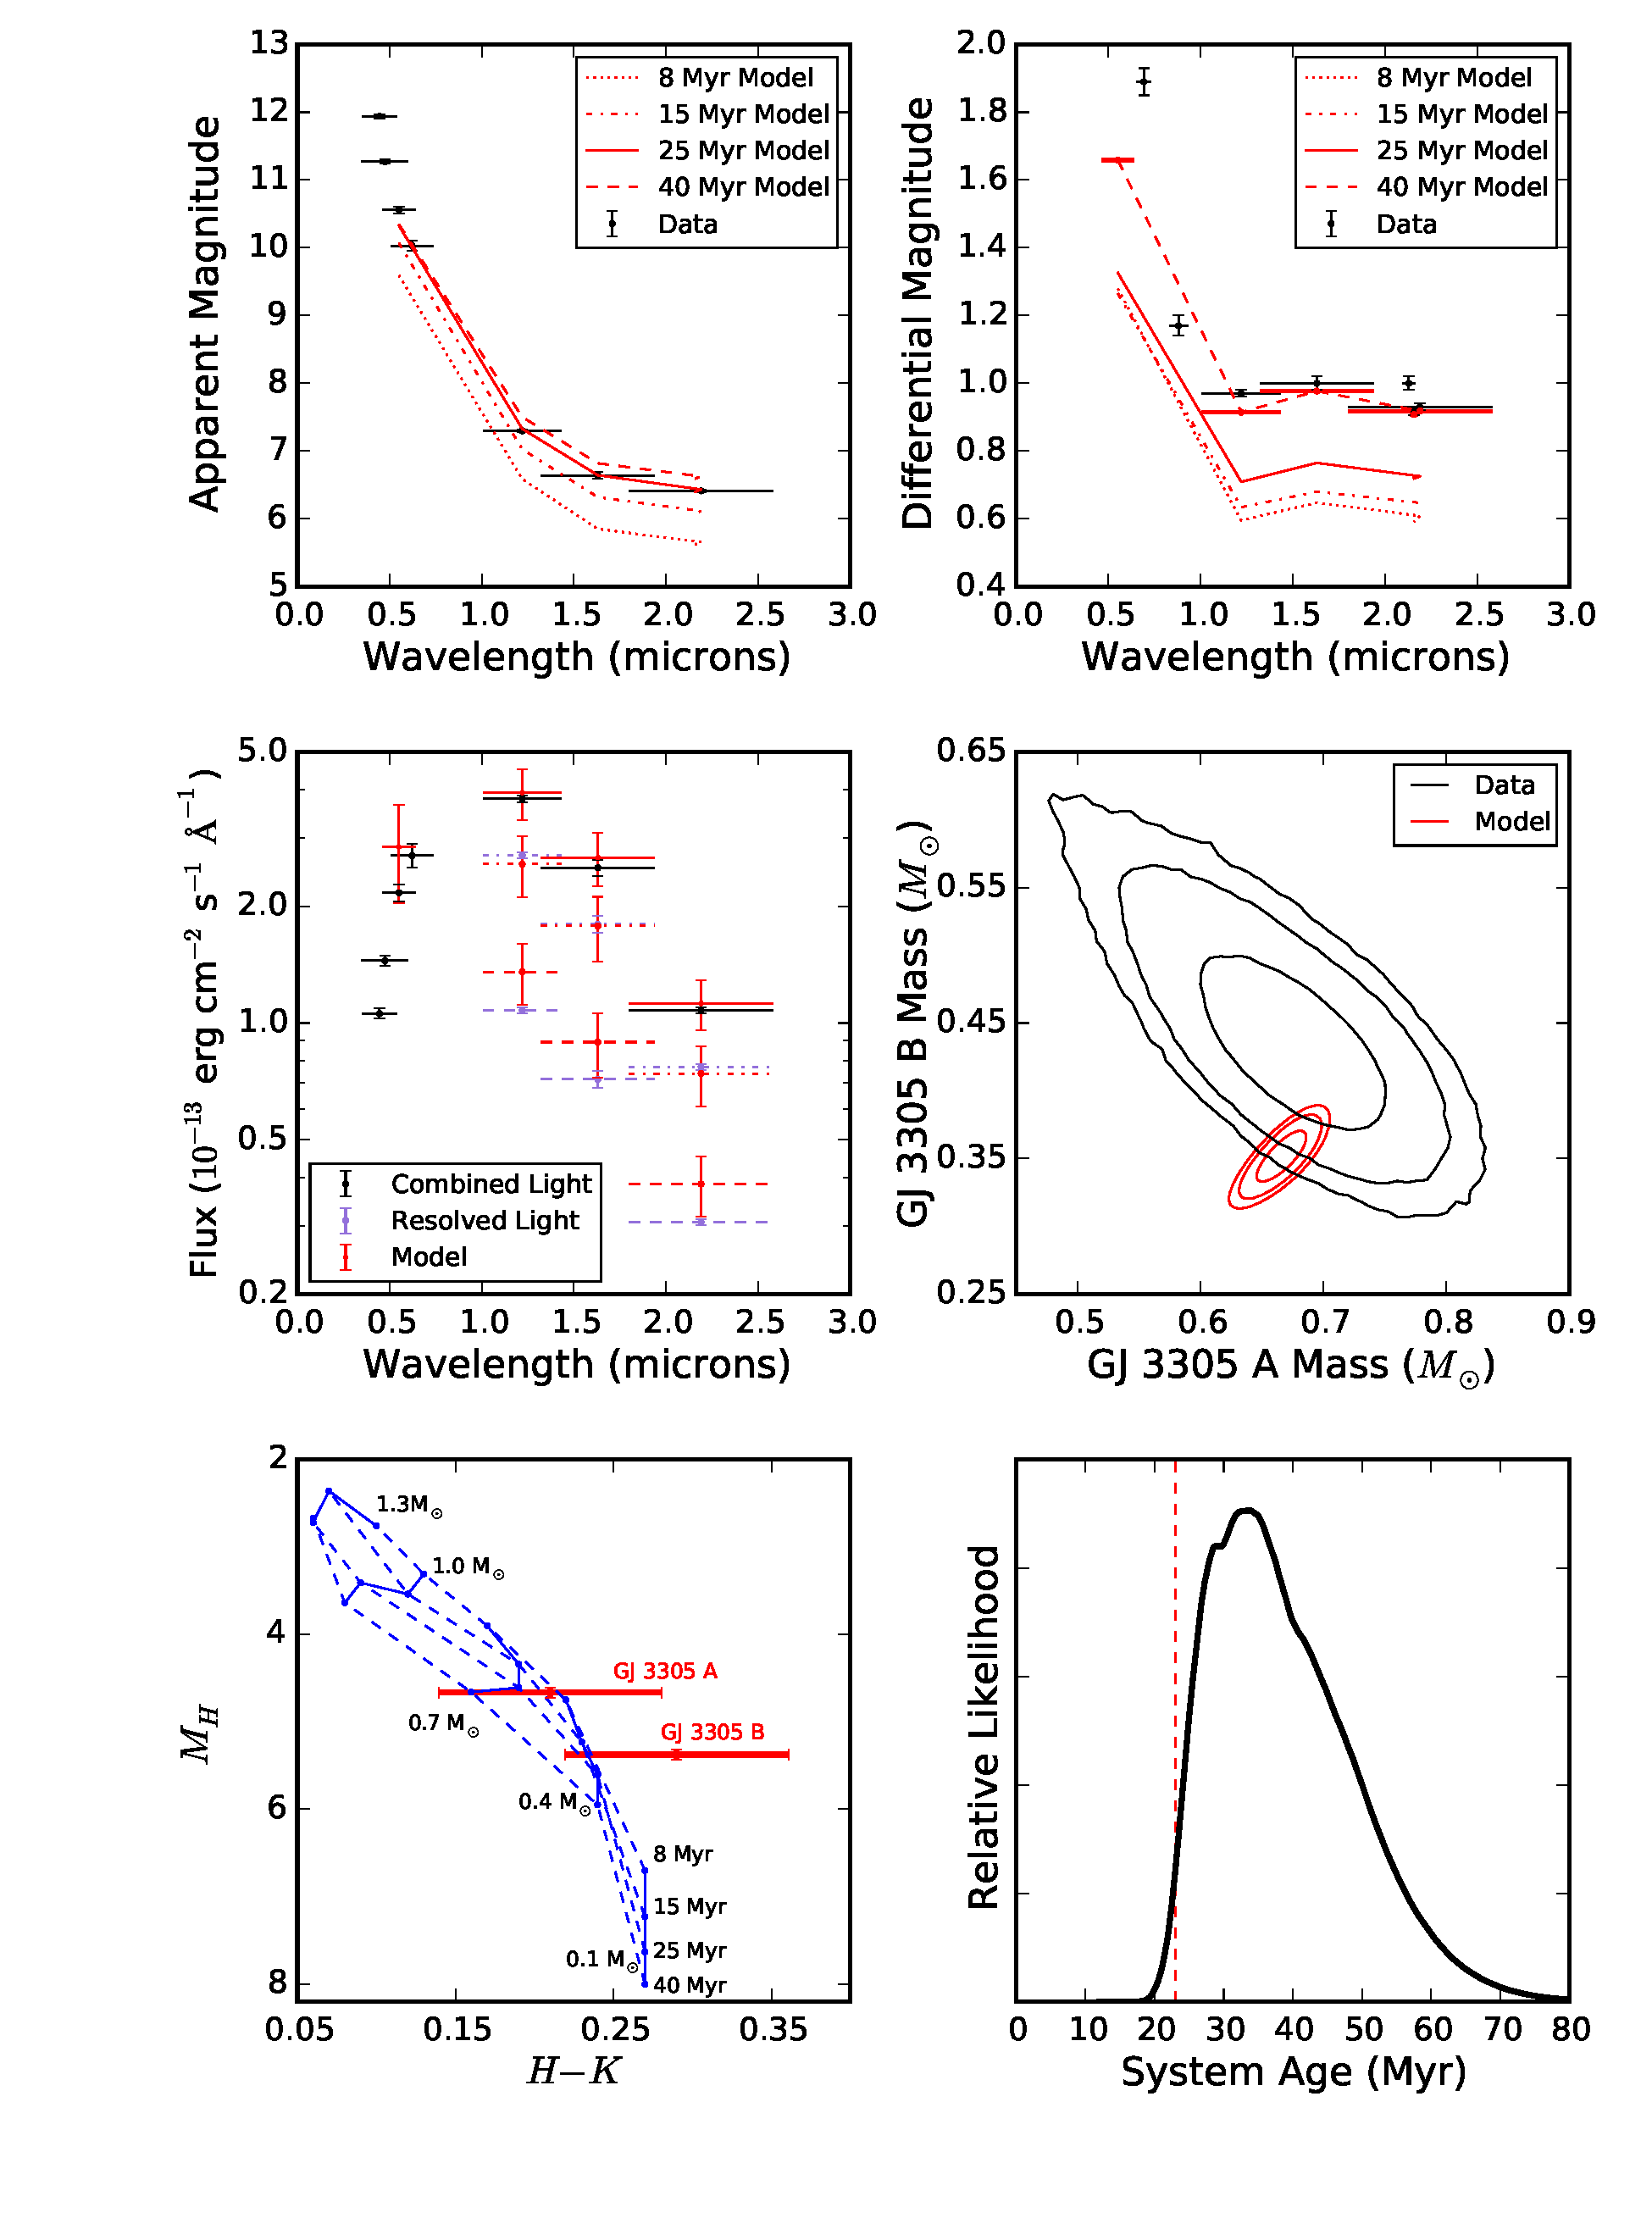
\includegraphics[width=0.95\textwidth]{chapter6/f2.pdf}}
\caption[Joint posterior probability distributions on the masses of \thisstarsix\,A and B, and comparison to the predictions
of theoretical models in color, luminosity, mass, and age]{(Top) (Left) Combined-light, unresolved and (Right) differential, resolved photometry for \thisstarsix\,AB (black) compared to
predictions (red) of the BHAC15 models as a function of age given the observed masses and parallax. The data are consistent with an age larger than 25 Myr.
Plotted bars along the abscissa correspond to the width of each filter and are meant to guide the eye: 
they do not represent an uncertainty.
(Middle left) SED for the system, assuming a $24 \pm 3$ Myr age and the observed masses. 
Combined-light photometry is in black and resolved photometry in purple. 
While the
model accurately reproduces the observed flux from \thisstarsix\,A, it overpredicts the received flux from 
\thisstarsix\,B.
(Middle right) Joint posterior probability distributions on the masses of the two stars,
(black) inferred from the astrometry and RV data and (red) predicted by the BHAC15 
models given the observed combined-light and differential photometry assuming
an age of $24 \pm 3$ Myr. Contours correspond
to the 1-, 2-, and 3-$\sigma$ confidence regions. The BHAC15 models predict a mass for
\thisstarsix\,B consistent with the mass inferred from the data, but underpredicts
the mass of \thisstarsix\,A by 20\%.
(Bottom left) CMD showing the absolute $H$ magnitudes and $H-K$ colors of \thisstarsix\,AB compared to theoretical
models. The models provide a more accurate fit for \thisstarsix\,A than \thisstarsix\,B.  
(Bottom right) Posterior probability distribution on the age of the \thisstarsix\ system, calculated by marginalizing the joint mass-age posterior over
all allowed masses, assuming both stars are the same age.
The BHAC15 models predict an age of $37 \pm 9$ Myr; the dashed line represents the \citet{Bell15} age of the $\beta$ Pictoris system.}
\label{fig:models}
\end{FPfigure}



\section{Discussion}


We have measured the masses and orbits of \thisstarsix\,AB, finding both to be 
consistent with the BHAC15 models at the $1.5\sigma$ level. 
In the future \thisstarsix\,AB and the gravitationally bound 51\,Eri\,Ab will be able to act as an isochronal test as a coeval,
co-metallicity quadruple system spanning stellar to planetary mass regimes.

The derived period of \thisstarsix\ ($29.03 \pm 0.50$ year) is longer than the 21 year found by \citet{Delorme12}.
The authors of that paper did not have sufficient data to fit all orbital parameters,
so they fixed the total system mass to $1.3$~\msun. Given our lower mass measurement, 
it is not surprising 
that our measured orbital period is longer. 

\subsection{Current Limitations}

It is possible that an unseen very low-mass star or brown dwarf orbiting
\thisstarsix\,B could cause us to overestimate its mass, causing the observed
$20\%$
discrepancy. 
For the system to be stable over $20$ Myr, such a companion would have to
be in a close ($P < 50$ day) orbit. 
The companion would then have to be in a nearly face-on ($i < 10^{\circ}$) orbit to evade RV detection.
Such companions could be found through continued astrometric monitoring of \thisstarsix. 
Such a companion would not affect our astrometry due to its small separation from \thisstarsix\,B
and would likely not affect our photometry due to its low luminosity relative to the other stars
in the system.

Most PMS M dwarfs have distance measurements to a precision no better than 5\%, meaning the 
total mass cannot be measured to better than 15\% \citep[e.g.][]{Shkolnik12}.
The uncertainty in the mass of \thisstarsix\,AB is only 4\%: the dominant source
of uncertainty in this value is the 1\% \textit{Hipparcos} parallax
to 51\,Eri,
making this system an ideal low-mass benchmark.
With a Gaia parallax forthcoming in the next few years, parallaxes for low-mass PMS stars will
be improved substantially.
Long-term astrometric and RV monitoring of wide M dwarfs is essential
as parallaxes are obtained over the next few years.

The uncertainty in the individual mass of each star is dominated by the uncertainty in the 
Doppler semiamplitude. 
While additional astrometric observations will not significantly improve the measured 
physical properties of \thisstarsix, additional RV observations will be important.
RV observations behind AO would be especially beneficial, as the RV from each 
star could be measured separately, instead of a flux-weighted RV centroid.




\subsection{Dynamical Effects on 51\,Eri\,b}


GJ 3305 AB and 51\,Eri\,Ab exist in a
dynamical configuration that may be susceptible to Kozai-Lidov
oscillations
\citep{Kozai62,Lidov62}, as suggested by \citet{Macintosh15}. 
In this scenario, the
planet-star binary (51\,Eri\,Ab) interacts secularly with \thisstarsix\,AB, 
leading to oscillations in inclination and eccentricity of the planet-star
sub-system. The timescale for such an interaction is
\begin{equation}
\tau \approx
P_\textrm{planet}\frac{M_\star}{M_\textrm{pert}}\bigg(\frac{a_\textrm{pert}}{a_\textrm{planet}}\bigg)^3(1-e_\textrm{pert}^2)^{3/2}
\end{equation}
where $P_{planet}$ is the orbital period of a planet with a semimajor
axis of $a_{planet}$ about a host of mass $M_\star$,
$M_\textrm{pert}$ is
the mass of a distant perturber, and $a_\textrm{pert}$ and $e_\textrm{pert}$
are the semimajor axis
and eccentricity of the perturber/planet-star ``binary'' orbit 
\citep[see e.g.][]{Holman97}.

Although we have limited information about this system, we can
estimate the time-scale for Kozai-Lidov cycles should the mutual
inclination of the 51\,Eri\,Ab system and (51\,Eri\,Ab)-(\thisstarsix\,AB)
system satisfy $ 140^\circ \lesssim i_m  \gtrsim 40^\circ$. 
Taking the instantaneous sky-projected separations as a
proxy for the semimajor axes and inferred masses of
$M_\star=1.75$~\msun\  \citep{Simon11} and $M_\textrm{pert} = 1.1$~\msun\ yields a
timescale of
$\tau \sim 2\times10^8 \textrm{ yr }(1-e_\textrm{pert}^2)^{3/2}$.
Therefore, unless the eccentricity
of \thisstarsix\ about the 51\,Eri subsystem satisfies
$e_\textrm{pert}\gtrsim 0.9$, the timescale for Kozai-Lidov oscillations
is longer than the age of the system,
so we do not expect the Kozai-Lidov mechanism to have had
time to induce a large eccentricity or spin-orbit misalignment
within the 51\,Eri sub-system. If future
observations indicate non-zero spin-orbit misalignment or a high
eccentricity for the orbit of 51\,Eri\,b, a primordial origin unrelated to
the distant perturbers would be suggested.




\chapter{Stellar and Planetary Properties of \KT\ Campaign~1 Candidates and Validation of 17 Planets, Including a Planet Receiving Earth-like Insolation}
\label{chap:k2}
In the final two science chapters I turn my attention to large surveys. The first of these is \KT\ the extended \kep\ mission.
The large systematics inherent to \KT\ data make detecting planets more challenging than in \kep; the stellar target list is
put together only months before each field as a conglomeration of many other catalogs, making stellar parameters uncertain
and potentially systematically biased.
Here, we attempt to solve both of these issues.
Following a systematic search for transiting planets, we combine RV data, AO imaging, and archival data on the stars to
better infer stellar parameters and statistically validate the transiting planets, applying our methods to Campaign 1 of the
\KT\ mission.
We validate 17 planets, including one which receives an Earth-like level of insolation and has an equilibrium temperature of $272 \pm 15$ K.
This chapter was originally published as ``Stellar and Planetary Properties of K2 Campaign 1 Candidates and Validation of 17 Planets, Including a Planet Receiving Earth-like Insolation,'' ApJ, 809, 25 (2015) by BTM, Tim Morton, Dan Foreman-Mackey,
John Johnson, David Hogg, Brendan Bowler, Dave Latham, Allyson Bieryla, and Andrew Mann.



\section{Introduction}
The \kep\ telescope \citep{Borucki10} has led to a revolution in stellar and planetary
astrophysics, with 7305 ``objects of interest'' and 4173 ``planet candidates''
discovered to date \citep{Borucki11a, Borucki11b, Batalha13, Burke14, Rowe15, Mullally15}.
The fidelity of this sample is high: most of these candidates are truly planets
\citep{Morton11b, Fressin13, Desert15}.
The mechanical failure of two reaction wheels on the spacecraft led to a repurposing
of the spacecraft into the \KT\ mission, in which the telescope points at
fields near the ecliptic plane for $\sim 75$ days at a time \citep{Howell14}.
In this observing strategy, two axes of motion of the spacecraft are
controlled by the two remaining reaction wheels, while the roll of the
spacecraft is balanced with Solar radiation pressure and quasiperiodic
thruster firing.
As a result, the detector drifts relative to the sky
at the rate of $\sim 1$ arcsec hr$^{-1}$, with rapid corrections due to thruster fires
approximately once every six hours.
Over the full duration of each campaign, the targets remain near the
same location on the detector but both the slow drift and the corrections are
observable by eye \citep{Barentsen15}.

\KT\ light curves produced with aperture photometry contain substantial pointing-induced
photometric variations caused by the star's apparent motion over a poorly-defined flat
field.
Worse yet, these variations occur on timescales similar to transit signals, potentially
masking the observational signature of a planet passing between \kep\ and its host star.

There has been considerable effort to recover these planetary signals, and to date six
planets have been confirmed orbiting three stars in the \KT\ data
\citep{Vanderburg15, Crossfield15, Armstrong15b}.
What is common to all of these methods are that removal of systematics is considered a
step to be undertaken before the search for planets.
Under this strategy, it is implicitly assumed that the systematics are removed perfectly,
while retaining all of the astrophysical signal.
Of course, it is impossible to perfectly separate the astrophysical and instrumental
signal, and such a technique is prone to either over-fitting, in which some of the
astrophysical signal is also removed, or under-fitting, in which some
of the instrumental systematics remain.
A better strategy is to simultaneously fit both the signal and the systematics, as is common
practice in cosmology and, increasingly, in radial velocity searches for planetary systems
\citep[e.g.][]{Ferreira00, Boisse11, Haywood14, Grunblatt15}.

\paperit{} simultaneously fit both the systematics and potential planetary transit signals
in a search for transiting planets.
They assume that the dominant trends in the observed stellar light
curves are caused by spacecraft motion and are shared by many stars.
They then run PCA on all stars to measure the dominant modes, modeling each star as a
linear combination of 150 of these ``eigen light curves'' and a transit signal.
This method enables fitting without over-fitting, and also permits marginalization over
uncertainties induced by the systematic model.
Therefore, any uncertainties in the systematics can be propagated into uncertainties in
detected planet parameters, instead of assuming the systematics are understood perfectly.
Using this technique, \paperit{} detect 36 planet candidates orbiting 31 stars in \KT\
\Ci\ data.

In \paperit, only transit properties are provided, not absolute parameters about the
planet or the star.
Additionally, the authors follow the convention of the \kep\ team to include any
transit event as a candidate system rather than a false positive if a secondary eclipse
is not detected: there is no enforced upper limit on the allowed planet radius.
The authors intentionally make no effort to separate true transiting planets from
astrophysical events that mimic the appearance of transits, such as an eclipsing
binary with a high mass ratio, similar to the \kep\ team's list of ``objects of interest.''


In this paper, we present stellar and planetary parameters for each system.
We also analyze the false positive probability of each system using \texttt{vespa},
a new publicly available, general-purpose implementation
of the \citet{Morton12} procedure
to calculate false positive probabilities (FPPs) for transiting planets.
Through this analysis, as well as archival imaging, ground-based
seeing-limited survey data, and adaptive optics imaging, we are able to confirm
\Nvalidated\ of these systems as transiting planets at the 99\% confidence
level.
Additionally, we identify six systems as false positives.

This paper is organized as follows.
In \textsection2, we develop stellar properties through
photometric and spectroscopic data.
In \textsection3, we combine the derived stellar properties with \KT\ data to infer planet
candidate properties.
In \textsection4, we combine adaptive optics and radial velocity observations with both
archival and modern ground-based, seeing limited survey data and an analysis of the
transit parameters to calculate false positive probabilities.
In \textsection5, we discuss potentially interesting systems, including a mini-Neptune
orbiting an M dwarf which receives a similar insolation to the Earth.
In \textsection6, we summarize and discuss our results.


\section{Stellar Properties}
\subsection{Photometry}

With the exception of one star in our sample (K2-18), we do not have
spectroscopic data with which to characterize the stellar properties.
Additionally, there are no measured parallaxes for any of these stars.
Instead, we rely on photometry.
For each system, we query the VizieR database of astronomical catalogues
\citep{Ochseinbein00}.
We record the $B$, $V$, $g'$, $r'$, and $i'$ magnitudes and their
uncertainties from the AAVSO Photometric All-Sky Survey (APASS) DR6
\citep{Henden14}, as reported in the UCAC4 Catalogue \citep{Zacharias12}.
We also record the $J$, $H$, and $K$ magnitudes and their uncertainties
as found in the 2MASS All-Sky Catalog of Point Sources \citep{Cutri03}
and the $W1-W3$ WISE magnitudes and uncertainties from the ALLWise Data
Release \citep{Cutri13}.
For all except two of our targets, the $W4$ band is only an upper limit,
and in the remaining two cases, the photometric uncertainity in $W4$ is at least an
order of magnitude larger than those in $W1-W3$, so we do not use $W4$
for any system.
These data are reported in Table 7.1, and a color-color diagram showing the
$r-J, J-K$ colors of our candidates is included as Fig.~\ref{fig:photometry}.

\begin{figure}[htbp]
\centerline{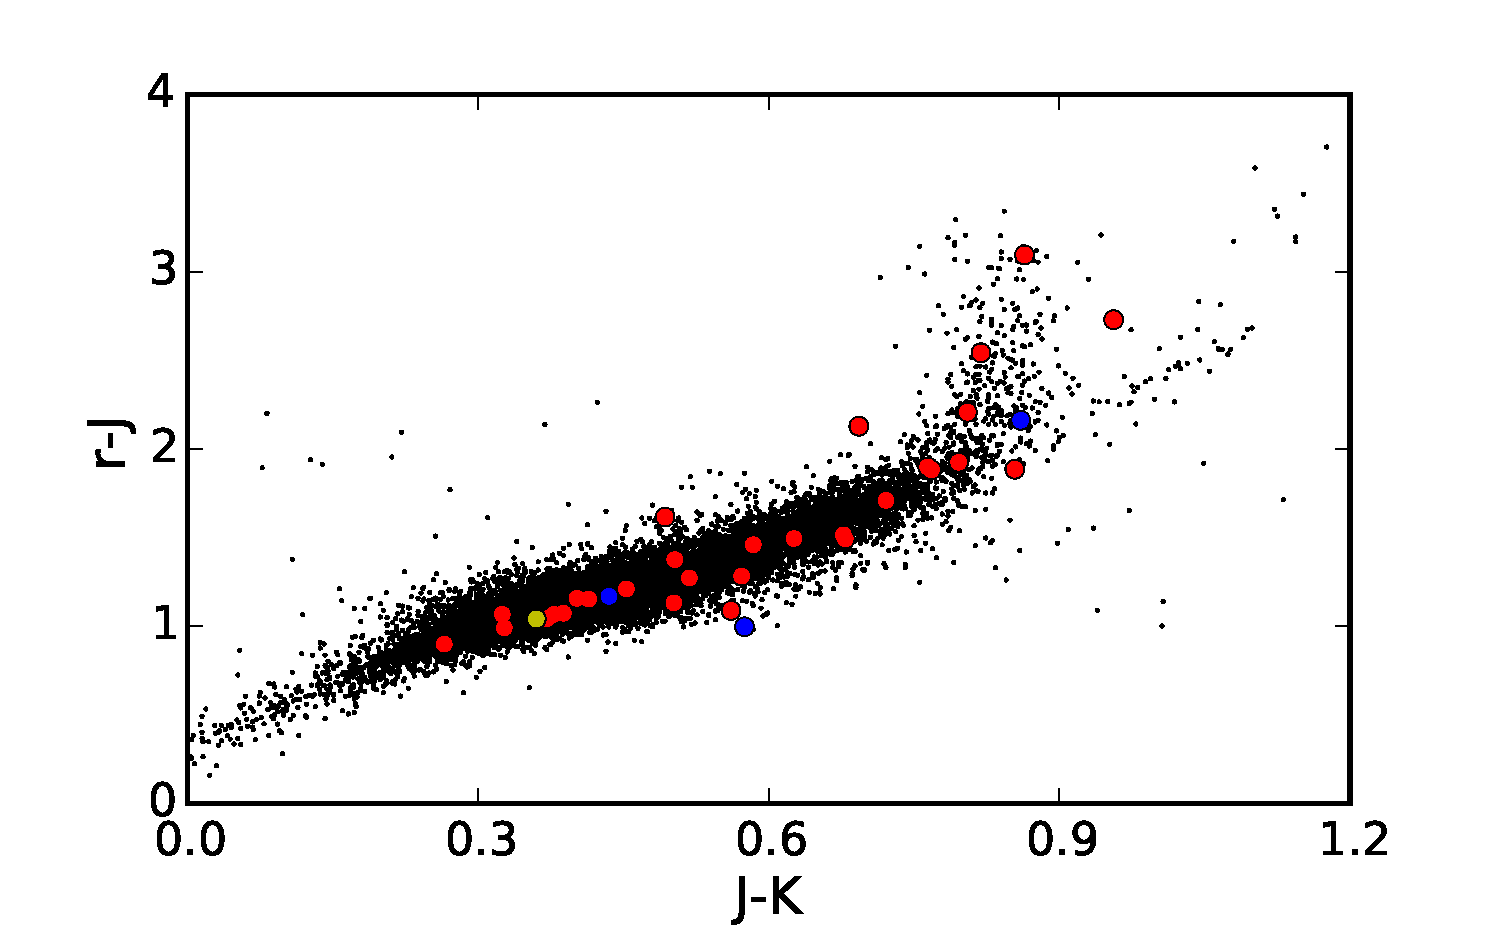
\includegraphics[width=0.75\textwidth]{chapter7/f1.pdf}}
\caption[Color-color diagram showing \kep\ targets with our own \KT\ planet candidates overlaid.]
{Color-color diagram displaying $r-J, J-K$ photometry for targets
observed by \kep\ during the original
mission (black), with our \KT\ \Ci\ planet candidates overlaid (red).
Also included is the location of the Sun (yellow) and host stars of previously
confirmed \KT\ planets (blue).
90\% of our candidates have photometry consistent with later spectral
types than the Sun.}
\label{fig:photometry}
\end{figure}


\subsection{Stellar Models}
\label{sec:stellarparams}
To convert the observed photometric data into physical properties for each
star, we used the new publicly available \texttt{isochrones} Python module\footnote{
\url{http://github.com/timothydmorton/isochrones}}, a general-purpose
interpolation tool for the fitting of stellar models to photometric or spectroscopic
parameters \citep{Morton15a}.
This software does trilinear interpolation in mass--age--\feh\ space for any
given set of model grids, thus being able to predict the value for any
physical or photometric property provided by the models at any values of
mass, age, and \feh\ within the boundaries of the grid.

This enables a set of observed properties ($\left\{ x_i, \sigma_i \right\}$),
either spectroscopic, photometric,
or both, to define a likelihood function to be sampled:
\begin{equation}
\label{eq:ischochronelhood}
\ln \mathcal L(\boldsymbol{\theta}) \propto -\frac{1}{2} \displaystyle \sum_i \frac{\left(x_i -
  I_i\left(\boldsymbol{\theta} \right)\right)^2}{\sigma_i^2},
\end{equation}
where $I_i(\boldsymbol{\theta})$ is the isochrone model prediction of property
$i$ at the given parameters $\boldsymbol{\theta}$.
If the observed properties include any apparent magnitudes, then
$\boldsymbol{\theta}$ includes distance and extinction in addition
to mass, age, and \feh.

In this work, we use grids from the Dartmouth Stellar
Evolution Database \citep{Dotter08} at Solar values of \afe=$0.0$ and
helium abundance $Y=0.2741$, which come packaged with the \texttt{isochrones}
module.
We then infer the stellar parameters using \texttt{MULTINEST} \citep{Feroz09},
an implementation of a multimodal nested sampling algorithm,
for each host star conditioned on the observed
photometric properties as presented in Table 7.1.
\texttt{MULTINEST} is designed to sample multimodal posteriors, where other 
samplers such as MCMC algorithms often struggle. 
Given the multimodal nature of our posteriors, this scheme is optimal for 
capturing parameter space on the subgiant branch where these stars could reside.
We include a prior on stellar metallicity representative of the observed metallicities
of stars within 1 kpc of the Sun, following the results of \citet{Hayden15}, and a Salpeter-slope
prior on mass up to the maximum mass available in the model grids of $3.7$ $M_\odot$.

During the sampling process, we fit for Galactic
extinction as one of our physical parameters.
We include the WISE bandpasses by applying the relative extinction values between
SDSS, 2MASS, and WISE calculated by \citet{Davenport14}.
In each step of our fitting process, we draw a value for $A_V$, calculate the expected extinction
in all bandpasses $A_X$ assuming the $R_V = 3.1$ reddening law of \citep{Fitzpatrick99}, 
and then measure the likelihood of our model stellar fit to the observed apparent magnitudes.
We apply a uniform prior ranging from zero to a maximum extinction value of 0.2 and
marginalize over extinction in our final determination of stellar parameters.
The NASA/IPAC Extragalactic Database (NED), which reports the
\citet{Schlafly11} recalibration of the \citet{Schlegel98} extinction map as measured by
COBE/DIRBE and IRAS/ISSA, suggests that typical $A_V$ extinction values to the edge
of the galaxy at this
high Galactic latitude are $\sim$0.1 magnitudes, so our upper limit appears to be justified.

Such a scheme enables us to infer the statistical uncertainties on the
mass, radius, and effective temperature.
However, we are subject to biases induced by systematics in the models themselves.
There is some evidence that the Dartmouth models may under-predict
radii of M dwarfs by $\sim 15\%$ when compared to other methods \citep{Newton15,
Montet15a}.
Such an effect may be the result of the Dartmouth model reliance on BT-Settl
atmospheres, which are based on incomplete molecular line lists and
have been shown to predict near-IR colors that are too blue
\citep{Thompson14}.

As our stellar results are model-dependent, we caution users who intend to use these
parameters for other works, such as exoplanet population studies. When available,
stellar parameters inferred through other techniques such as asteroseismology or
spectroscopy should supersede these values.
We note the observed photometric parameters are consistent with spectroscopically-derived
parameters for stars with published spectra, and consistent with typical
model-dependent uncertainties
from photometric data \citep[e.g.][]{Huber14}.
We provide full samples of our posteriors on the physical parameters for each
star\footnote{\url{http://www.astro.princeton.edu/~tdm/k2/}}.

\citet{Bastien14} use the ``granulation flicker'' in the \kep\ light curves
to suggest that
approximately 50 percent of planet host stars have evolved off the
main sequence onto the subgiant branch, so that both the host stars and their
planets are larger than previously reported.
Similarly, in \KT\ \Ci\ we may expect to find evolved stars in a sample of planet
candidates, although we may expect the effect to be lessened due to the
high Galactic latitude of \Ci.
Indeed, we find this to be the case.
Two stars, EPIC 201257461 and 201649426 are definitively evolved stars,
with inferred masses less than 2 \msun but radii above 8 \rsun.
For approximately one third of the others,
we find the stellar radius posterior distribution to be bimodal, with both main
sequence and subgiant models of the stars being consistent with the photometric
data.
This number is consistent with our expectations of the number of subgiant
contaminants in the \Ci\ field (K. Stassun, private communication).
Future observations to measure the parallaxes of these stars, such as with Gaia,
will be helpful in differentiating between these two models to determine
more precisely the stellar, and thus the planetary, radii.






\subsection{SNIFS and SpeX Spectroscopy}
\label{Spexobs}


A near-infrared spectrum of K2-18 was obtained using the upgraded SpeX
(uSpeX) spectrograph \citep{Rayner03} on the NASA Infrared Telescope Facility
(IRTF) on January 29 2015 (UT).
SpeX observations were taking using the short cross-dispersed mode and the
0.3$\times15$ arcsec slit, which provides simultaneous coverage from 0.7
to 2.5$\mu$m at $R\simeq2000$.
The target was observed at two positions along the slit to subsequently subtract
the sky background. Eight spectra were taking following this pattern, which provided
a final S/N of $>150$ per resolving element.
The spectrum was flat fielded, extracted, wavelength calibrated, and stacked
using the \textit{Spextool} package \citep{Cushing04}.
An A0V-type star was observed immediately after
the target, which was used to create a telluric correction using the
\textit{xtellcor} package \citep{Vacca03}.

An optical spectrum was obtained using the SuperNova Integral Field Spectrograph
\citep[SNIFS,][]{Aldering02,Lantz04} on the University of Hawai'i
2.2m telescope on the night of January 30 2015.
SNIFS provides simultaneous coverage from 3200\AA--9700\AA\ at a resolution
of $\simeq1000$. Final S/N of the spectrum was $>100$ per resolving element
in the red ($\sim6000$\AA).
Details of the SNIFS reduction, including dark, bias, and flat-field corrections,
cleaning the data of bad pixels and cosmic rays, and extraction of the
one-dimensional spectrum are described in \citet{Bacon01} and
\citet{Aldering06}.
Flux calibration was performed using a separate pipeline described in \citet{Mann15}.

\teff\ was calculated by comparing our optical spectra with the CFIST
suite\footnote{\url{http://phoenix.ens-lyon.fr/Grids/BT-Settl/CIFIST2011/}} of the BT-SETTL
version of the PHOENIX atmosphere models \citep{Allard13}, which gave a temperature
of 3503 $\pm$ 60\,K.
More details of this procedure are given in \citet{Mann14} and
\citet{Gaidos14}.
This method was used because it is known to accurately reproduce empirical
\teff\ values from long-baseline optical interferometry \citet{Boyajian12}.

Metallcity was determined using the procedures from \citet{Mann13a}, in which the
authors provide empirical relations between atomic features and M dwarf
metallicity, calibrated using wide binaries.
We adopted the weighted mean of the $H-$ and $K-$band calibrations,
which yielded a metallicity of 0.09$\pm$0.09.

We combined the derived \teff\ and [Fe/H] values with the empirical
\teff-[Fe/H]-$R_*$ relation from \citet{Mann15} to compute a radius.
Accounting for measurement and calibration errors in [Fe/H] and \teff\ we calculated
a radius 0.394$\pm0.038R_\odot$.
We use these parameters instead of the derived photometric properties for this target,
although we note the two are consistent at the $1\sigma$ level.

The full list of stellar parameters adopted in this paper is included in
Table 7.2.
% For some reason I can't get it to identify the table \ref here.
% If anyone can figure it out, be my guest!

\section{Planet Properties}

In \paperit, only parameters directly observable from the \KT\ light curve
itself were reported: the period, time of transit center, and transit depth.
With stellar properties now in hand, we can convert these observational
results into fundamental parameters of each planet candidate.
For each candidate, we fit the light curve using a physical transit model
\citep{Mandel02, Kipping10b} simultaneously with a systematics model similar
to the one described by \paperit.
We use \texttt{emcee} \citep{Foreman-Mackey12}, an implementation of the
affine-invariant ensemble sampler of \citet{Goodman10}
 to sample from the posterior probability distribution
for the stellar---limb darkening coefficients, mass, radius, and effective
temperature---and planetary---radius, period, phase, impact parameter,
eccentricity, and argument of periapsis---parameters, conditioned on the
light curve and the measured stellar properties.


Following \paperit, the likelihood function that we use is marginalized over
the weights of the ``eigen light curves'' in the linear systematics model.
Unlike \paperit, we include an empirical Gaussian prior on the weights
determined by robustly computing the distribution of weights across the full
set of Campaign~1 light curves.
This prior mitigates the incorrect detection of false signals induced by
stellar variability---as discussed below in Section~\ref{sec:systematics}---so
we exclude these candidates (EPIC 201929294 and EPIC 201555883) from the tables
of results.


In this analysis, we assume the dilution caused by additional stars
contributing flux into the aperture is negligible for nearly all systems.
Given the location of the \Ci\ field at a high Galactic latitude, we expect
low contamination by background giants.
Nevertheless, this assumption may not be valid for all systems.
Any contamination unaccounted for, as may happen if any of these stars are
actually unresolved binaries, would cause us to underestimate the radii of any
planets we detect.
Therefore, high-contrast adaptive optics imaging of any systems should be
obtained before these planets are used in population inference studies.
The planet parameters measured by this analysis are listed in Table 7.3.



\section{False Positive Analysis}


There are many scenarios which can cause an astrophysical false positive,
where an eclipsing binary star masquerades as a transiting planet.
The most common scenarios are if (a) it is a highly grazing eclipse, or (b) the binary system
shares a photometric aperture with a significantly brighter star,
resulting in a diluted eclipse depth.
When possible, such astrophyscial false positive scenarios are traditionally
ruled out by detailed follow-up observations, often a combination of
high-resolution imaging and radial-velocity measurements.
However, the \kep\ mission, with its thousands of planet candidates
around mostly faint stars, necessitated a paradigm shift---a move
toward probabilistic interpretation of transit signals, rather than
comprehensive follow-up of each individual candidate \citep{Morton11b}.

\citet{Morton12} presented an automated method to calculate the
probability that a planet candidate might be caused by an
astrophysical false positive.
This method uses Galactic population simulations to determine the
distributions of possible false positive scenarios, comparing the
typical light curve shape of each to the data.
It then combines this information with observationally motivated prior
assumptions about the populations of field stars, the properties of
multiple star systems, and the occurrence rate of planets as determined
from \kep\ \citep{Fressin13}, in order to determine the probability that
the observed signal may be a false positive.
Similar in spirit to other published methods of
probabilistic validation, such as BLENDER \citep{Torres11a} and PASTIS
\citep{Diaz14a}, it has the advantage of being computationally less demanding
and fully automated, and thus easily applied in batch to a large
number of candidates.

In this work, we use
\texttt{vespa}\footnote{\url{http://github.com/timothydmorton/vespa}} \citep{Morton15b},
a new publicly available, general-purpose implementation
of the \citet{Morton12} procedure,
to calculate false positive probabilities (FPPs) for each of these
\KT\ candidates.
The following constraints on false positive
scenarios are imposed:
\begin{itemize}
\item A chance-aligned eclipsing binary system may reside anywhere inside
or within one pixel of the photometric aperture of the target star.
In creating a light curve for each star, we define photometric apertures ranging
from 10 to 20 arcseconds for each star, as defined in Table 7.4.
Given the 6-arcsecond PSF of the \kep\ telescope, we allow for the possibility
that companions falling just outside of our aperture (within one pixel) may
contribute to the light curve, possibly causing a false positive event.
The search for such companions is discussed in
\textsection \ref{sec:background}.
\item The maximum allowed depth of a potential secondary eclipse event
is the most significantly detected signal at the same
period of the planet candidate, once the primary transit is masked out
(discussed in \textsection\ref{sec:sec}).
\texttt{vespa} does not allow for the possibility of secondary eclipses
larger than those observed in the \KT\ light curve for each star.
\item Blended stars must be allowed by the available adaptive optics
and archival imaging data (discussed in detail in \textsection
\ref{sec:AO} and \ref{sec:background}).
\texttt{vespa} only considers stars below the detection threshold for
the AO imaging, which is a position-dependent value following a calculated
contrast curve for each star.
\end{itemize}

Each of these scenarios is an astrophysical eclipse, caused by one
object passing in front of another, blocking some fraction of the
total light.
The calculations here do not include the possibility
that each signal is caused by an instrumental artifact in the data or
some other astrophysical event, such as stellar activity, masquerading
as planet transits.

Table 7.5 summarizes the results of these
calculations, presenting the relative probability for each candidate
to be caused by any of three false positive scenarios: an undiluted
eclipsing binary (EB), a hierarchical triple eclipsing binary (HEB),
and a chance-aligned background(/foreground) eclipsing binary (BEB).

Six of the presented candidates have FPP $>$90\%;
these are considered to be likely false positives.
On the other hand, 24 candidates
have FPP $<$ 1\%.
Three of the transit signals might plausibly be caused by
contamination by detected stellar companions within the photometric apertures
(see \S\ref{sec:background}), so we keep these as candidates.

This leaves 21 candidates that we statistically validate as planets, including
four that have been previously
identified in the literature \citep{Crossfield15, Armstrong15b}.
So in total, of the 36 candidates, 21 are secure planets,
17 of which we validate here for the first time.


We emphasize that the majority of these validations rely
solely on the transit photometry and SDSS data, with follow-up imaging only obtained for
seven of the 31 targets.  This
demonstrates the utility of the \texttt{vespa} tool, which will be
crucial to interpreting future candidates detected by \KT, TESS, and PLATO
and prioritizing follow-up observing efforts.
We show the transit signals in Figure~\ref{fig:transits}.

\begin{figure}[htbp]
\centerline{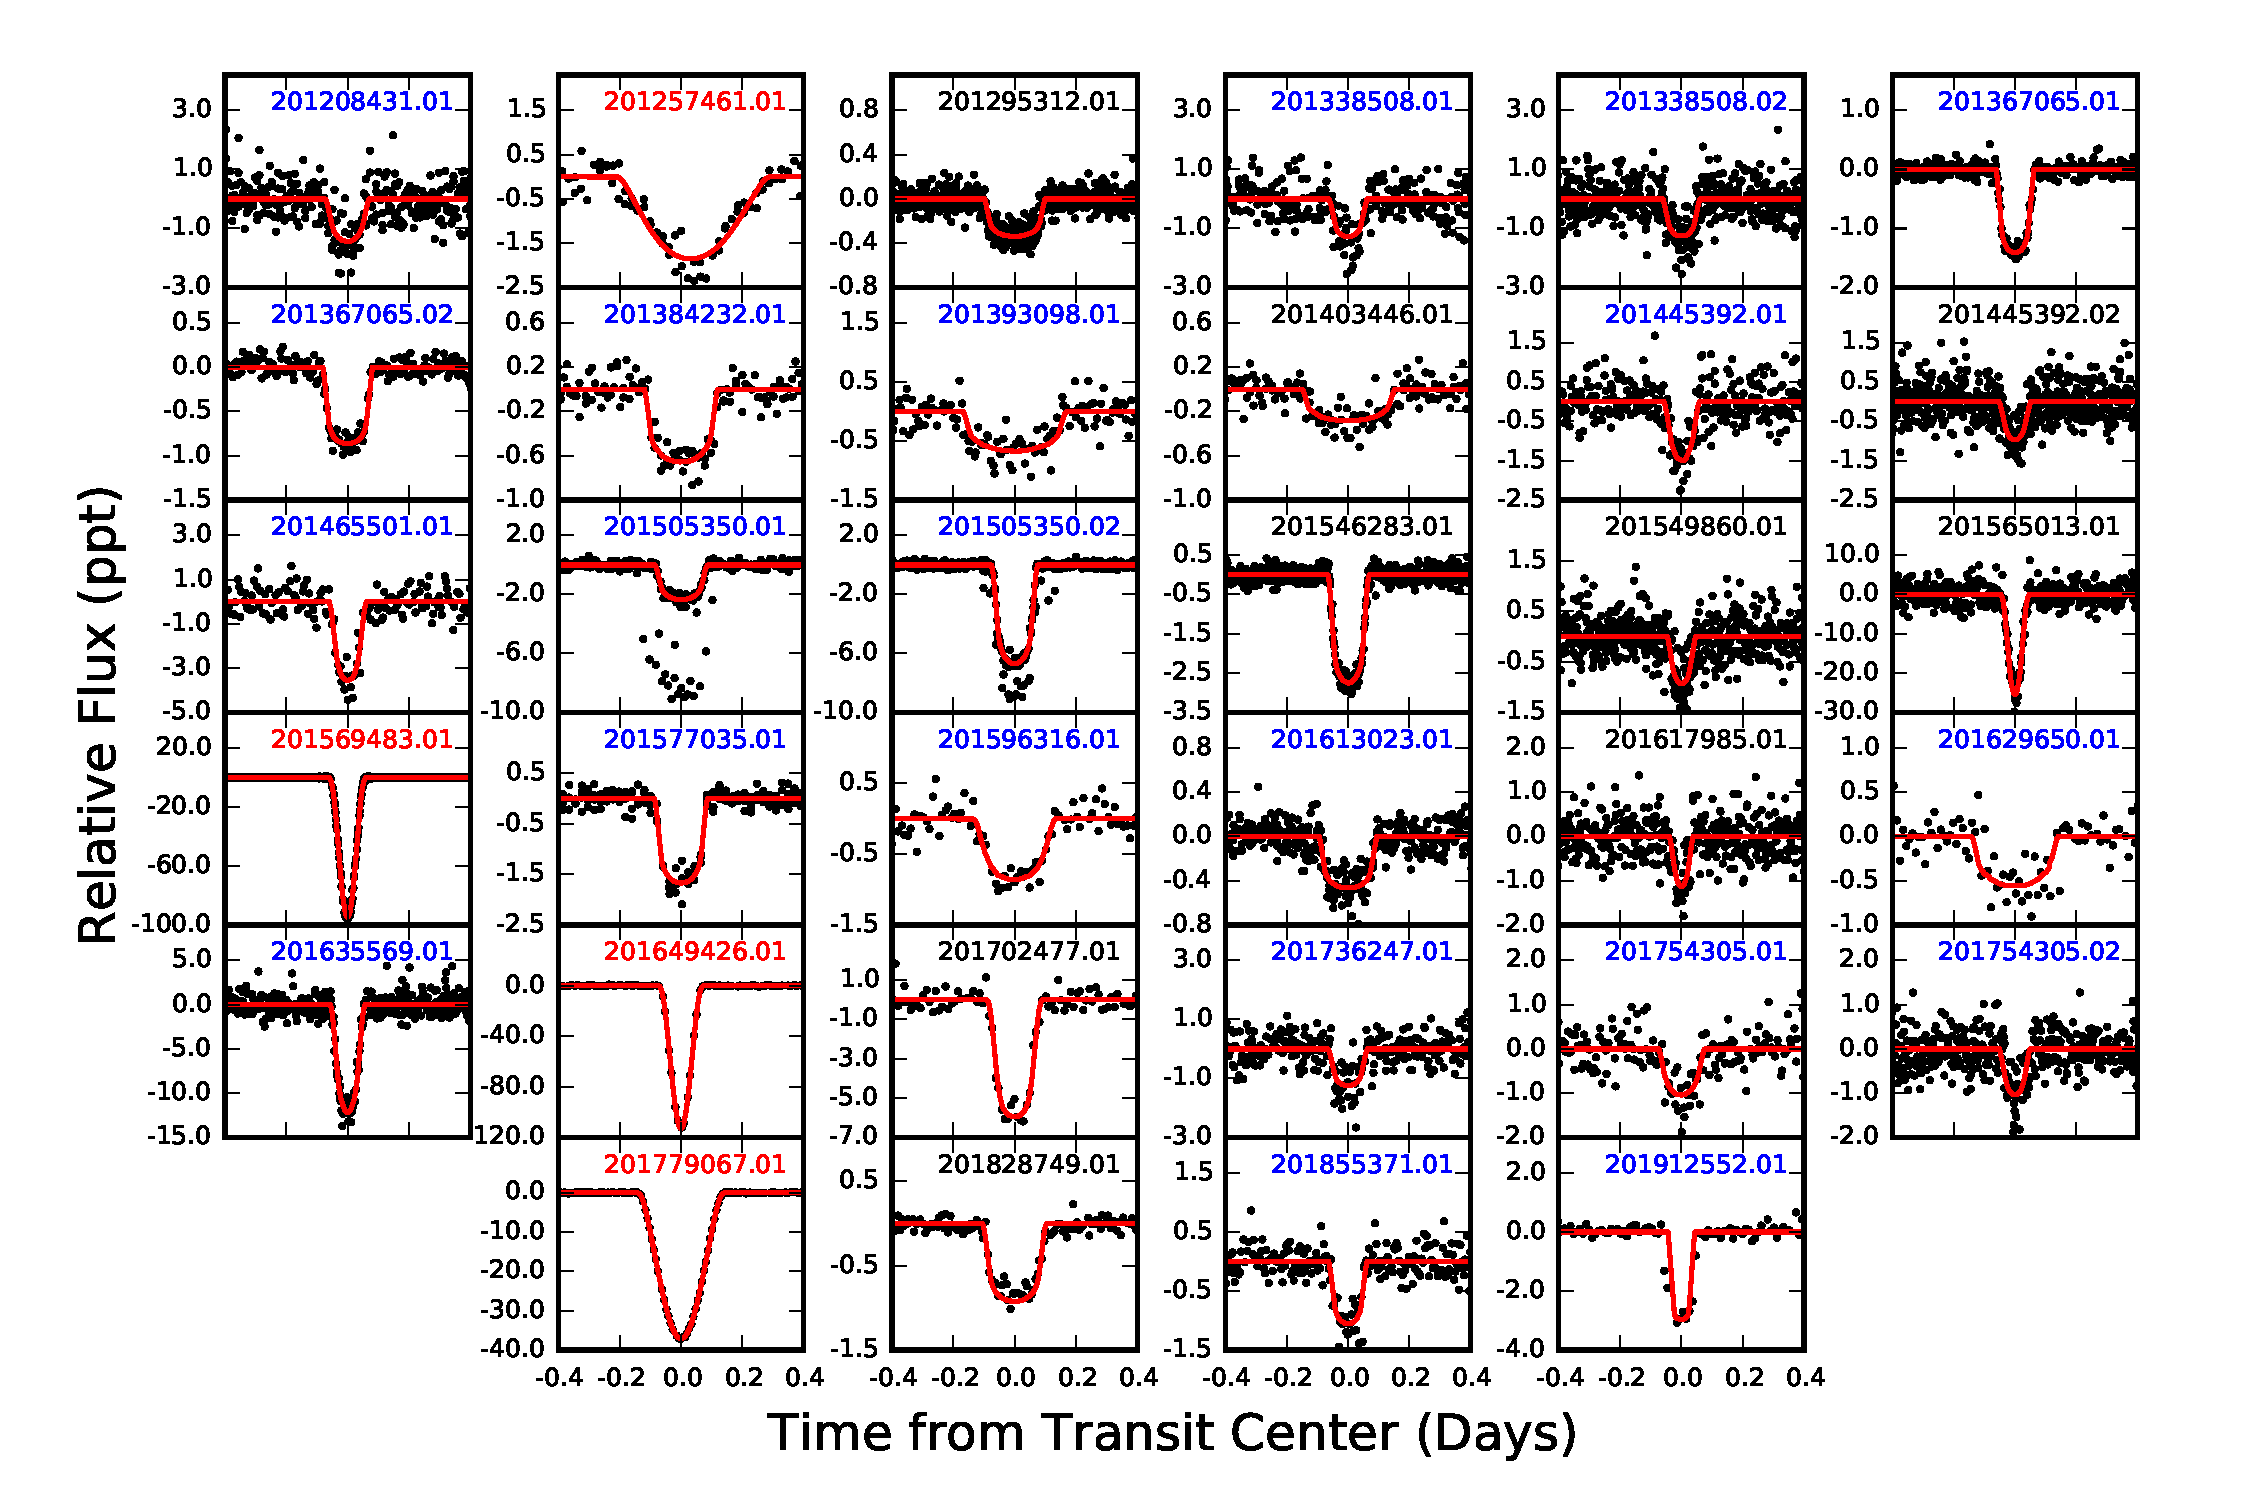
\includegraphics[width=1.0\textwidth]{chapter7/f2.pdf}}
\caption[Phase-folded \KT\ photometry for all planet candidates analyzed in
this chapter]{Phase-folded \KT\ photometry for all planet candidates analyzed in
this chapter.
Each is the product of a fiducial noise model, in which the median systematic
has been removed for illustrative purposes.
The systems which we validate as transiting planets are labeled in
blue.
The systems which we confirm as false positive events are labeled in red.
The systems which we leave as candidates are labeled in black.
Red curves outline the median transit model for each candidate system.
}
\label{fig:transits}
\end{figure}

\subsection{Secondary Eclipse Observations}
\label{sec:sec}
One of the definitive signatures of a false positive binary star system masquerading
as a transiting planet is the presence of a secondary eclipse. While a nondetection of a secondary
does not exclude the possibility of a binary system (the orbit may be eccentric,
or the companion too faint for a secondary eclipse to be detectable in the noise),
such a nondectection reduces the probability of each of the eclipsing binary false
positive scenarios.

To attempt to eliminate each eclipsing binary scenario, we first search each \KT\
light curve to determine which secondary eclipse signals are not allowed by the data.
We mask the transit signal of the planet in question and search for the most significant
signal at the same period.
Such a scheme does not assume circular orbits: we return the most significant signal
at any phase, not only at the midpoint between consecutive transits.

We report these maximum allowable secondary eclipse depths in Table 7.5.
These values are used by \texttt{vespa} as limits on the allowable secondary eclipse.
Any models that cause a larger event, such as a background eclipsing binary
consisting of two equal-mass stars in a circular orbit, can be excluded by the data.
We note that with the exception of K2-19c, all systems with a maximum
eclipse depth of at least one part per thousand have FPPs of 0.866 or larger.
The exception, K2-19, is a two-planet system with the two planets near a 3:2 period
commensurability, so in this case the ``secondary'' is actually the transits of the
other planet.


\subsection{Adaptive Optics Imaging}
\label{sec:AO}

We obtained high resolution images of seven stars with the
Palomar High Angular Resolution Observer (PHARO) infrared detector
\citep{Hayward01} behind the PALM3000 adaptive optics system \citep{Dekany13}
at the Palomar 5.1-meter Hale telescope on the nights of 2015 February 3 and 4 UT.
Sky conditions were mostly clear with light cirrus and $\approx$1.0--1.3 arcsecond seeing
on both nights.
We used the smallest plate scale of 25~mas pix$^{-1}$ which resulted
in a field of view of 25.6$\times$25.6 arcsec across the 1024$^{2}$ pix$^{2}$ array.
All observations were obtained with the 32x pupil sampling mode, resulting in Strehl ratios
of $\approx$20--30\% in $K_S$ for our $V$=11--13~mag targets as measured by the Strehl
monitor at the telescope in real time.
We obtained unsaturated dithered frames of each target in $K_S$-band with typical
integration times of 2--10~s.
Except for EPIC~201828749 and EPIC~201546283, which had nearby candidate
binary companions, we also
acquired deep saturated images (5--10 frames at 60 sec each)
to search for fainter companions.

Images were registered and contrast curves were generated following \citet{Bowler15a}.
For the saturated data, the star's position in each image was found by masking the
saturated region and fitting a 2D bivariate Gaussian to the PSF wings.
Contrast
curves for the median-combined image are calibrated using the unsaturated frames.
The typical sensitivity is 6.5--7.5~mag at 1$''$.
The images were astrometrically calibrated using dithered observations of the
Trapezium cluster centered
on $\theta$$^1$~Ori~C taken on 2015 Feb 3 UT.
Based on the reference astrometry for pairs of stars in the field from
\citet{McCaughrean94}, we measure a plate scale of 25.2~$\pm$~0.4~mas pix$^{-1}$
and north orientation of --0.2~$\pm$~0.3$^{\circ}$.
Since this latter value is consistent with being aligned with
the detector columns, we adopt a value of 0.0~$\pm$~0.3$^{\circ}$ for this work.
Relative photometry of nearby stars is carried out using aperture photometry with
an aperture radius of 12~pix (0.3 arcsec).
For EPIC~201828749, we also acquired $J$- and $H$-band images.
Astrometry and photometry is derived separately for each image, and the mean and standard deviation
of these measurements is adopted for our final values listed in Table~7.4.


Images for all systems AO data was obtained for is shown in Figure~\ref{Fig:AO},
while contrast curves showing the $5\sigma$ limits for detection
as a function of orbital separation are given in Figure~\ref{Fig:CC}.

\begin{figure}[htbp]
\centerline{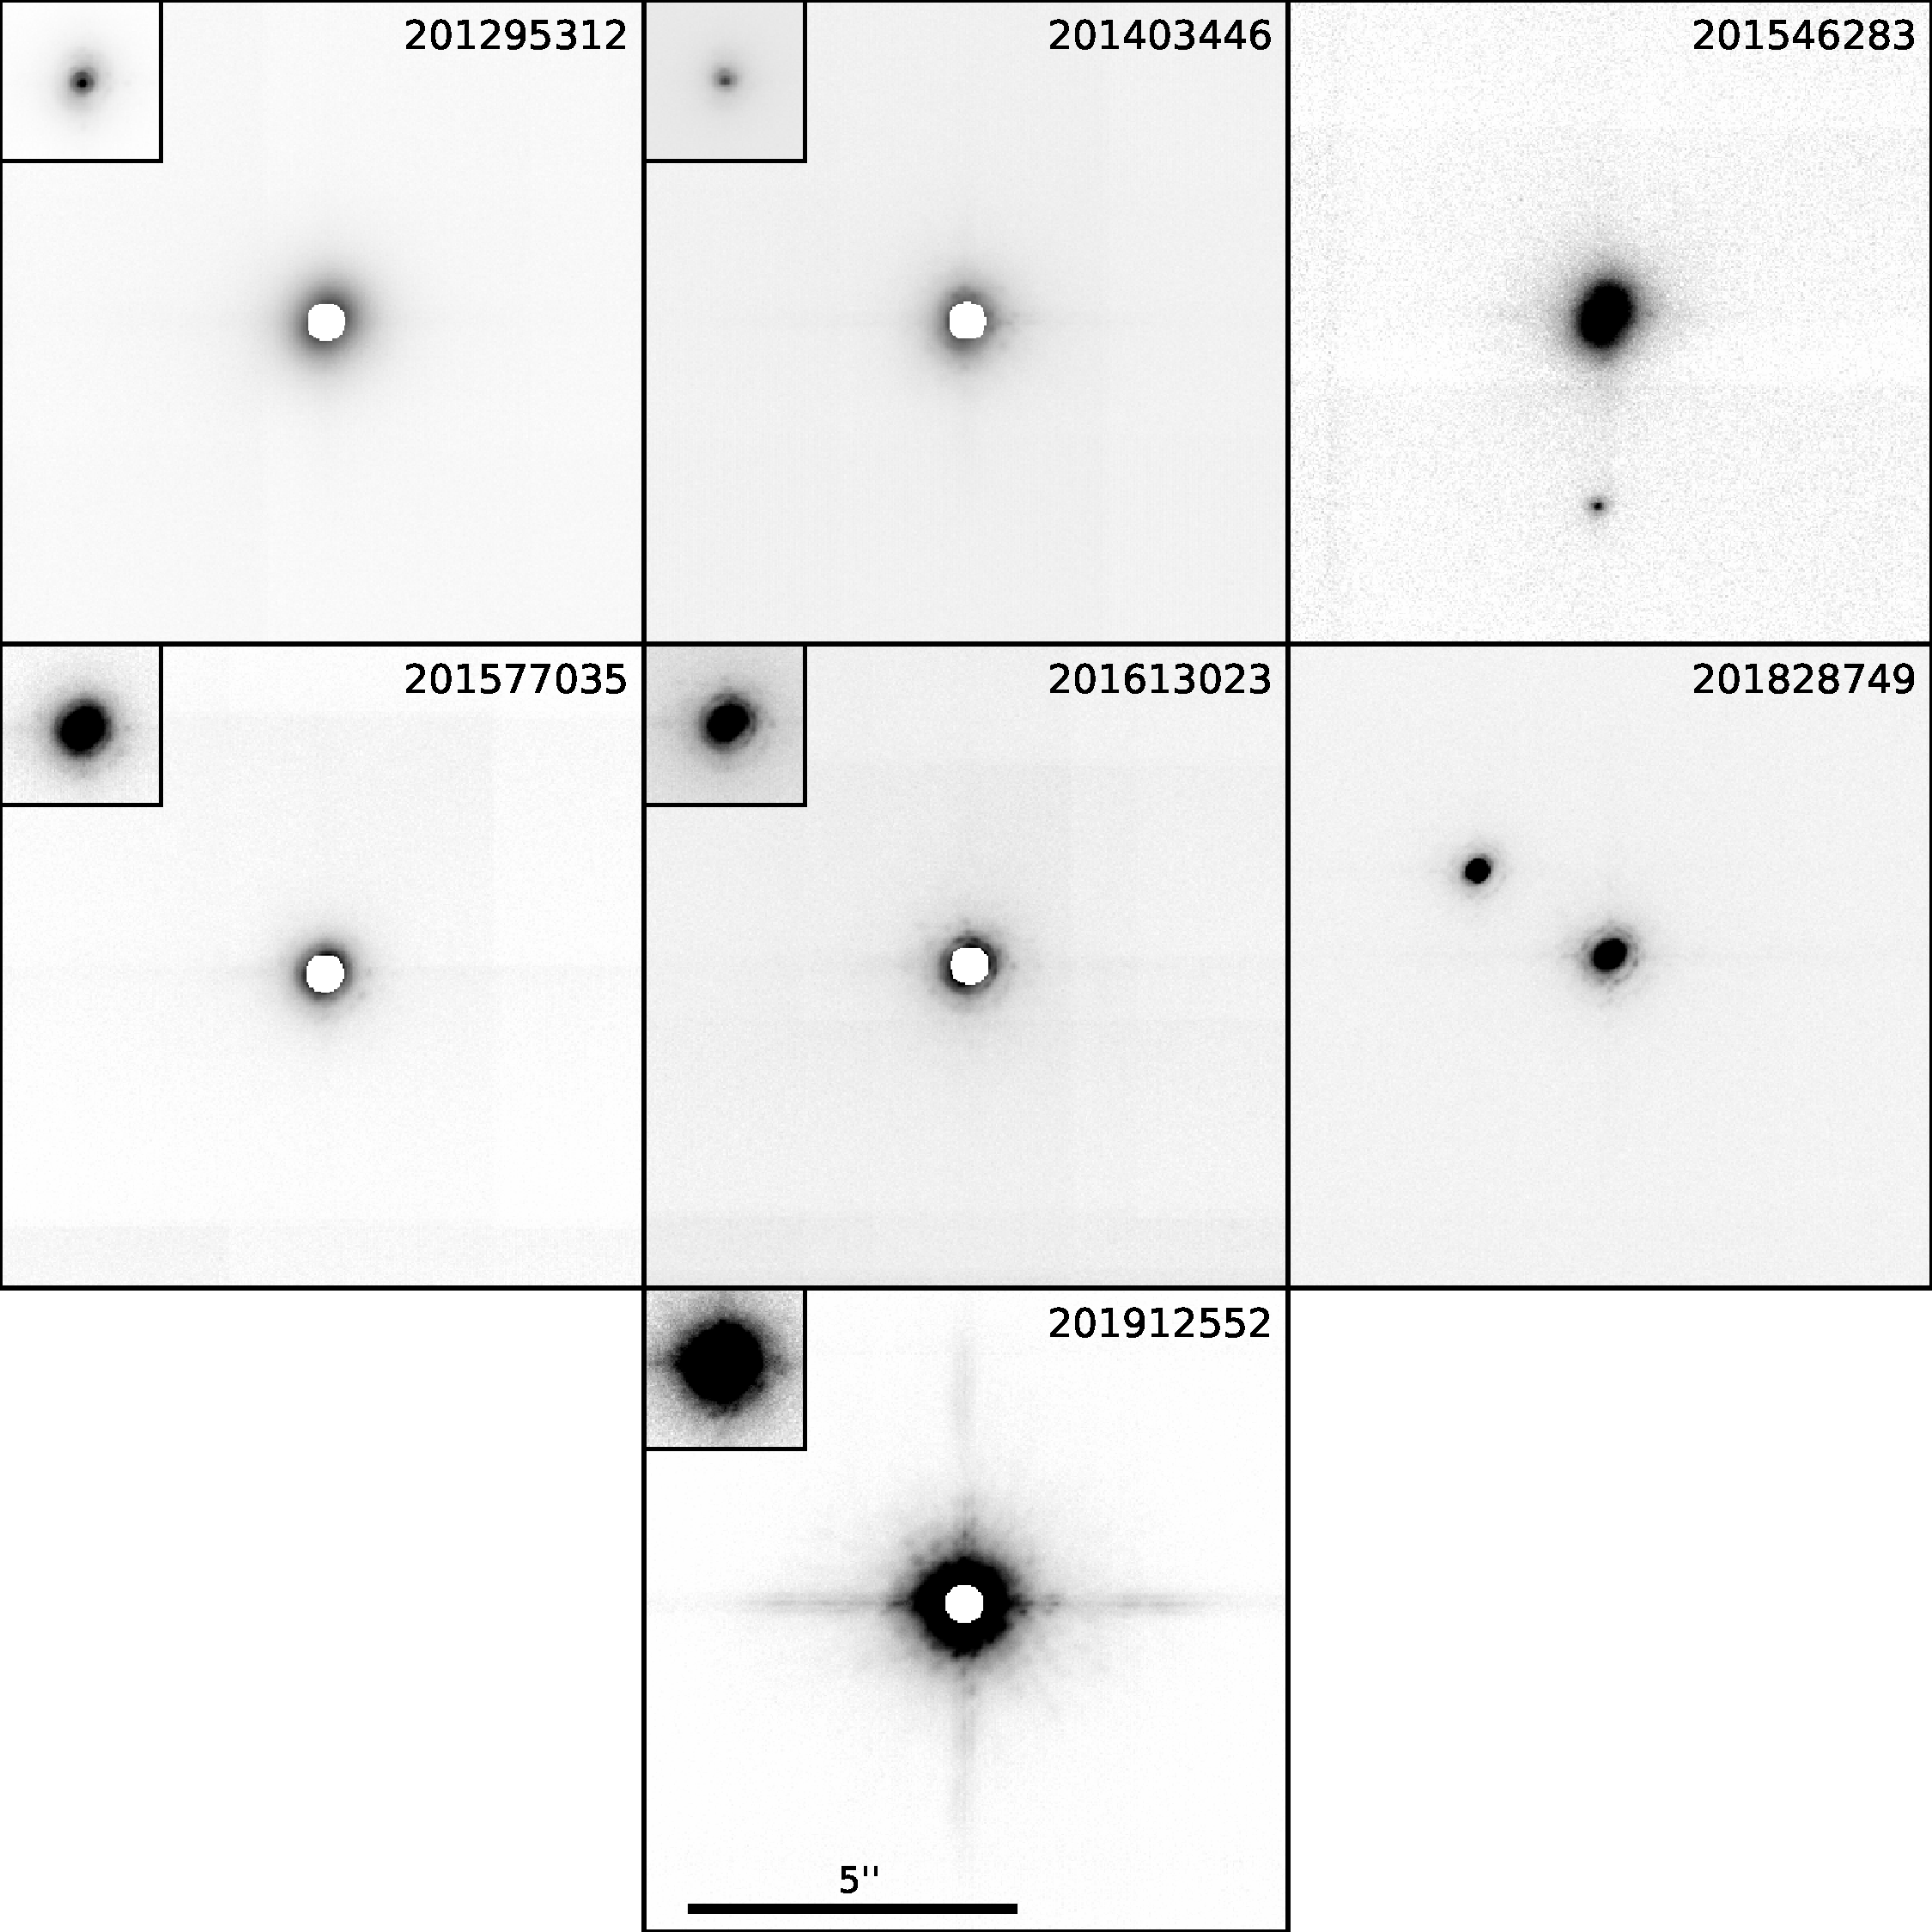
\includegraphics[width=1.0\textwidth]{chapter7/f3.pdf}}
\caption[Adaptive optics images for the seven stars observed with high-contrast imaging]{Adaptive optics images for the seven stars observed with high-contrast imaging.
The main frame for each single system shows the deep, saturated image.
The inset for each single system shows a shallower, unsaturated image to better
identify companions at close projected orbital separations.
For the two systems with imaged companions, EPIC 201546283 and
EPIC 201828749,
only unsaturated frames are collected.
The pixel scale is $0.0252$ arcsec per pixel.
Each subplot is a square 400 pixels on a side and
each inset is a square 100 pixels on a side.
All subplots, including insets, are plotted on the same scale.}
\label{Fig:AO}
\end{figure}

\begin{figure}[htbp]
\centerline{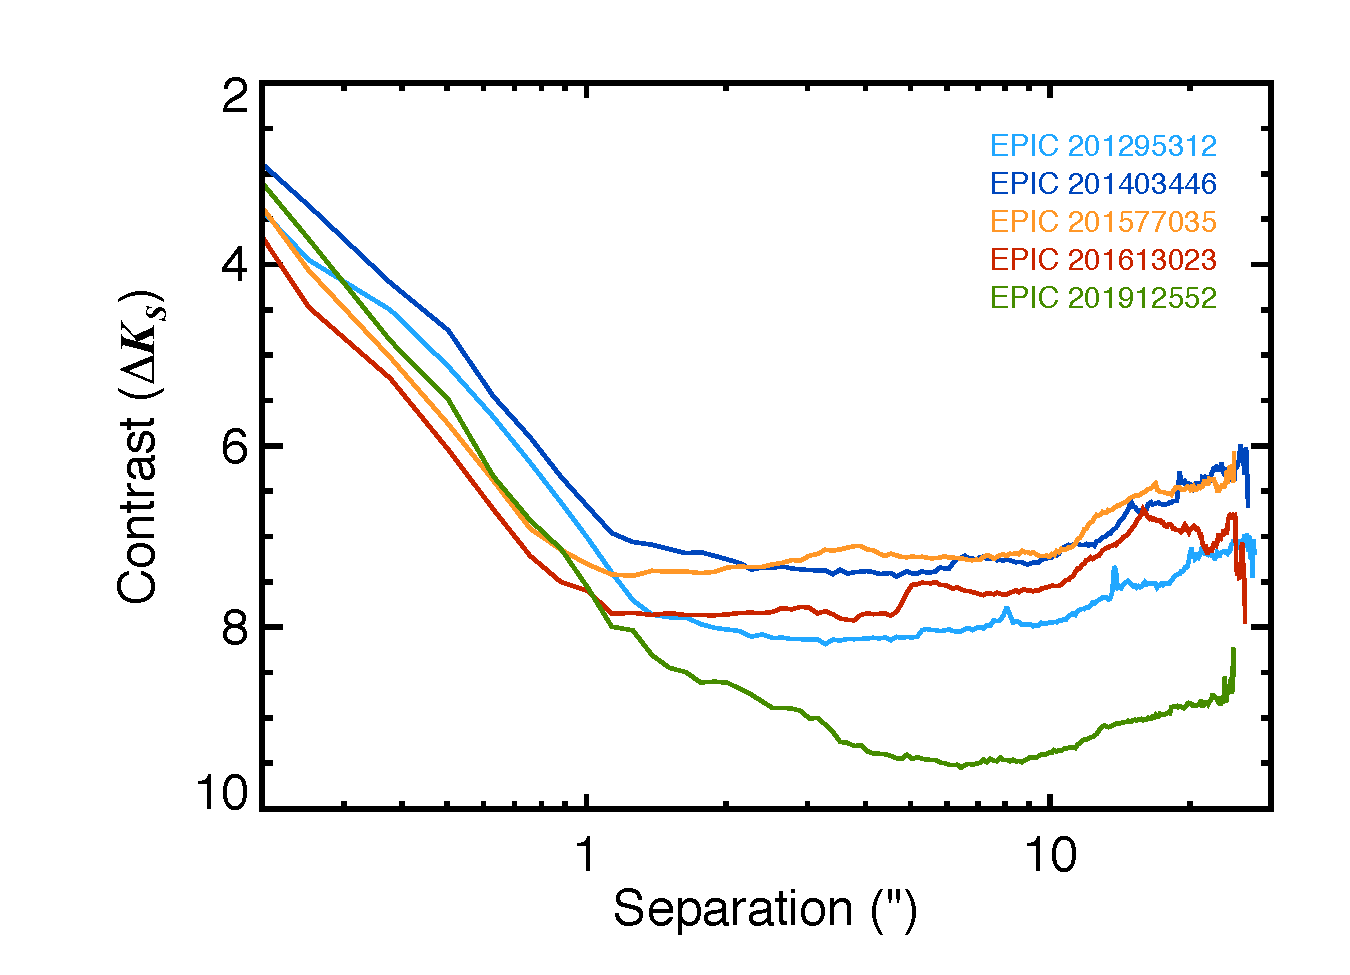
\includegraphics[width=0.75\textwidth]{chapter7/f4.pdf}}
\caption[$5\sigma$ contrast curves for all systems with AO nondetections]{$5\sigma$ contrast curves for all systems with AO nondetections.
For all systems, we can exclude the possibility that a companion at a given $\Delta K_S$
exists.
From our known transit depths, we can then rule out significant parameter space in which
an eclipsing binary could reside and mimic a transit signal.}
\label{Fig:CC}
\end{figure}



\subsection{Known Background Stars}
\label{sec:background}
The PHARO AO system has a field of view of 25 arcseconds.
Each \KT\ pixel is a square, $3.98$ arcsec on a side.
A background eclipsing binary within a few \KT\ pixels of our target
stars could mimic a transit signal inside our aperture while evading detection
by PHARO.
Such wide eclipsing binaries should appear in seeing-limited ground-based
surveys.

To investigate the possibility that such wide companions exist,
we query the ninth data release of the Sloan Digital Sky Survey
\citep[SDSS DR9,][]{Ahn12}.
For each target, from the depth of the observed transit we determine how
bright a background object must be to cause the event if the background
object were an equal mass totally-eclipsing binary.
We then search for all stars within 25 arcsec that are within this brightness
limit relative to the candidate host star.
All apertures we use in our \KT\ analysis are smaller than 20 arcsec so this
search should encompass the region where possible background
contaminants could reside.
Of the 31 stars in our sample, eleven have such a companion, plus one
detected in AO imaging.



Unlike the original \kep\ field, the field for \KT\ \Ci\ is
well out of the Galactic plane, so the rate of giant, distant background
stars is significantly lower.
We include all potential contaminants in Table 7.4.
We validate or eliminate each of these as a possibility based on the transit shape.
For example, the events near EPIC 201546283 could only be caused by a
background binary if the background object was a completely-eclipsing system
(so that the eclipse depth was $50\%$).
In this case, the transit would be V-shaped.
Since it is not, the background object likely does not cause
the transit event.


In Table 7.4, the ``maximum depth'' column represents
the maximum observed ``transit'' depth if the transit were actually caused
by a total eclipse of the hypothetical background binary system, inducing
a 50\% flux decrement in the background star's apparent brightness.

The photometric apertures used to detect these candidates range in radius from
$10.0$ to $19.9$ arcsec.  In order to be a plausible contaminant,
any companion star must
be either within this aperture or just outside but bright
enough for signficant flux to leak in.
Evaluating each of the systems listed in Table 7.4, we judge that we cannot yet
rule out contamination as a potential source of the transit signal for four
candidates: 201295312.01, 201403446.01, 201546283.01, and 201828749.01.
Despite receiving
low FPP scores from \texttt{vespa}, we list these systems as candidates in
Table 7.5, rather than planets.  Further updates to the \texttt{vespa} code
will allow consideration of ``specific'' false positive scenarios; that is,
scenarios that correspond to actually detected stars such as these, rather than
hypothetical background or bound companions.

The candidates with identified companions that we judge to not be plausible
sources of potential contamination are the following:
\begin{itemize}


\item K2-13b (201629650.01)--- The companion to this star is $17.3$ arcsec from
the EPIC target.  As this is outside the aperture
(radius $15.9$ arcsec) and the background star is not particularly bright,
we rule out contamination for this system.

\item 201702477.01--- The companion to this star is $12.15$ arcsec from the
EPIC target, and the aperture size is $10.0$ arcsec.  In addition,
the maximum depth in this system is almost identical to the transit depth.
For these two reasons we rule out contamination in this case.

\end{itemize}

SDSS is 95\% complete at $r=22.2$ mag and the telescope has a point
spread function of $1.4$ arcsec.
For the purposes of the \texttt{vespa} calculation, we thus
treat nondetection in SDSS data as providing a contrast curve at
wide separations
down to a limiting magnitude of $r=22.2$ mag.

\subsection{Archival Imaging}

For the stars with AO nondetections, there is still the
possibility that a background binary could be positioned
directly behind the target star, evading detection.
The probability is small, given the $0.1$ arcsec diffraction limit
of the Hale Telescope at $2$ $\mu$m, but nonzero.
While the \texttt{vespa} calculations quantify this probability for
this to occur, we can also rule out the possibility of such
chance alignments, down to a certain contrast, with archival imaging data.

Five of the stars in our sample have proper motions larger than 50 mas
yr${-1}$, so they have moved across the sky by $\gtrsim 2.5$ arcsec since
they were imaged during the first Palomar Observatory Sky Survey (POSS) in the
1950s.
To rule out background companions, we download data from the POSS I
and II surveys, which imaged these targets in 1952-1955 and 1989-1998,
respectively.
We also download data from the Sloan Digital Sky Survey, which imaged
these fields between 2000 and 2009.
As shown in Figure~\ref{fig:archival}, we do not detect any background
targets at the present-day location of any of these stars in any of these
images.



\begin{figure}[htbp]
\centerline{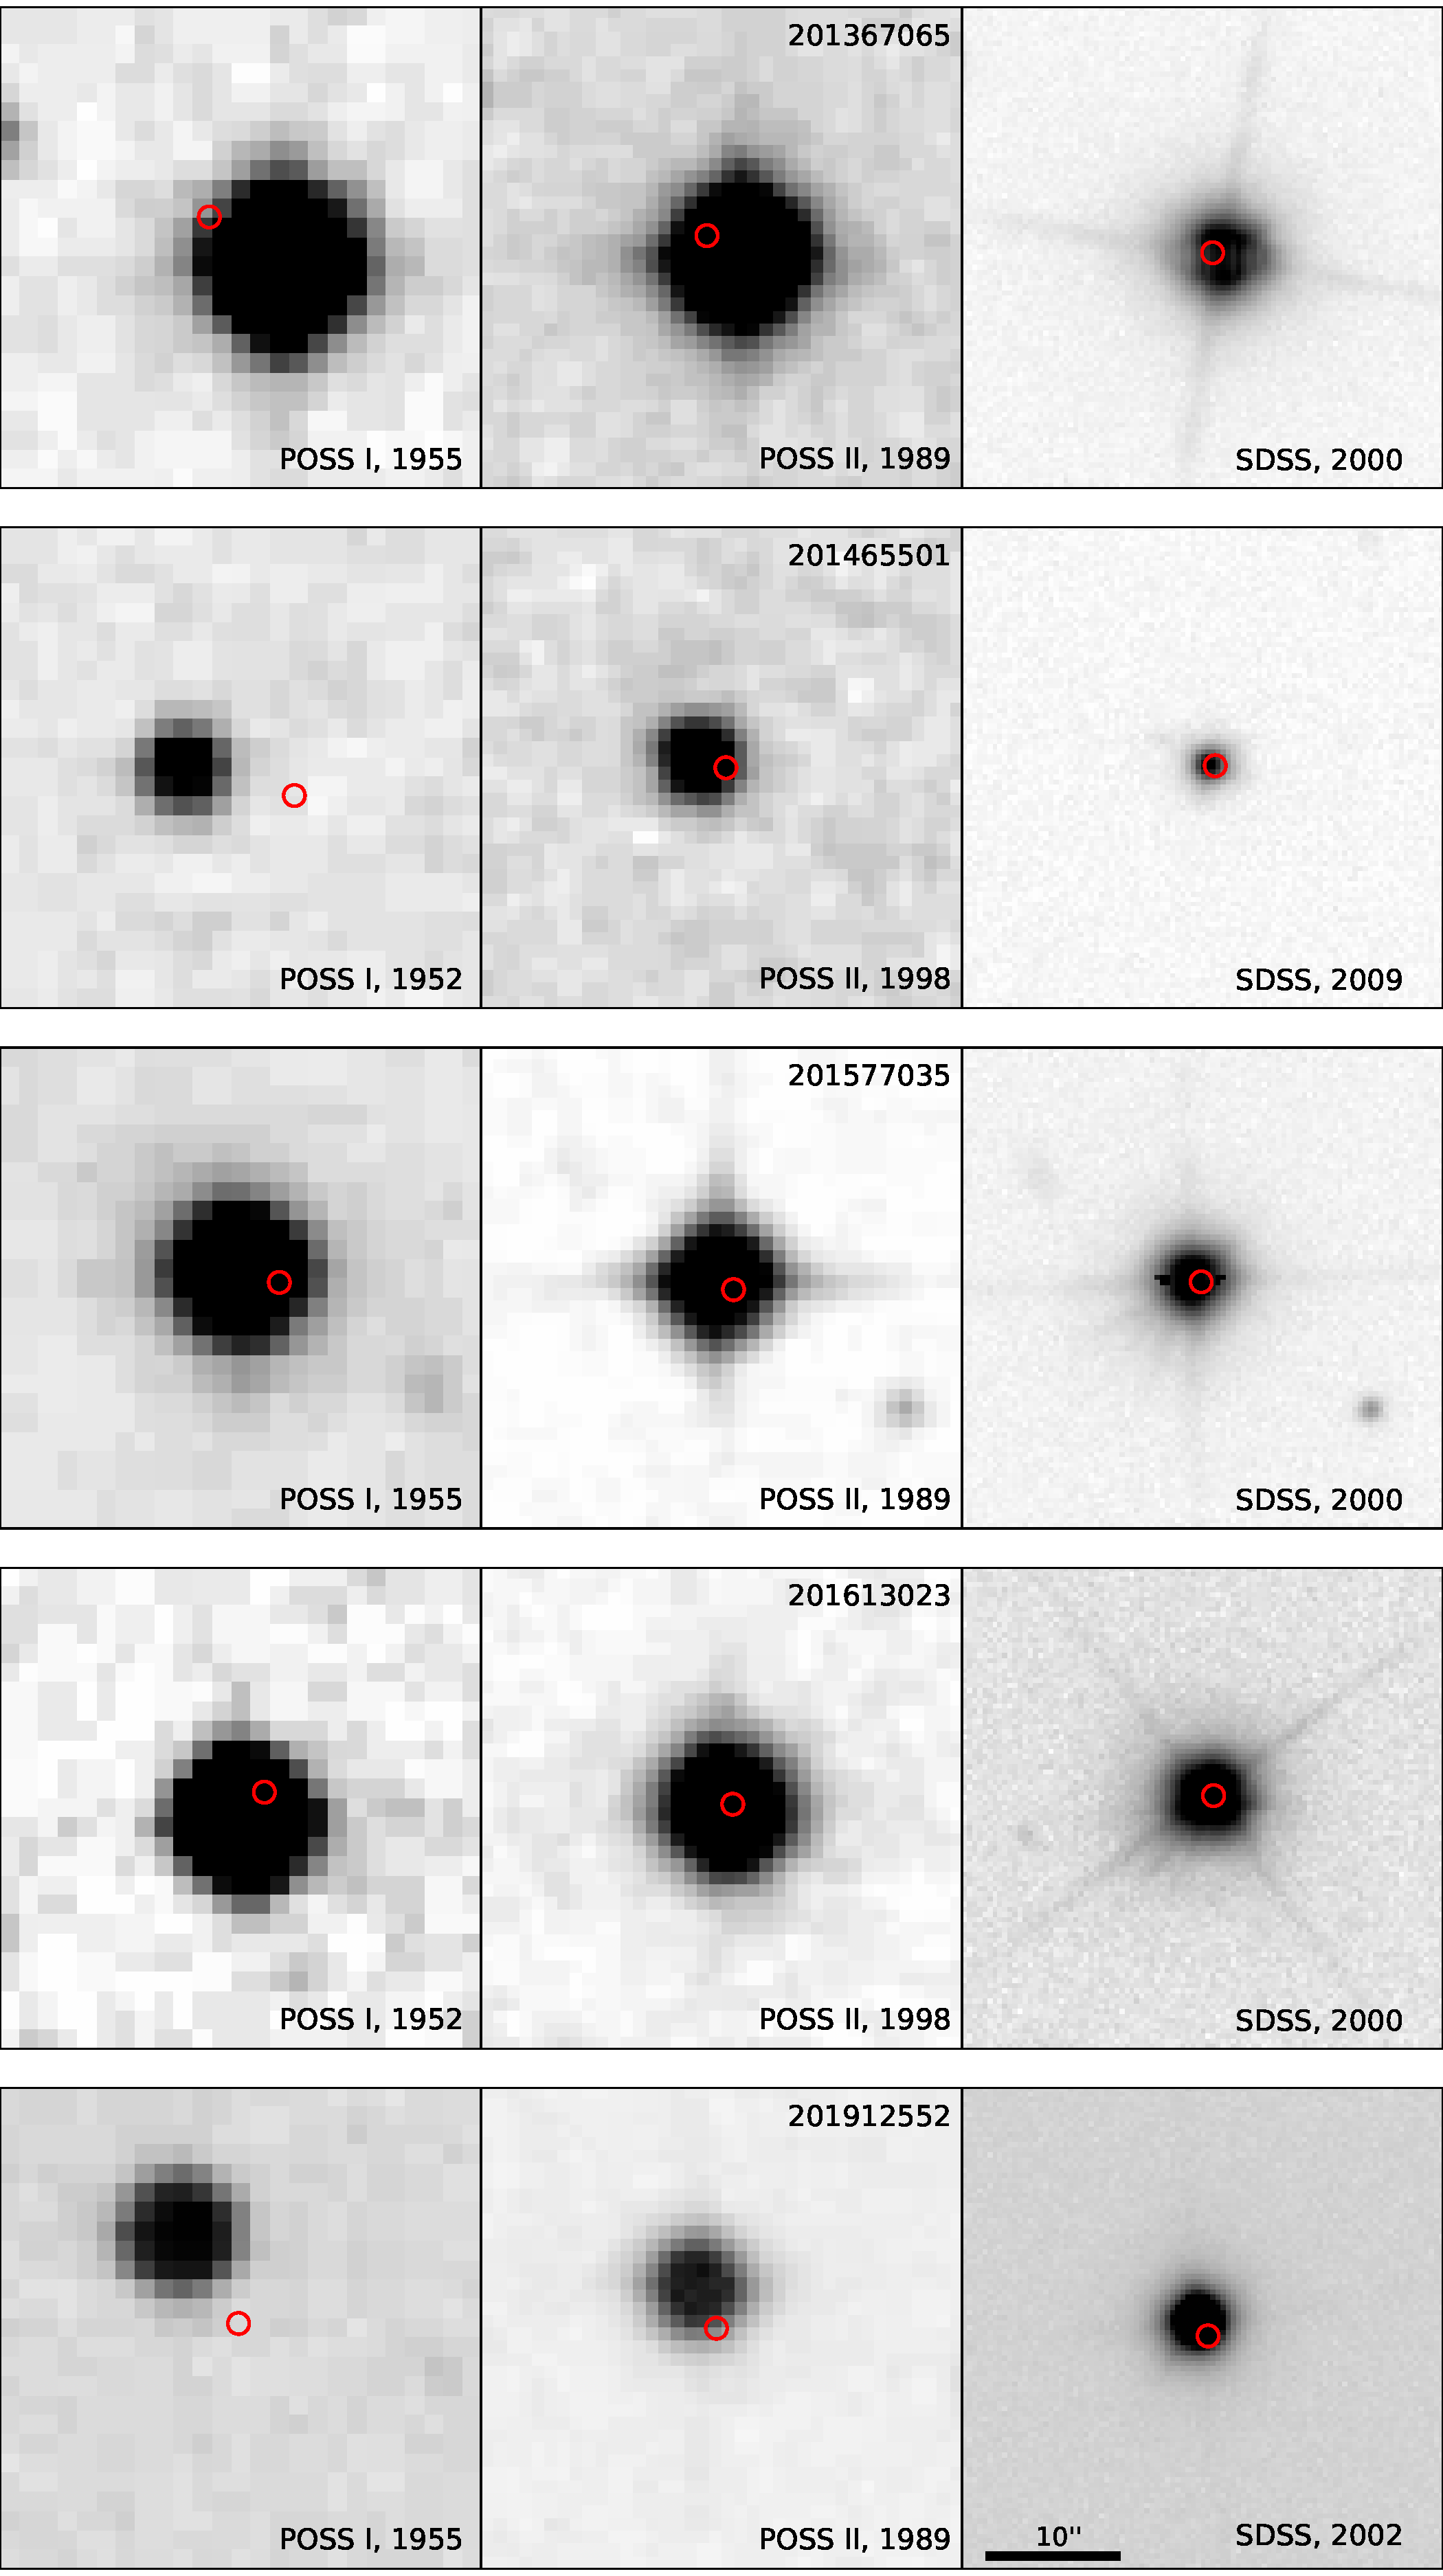
\includegraphics[width=0.65\textwidth]{chapter7/f5.pdf}}
\caption[Archival maging for the five highest proper motion targets in our sample]{Archival maging for the five highest proper motion targets in our sample.
In all cases, there are no background
objects directly behind the present day location of the target (red circle) that could be missed
by the AO observations. Modern SDSS imaging can also rule out wide companions
that may have been missed at wide separations, beyond the AO field of view, such as the
companion which can be seen in the images of K2-10.
All figures are aligned such that north is up and east to the left.
All subplots are on the same scale.}
\label{fig:archival}
\end{figure}


For this target, we can extend our contrast curves to zero
present-day orbital separation and rule out the possibility that
these transit events are caused by a background eclipsing binary.
By combining present-day seeing-limited photometric survey data,
adaptive optics imaging, and archival photometry, the only stellar companions
we would not detect would be those that are gravitationally bound to the target
star and positioned in their orbits so that their projected separation is
smaller than the diffraction limit of the Hale Telescope.
Such an alignment would require the orbital inclination of the binary to be
nearly $90^\circ$ and the phase $\varpi + \theta \approx \pi/2$ or $3\pi/2$.
While we cannot fully rule out this possibility, the \texttt{vespa}
calculations confirm that its probability is negligibly small.




\subsection{TRES Radial Velocities}

We observed K2-18 on 2015 February 04 and 25 UT
with the Tillinghast Reflector Echelle
Spectrograph (TRES) on the 1.5 m Tillinghast Reflector at the Fred L.
Whipple Observatory.
These dates were chosen to be near the times of largest RV variations,
corresponding to phases of 0.72 and 0.32 relative to the time
of transit.
The spectra were taken with a resolving power of $R=44,000$ and
integration times ranging from 2800 to 3600 seconds, resulting in
signal-to-noise ratios between 17 and 29 per resolution element.

The spectra were extracted as described in \citet{Buchhave10}.
The relative RVs were derived by cross-correlating the spectra against the
strongest observed spectrum (in this case, the first) over the wavelength
range 4700 - 6800 Angstroms.
We selected 19 echelle orders in the analysis, being careful to reject
orders with telluric absorption lines, fringing in the far red and those
with very low SNR in the blue.

The two observed spectra have RVs that differ by $47 \pm 42$ m s$^{-1}$.
If the RVs were caused by a stellar companion, the RV shift between these
observations would be on the order of km s$^{-1}$.
Therefore, we can rule out any stellar-mass companions that would be able
to create this transit signal.




\section{Potentially Interesting Systems}
\subsection{A Mini-Neptune with Earthlike Insolation}

The planet orbiting K2-18 may be an interesting target for
atmospheric studies of transiting exoplanets.

By combining archival and modern seeing-limited data with adaptive optics
imaging, we can exclude the possibility these transit events are caused by
a background eclipsing binary.
The apparent transits must be caused by an object co-moving with K2-18;
radial velocities eliminate the possibility the companion is nonplanetary.
Therefore, we confirm the planetary nature of this system.

This star is an M2.8 dwarf at a distance of $34\pm4$ pc.
Of our planet candidate hosts, only K2-3 \citep[originally
discovered by][]{Crossfield15} is brighter in $K$-band.
This star is only 0.1 magnitudes fainter in $K$ than GJ\,1214
\citep{Charbonneau09}.
Due to the relative brightness of the host star, this target is likely
to become a prime target for atmospheric characterization studies
and is ideal as a target for future space-based missions such as
\textit{JWST}.

The planet is slightly smaller than GJ\,1214b, but unlike that planet,
K2-18b is not highly irradiated.
Instead, it is at a reduced semimajor axis \ars$ = 83.8 \pm 9.0$.
Its equilibrium temperature is then, assuming zero albedo, $T_{eq} = 272 \pm 15$
K, meaning its bulk insolation is $128 \pm 28$ percent that of the Earth's.
Although the planet is likely too large to be rocky \citep{Rogers14},
its atmosphere is likely to be the focus of many future observations, providing
a cool analogue to the highly irradiated planets of a similar size found by
\kep.


\subsection{Other Sources of False Positives}
\label{sec:systematics}

The method of \paperit\ assumes that all variability in the light curves are
caused by either the motion of \KT, in which case the variability is shared
by all stars, or transits of planets, in which case the variability is intrinsic
to only one star.
This assumption breaks down for extremely spotted stars where the
astrophysical variability is larger than the instrumental
magnitude.
In that regime, the starspot modulations can be incorrectly fit by the
systematic model, causing spurious transits to appear.
This appears to be the case with EPIC 201929294, which has
coherent starspots that appear to have the same rotation period as the
transit period reported previously.
Because the starspots are so periodic and coherent, these spurious
transits were falsely identified as a planet candidate; we consider that
system a false positive in this work.

The candidate object possibly orbiting EPIC 201555883 has a period,
time of transit, and transit duration consistent with EPIC 201569483.
Such effects are not uncommon in \kep\ data.
\citet{Coughlin14} identify 685 KOIs as false
positives and outline four physical reasons why these anomalies may occur.
EPIC 201555883 is a unique case in that it does not appear to fall under any
of these cases. It falls on module 23, while EPIC 201569483 is on module 8,
neither 180 degrees away from nor on the same column as this candidate.
Moreover, there is not any evidence of a mechanism that could cause a third
star to induce both the appearance of a $7\%$ eclipse on one module and an
additional anomalous transit event on a different module.
Instead, this candidate could be a false positive caused by a different
systematic mechanism.

\paperit\ modeled the systematic effects in the \KT\ light curves using a
linear combination of ``eigen light curves'' generated empirically by running
a principle component analysis on the light curves of every star.
This means that the training set includes the light curves for variable stars,
eclipsing binaries, and even transiting planets.
Again, this star has significant variability caused by starspots.
In this case, the fitting procedure tries to account for stellar variability using
the eigen light curves.
This overfit gives undue weight to eigen light curves that include the transits
of EPIC 201569483, causing this spurious transit to occur.
Again, we consider this system to be a false positive.
As stated in \textsection 3, by including an empirical Gaussian
prior on the weights for the eigen light curves in the linear systematics model,
the signals observed on EPIC 201555883 and 201929294 are mitigated, suggesting
such a scheme should be employed in searching for planet candidates in future
campaigns.

The problem of over-fitting stellar variability using eigen light curves can also be
solved by adding a stellar activity model to our fitting procedure.
In this case, the spacecraft motion could be fit simultaneously with a model
of starspot modulation, astroseismic oscillations, and planet transits.
Such a model is currently under development (Angus et al. \textit{in prep}).


\subsection{Multiple Planet Systems}
Five of the systems reported by \paperit\ have more than one transiting
candidate.
One of these is K2-3, a three-planet system originally announced by
\citet{Crossfield15}.
Another of these is K2-19 \citep{Armstrong15b}, a two-planet system with the
orbital periods of the two planets near a 3:2 period commensurability.
The remaining three are all representative of the multiple-planet systems observed by
\kep\ \citep{Lissauer11b, Fabrycky14}.
Two of the systems are near a period commensurability and all three consist of
mini-Neptune sized planets.



We do not detect any significant transit timing variations (TTVs) in any of these systems from
the \KT\ data alone.
K2-5 would be expected to have a TTV period of 117 days, but
is likely too far from commensurability to have an observable TTV signal.
K2-8 is expected to have a TTV period of 234 days, so this system may be a candidate
for additional follow-up to constrain the system masses dynamically.
The transiting planets orbiting K2-16 are near a 5:2 period commensurability.
There is no evidence from \kep\ of an abundance of planets near this period ratio, and so this
may be coincidence.
Follow-up observations may be warranted to search for an additional planet in this system
forming a resonant chain, similar to those observed around other stars \citep[e.g.][]{Swift13,
Campante15}.

\subsection{Systems Orbiting Bright Stars}

One of the primary goals of \KT\ is the detection of transiting planets around bright stars that
can be followed up from the ground or with future space-based observatories such as JWST
\citep{Howell14}.
Of our sample, two systems orbit stars with $K < 9$ mag: K2-3 \citep{Crossfield15} and
K2-18.
An additional planet candidate may orbit EPIC 201828749, a star with $K = 9.93 \pm 0.03$ mag.
These targets are ideal for ground-based followup and may be useful targets for Spitzer and
JWST to probe planetary atmospheres.

\section{Results and Discussion}

We have presented stellar parameters for all planet candidates systems identified by
\paperit.
We statistically validate \Nvalidated\ of the 36 candidates as bona fide planets, and we
identify \Nfp\ as false positives, including two systematic false alarms.
Of the planets, 4 have been previously validated in other works, while \Nvalnew\ are
validated here for the first time.
The systems not validated as planets or false positives remain as planet candidates.

Enabling much of this analysis are two new publicly available Python packages:
\texttt{isochrones}\footnote{\url{http://github.com/timothydmorton/isochrones}},
which we use to infer posteriors on physical stellar properties based
on fitting theoretical stellar models to observed data; and \texttt{vespa}\footnote{
\url{http://github.com/timothydmorton/vespa}}, a
new implementation of the \citet{Morton12} transit false positive analysis scheme.
Both of these packages will continue to be useful in future analysis of transit candidates
where comprehensive follow-up observations may be unavailable.

The \texttt{isochrones} package uses the nested sampling scheme 
\texttt{MULTINEST} to capture the true multimodal nature of the posteriors.
Using an MCMC algorithm instead can cause only one peak in the posterior
distribution to be sampled. 
If the photometry is consistent with both a star on the main sequence and the
subgiant branch, an MCMC technique could cause one of these peaks (likely the
subgiant possibility) to be missed, leading to an underestimation in the likelihood
of subgiant stars and and underestimation of the uncertainties of both the stellar and planetary 
parameters. 


With the exception of one object, all of the stellar parameters are derived from comparing
photometric observations to the Dartmouth stellar evolution models.
As a result, both the stellar and planet parameters are subject to systematic biases induced
by discrepancies between the models and reality.


The planets we confirm in this paper, like the planets found in the original \kep\ mission,
span a wide range of parameter space.
They are at distances ranging from $34$ to $700$ pc, have radii ranging from $1.3$ to
5.3 $R_\oplus$, and orbit with periods ranging from 5.0 to 50.3 days.
Like the original mission, we find significantly more small planets than large planets, as
expected from the radius distributions measured from \kep\
\citep{Howard12, Fressin13, Morton14}.

Unlike the original mission, however, we find that nearly all of our confirmed planets
are around stars less massive than the Sun.
This difference is a result of both the \Ci\ field and the target selection process.
\Ci\ is at a significantly higher Galactic latitude than the original \kep\ mission,
meaning there is a much lower number density of targets at large distances.
As massive stars
at kiloparsec distances are relatively less likely to exist in \Ci\ than near the
Galactic plane, the pool of targets that could be selected for \Ci\ contains a larger
fraction of subsolar stars.

Low-mass stars, particularly M dwarfs, are also a specific focus of the \KT\ mission.
One of the primary goals of the \kep\ mission was to ``determine the abundance of
terrestrial and larger planets in or near the habitable zone of a wide variety of spectral
types of stars'' \citep{Batalha13} However, $\sim70\%$ of Kepler's target stars had
masses within 20\%
of the Sun's, while 70\% of the stars in the Galaxy have less than 50\% the mass of the
Sun \citep{Brown11}.
\KT\ will fulfill the promise of \kep, with the goal of providing a yield of small planets
around bright, small stars to facilitate follow-up measurements \citep{Howell14}.
This is clear from the \KT\ target selection process, with thousands of K and M dwarfs
being selected in each campaign.
Based on these plans, we expect that \KT\ will detect hundreds of planets during its
lifetime, with the majority being mini-Neptunes and super-Earths around stars
less massive than the Sun.






\begin{landscape}
\begin{table}[hbt!]
\tiny
\begin{center}
\begin{tabular}{lccccccccccc}
\hline
EPIC & $B^1$ & $V^1$ & $g^1$ & $r^1$ & $i^1$ & $J^2$ & $H^2$ & $K^2$ & W1$^3$ & W2$^3$ & W3$^3$ \\
\hline
201208431 & $16.23(05)$ & $14.91(03)$ & $15.56(04)$ & $14.29(07)$ & $13.89(12)$ & $12.37(02)$ & $11.75(02)$ & $11.57(02)$ & $11.51(02)$ & $11.55(02)$ & $11.58(20)$   \\
201257461 & $12.82(03)$ & $11.77(01)$ & $12.24(04)$ & $11.49(01)$ & $11.19(02)$ & $9.99(02)$ & $9.48(02)$ & $9.37(02)$ & $9.28(02)$ & $9.37(02)$ & $9.30(04)$ \\
201295312 & $12.78(04)$ & $12.19(12)$ & $12.41(03)$ & $12.08(09)$ & $12.01(21)$ & $11.02(03)$ & $10.70(02)$ & $10.69(02)$ & $10.63(02)$ & $10.69(02)$ & $10.75(12)$ \\
201338508 & $16.30(07)$ & $14.91(03)$ & $15.62(05)$ & $14.33(02)$ & $13.79(05)$ & $12.45(03)$ & $11.76(02)$ & $11.60(02)$ & $11.49(03)$ & $11.49(02)$ & $11.16(13)$ \\
201367065 & $13.52(06)$ & $12.17(01)$ & $12.87(03)$ & $11.58(02)$ & $10.98(17)$ & $9.42(03)$ & $8.80(04)$ & $8.56(02)$ & $8.44(02)$ & $8.42(02)$ & $8.32(02)$ \\
201384232 & $13.30(05)$ & $12.65(04)$ & $12.91(05)$ & $12.48(06)$ & $12.34(07)$ & $11.44(02)$ & $11.09(02)$ & $11.07(02)$ & $11.00(02)$ & $11.05(02)$ & $11.21(16)$ \\
201393098 & $13.90(04)$ & $13.21(03)$ & $13.54(06)$ & $13.02(04)$ & $12.85(05)$ & $11.95(02)$ & $11.63(02)$ & $11.56(02)$ & $11.52(02)$ & $11.57(02)$ & $11.61(21)$ \\
201403446 & $12.48(02)$ & $12.03(02)$ & $12.18(01)$ & $11.94(05)$ & $11.86(04)$ & $11.05(03)$ & $10.76(02)$ & $10.78(02)$ & $10.67(03)$ & $10.71(02)$ & $10.36(07)$ \\
201445392 & $15.73(02)$ & $14.61(03)$ & $15.19(04)$ & $14.29(02)$ & $14.03(07)$ & $12.83(03)$ & $12.32(03)$ & $12.24(03)$ & $12.16(02)$ & $12.21(02)$ & --- \\
201465501 & --- & --- & $16.73(02)$ & $15.18(03)$ & $14.35(15$ & $12.45(02)$ & $11.71(02)$ & $11.49(02)$ & $11.35(02)$ & $11.21(02)$ & $11.35(19)$ \\
201505350 & $13.80(02)$ & $13.00(01)$ & $13.36(02)$ & $12.76(01)$ & $12.57(02)$ & $11.60(02)$ & $11.21(02)$ & $11.16(03)$ & $11.10(02)$ & $11.13(02)$ & $10.95(12)$ \\
201546283 & $13.51(07)$ & $12.64(02)$ & $13.03(02)$ & $12.37(02)$ & $12.17(05)$ & $11.16(02)$ & $10.79(03)$ & $10.70(02)$ & $10.61(02)$ & $10.66(02)$ & $10.53(09)$ \\
201549860 & $15.56(06)$ & $14.37(05)$ & $14.95(07)$ & $13.85(03)$ & $13.45(05)$ & $12.14(02)$ & $11.56(02)$ & $11.42(02)$ & $11.38(02)$ & $11.46(02)$ & $11.60(25)$ \\
201555883 & $16.48(01)$ & $15.43(01)$ & $16.19(10)$ & $15.09(13)$ & $14.55(08)$ & $13.20(02)$ & $12.53(03)$ & $12.43(03)$ & $12.34(02)$ & $12.38(03)$ & --- \\
201565013 & --- & --- & $18.25(01)$ & $16.91(01)$ & $16.34(01)$ & $14.78(04)$ & $14.11(05)$ & $14.08(07)$ & $13.94(03)$ & $13.87(04)$ & --- \\
201569483 & $12.90(08)$ & $12.05(07)$ & $12.44(03)$ & $11.76(08)$ & $11.48(08)$ & $10.39(02)$ & $9.97(03)$ & $9.88(02)$ & $9.82(02)$ & $9.87(02)$ & $9.82(05)$ \\
201577035 & $13.14(11)$ & $12.42(02)$ & $12.70(04)$ & $12.21(03)$ & $12.13(20)$ & $11.06(02)$ & $10.75(02)$ & $10.64(02)$ & $10.64(02)$ & $10.69(02)$ & $10.55(10)$ \\
201596316 & $14.21(01)$ & $13.39(09)$ & $13.78(07)$ & $13.14(12)$ & $12.88(10)$ & $11.87(02)$ & $11.46(02)$ & $11.35(02)$ & $11.29(02)$ & $11.35(02)$ & $10.80(11)$ \\
201613023 & $12.99(09)$ & $12.26(01)$ & $12.56(03)$ & $12.05(03)$ & $11.96(08)$ & $10.98(02)$ & $10.71(02)$ & $10.61(02)$ & $10.58(02)$ & $10.63(02)$ & $10.59(10)$ \\
201617985 & $16.34(02)$ & $14.86(05)$ & $15.62(06)$ & $14.26(08)$ & $13.42(09)$ & $11.72(02)$ & $11.09(04)$ & $10.90(02)$ & $10.73(02)$ & $10.70(02)$ & $10.86(11)$ \\
201629650 & $13.61(03)$ & $12.90(04)$ & $13.20(03)$ & $12.73(01)$ & $12.53(06)$ & $11.57(03)$ & $11.26(02)$ & $11.17(03)$ & $11.14(02)$ & $11.18(02)$ & $10.93(12)$ \\
201635569 & $17.74(16)$ & $16.31(01)$ & $17.02(01)$ & $15.62(01)$ & $14.87(01)$ & $13.42(03)$ & $12.77(02)$ & $12.61(03)$ & $12.52(03)$ & $12.55(03)$ & --- \\
201649426 & $14.57(03)$ & $13.53(01)$ & $14.04(01)$ & $13.18(02)$ & $12.86(06)$ & $11.57(02)$ & $11.07(02)$ & $11.07(02)$ & $10.88(02)$ & $10.91(02)$ & $10.86(12)$ \\
201702477 & $15.27(05)$ & $14.57(04)$ & $14.89(04)$ & $14.40(06)$ & $14.24(03)$ & $13.27(03)$ & $12.88(03)$ & $12.77(03)$ & $12.81(02)$ & $12.84(03)$ & --- \\
201736247 & $15.49(06)$ & $14.66(05)$ & $15.01(04)$ & $14.35(04)$ & $14.14(02)$ & $13.07(02)$ & $12.55(02)$ & $12.49(03)$ & $12.46(02)$ & $12.50(02)$ & --- \\
201754305 & $15.65(04)$ & $14.65(01)$ & $15.13(04)$ & $14.28(01)$ & $13.93(05)$ & $12.76(03)$ & $12.21(03)$ & $12.09(02)$ & $12.06(02)$ & $12.10(02)$ & $12.34(46)$ \\
201779067 & $11.81(01)$ & $11.27(01)$ & $11.53(07)$ & $11.12(01)$ & $10.95(01)$ & $10.13(02)$ & $9.87(02)$ & $9.80(02)$ & $9.74(02)$ & $9.77(02)$ & $9.74(04)$ \\
201828749 & $12.48(04)$ & $11.76(01)$ & $12.13(05)$ & $11.58(04)$ & $11.32(04)$ & $10.49(03)$ & $10.23(04)$ & $9.93(03)$ & $9.82(02)$ & $9.87(02)$ & $9.98(06)$ \\
201855371 & $14.82(06)$ & $13.52(04)$ & $14.20(06)$ & $12.96(03)$ & $12.45(01)$ & $11.08(02)$ & $10.44(02)$ & $10.31(02)$ & $10.22(02)$ & $10.26(02)$ & $10.12(07)$ \\
201912552 & $15.01(06)$ & $13.50(05)$ & $14.22(05)$ & $12.86(04)$ & $11.66(08)$ & $9.76(03)$ & $9.13(03)$ & $8.90(02)$ & $8.77(02)$ & $8.67(02)$ & $8.55(03)$ \\
201929294 & $14.32(04)$ & $13.31(03)$ & $13.78(05)$ & $12.97(07)$ & $12.61(09)$ & $11.48(03)$ & $10.98(02)$ & $10.80(02)$ & $10.73(02)$ & $10.78(02)$ & $10.67(10)$ \\
\hline
\end{tabular}
\caption[Photometry for all Objects of Interest]{Photometry for all Objects of Interest. \\
(1) Magnitude from the AAVSO Photometric All-Sky Survey (APASS) DR6 \citep{Henden14}  \\
as reported in the UCAC4 Catalogue \citep{Zacharias12}. \\
(2) Magnitude from the 2MASS All-Sky Catalog of Point Sources \citep{Cutri03}. \\
(3) Magnitude from the ALLWise Data Release \citep{Cutri13}.}
\end{center}
\label{Tab:Photometry}
\end{table}
\end{landscape}
\clearpage

\begin{landscape}
\begin{table}[hbt!]
\tiny
\begin{center}
\begin{tabular}{lcccccccc}
\hline
EPIC & Alternate & RA (J2000) & Dec (J2000) & Mass & Radius & \teff & [Fe/H] & Distance \\
   &      Name   & (Degrees)  & (Degrees)    & ($M_\odot$) & ($R_\odot$) & (K) & (dex) & (pc) \\
\hline
 201208431 & K2-4 & $174.745639$ & $-3.905585$ & $0.63^{+0.03}_{-0.03}$ & $0.60^{+0.02}_{-0.02}$ & $4197^{+  45}_{ -43}$ & $-0.12^{+0.10}_{-0.12}$ & $ 218^{+  11}_{ -10}$ \\ 
 201257461 & ---     & $178.161110$ & $-3.094936$ & $1.50^{+0.04}_{-0.02}$ & $10.96^{+0.82}_{-0.93}$ & $5141^{+  38}_{ -42}$ & $-0.21^{+0.01}_{-0.01}$ & $1651^{+ 121}_{-134}$ \\ 
 201295312 & ---     & $174.011629$ & $-2.520881$ & $1.07^{+0.07}_{-0.07}$ & $1.09^{+0.20}_{-0.11}$ & $5989^{+ 100}_{ -81}$ & $-0.02^{+0.15}_{-0.18}$ & $ 331^{+  61}_{ -35}$ \\ 
 201338508 & K2-5 & $169.303502$ & $-1.877976$ & $0.53^{+0.01}_{-0.01}$ & $0.52^{+0.01}_{-0.01}$ & $4102^{+  45}_{ -41}$ & $-0.51^{+0.04}_{-0.06}$ & $ 181^{+   7}_{  -7}$ \\ 
 201367065 & K2-3 & $172.334949$ & $-1.454787$ & $0.53^{+0.02}_{-0.02}$ & $0.52^{+0.02}_{-0.02}$ & $3951^{+  33}_{ -38}$ & $-0.30^{+0.07}_{-0.06}$ & $  42^{+   2}_{  -2}$ \\ 
 201384232 & K2-6 & $178.192260$ & $-1.198477$ & $0.97^{+0.07}_{-0.07}$ & $0.96^{+0.14}_{-0.09}$ & $5850^{+  79}_{ -98}$ & $-0.14^{+0.17}_{-0.20}$ & $ 343^{+  52}_{ -33}$ \\ 
 201393098 & K2-7 & $167.093771$ & $-1.065755$ & $0.97^{+0.06}_{-0.06}$ & $0.96^{+0.17}_{-0.08}$ & $5772^{+  72}_{ -91}$ & $-0.07^{+0.16}_{-0.16}$ & $ 433^{+  75}_{ -38}$ \\ 
 201403446 & ---     & $174.266345$ & $-0.907261$ & $1.01^{+0.08}_{-0.06}$ & $1.12^{+0.26}_{-0.14}$ & $6445^{+  81}_{-111}$ & $-0.50^{+0.15}_{-0.13}$ & $ 362^{+  86}_{ -48}$ \\ 
 201445392 & K2-8 & $169.793666$ & $-0.284375$ & $0.79^{+0.03}_{-0.04}$ & $0.74^{+0.02}_{-0.03}$ & $4890^{+  38}_{ -58}$ & $-0.01^{+0.11}_{-0.13}$ & $ 405^{+  14}_{ -16}$ \\ 
 201465501 & K2-9 & $176.264467$ & $0.005301$ & $0.24^{+0.05}_{-0.03}$ & $0.25^{+0.04}_{-0.03}$ & $3468^{+  20}_{ -19}$ & $-0.46^{+0.12}_{-0.10}$ & $  66^{+  11}_{  -7}$ \\ 
 201505350 & K2-19& $174.960319$ & $0.603575$ & $0.84^{+0.04}_{-0.04}$ & $0.81^{+0.09}_{-0.05}$ & $5519^{+  49}_{ -82}$ & $-0.27^{+0.10}_{-0.10}$ & $ 291^{+  33}_{ -20}$ \\ 
 201546283 & ---     & $171.515164$ & $1.230738$ & $0.89^{+1.15}_{-0.07}$ & $0.88^{+7.37}_{-0.10}$ & $5422^{+ 194}_{ -93}$ & $-0.09^{+0.31}_{-0.15}$ & $ 251^{+2138}_{ -29}$ \\ 
 201549860 & ---     & $170.103081$ & $1.285956$ & $0.73^{+0.03}_{-0.03}$ & $0.69^{+0.02}_{-0.02}$ & $4523^{+  43}_{ -47}$ & $0.05^{+0.15}_{-0.14}$ & $ 249^{+   9}_{  -9}$ \\ 
 201555883 & ---     & $176.075940$ & $1.375947$ & $0.54^{+0.07}_{-0.01}$ & $0.52^{+0.08}_{-0.01}$ & $4419^{+  29}_{ -33}$ & $-0.98^{+0.62}_{-0.11}$ & $ 289^{+  46}_{  -9}$ \\ 
 201565013 & ---     & $176.992193$ & $1.510249$ & $0.51^{+0.13}_{-0.03}$ & $0.50^{+0.12}_{-0.03}$ & $3987^{+ 142}_{ -68}$ & $-0.44^{+0.47}_{-0.08}$ & $ 506^{+ 154}_{ -38}$ \\ 
 201569483 & ---     & $167.171300$ & $1.577513$ & $0.83^{+0.05}_{-0.05}$ & $0.79^{+0.06}_{-0.05}$ & $5192^{+  55}_{ -70}$ & $-0.09^{+0.17}_{-0.15}$ & $ 152^{+  12}_{ -10}$ \\ 
 201577035 & K2-10 & $172.121957$ & $1.690636$ & $0.94^{+0.04}_{-0.06}$ & $0.93^{+0.16}_{-0.07}$ & $5647^{+  60}_{ -89}$ & $-0.04^{+0.14}_{-0.17}$ & $ 271^{+  48}_{ -21}$ \\ 
 201596316 & K2-11 & $169.042002$ & $1.986840$ & $1.35^{+0.04}_{-0.56}$ & $5.15^{+0.20}_{-4.39}$ & $5433^{+  49}_{-144}$ & $-0.12^{+0.01}_{-0.17}$ & $2019^{+  71}_{-1728}$ \\ 
 201613023 & K2-12 & $173.192036$ & $2.244884$ & $1.01^{+0.05}_{-0.06}$ & $1.01^{+0.27}_{-0.09}$ & $5800^{+  53}_{ -90}$ & $0.03^{+0.13}_{-0.17}$ & $ 294^{+  78}_{ -27}$ \\ 
 201617985 & ---       & $179.491659$ & $2.321476$ & $0.52^{+0.03}_{-0.03}$ & $0.49^{+0.03}_{-0.03}$ & $3742^{+  31}_{ -36}$ & $-0.08^{+0.10}_{-0.11}$ & $ 111^{+   8}_{  -9}$ \\ 
 201629650 & K2-13 & $170.155529$ & $2.502696$ & $0.80^{+0.04}_{-0.04}$ & $0.78^{+0.09}_{-0.05}$ & $5698^{+  45}_{ -82}$ & $-0.54^{+0.12}_{-0.14}$ & $ 290^{+  34}_{ -18}$ \\ 
 201635569 & K2-14 & $178.057026$ & $2.594245$ & $0.47^{+0.01}_{-0.01}$ & $0.45^{+0.01}_{-0.01}$ & $3789^{+  17}_{ -16}$ & $-0.37^{+0.03}_{-0.04}$ & $ 219^{+   8}_{  -8}$ \\ 
 201649426 & ---       & $177.234262$ & $2.807619$ & $1.29^{+0.02}_{-0.02}$ & $8.15^{+0.32}_{-0.23}$ & $5086^{+  24}_{ -26}$ & $-0.17^{+0.01}_{-0.01}$ & $2537^{+  92}_{ -68}$ \\ 
 201702477 & ---       & $175.240794$ & $3.681584$ & $0.87^{+0.06}_{-0.06}$ & $0.85^{+0.11}_{-0.08}$ & $5618^{+  86}_{ -85}$ & $-0.26^{+0.17}_{-0.18}$ & $ 673^{+  87}_{ -63}$ \\ 
 201736247 & K2-15 & $178.110796$ & $4.254747$ & $0.72^{+0.06}_{-0.03}$ & $0.68^{+0.06}_{-0.03}$ & $5131^{+  69}_{ -65}$ & $-0.46^{+0.20}_{-0.14}$ & $ 437^{+  43}_{ -22}$ \\ 
 201754305 & K2-16 & $175.097258$ & $4.557340$ & $0.67^{+0.04}_{-0.03}$ & $0.64^{+0.03}_{-0.03}$ & $4761^{+  50}_{ -57}$ & $-0.40^{+0.12}_{-0.17}$ & $ 324^{+  16}_{ -16}$ \\ 
 201779067 & ---       & $168.542699$ & $4.988131$ & $0.91^{+0.03}_{-0.04}$ & $0.92^{+0.20}_{-0.07}$ & $6166^{+  30}_{ -51}$ & $-0.54^{+0.07}_{-0.12}$ & $ 188^{+  39}_{ -15}$ \\ 
 201828749 & ---       & $175.654343$ & $5.894323$ & $0.74^{+1.06}_{-0.04}$ & $0.71^{+9.64}_{-0.06}$ & $5552^{+  87}_{ -97}$ & $-0.69^{+0.34}_{-0.23}$ & $ 146^{+1996}_{ -12}$ \\ 
 201855371 & K2-17 & $178.329776$ & $6.412261$ & $0.71^{+0.02}_{-0.05}$ & $0.66^{+0.02}_{-0.03}$ & $4320^{+  56}_{ -47}$ & $0.15^{+0.09}_{-0.22}$ & $ 134^{+   5}_{  -6}$ \\ 
 201912552$^1$ & K2-18 & $172.560461$ & $7.588391$ & $0.413^{+0.043}_{-0.043}$ & $0.394^{+0.038}_{-0.038}$ & $3503^{+  60}_{ -60}$ & $0.09^{+0.09}_{-0.09}$ & $  34^{+   4}_{  -4}$ \\ 
 201929294 & ---       & $174.656968$ & $7.959611$ & $0.73^{+0.06}_{-0.09}$ & $0.70^{+0.04}_{-0.08}$ & $4786^{+  48}_{ -53}$ & $-0.16^{+0.22}_{-0.34}$ & $ 197^{+  13}_{ -24}$ \\ 
\hline
\end{tabular}
\caption[Stellar Properties for all Objects of Interest]{Stellar Properties for all Objects of Interest. 
These values and uncertainties are derived from \texttt{MULTINEST} analysis and the
numbers are computed as the 0.158, 0.500, and 0.842 posterior sample quantiles. 
The coordinates are retrieved directly from the EPIC. \\
(1) Parameters inferred from spectroscopic observations.}
\end{center}
\label{Tab:Stars}
\end{table}
\end{landscape}
\clearpage
\begin{landscape}
\begin{table}[hbt!]
\tiny
\begin{center}
\begin{tabular}{lccccccc}
\hline
Candidate & Period (days) & Epoch (BJD-2456808) & Radius ($R_\oplus$) & $a/R_\star$ & $a$ (AU) & $T_\mathrm{eq}$ (K) &
Disposition \\
\hline
$201208431.01$/K2-4b & $10.00329 \pm {0.00159}$ & $7.5212 \pm {0.0080}$ & $2.37 \pm {0.40}$ & $27.79 \pm {0.72}$ & $0.0777 \pm {0.0012}$ & $563 \pm {11} $     & Planet\\
$201257461.01$ & $50.27762 \pm {0.00785}$ & $20.3735 \pm {0.0397}$ & $209.52 \pm {99.23}$ & $6.19 \pm {0.52}$ & $0.3049 \pm {0.0030}$ & $1466 \pm {52} $ & FP \\
$201295312.01$ & $5.65706 \pm {0.00079}$ & $3.7187 \pm {0.0082}$ & $2.16 \pm {0.57}$ & $12.94 \pm {4.07}$ & $0.0633 \pm {0.0019}$ & $1211 \pm {154} $    & Candidate \\
$201338508.01$/K2-5c & $10.93406 \pm {0.00205}$ & $6.5947 \pm {0.0080}$ & $1.92 \pm {0.20}$ & $32.27 \pm {0.71}$ & $0.0783 \pm {0.0007}$ & $511 \pm {9} $      & Planet \\
$201338508.02$/K2-5b & $5.73491 \pm {0.00061}$ & $0.8640 \pm {0.0063}$ & $1.92 \pm {0.23}$ & $20.99 \pm {0.46}$ & $0.0509 \pm {0.0004}$ & $634 \pm {12} $      & Planet \\
$201367065.01$/K2-3b & $10.05448 \pm {0.00033}$ & $5.4177 \pm {0.0015}$ & $1.98 \pm {0.10}$ & $30.72 \pm {0.75}$ & $0.0740 \pm {0.0009}$ & $504 \pm {9} $      & Planet \\
$201367065.02$/K2-3c & $24.64745 \pm {0.00152}$ & $4.2759 \pm {0.0030}$ & $1.56 \pm {0.10}$ & $55.85 \pm {1.36}$ & $0.1345 \pm {0.0016}$ & $374 \pm {7} $      & Planet \\
$201384232.01$/K2-6b & $30.94191 \pm {0.00467}$ & $19.5014 \pm {0.0090}$ & $2.50 \pm {0.88}$ & $50.27 \pm {24.56}$ & $0.1898 \pm {0.0056}$ & $615 \pm {105} $  & Planet \\
$201393098.01$/K2-7b & $28.67992 \pm {0.00947}$ & $16.6155 \pm {0.0149}$ & $2.67 \pm {0.56}$ & $40.29 \pm {8.19}$ & $0.1814 \pm {0.0043}$ & $651 \pm {61} $    & Planet \\
$201403446.01$ & $19.15344 \pm {0.00607}$ & $7.3412 \pm {0.0152}$ & $2.04 \pm {0.46}$ & $27.05 \pm {5.87}$ & $0.1408 \pm {0.0040}$ & $889 \pm {88} $     & Candidate \\
$201445392.01$/K2-8b & $10.35176 \pm {0.00133}$ & $5.6119 \pm {0.0053}$ & $2.97 \pm {0.51}$ & $24.94 \pm {0.79}$ & $0.0856 \pm {0.0012}$ & $691 \pm {14} $     & Planet \\
$201445392.02$ & $5.06468 \pm {0.00063}$ & $5.0663 \pm {0.0071}$ & $2.31 \pm {0.33}$ & $15.49 \pm {0.49}$ & $0.0531 \pm {0.0008}$ & $877 \pm {17} $      & Candidate \\
$201465501.01$/K2-9b & $18.44883 \pm {0.00137}$ & $14.6723 \pm {0.0030}$ & $1.60 \pm {0.42}$ & $74.76 \pm {6.66}$ & $0.0848 \pm {0.0050}$ & $284 \pm {14} $    & Planet \\
$201505350.01$/K2-19c & $11.90691 \pm {0.00037}$ & $9.2764 \pm {0.0018}$ & $4.31 \pm {0.49}$ & $24.09 \pm {2.48}$ & $0.0965 \pm {0.0017}$ & $797 \pm {42} $     & Planet \\
$201505350.02$/K2-19b & $7.91943 \pm {0.00007}$ & $5.3836 \pm {0.0005}$ & $7.11 \pm {0.81}$ & $18.35 \pm {1.89}$ & $0.0735 \pm {0.0013}$ & $913 \pm {48} $      & Planet \\
$201546283.01$ & $6.77131 \pm {0.00012}$ & $4.8440 \pm {0.0022}$ & $5.77 \pm {3.24}$ & $17.56 \pm {9.24}$ & $0.0668 \pm {0.0029}$ & $991 \pm {239} $     & Candidate \\
$201549860.01$ & $5.60840 \pm {0.00055}$ & $4.1181 \pm {0.0047}$ & $2.20 \pm {0.40}$ & $17.42 \pm {0.46}$ & $0.0555 \pm {0.0008}$ & $766 \pm {14} $      & Candidate \\
$201555883.01$ & --- & --- & --- & --- & --- & --- & FP$^{2}$\\
$201565013.01$ & $8.63810 \pm {0.00024}$ & $3.4284 \pm {0.0016}$ & $15.99 \pm {9.19}$ & $28.07 \pm {2.68}$ & $0.0669 \pm {0.0031}$ & $536 \pm {37} $     & Candidate \\
$201569483.01$ & $5.79687 \pm {0.00000}$ & $5.3135 \pm {0.0004}$ & $27.81 \pm {3.56}$ & $15.68 \pm {1.91}$ & $0.0589 \pm {0.0015}$ & $930 \pm {51} $     & FP \\
$201577035.01$/K2-10b & $19.30691 \pm {0.00127}$ & $11.5768 \pm {0.0033}$ & $3.92 \pm {0.69}$ & $32.74 \pm {5.15}$ & $0.1374 \pm {0.0025}$ & $703 \pm {55} $    & Planet \\
$201596316.01$/K2-11b & $39.93767 \pm {0.23229}$ & $21.8290 \pm {0.1156}$ & $7.55 \pm {9.33}$ & $45.08 \pm {58.53}$ & $0.2257 \pm {0.0143}$ & $734 \pm {253} $  & Planet \\
$201613023.01$/K2-12b & $8.28212 \pm {0.00060}$ & $7.3734 \pm {0.0054}$ & $2.33 \pm {0.58}$ & $17.47 \pm {5.05}$ & $0.0802 \pm {0.0021}$ & $1003 \pm {121} $    & Planet \\
$201617985.01$ & $7.28161 \pm {0.00078}$ & $4.6366 \pm {0.0047}$ & $1.78 \pm {0.43}$ & $26.04 \pm {1.16}$ & $0.0586 \pm {0.0012}$ & $518 \pm {16} $      & Candidate \\
$201629650.01$/K2-13b & $39.91488 \pm {0.32477}$ & $4.5250 \pm {0.0146}$ & $1.89 \pm {0.95}$ & $79.69 \pm {63.37}$ & $0.2114 \pm {0.0061}$ & $511 \pm {126} $   & Planet \\
$201635569.01$/K2-14b & $8.36802 \pm {0.00019}$ & $3.4513 \pm {0.0013}$ & $4.81 \pm {0.42}$ & $30.16 \pm {0.69}$ & $0.0627 \pm {0.0006}$ & $488 \pm {8} $       & Planet \\
$201649426.01$ & $27.77045 \pm {0.00008}$ & $13.3482 \pm {0.0012}$ & $32.79 \pm {9.01}$ & $59.26 \pm {13.58}$ & $0.1517 \pm {0.0097}$ & $441 \pm {42} $  & FP \\
$201702477.01$ & $40.73620 \pm {0.00266}$ & $3.5455 \pm {0.0025}$ & $7.28 \pm {1.10}$ & $56.98 \pm {7.61}$ & $0.2205 \pm {0.0053}$ & $529 \pm {36} $     & Candidate \\
$201736247.01$/K2-15b & $11.81040 \pm {0.00204}$ & $3.8509 \pm {0.0076}$ & $2.48 \pm {0.30}$ & $28.84 \pm {1.98}$ & $0.0910 \pm {0.0018}$ & $676 \pm {26} $     & Planet \\
$201754305.01$/K2-16c & $19.07536 \pm {0.00490}$ & $1.4854 \pm {0.0119}$ & $2.14 \pm {0.41}$ & $41.43 \pm {1.34}$ & $0.1220 \pm {0.0021}$ & $523 \pm {12} $     & Planet \\
$201754305.02$/K2-16b & $7.62067 \pm {0.00095}$ & $3.6802 \pm {0.0054}$ & $2.13 \pm {0.37}$ & $22.47 \pm {0.73}$ & $0.0662 \pm {0.0011}$ & $710 \pm {16} $      & Planet \\
$201779067.01$ & $27.24273 \pm {0.00012}$ & $12.2601 \pm {0.0003}$ & $31.73 \pm {5.25}$ & $38.25 \pm {3.72}$ & $0.1718 \pm {0.0022}$ & $707 \pm {34} $   & FP \\
$201828749.01$ & $33.51569 \pm {0.00232}$ & $5.1504 \pm {0.0034}$ & $3.83 \pm {3.25}$ & $67.09 \pm {67.64}$ & $0.1875 \pm {0.0090}$ & $613 \pm {239} $   & Candidate \\
$201855371.01$/K2-17b & $17.96753 \pm {0.00152}$ & $9.9462 \pm {0.0035}$ & $2.23 \pm {0.20}$ & $39.38 \pm {0.85}$ & $0.1190 \pm {0.0020}$ & $487 \pm {10} $     & Planet \\
$201912552.01$/K2-18b$^1$ & $32.94488 \pm {0.00281}$ & $28.1849 \pm {0.0027}$ & $2.24 \pm {0.23}$ & $83.83 \pm {9.03}$ & $0.1491 \pm {0.0055}$ & $272 \pm {15}$ & Planet \\
$201929294.01$ & --- & --- & --- & --- & --- & --- & FP$^2$\\
\hline
\end{tabular}
\caption[Planet properties for all Objects of Interest]{Planet Properties for all Objects of Interest. \\
(1) Parameters inferred from spectroscopic observations. \\
(2) Declared a false positive due to noise modeling systematics (see Section 7.5.2)}
\end{center}
\label{Tab:Planets}
\end{table}
\end{landscape}
\clearpage

\begin{landscape}
\begin{table}[hbt!]
\tiny
\begin{center}
\begin{tabular}{lcccccccc}
\hline
Primary & Aperture & RA & Dec & Detection & Separation & $\Delta r$ & Max Depth$^1$ &
Obs. Depth$^2$ \\
   & (arcsec) & (J2000) & (J2000) & & (arcsec) & (mag) & (ppt) & (ppt) \\
\hline
 201208431  & 15.9 & 174.748988  & -3.902146  &  SDSS  &       $17.25 \pm 0.15^b$  & $5.90 \pm 0.12$ & 5.6 & 1.20 \\
 201257461  & 19.9 & 178.164376  & -3.093431  &  SDSS  &       $ 12.91 \pm 0.18^b$ & $5.04 \pm 0.03$ & 4.8 & 30.54 \\
 201295312  & 11.9 &  174.010158  & -2.522528  &  SDSS/AO &  $8.12 \pm 0.09^b$   & $7.10 \pm 0.10$ & 0.8 & 0.30 \\
 201338508  & 15.9 & 169.308176  & -1.873647  & SDSS      &    $22.92 \pm 0.07^b$ & $4.35 \pm 0.03$ & 9.1 & 1.07 \\
 201367065  & 19.9 &                  &                       &                &                                                            &                          &          & 1.26  \\
 201384232  & 13.9 & 178.195303 &  -1.192501  & SDSS      &   $24.14 \pm 0.06^b$ & $5.93 \pm 0.03$ & 2.1 & 0.68 \\
 201393098  & 15.9 &                  &                       &                &                                                           &                          &          & 0.53  \\
 201403446  & 15.9 & 174.267663 &  -0.909645  & SDSS      &    $9.78 \pm 0.14^b$ & $4.56 \pm 0.08$ & 7.5 & 0.23 \\ 
 201445392  & 13.9 &                &                       &                &                                                           &                          &             & 0.78 \\
 201465501  & 11.9 &                 &                       &                &                                                           &                          &            & 2.83 \\
 201505350  & 19.9 &                  &                       &                &                                                           &                          &           & 2.64  \\
 201546283  & 17.9 & 171.515265  &  1.229950  &  SDSS/AO &  $2.98 \pm 0.05^a$   & $5.87 \pm 0.06$ & 2.3 & 2.33 \\
 201549860  & 13.9 & 170.097556 &  1.288007    & SDSS    &    $21.21 \pm 0.05^b$ & $2.26 \pm 0.03$ & 62.3 & 0.80 \\
 201555883  & 10.0 &                 &                       &                &                                                           &                          &              & 3.50 \\
 201565013  & 10.0 &               &                       &                &                                                           &                          &                & 45.8    \\
 201569483  & 19.9 &                 &                       &                &                                                           &                          &              & 160  \\
 201577035  & 19.9 & 172.118116 &  1.687798    & SDSS    &  $17.19 \pm 0.12^b$  & $5.40 \pm 0.03$ & 3.5    & 1.44  \\
 201596316  & 15.9 &                 &                       &                &                                                           &                          &              & 0.70 \\
 201613023  & 19.9 &                 &                       &                &                                                           &                          &              & 0.42 \\
 201617985  & 15.9 &                 &                       &                &                                                           &                          &             & 1.10  \\
 201629650  & 15.9 & 170.158905 &  2.502107   & SDSS     & $12.30 \pm 0.14^b$ &   $5.98 \pm 0.06$ & 2.0   & 0.58 \\
 201635569  & 11.9 &                  &                       &                &                                                           &                          &            & 9.43 \\
 201649426  & 19.9 &                 &                       &                &                                                           &                          &             & 216   \\
 201702477  & 10.0 & 175.238916 &  3.678764    & SDSS     &  $12.15 \pm 0.12^b$ & $4.65 \pm 0.09$ & 6.9   & 6.70 \\
 201736247  & 13.9 &                  &                       &                &                                                           &                          &            & 1.21 \\
 201754305  & 11.9 &                  &                       &                &                                                           &                          &            & 0.80  \\
 201779067  & 19.9 &                  &                       &                &                                                           &                          &            & 84.9  \\
 201828749  & 11.9 & 175.645724  &  5.894714  &   AO  &        $2.46 \pm 0.04^a$   & $ 2.0 \pm 0.1^c$ & 137 & 0.76  \\
 201855371  & 19.9 &                  &                       &                &                                                           &                          &            & 0.99   \\
 201912552  & 13.9 &                 &                       &                &                                                           &                          &             & 2.85   \\
 201929294  & 19.9 &                  &                       &                &                                                           &                          &            & 13.56 \\
\hline
\end{tabular}
\caption[Detected companions to candidate host stars]{Detected companions to candidate host stars.
(1) Observed ``transit'' depth if the imaged companion's flux were fully contained in the aperture and
if it were an equal-mass eclipsing binary, leading to an eclipse depth of 50\%. (2) Observed transit depth in the \KT\ dataset. If larger than the "max depth," this transit event cannot
be caused by eclipses of the background star.
(a) Separation from AO imaging
(b) Separation from SDSS photometry
(c) $\Delta r$ inferred from $JHK$ relative photometry.}
\end{center}
\label{Tab:bg}
\end{table}
\end{landscape}
\clearpage
\begin{landscape}
{\scriptsize
%\LongTables
\begin{longtable}{lcccccccc}
\hline
Candidate & $\delta_{\textrm sec, max}$ [ppt]$^1$ & AO?$^2$ & ${\textrm Pr}_{\textrm EB}$ &
${\textrm Pr}_{\textrm BEB}$ & ${\textrm Pr}_{\textrm HEB}$ & $f_p^3$ & FPP & Disposition \\
\hline
201208431.01/K2-4b & $0.51$ &  - & $< 10^{-4}$ & $8.1\times10^{-4}$ & $< 10^{-4}$ & $0.21$ & $8.1\times10^{-4}$ & Planet  \\
 \color{red} 201257461.01  & \color{red}  $0.59$  & \color{red}   -  & \color{red}  $0.998$  & \color{red}  $1.7\times10^{-3}$  & \color{red}  $< 10^{-4}$  & \color{red}  $0.00$  & \color{red}  $1.000$  & \color{red}  FP \\
201295312.01 & $0.04$ &  Y & $1.4\times10^{-4}$ & $< 10^{-4}$ & $< 10^{-4}$ & $0.17$ & $1.4\times10^{-4}$ & Candidate$^{\textrm{a}}$  \\
201338508.01/K2-5c & $0.63$ &  - & $< 10^{-4}$ & $2.9\times10^{-3}$ & $< 10^{-4}$ & $0.22$ & $2.9\times10^{-3}$ & Planet  \\
201338508.02/K2-5b & $0.33$ &  - & $< 10^{-4}$ & $1.7\times10^{-4}$ & $< 10^{-4}$ & $0.22$ & $1.7\times10^{-4}$ & Planet  \\
201367065.01/K2-3b & $0.15$ &  - & $< 10^{-4}$ & $1.1\times10^{-4}$ & $< 10^{-4}$ & $0.22$ & $1.1\times10^{-4}$ & Planet$^{\textrm{c}}$  \\
201367065.02/K2-3c & $0.67$ &  - & $< 10^{-4}$ & $< 10^{-4}$ & $< 10^{-4}$ & $0.16$ & $< 10^{-4}$ & Planet$^{\textrm{c}}$  \\
201384232.01/K2-6b & $0.44$ &  - & $8.4\times10^{-3}$ & $< 10^{-4}$ & $< 10^{-4}$ & $0.07$ & $8.5\times10^{-3}$ & Planet  \\
201393098.01/K2-7b & $0.52$ &  - & $< 10^{-4}$ & $1.1\times10^{-3}$ & $< 10^{-4}$ & $0.05$ & $1.1\times10^{-3}$ & Planet  \\
201403446.01 & $0.18$ &  Y & $4.8\times10^{-4}$ & $< 10^{-4}$ & $< 10^{-4}$ & $0.19$ & $4.9\times10^{-4}$ & Candidate$^{\textrm{a}}$  \\
201445392.01/K2-8b & $0.26$ &  - & $< 10^{-4}$ & $2.1\times10^{-3}$ & $< 10^{-4}$ & $0.18$ & $2.1\times10^{-3}$ & Planet  \\
201445392.02 & $0.18$ &  - & $< 10^{-4}$ & $0.019$ & $< 10^{-4}$ & $0.21$ & $0.019$ & Candidate  \\
201465501.01/K2-9b & $0.68$ &  - & $< 10^{-4}$ & $5.8\times10^{-3}$ & $< 10^{-4}$ & $0.21$ & $5.8\times10^{-3}$ & Planet  \\
201505350.01/K2-19c & $2.69$ &  - & $< 10^{-4}$ & $5.6\times10^{-3}$ & $< 10^{-4}$ & $0.04$ & $5.6\times10^{-3}$ & Planet$^{\textrm{d}}$  \\
201505350.02/K2-19b & $0.70$ &  - & $< 10^{-4}$ & $1.6\times10^{-4}$ & $< 10^{-4}$ & $0.07$ & $1.7\times10^{-4}$ & Planet$^{\textrm{d}}$  \\
201546283.01 & $0.15$ &  - & $7.0\times10^{-4}$ & $2.6\times10^{-4}$ & $< 10^{-4}$ & $0.00$ & $9.6\times10^{-4}$ & Candidate$^{\textrm{a}}$  \\
201549860.01 & $0.18$ &  - & $< 10^{-4}$ & $0.026$ & $< 10^{-4}$ & $0.04$ & $0.026$ & Candidate  \\
 \color{red} 201555883.01  & \color{red}  $0.94$  & \color{red}   -  & \color{red}   --  & \color{red}   --  & \color{red}   --  & \color{red}   --  & \color{red}  --  & \color{red}  FP$^{\textrm{b}}$ \\
201565013.01 & $1.69$ &  - & $0.783$ & $7.3\times10^{-3}$ & $0.063$ & $0.07$ & $0.853$ & Candidate  \\
 \color{red} 201569483.01  & \color{red}  $2.06$  & \color{red}   -  & \color{red}  $0.822$  & \color{red}  $< 10^{-4}$  & \color{red}  $0.174$  & \color{red}  $0.00$  & \color{red}  $0.996$  & \color{red}  FP \\
201577035.01/K2-10b & $0.14$ &  Y & $4.4\times10^{-4}$ & $< 10^{-4}$ & $< 10^{-4}$ & $0.07$ & $4.4\times10^{-4}$ & Planet  \\
201596316.01/K2-11b & $0.45$ &  - & $< 10^{-4}$ & $1.2\times10^{-3}$ & $< 10^{-4}$ & $0.06$ & $1.2\times10^{-3}$ & Planet  \\
201613023.01/K2-12b & $0.08$ &  Y & $< 10^{-4}$ & $< 10^{-4}$ & $< 10^{-4}$ & $0.18$ & $< 10^{-4}$ & Planet  \\
201617985.01 & $0.27$ &  - & $< 10^{-4}$ & $0.012$ & $< 10^{-4}$ & $0.18$ & $0.012$ & Candidate  \\
201629650.01/K2-13b & $0.43$ &  - & $5.9\times10^{-4}$ & $2.0\times10^{-4}$ & $< 10^{-4}$ & $0.13$ & $7.8\times10^{-4}$ & Planet  \\
201635569.01/K2-14b & $0.79$ &  - & $< 10^{-4}$ & $4.9\times10^{-3}$ & $< 10^{-4}$ & $0.05$ & $4.9\times10^{-3}$ & Planet  \\
 \color{red} 201649426.01  & \color{red}  $3.10$  & \color{red}   -  & \color{red}  $0.896$  & \color{red}  $< 10^{-4}$  & \color{red}  $0.104$  & \color{red}  $0.00$  & \color{red}  $1.000$  & \color{red}  FP \\
201702477.01 & $0.70$ &  - & $0.137$ & $1.2\times10^{-3}$ & $6.6\times10^{-3}$ & $0.05$ & $0.145$ & Candidate  \\
201736247.01/K2-15b & $0.42$ &  - & $4.8\times10^{-4}$ & $2.1\times10^{-4}$ & $< 10^{-4}$ & $0.19$ & $6.9\times10^{-4}$ & Planet  \\
201754305.01/K2-16c & $0.65$ &  - & $1.0\times10^{-4}$ & $1.4\times10^{-3}$ & $< 10^{-4}$ & $0.21$ & $1.5\times10^{-3}$ & Planet  \\
201754305.02/K2-16b & $0.38$ &  - & $2.3\times10^{-4}$ & $9.9\times10^{-4}$ & $< 10^{-4}$ & $0.19$ & $1.2\times10^{-3}$ & Planet  \\
 \color{red} 201779067.01  & \color{red}  $1.97$  & \color{red}   -  & \color{red}  $0.968$  & \color{red}  $1.3\times10^{-3}$  & \color{red}  $7.2\times10^{-3}$  & \color{red}  $0.00$  & \color{red}  $0.976$  & \color{red}  FP \\
201828749.01 & $0.39$ &  Y & $0.644$ & $3.8\times10^{-4}$ & $< 10^{-4}$ & $0.01$ & $0.645$ & Candidate  \\
201855371.01/K2-17b & $0.62$ &  - & $< 10^{-4}$ & $8.7\times10^{-3}$ & $< 10^{-4}$ & $0.01$ & $8.7\times10^{-3}$ & Planet  \\
201912552.01/K2-18b & $0.47$ &  Y & $< 10^{-4}$ & $< 10^{-4}$ & $< 10^{-4}$ & $0.21$ & $< 10^{-4}$ & Planet  \\
 \color{red} 201929294.01  & \color{red}  $3.12$  & \color{red}   -  & \color{red}   --  & \color{red}   --  & \color{red}   --  & \color{red}   --  & \color{red}  --  & \color{red}  FP$^{\textrm{b}}$ \\
\hline
\caption[False positive probability calculation results]{
Results of the \texttt{vespa} astrophysical 
false positive probability calculations for all candidates.  
Likely false positives (FPP $> 0.9$, or otherwise designated)
 are marked in red.  
Candidates are declared to be validated planets if FPP $< 0.01$.  
EB, BEB, and HEB refer to the three considered astrophysical 
false positive scenarios, and the relative probability of 
each is listed in the appropriate column.  Planets previously 
identified in the literature are marked. \\
(1) Maximum depth of potential secondary eclipse signal. \\
(2) Whether adaptive optics observation is presented in this paper. \\
(3) Integrated planet occurrence rate assumed between 0.7$\times$ and 1.3$\times$ the candidate radius. \\
(a) Despite low FPP, returned to candidate status 
out of abundance of caution due to secondary star detection within or near photometric aperture. \\
(b) Declared a false positive due to noise modeling systematics (see \S\ref{sec:systematics}). \\
(c) Identified as planets by \citet{Crossfield15}. \\
(d) Identified as planets by \citet{Armstrong15b}.}
\label{Table:FPP}
\end{longtable}
}
\end{landscape}







\chapter{Measuring the Galactic Distribution of Transiting Systems with \WF}
\label{chap:wfirst}
Finally, I consider the possibility of \WF\ to act as a transit search mission.
Designed to search for signals of planets gravitationally microlensing more distant stars, the survey
requires high precision observations of millions of stars at a 15-minute cadence, ideal to detect
transiting planets.
I explore what kinds of planets we would hope to detect from this mission, finding that it could discover more than 30,000
transiting planets, largely hot Jupiters.
I then consider what observations would be required to confirm or validate these planets, finding that the small planets
will be most easily detectable when they are in dynamically interacting multiple-planet systems through the detection of
TTVs.
Giant planets, on the other hand, will be able to be confirmed through direct detection of their secondary eclipses.
This chapter will be submitted to the Astrophysical Journal as ``Measuring the Galactic Distribution of Planets with \WF'' by
BTM, Jennifer Yee, and Matthew Penny.


\section{Introduction}
\label{sec:intro-8}
%\WF\, transiting planets are interesting because they are farther away
%and they have the possibility for measuring TTVs. Most everything else
%is possible with K2.

The \kep\ mission \citep{Borucki10} ushered in a revolution in our
understanding of exoplanetary systems in the Milky Way.
\kep\ observed a 100 deg$^2$ region of the sky in Cygnus and Lyra for
four years, detecting thousands of transiting planet candidates
\citep{Batalha13, Burke14, Mullally15, Rowe15}.  These planets include
populations largely undetectable by any other mission. For example,
with its high photometric precision, \kep\ has uncovered a population
of systems of tightly-packed inner planets (STIPs), with multiple 1-4
\rearth\ planets all transiting the same star with periods shorter than
$\sim 20$ days. These planets are largely too small to be detected by
other transit missions and too lightweight to be detected by RV
surveys.

In further contrast to radial velocity surveys \citep[e.g.][]{Udry07,
  Ford14}, which primarily targeted bright, nearby ($\lesssim 100$ pc)
FGK stars \citep{Valenti05, Ammons06}, \kep\, probes stars as faint as
$r = 16$. Hence, most \kep\, planet candidates are beyond 300 pc from
the Earth, with some as far as a kiloparsec away \citep{Lillo-Box14,
  Barclay15, Quinn15}.  The mission has found some surprising
differences between the local neighborhood and more distant regions of
the galaxy.  In particular, the number of hot Jupiter systems
discovered by \kep\ suggests an occurrence rate approximately 50\% of
that suggested by RV detections of hot Jupiters in the solar
neighborhood.  RV surveys estimate an occurrence rate for hot Jupiters
on the order of 1\% \citep{Cumming08, Mayor11}, while data from the
\kep\ mission suggest an occurrence rate of $0.4\% \pm 0.1\%$
\citep{Howard12}.  
While the difference between the two fields is known, the
explanation is unclear. Studies have invoked stellar metallicity
\citep{Howard12, Wright12, Dawson13}, stellar age \citep{Schlaufman13}, and
stellar multiplicity \citep{Wang14, Wang15a}. Regardless, this result
suggests that planet occurrence rate may be affected by the local
galactic environment. 

Aside from this result, so far, comparative studies of exoplanet
demographics as a function of galactic environment have been limited.
One of the first comparisons in planet occurrence across the galaxy
was afforded by microlensing surveys, which is biased toward low-mass
host stars at $\sim$kpc distances. 
\citet{Clanton14b} 
combined microlensing results
\citep[e.g.][]{Gould10,Sumi10,Cassan12} with those from RV and 
adaptive optics imaging surveys
\citep{Montet14} to show that the occurrence rate of giant
planets around M dwarfs is consistent as measured by the two
techniques. However, the microlensing signal from a planet is a much
less steep function of mass than the RV signal ($\propto \sqrt{m_p}$
and $\propto m_p$, respectively). At the
same time, the radius function around M dwarfs is strongly biased toward
smaller mass planets \citep{Swift13, Morton14}. Hence,
both \citet{Clanton14b} and \citet{Montet14} concluded that M dwarf planets
are explained by a steep mass function and most RV surveys miss the
$\sim$Saturn-mass, long period planets that likely make up the bulk of
the microlensing detections.

The \KT\ mission is providing a first opportunity to understand the
differences in planet populations across the galaxy for larger planets
and higher mass stars.  Due to the failure of two reaction wheels on
the \kep\ telescope, the instrument is no longer able to point at its
original field.  Instead, it relies on solar radiation pressure and
its remaining two reaction wheels to point at a series of fields in
the ecliptic plane for $\sim 70$ days at a time.  This new mission has
led to catalogs of transiting planet candidates
\citep{Foreman-Mackey15, Vanderburg16} as well as statistically
validated planets \citep{Montet15b} in fields across the ecliptic
plane.  By the end of the \KT\ mission, it will observe $\sim 20$
fields, largely covering the ecliptic plane, providing an opportunity
to probe variations in planet occurrence as a function of galactic
position and stellar age.

The upcoming \textit{TESS} mission \citep{Ricker14} will enable additional
detections of systems of small transiting planets, especially towards
the ecliptic poles where observations will be collected,
uninterrupted, for nearly a year.  However, \textit{TESS} is designed to
target stars brighter than $I = 12$, meaning most planetary detections
will be around stars within a few hundred parsec.  While ideal for
detecting the nearest planets, \textit{TESS} will provide little information
about their distribution in the galaxy.

\WF\ \citep{Spergel15} offers a unique opportunity to understand the distribution
of short-period transiting planets in our
galaxy.
During the mission,
six microlensing campaigns spread over five years will each last 72 days.
\WF\ will tile 2.8 square degrees of the sky
towards the galactic bulge with ten pointings.
Each pointing will be observed for 52 seconds every 15 minutes
While the photometric precision will not be as good for bright
stars as the \kep\ prime mission, its performance is significantly
better for faint stars, of which \WF\, will observe millions
\ref{fig:noise}. \citet{BennettRhie02} showed that such a survey
should detect large numbers of transiting planets, especially giant
planets.
In a white paper in \citet{Spergel15}, Tanner \& Bennett calculate that \WF should see
50,000 transiting Jupiters.

\WF\ provides an opportunity to explain the discrepancy between the occurrence rate of hot Jupiters
in the \kep\ field and the solar neighborhood. 
\WF\ will observe stars at large distances along the galactic 
metallicity gradient \citep{Rolleston00, Pedicelli09}. 
Observations suggest a change in the metallicity of -0.05 dex/kpc as one moves
radially outward from the center of the galaxy.
\WF\ should be expected to observe stars at preferentially higher metallicities than
the solar neighborhood.
Indeed, simulations of the \WF\ field suggest the median G2V dwarf observable by \WF\ with W149 < 19.5 has
[Fe/H] = 0.26 \ref{ss:yield}.
The yield of hot Jupiters detected will provide key insights into the nature of the
formation and evolution of these massive planets.

The potential of \WF\, to detect large numbers of transiting planets
is under-appreciated because of the difficulty of confirming and
validating those planets. In general, because the host stars of
\WF-detected transiting planets will be so faint, it will not be
possible to conduct followup RV observations to confirm their
masses. This poses a major challenge for distinguishing transiting
Jupiter-radius planets from the multitude of false positives. However,
there are several techniques based on \WF\, data alone that can be
used to rule-out false positives. For example, \citet{McDonald14}
explore observations of Doppler beaming and secondary eclipses
as means to rule-out
transiting planet false positives for the proposed \textit{Euclid}
microlensing survey.

In this paper, we consider the capability of the upcoming \WF\ mission
to detect, confirm, and characterize transiting planets. In
particular, we focus on the possibility of measuring their transit timing variations \citep[TTVs,][]{Agol05, Holman05,LithwickWu12}. We
also discuss various techniques for ruling out false positives. In
Section \ref{sec:kepler}, we describe the mission photometry and compare it to \kep. 
In Section 8.3, we study
the sensitivity of \WF\ to detecting transit events and measuring
times of transit. 
In Section 8.4, we project the yield and demographics of transiting planets \WF\ will 
discover. In Section 8.5, we discuss potential strategies to
confirm the transiting planets discovered by \WF.  In Section 8.6 we discuss 
methods to statistically validate planets which can not be directly confirmed and
the potential for ground-based follow-up and strategies to maximize the
scientific potential of \WF\ for transiting planets. 
We conclude in Section 8.7.

\section{Comparison to \kep\ Photometry}
\label{sec:kepler}

To detect microlensing events, \WF\ requires a long time baseline to stare at fields
in the bulge, high photometric precision, and a wide field of view in order to observe
large numbers of stars.
Fundamentally, these are the same requirements as space-based transit surveys such as \kep.
We compare the expected performance of \WF\ with the actual
performance of \kep.
Such an analysis enables us to understand the detectability of transiting planets
potentially
observable by \WF\ 
as the requirements are similar and the statistics of planets discovered by the \kep\ 
mission are well-understood.


For unsaturated stars ($H > 15$), we calculate the photometric precision as a function of stellar magnitude, following
the standard CCD signal to noise equation. We use the values from the science definition team (SDT) report \citep{Spergel15}
for the photometric zeropoint of the
detector, as well as the bias, read noise, gain, dark current, and sky brightness. 
This report claims an error floor in the photometry of 1 mmag, which we add in quadrature to
the calculations from the SDT. This prescription is shown as the black line in Figure \ref{fig:noise}.


We compare this prescription to that of \citet{Gould15}, who
consider \WF\ as a tool for asteroseismology, especially
for saturated stars.
They perform their own analysis of the expected photometric precision and find that the precision in a single observation will scale such that
\begin{equation}
\sigma = 1.0 \times 10^{(2/15)m_H} \textrm{mmag},
\end{equation}
where $M_H$ is the apparent $H$-band magnitude. 
Taking W149 as a proxy for H, we also plot this relation on Figure \ref{fig:noise} (red line).


We show the results of this calculation and compare to \kep\ photometry in Figure \ref{fig:noise}.
To perform a direct comparison to \kep, we must make two corrections. 
First, \WF\ will observe at a faster cadence than \kep. 
To compare the observations in a uniform way, we follow the \kep\ convention of considering
the average noise of observations binned over six hours, the ``combined differential 
photometric precision'' or CDPP \citep{Christiansen12}.
Additionally, the \WF\ bandpass is significantly redder than the \kep\ bandpass. 
As transit searches focus on FGKM stars, with red colors, these stars appear brighter on the
\WF\ detector than they would on the \kep\ detector.
To provide a fair comparison, we compare the expected \WF\ precision to the H-band magnitude
of the stars in the \kep\ field.

Between 15th and 20th magnitude, the SDT estimates of the precision is very similar to
that of \citet{Gould15}.
In both cases, the expectation is that \WF\ will achieve a relative precision of 1 part per 
thousand (ppt) in a single observation of a 15th magnitude star in the 
W149 bandpass (0.93-2.00 $\mu m$). This is equivalent to 200 parts per million 
(ppm) when binned over six hours, comparable to the precision of \kep\ on a star
with $r \approx K_p =15$. However, since a typical G dwarf has an $R-H$ color of 1.1, 
the same Sunlike star observed with \kep\ and \WF\ would be observed at
a higher precision with \WF.

In this work, we focus on the detection of planets around stars with W149 $< 19.5$. The two
prescriptions for the photometric noise around such bright stars differ significantly only for stars
brighter than 14th magnitude. 
As these stars make up only a small fraction of the stars in the \WF\ field of view, the choice of
noise model we apply does not affect our results at an appreciable level. 
For ease of reproducibility we apply the \citet{Gould15} model, noting the results change at only
the 1-3\% level (higher for stars of earlier spectral type) if we apply the \citet{Spergel15} model
instead.

\begin{figure}[htbp!]
\centerline{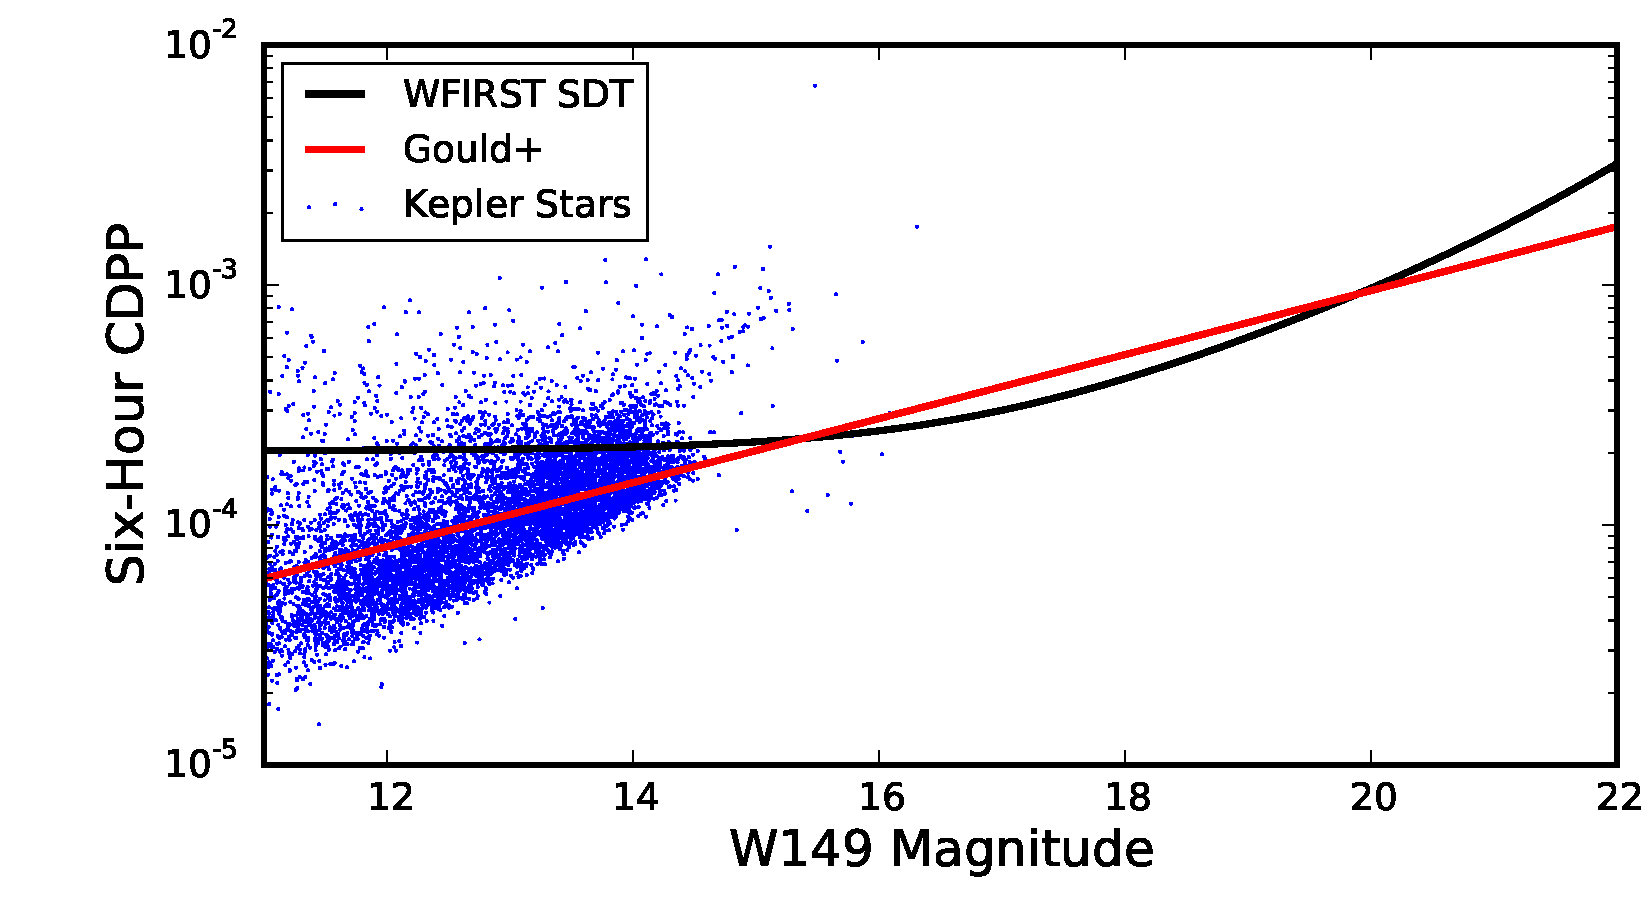
\includegraphics[width=0.75\textwidth]{chapter8/f1.pdf}}
\caption[Expected noise properties of \WF\ observing in the W149 bandpass as a function of
stellar magnitude]{Expected noise properties of \WF\ observing in the W149 bandpass as a function of
stellar magnitude. The black curve represents the estimates of the noise properties from the
\WF\ SDT report. The red curve represents the estimates of the noise properties from 
\citet{Gould15}, who focus on saturated stars to detect asteroseismic modes using \WF\ data.
In blue are actual observations of stars from \kep\ for comparison. In all cases, we report
the six-hour CDPP, or the noise averaged over six hours of observations.}
\label{fig:noise}
\end{figure}



\section{Detection of Transit Events}
\label{sec:transits}

To study the detectability of transiting planets with \WF, we
simulate transiting planet light curves with properties based on the
anticipated performance of \WF\, as described by \citet{Gould15}. We
assume a 52-second integration every 5 minutes and 6 evenly-spaced,
72-day campaigns over five years. We assume that all data will be
taken in the W149 band ($\textrm{0.927--2.000}\mu$m) with the exception of one data point
every 12 hours in the Z087 filter
($\textrm{0.760--0.977}\mu$m), i.e.\ one Z087 data point for every 47 obtained
in W149.

In this work, we assume the photometric noise is white, so that there are no correlations
between observations. 
Correlated noise can be the result of spacecraft systematics or stellar p-modes 
\citep{Gilliland10, Campante11}. 
The timescale for p-modes is inversely proportional with stellar density:
for G dwarfs, the granulation timescale is approximately five minutes; for M dwarfs, 
30 seconds. 
Like \kep\ data, for most stars observations will be 
spaced widely enough to capture a random phase of p-mode oscillations during each observation.
As \WF\ has significantly larger levels of photon noise, the correlated
stellar signals will be small by comparison, causing the while instrumental noise to dominate
over any red astrophysical effects.




\subsection{Hot Jupiters}
\label{sec:HJ}

The \WF\ microlensing mission intends to target more than one million stars
with $H < 14$ and 12 million stars with $H < 19$. To better understand the 
sensitivity of \WF\ to giant transiting planets, we simulate transits of a hot Jupiter
transiting a Sunlike star. 

We simulate individual transits of a hot Jupiter by injecting both realistic noise
and a planetary signal into simulated \WF\ data. We first create a star with
W149 $= 15.0$ to project a best-case scenario, where the noise expected to be at
the milimagnitude noise floor.
We then inject a Jupiter-sized planet on a 3.0 day orbit around this star,
which transits with impact parameter $b = 0.5$. 
The transit duration is approximately two hours.
Every fifteen minutes, starting at a random phase, we collect an observation
of the flux from this system: every twelve hours one observation is taken in 
Z087, while all other observations are in W149. 
We model the transit light curve with the transit model of \citet{Mandel02}. 
We calculate limb darkening coefficients in each bandpass using the online tool
developed and described in \citet{Eastman13}, which interpolates the 
\citet{Claret11} quadratic limb darkening tables. 

Unlike the \kep\ mission, each data point will consist of a single 
52-second observation, rather than a series of binned observations over 30 minutes.
Each observation will then sample one specific point on the transit light curve
as opposed to an integrated measure of the observed flux, meaning morphological
light curve distortions due to finite integration time will be virtually nonexistent in
\WF\ data \citep{Kipping10}.

The resultant ``observed'' transits are shown in Figure \ref{fig:HJtrans}.
These transits can be seen by eye, even in the case of single transit events.
Over the course of the mission, more than 150 transits of such a Hot Jupiter would be observed, leading
to approximately 1200 observations during the transit in the W149 bandpass.
Moreover, approximately two dozen observations during the transit will be collected
in the W089 bandpass, which might be useful for confirmation of the planetary 
nature of this signal (Section \ref{sec:confirm}).


\begin{figure}[htbp!]
\centerline{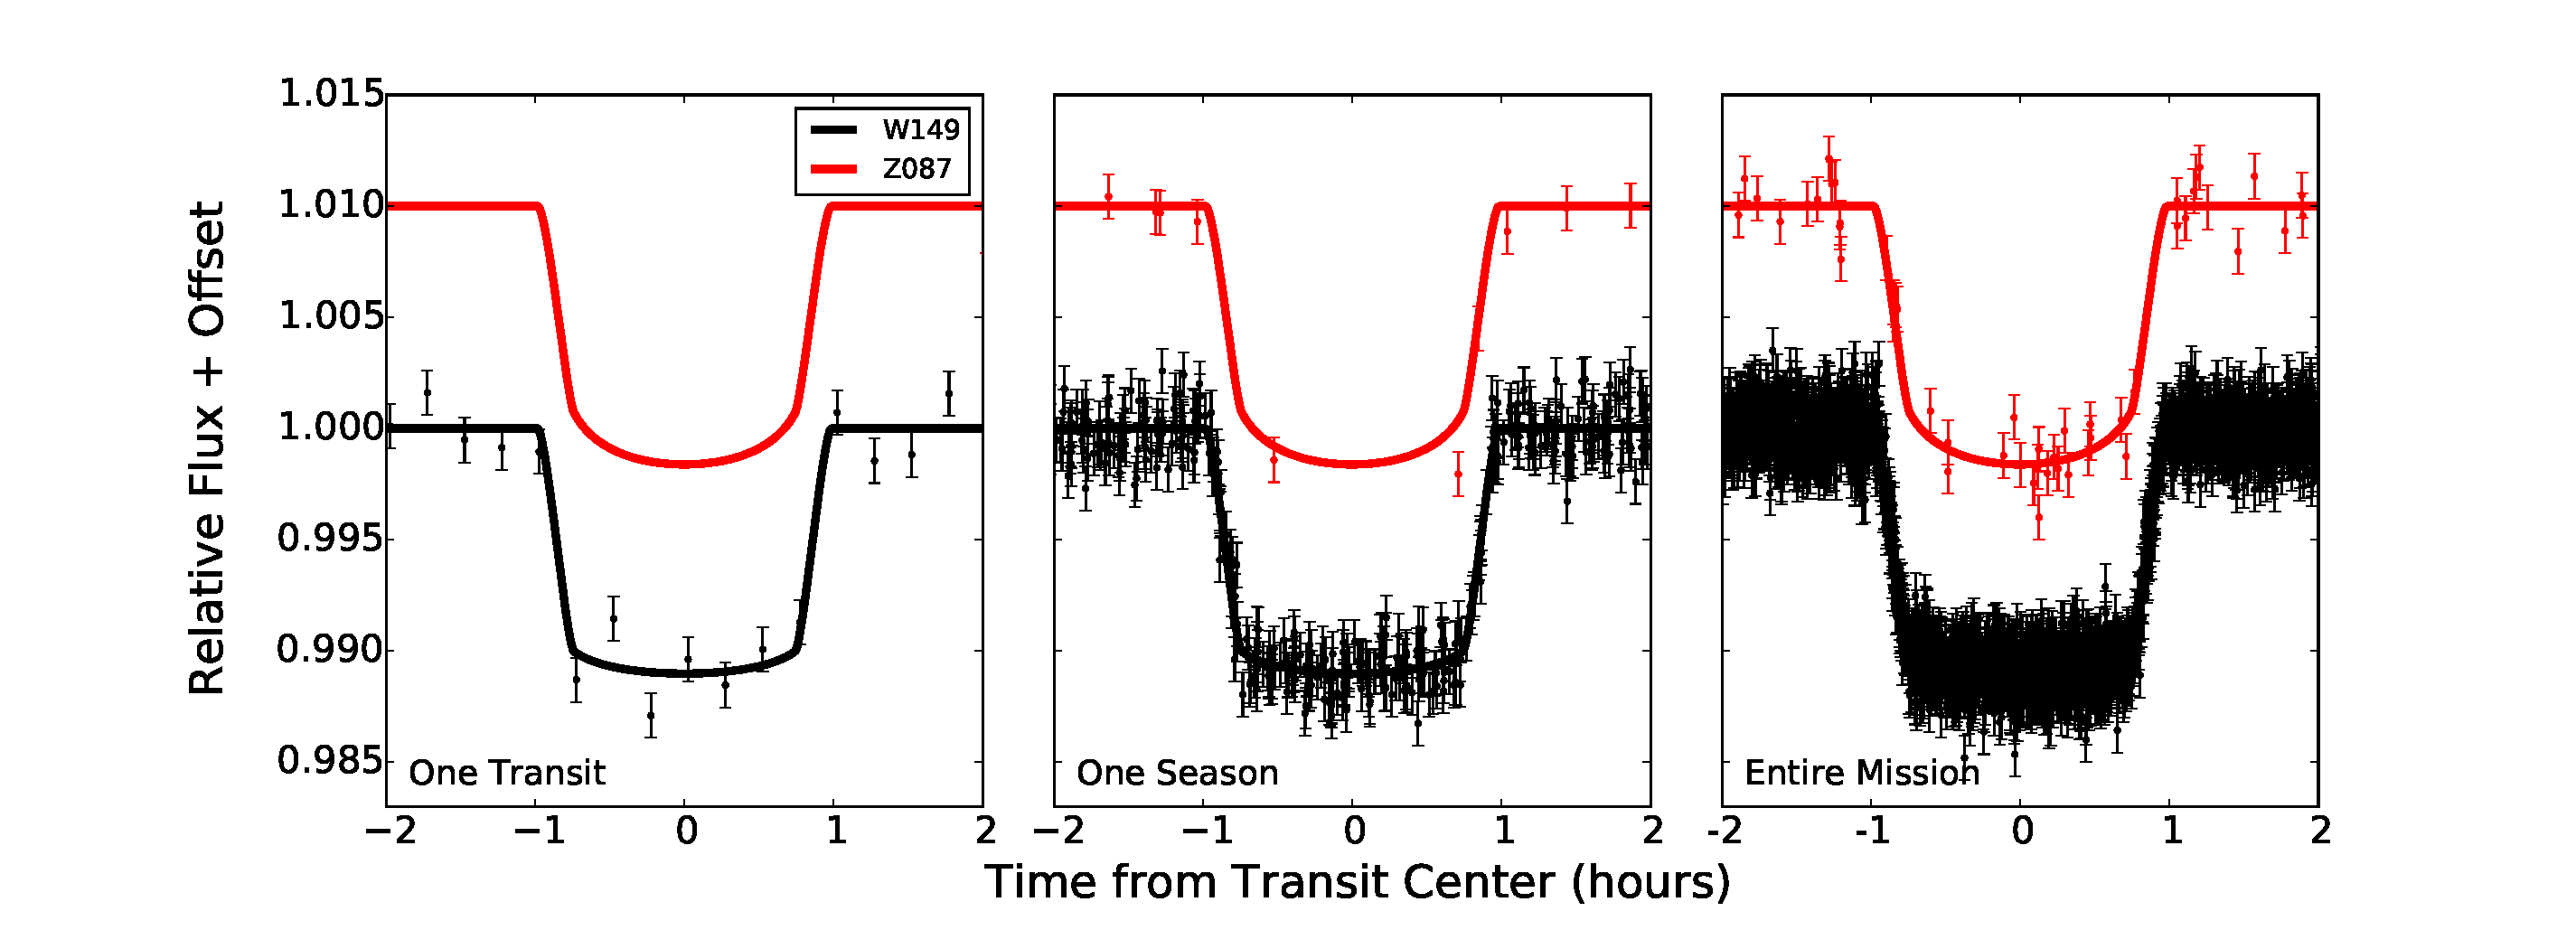
\includegraphics[width=0.9\textwidth]{chapter8/f2.pdf}}
\caption[Simulated transit photometry for a hot Jupiter in a three-day orbit
around a Sunlike star as observed with \WF.]{Simulated transit photometry for a hot Jupiter in a three-day orbit
around a Sunlike star with W149 $= 15$. In black is photometry from the
W149 bandpass; in red, the Z087 bandpass. The left panel corresponds to a single
transit. The middle panel corresponds to transits folded together over a 72-day
observing season, while the right panel corresponds to six such seasons over the
course of the mission.}
\label{fig:HJtrans}
\end{figure}

We then attempt to recover the transit signal in the data. By fitting transit
models and evaluating their likelihood, we measure a transit depth of
$0.998 \pm 0.002$ $R_J$, assuming perfect knowledge of the stellar host. 
This $\sim 500 \sigma$ detection of a transit implies
transiting hot Jupiters will be easily detected around $H \sim W149 = 15$ stars.

We can increase the level of the noise to determine the limiting magnitude
for which \WF\ will be effective at detecting hot Jupiters.
In the \kep\ mission, the threshold for a candidate planet transit was a $7.1\sigma$
detection of the transit, a standard we will apply here.
By inflating the size of our photometric uncertainties and repeating this exercise
we find that, assuming white noise, even when the single-point photometric precision
is 8\%, we are able to detect hot Jupiters in three-day orbits at $7.1 \sigma$ over
the course of the \WF\ mission.
The photometric limit is expected to be better than this value even
for stars with W149 $= 22.0$.
Typical extinction values in the $I$-band are 1-2 magnitudes \citep{Nataf13} and towards the 
galactic center $A_H/A_I = 3.2$, so we might expect less than one magnitude of
extinction in the W149 bandpass \citep{Nishiyama09, Nataf16}.
Even accounting for extinction, this limiting magnitude corresponds to Sunlike
stars well beyond $> 10$ kpc from the Earth, easily allowing us to detect hot Jupiter
systems around tens of millions of stars in total, at all galactocentric radii.

For the brightest stars, measuring a transit signal to a precision of 
$0.2\%$ implies photometric precision of approximately 20 parts per million
when binned over two-hour intervals and phase-folded on a two-day period.
This is significantly below the precision needed to detect relativistic Doppler
beaming in the light curve \citep{Loeb03, Faigler11}, but could be used to detect
false positive events such as transiting brown dwarfs and low-mass stars masquerading
as hot Jupiters (see Section \ref{sec:PC}).


\subsection{Sensitivity to Small Planets}
\label{sec:small}

Given the high signal to noise expected for hot Jupiters transiting the brightest stars
observed with \WF, we might expect the telescope to be sensitive to planets transiting
stars significantly smaller than Jupiter as well.
We can determine how small a planet would be detectable by \WF\ as a function of planet
orbital period and radius. 
We will repeat this exercise for stars at W149 $= 15$ and $\textrm{W149} = 19.5$; there are 
expected to be 1 million and 12 million stars brighter than these limiting magnitudes,
respectively.

To calculate our sensitivity to planets in general, we first create a planet with a radius and an orbital
period drawn from log-flat distributions over the ranges $[1, 16]R_{\oplus}$ and $[1,72]$ days, respectively. We then assign an impact parameter for each
transiting planet drawn from
a uniform distribution over the range $[0, 1]$. 
We assume a circular orbit for the planet and calculate the relative position of the 
planet and star, applying the transit model of \citet{Mandel02}.
We draw an observation every fifteen minutes.
We assume white noise with the photometric
precision given by the \citet{Gould15} curve of Figure \ref{fig:noise}, removing one observation every twelve hours
when \WF\ is collecting $z$-band data instead.
After all transits have been simulated, we phase-fold on the known period and measure
the significance of the observed transit depth. 
If it is larger than $7.1\sigma$, we declare this transit detected; otherwise, we declare
it missed.
We also require at least two transits during at least one season to be detected.
By repeating this procedure many times with many different planet sizes and periods,
we can map the sensitivity of \WF\ to small planets. The results are shown in Figure
\ref{fig:Sensitivity}.

\begin{figure}[htbp!]
\centerline{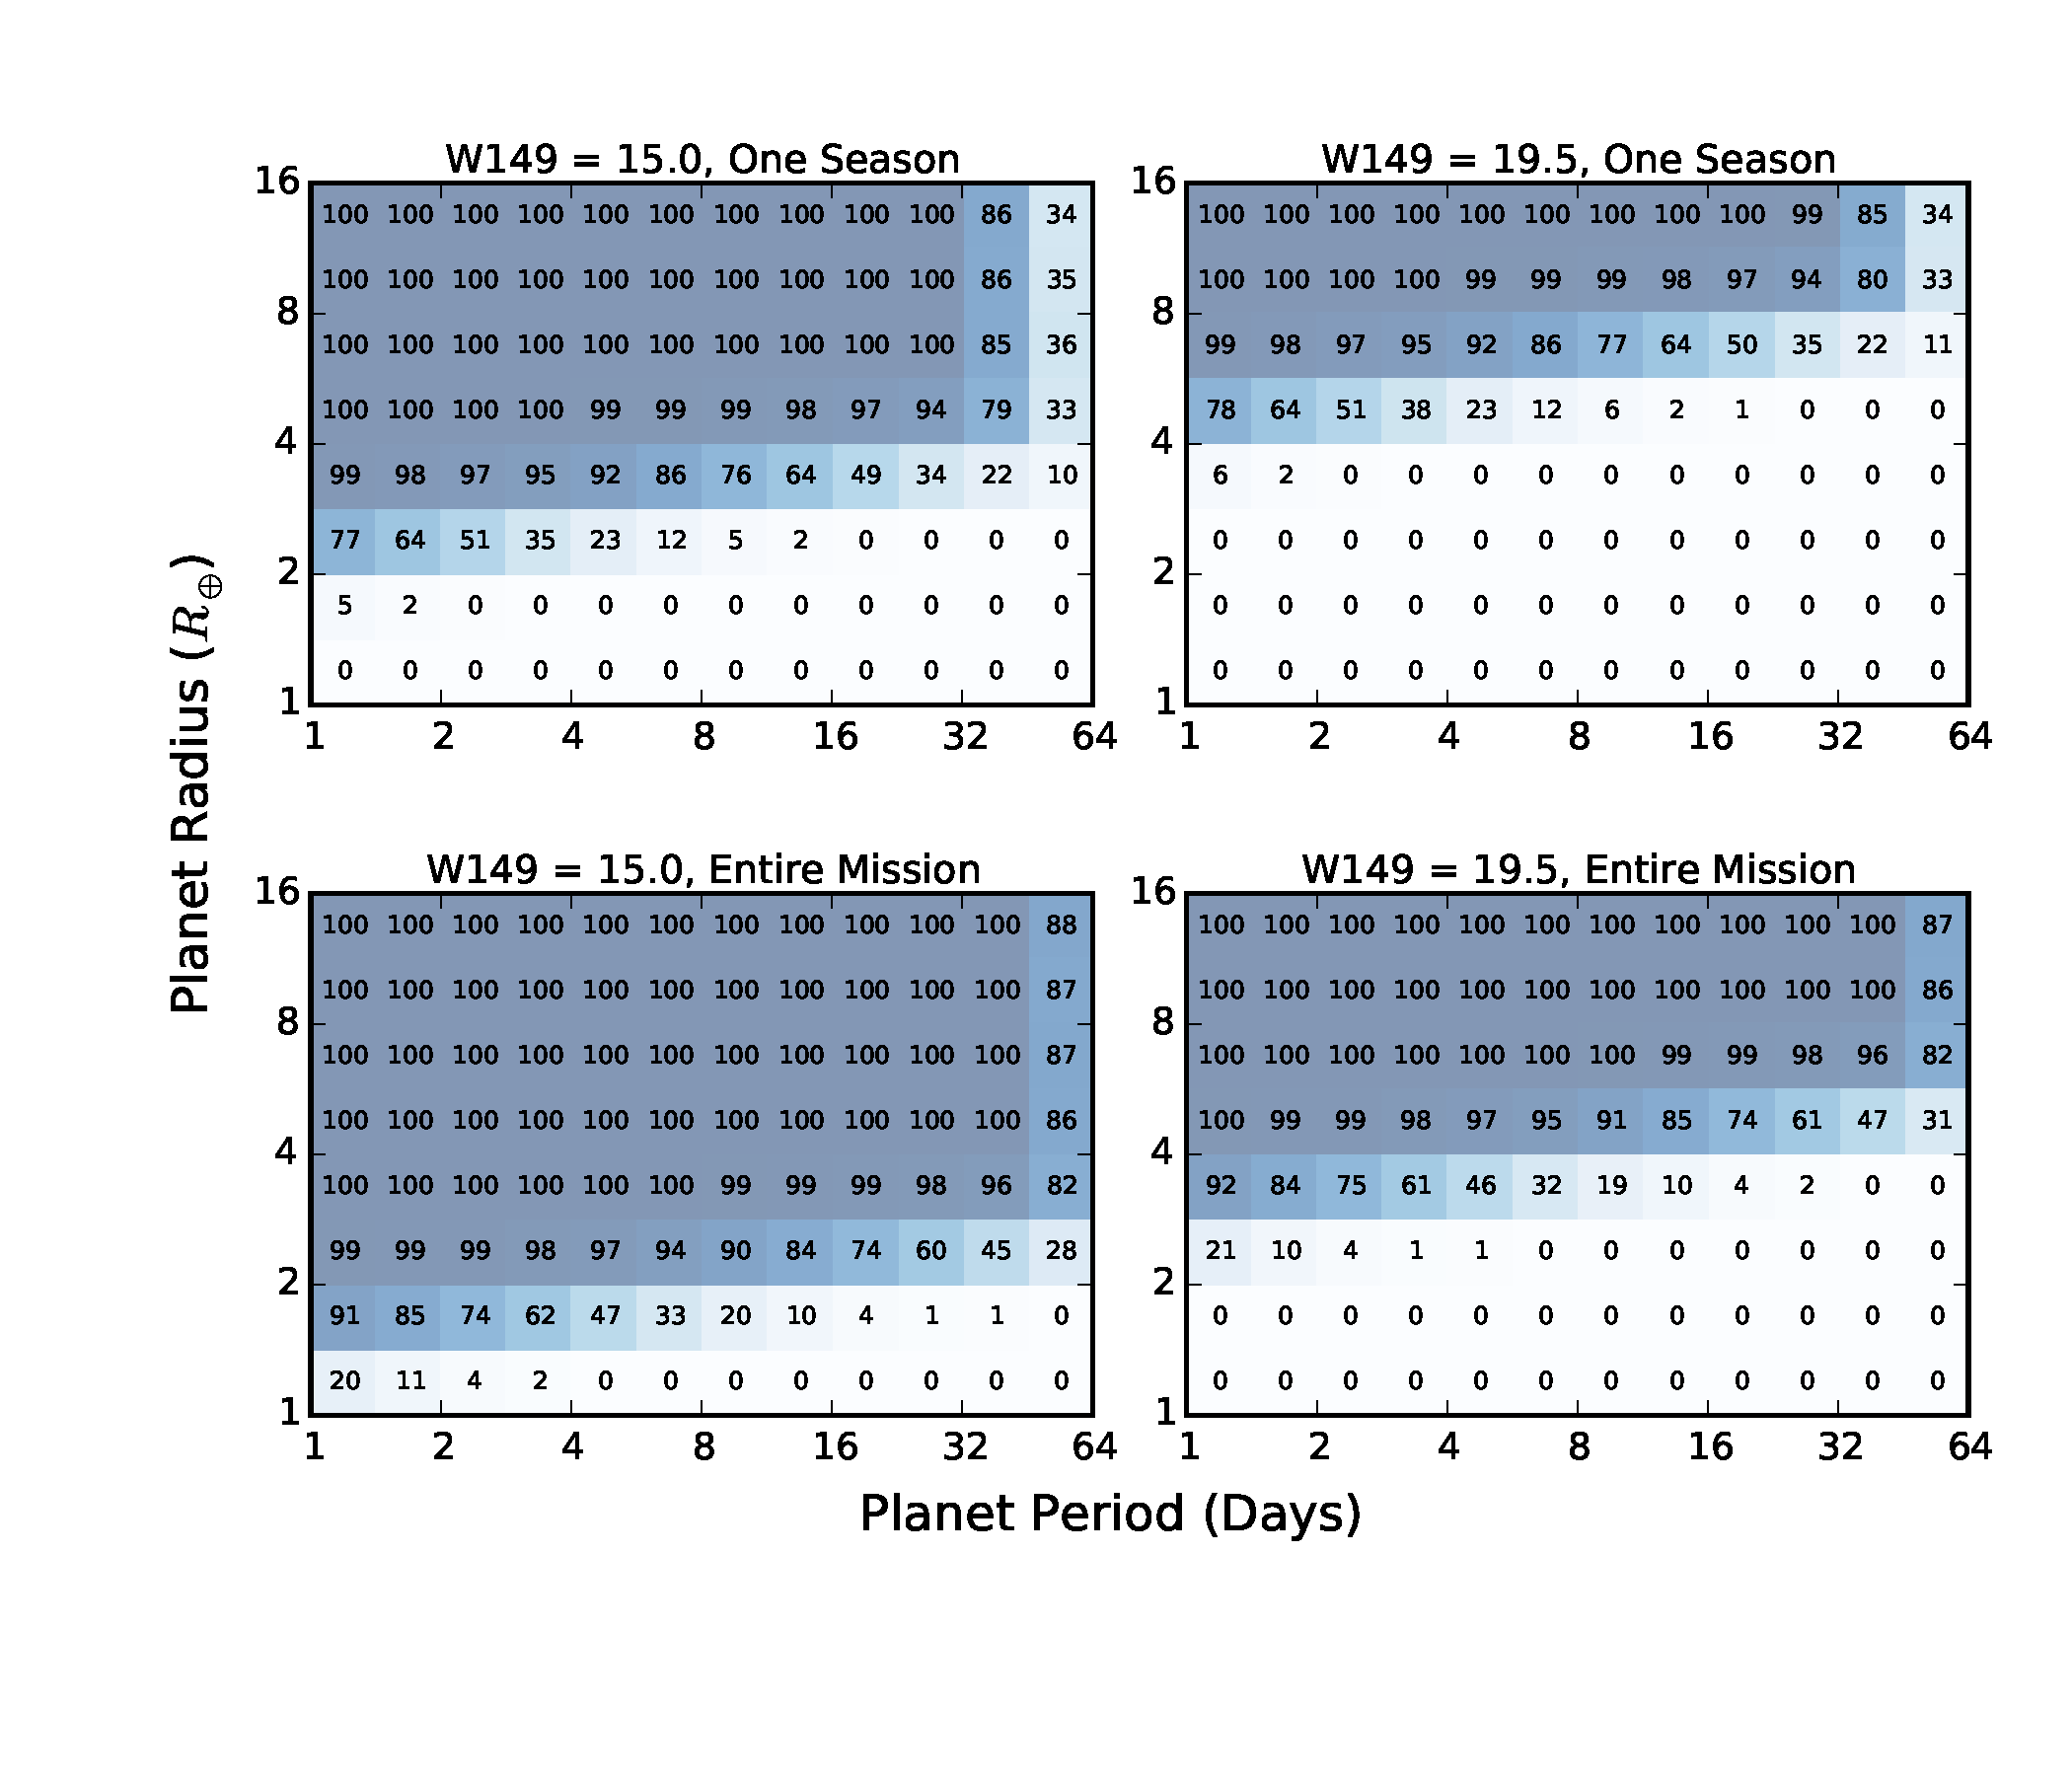
\includegraphics[width=0.98\textwidth]{chapter8/f4.pdf}}
\caption[Fraction of planets of given sizes and orbital periods expected to be detected by \WF.]{Detectability of planets transiting a Sunlike star in simulated \WF\ data by analyzing (top) one season of data and (bottom) data from the entire mission.
Around very bright stars (W149 = 15.0) nearly all Neptune-sized planets and larger with
orbital periods shorter than the seasonal baseline will
be detected in a single season of data.
To qualify as a detection, we require at least two transits in a single observing season,
but not necessarily in all seasons.
}
\label{fig:Sensitivity}
\end{figure}

We find that, for the brightest stars observed by \WF, Neptune-sized planets with
orbital periods shorter than one month will be easily detected in a single season of data. 
The mission will also recover many mini-Neptunes with periods shorter than 20 days, and
is likely to recover a small number of planets smaller than 2 \rearth\ with 
periods shorter than two days. 
Over the entire mission, \WF\ will be sensitive to a few Earth-sized planets 
with orbital periods shorter than two days orbiting the brightest stars.
Of the 12 million stars with $\textrm{W149} < 19.5$, the prospects for detecting super-Earths
or mini-Neptunes are much lower, but the mission will detect the majority of  
Neptune-sized planets with periods less than a month and all transiting Jupiter-sized
planets in that period range as well.

There is a strong decay in the sensitivity of \WF\ to transiting planets as a function
of planet radius compared to planet period. This is not surprising, and the same effect
is seen in \kep\ data \citep{Burke14, Mullally15, Rowe15}. 
The transit duration is proportional to $P^{1/3}$ and the observed depth
depends on the projected surface area of the planet, so
the phase-folded transit signal depends on $R_p^2 P^{-2/3}$ \citep{Seager03}. Therefore a change in the orbital period should have a weaker effect than a change in the size of the planet, as we
observe here \citep[see also][]{Carter08}.

\subsection{Single Transit Events}

\WF\ will, in addition to detecting thousands of planets with short orbital periods, be
sensitive to singly transiting events of giant planets in more distant periods.
The best measurements of the occurrence rates of these planets is understood from 
combining observations of long-term RV accelerations with direct imaging surveys 
\citep[Gonzales et al. in prep]{Montet14}. 
There are only a few dozen such planets detected in the \kep\ data, detected largely
through visual inspection \citep{Wang15b, Uehara16}. 
For a given planet in a long orbital period, the probability of transit is directly
proportional to the observing baseline.
The \WF\ observing baseline is a factor of four shorter than that of \kep, but as the
total number of stars observed by \WF\ is nearly two orders of magnitude larger than 
\kep, we expect visual inspection of \WF\ data to uncover on the order of one thousand
additional giant planets. 
As even single transit events can provide unique information about transiting planets
\citep{Yee08, Osborn16}, these data will 
improve our understanding of planets at wide separations.


\subsection{Deriving Transit Times from \WF\ data}
\label{sec:ttvs}



The sensitivity to short-period planets smaller than Neptune in a single season of 
\WF\ data implies that we may be able to detect variations in the time of transit
across the mission.
These transit timing variations (TTVs) have been used previously to confirm the 
planetary nature of transiting signals \citep{Holman10, Fabrycky12, Ford12TTV, Xie13}, 
to detect the presence of non-transiting
planets \citep{Ballard11, Nesvorny12, Nesvorny13}, and to infer masses and
eccentricities of planetary systems 
\citep{Hadden14, Jontof-Hutter15, Jontof-Hutter16}.
While TTVs have been observed in \KT\ data \citep{Barros15}, the short time baseline makes
these detections the exception rather than the rule.
Given that \WF\ will observe the same fields over five years, we might expect to detect 
deviations from a linear transit ephemeris if our sensitivity to transit times is small enough.

To this end, we simulate transit events in order to estimate the precision to which we will
be able to measure transit times. We model our benchmark system after Kepler-9b and Kepler-9c, the first planets confirmed via TTVs \citep{Holman10}.
We use orbital periods for the two planets of 19.2 and 38.9 days. 
Given that less massive planets more often exhibit TTVs than more massive planets 
\citep{Mazeh13}, we simulate planets near the bottom of our detectability
contours in order to understand the limits for detecting TTVs with \WF. Hence, we assume the two planets are mini-Neptunes with masses of $10$ \mearth\ and radii of $3$ \rearth. These are significantly smaller than the real Kepler-9 planets leading to smaller TTVs and larger uncertainty in the measured time of transit center.
We simulate transits of these planets orbiting a Sunlike star with W149 = 15.0, so that
the photometric precision on each data point is 1 part per thousand, assigning 
impact parameters at random. 

We focus on TTVs of the inner planet, because more transits will be observed over the course of the \WF\ mission.
We fit a transit model to the simulated data for the inner planet, fixing the limb darkening to that
expected for a Sunlike star in the H-band but allowing all other parameters to vary. The measured transit times are shown in Figure \ref{fig:ttv}.
Simulating many transits, we find a median uncertainty in the measured transit time
for each individual transit
of 28 minutes. 
We then phase-fold all observed transits inside an observing season, finding a median
uncertainty on the average time of the folded transit of 15 minutes (Figure \ref{fig:ttv}). 
Given the large number of observed TTV signals in \kep\ significantly larger than this
timing precision, we expect \WF\ to be able to efficiently measure TTVs.




\begin{figure}[htbp!]
\centerline{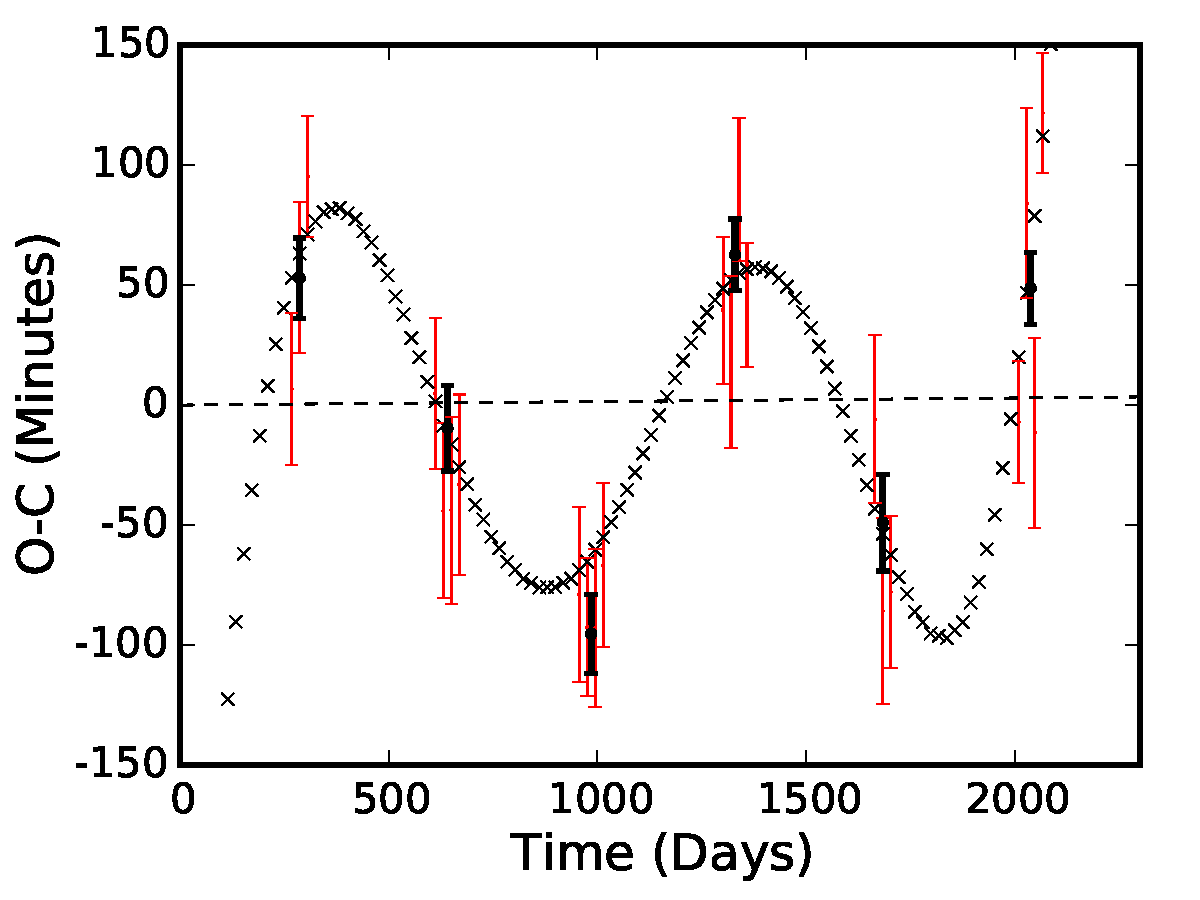
\includegraphics[width=0.75\textwidth]{chapter8/f3a.pdf}}
\caption[Simulated TTV signal from an interacting two-planet system as observed by \WF.]{Simulated TTV signal from a two-planet system as observed by \WF\ (see Section \ref{sec:ttvs}). 
Gray X labels correspond to the actual deviation form a linear ephemeris for each 
individual transit. For those observed during a simulated \WF\ season, typical
uncertainties are added to the observed time of transit with data shown in red. The black
points correspond to binned observations over an entire season. This hypothetical system
would be confirmed by TTV observations in \WF\ data.}
\label{fig:ttv}
\end{figure}



Accurate determinations of transit times is more difficult in the presence of 
starspots, which induce a correlated signal in the light curve.
As a planet transits the stellar disk, if it passes across a 
relatively dark spot this will cause a distortion in the shape of the light curve.
Moreover, spots at other stellar latitudes can cause the out-of-transit flux baseline
to vary, complicating the measurement of the time of transit.
\WF\ will observe in the near-IR, where the effects of starspots are significantly 
minimized due to their lower contrast, reducing the possibility of significant 
starspot-induced timing errors.

\section{Galactic Exoplanet Demographics}
\label{ss:yield}


We can simulate realistic populations of both stars in the bulge and their exoplanets 
to estimate how many transiting planets \WF\ will be able to detect over the course of its mission.
To simulate a realistic estimate of the stellar population in the bulge, we develop a 
galactic population generated from the online Besan\c{c}on models of the galaxy \citep{Robin03}.
To convert the returned apparent magnitudes to near-infrared simulated photometry, we
apply the transformations of \citet{Bilir08}. 
We then apply a correction for interstellar extinction assuming the \citet{Cardelli89}
extinction law with $R_v = 2.5$, following \citet{Nataf13}.
From the derived JHK magnitudes, we approximate the W149 magnitude for each star
by assuming W149 = (J+H+K)/3.

We then apply a series of corrections to turn the Beasan\c{c}on models into a realistic
simulation of the stars observed by \WF. The Beasan\c{c}on model outputs the properties and numbers of stars along a given sightline within a certain solid angle.
Because each simulated field is not a perfect match to the \WF\ field, we weight each simulated star by the fraction of the simulated field that falls in the \WF\ field.
We then apply a correction for the mass function in the bulge. 
The model assumes stars in the bulge follow the Salpeter IMF \citep{Salpeter55}.
We downweight stars of mass $M< 0.5$ \msun\ by a factor of $0.5/M$, which approximates
the IMF of \citet{Kroupa01}.
We then apply a uniform correction to all stars to match the overall number of 
bulge main sequence stars near the \WF\ fields as measured by \citet{Calamida15}.

We then inject planets around the main-sequence
dwarf stars brighter than W149 = 19.5 in our simulation. Since the 
\WF\ sensitivity in the radius-period plane (Figure \ref{fig:Sensitivity}) is limited to a region of parameter space 
well-sampled by the \kep\ mission in the original \kep\ field.
We assign planets around solar-type FGK stars following the planet occurrence estimates 
of \citet{Howard12}.
We assign planet radii and orbital periods following the ``Cutoff Power-Law Model'' of Table 5 of
that paper, and bulk occurrence rates for each spectral type following the authors' Table 4.
For M dwarfs, we follow the relations of \citet{Morton14}, specifically their ``logflat+exponential''
model of the period distribution from their Figure 7 and the radius distribution from their Figure 6.
This leads to considerably smaller numbers of giant planets injected around M dwarfs than more massive
stars, in line with observations from \kep.

We simulate the transits of these planets following the same prescriptions as in Section \ref{sec:transits}.
We assume the noise properties of \citet{Gould15} and we estimate limb darkening parameters by interpolating our stellar parameters onto the
quadratic limb darkening grids of \citep{Claret11}, taking $H-$band as a proxy for W149. We limit the range of orbital periods to $P<72$ days.
We declare a planet detected if we 
recover its transit signal at $7.1\sigma$ and observe at least two transits in any one season.

The results are shown in Figure \ref{fig:yield1}. We expect \WF\ to detect approximately 13,000
transiting planets orbiting bright dwarf stars, the majority being giant planets orbiting F and G stars.
The mission will also detect more than 100 planets smaller than Neptune, the majority of which will
be orbiting M dwarfs. We note that our prescription for the photometric precision does not significantly affect the bulk numbers of planets detected.

The number of transiting planets from this simulation assumes that the occurrence rate is the same in the \WF\ field as in \kep.
However, radial velocity surveys have unveiled a correlation between giant planet occurrence and stellar 
metallicity \citep{Fischer05, Johnson10a}, while the presence of small transiting planets appear 
to not be affected by the host star's metallicity \citep{Buchhave15}. Given that the median metallicity of dwarfs in the \WF\ field is [Fe/H] = 0.25, and most of the planets detected by \WF\ will be giants, this correlation could significantly
influence the number of giant planets detected. 

We account for this metallicity effect by injecting planets according to the radius and period distribution of the
\kep\ field, but increasing the likelihood of a star hosting a planet according to the star's 
metallicity in our sample.
Following \citet{Johnson10a}, who find planet occurrence scales as $10^{1.2\textrm{[Fe/H]}}$, we 
modify the likelihood of all planets with radii larger than 5 \rearth\ by this factor.
For the median star ([Fe/H] = 0.25), this factor increases giant planet occurrence by a factor of two.
We then repeat our simulations with our modified planet occurrence, with the results shown in Figure \ref{fig:yield2}. 
In this case, we detect more than 30,000 transiting planets over the six seasons of the \WF\ mission.
As expected, the number of small planets is unchanged, with the gains made entirely in the
population of planets larger than Neptune. 
\WF, by completing this survey, will provide the best assessment of the effects of high 
metallicity on the population of giant planets, providing clues to the formation and evolution
of these systems.

Finally, we note that our analysis is limited to dwarf stars towards the bulge brighter
than W149 = 19.5. While planets have been detected
around evolved stars \citep{Lillo-Box14, Barclay15, Quinn15}, their occurrence rates
are too poorly understood to enable a reliable estimate of their yield in \WF. 
However, given the photometric precision (Section \ref{sec:kepler}) and scaling from Section \ref{sec:transits}, giant planets will be detectable around evolved stars (i.e. given that $3R_{\oplus}$ planets are detectable around a $1 R_{\odot}$ star, a $12R_{\oplus}$ planet should be detectable around a $4 R_{\odot}$ star.).
As \WF\ will observe large numbers of evolved stars towards the bulge, it will provide
the best measurement to date of the occurrence rate of giant planets in short orbits
around evolved stars.




\begin{figure}[htbp!]
\centerline{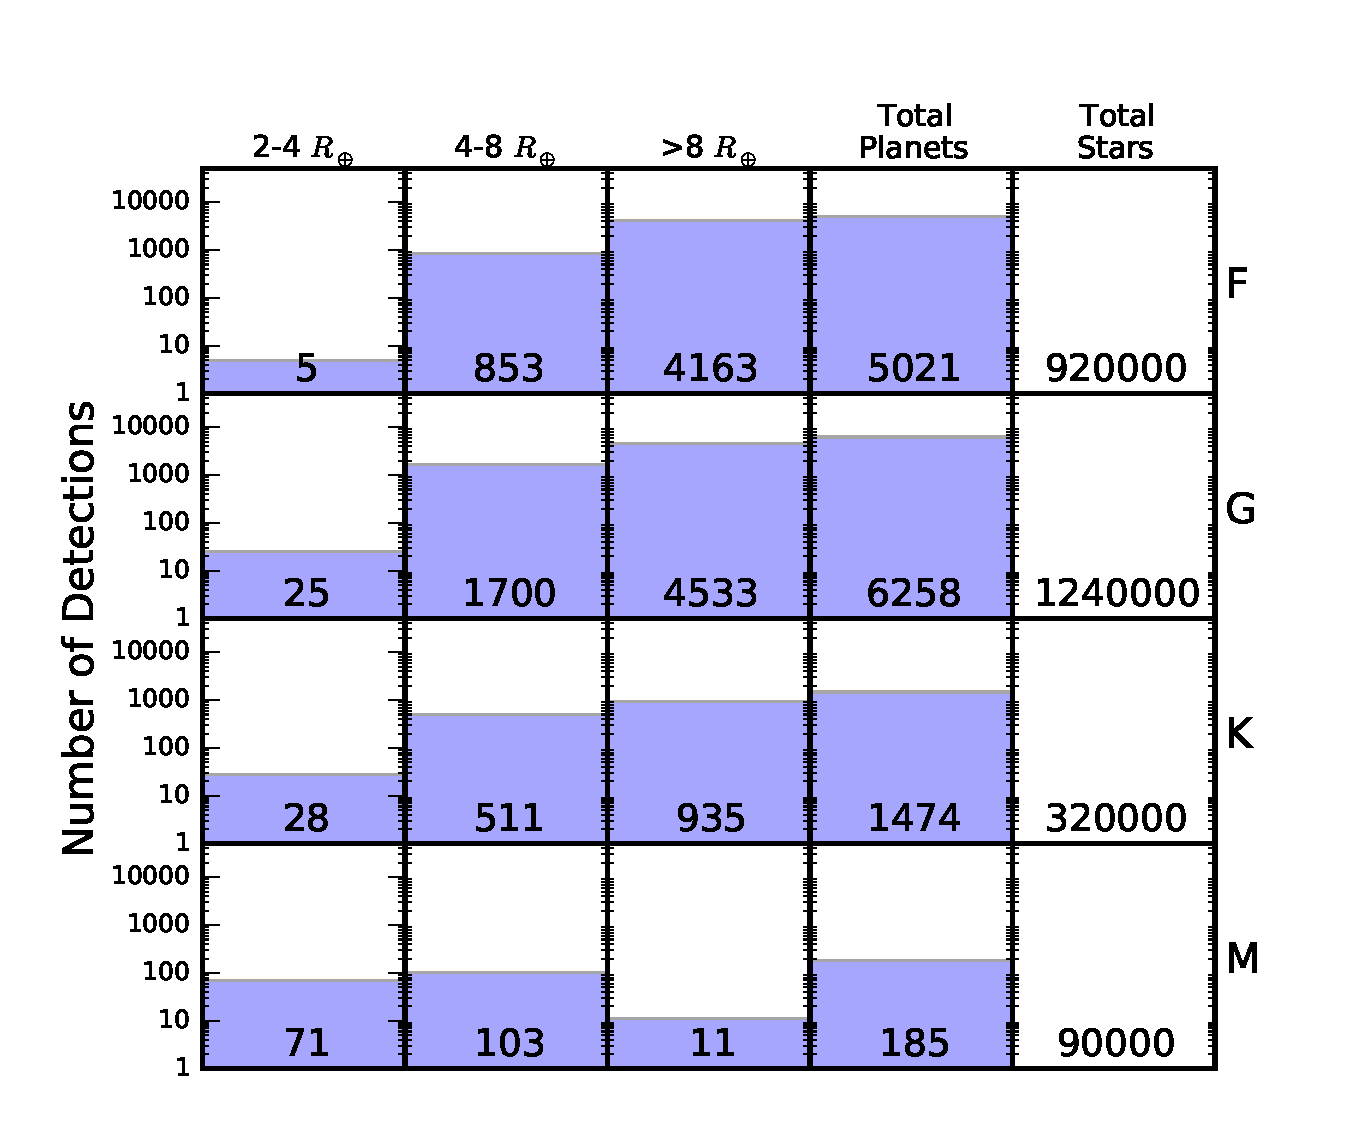
\includegraphics[width=0.75\textwidth]{chapter8/f5b_n.pdf}}
\caption[Expected transiting planet yield from \WF\ assuming planet occurrence is the same as that in
the \kep\ field]{Expected yield of transiting planets orbiting dwarf stars
  brighter than W149 = 19.5 in the \WF\ data as a function of
  planet size and stellar type, assuming the planet occurrence is the same as that in the \kep\ 
  field. \WF\ will detect thousands of Jupiter sized planets, but also more than 100 planets
  smaller than Neptune, mainly around M dwarfs. }
\label{fig:yield1}
\end{figure}


\begin{figure}[htbp!]
\centerline{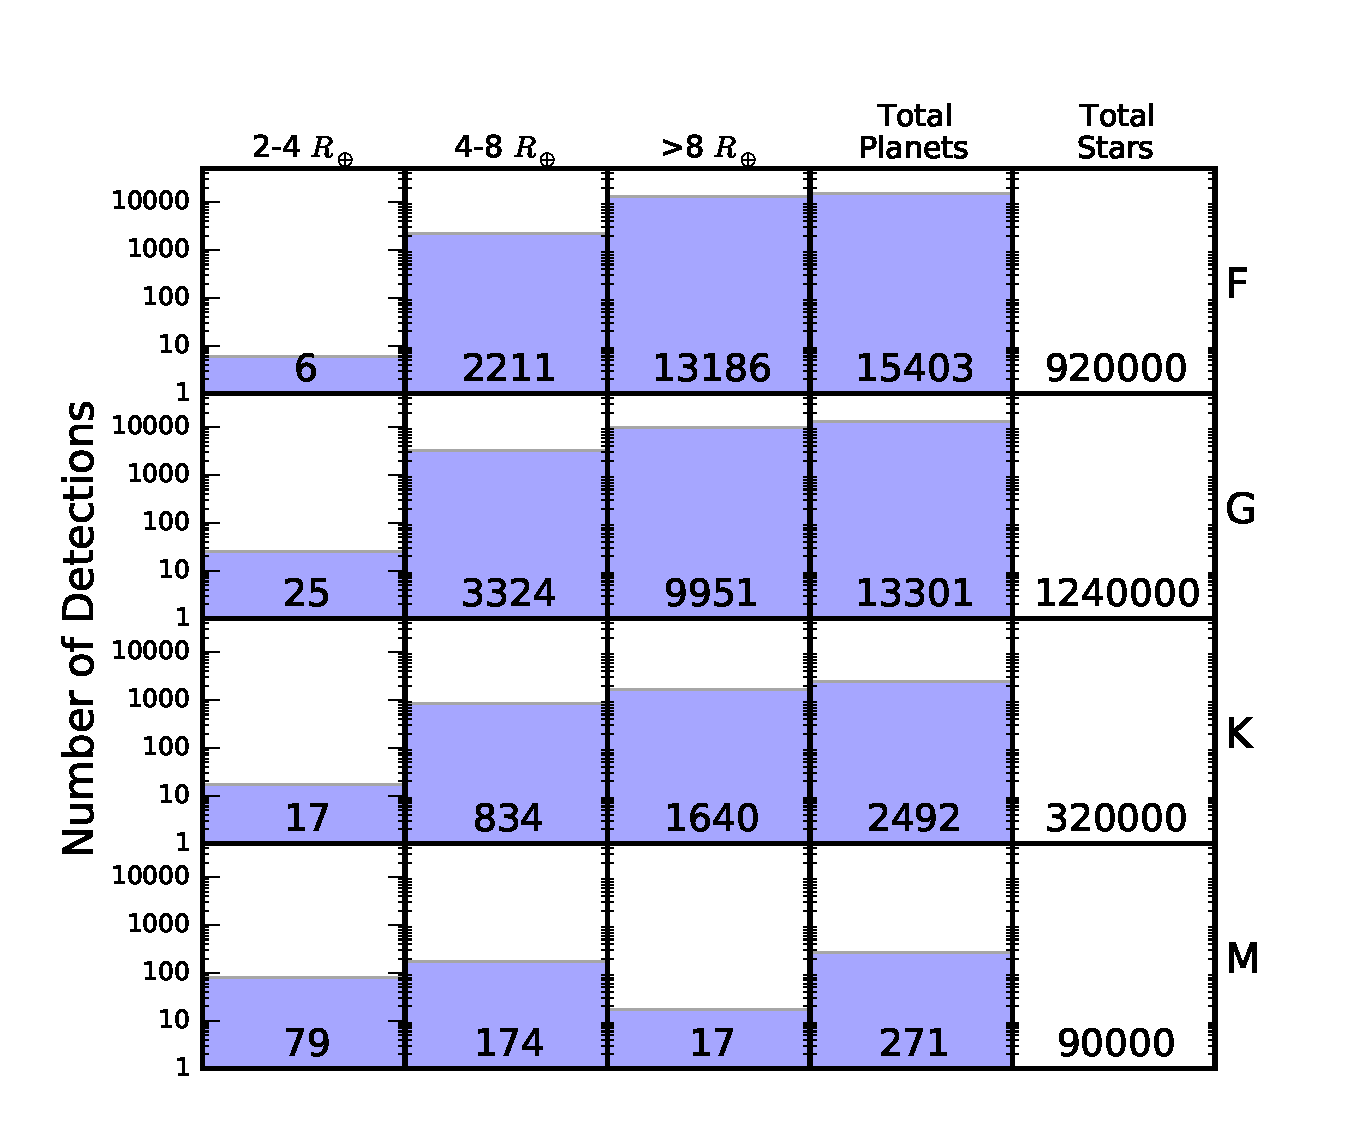
\includegraphics[width=0.75\textwidth]{chapter8/f5a_n.pdf}}
\caption[Expected transiting planet yield from \WF\ assuming giant planet occurrence follows the same
relation with metallicity as observed in the solar neighborhood]{The same as Figure \ref{fig:yield1}, assuming planet occurrence for planets
larger than 5 \rearth\ follows
the relation with stellar metallicity as observed in the solar neighborhood,
following \citet{JohnsonApps09}. Under these assumptions \WF\ will detect 
more than 30,000 planets.}
\label{fig:yield2}
\end{figure}



\section{Confirmation of Transiting Planetary Systems}
\label{sec:confirm}


The major challenge for transiting planet studies is to verify that the observed transiting object is a planet rather than a false positive. 
Multiple astrophysical events can be mistakenly identified as transiting planets. 
First, because of degeneracy pressure, Jupiters, brown dwarfs, and low-mass M stars all have similar radii \citep{Chabrier97}.
Hence, detection of a Jupiter-radius transit depth alone is insufficient to claim a planetary detection. 
Second, a false positive can occur in the case of blended light, when the star in 
question in the aperture is actually the combined light of multiple stars.
For example, a background unknown eclipsing binary could be blended with the primary target
star.
Similarly, the primary itself could be an eclipsing binary blended with the chance alignment
of a background star or the light of a hierarchical triple third star.
These degeneracies are easily resolved with RV observations, but those will not be possible for most \WF\ transit candidates.
However, previous studies have shown in the case of \kep\ that it is possible to validate transiting planet candidates by ruling out various false positive scenarios \citep{Morton12, Morton16}. Here and in Section \ref{sec:validate}, we explore various means to confirm, validate, or rule out false positives for \WF\ transiting planet candidates.




\subsection{TTVs}

The most straightforward way for \WF\ to confirm the planetary nature of transit signals from small
planets is through the detection of transit timing variations.
In Section \ref{sec:ttvs}, we showed that TTVs are easily recovered for a scaled-down version of the Kepler-9 system.
The exact nature of any TTV curve depends on the architecture of any particular TTV 
system: two planetary systems with identical planets but different orbital eccentricities,
arguments of periapsis, or longitudes of ascending node would exhibit different TTV
signals. 

A full simulation of this stuff is beyond the scope of this paper. However, we note that
the TTV catalog of \citet{Holczer16} lists 571 \kep\ planet candidates with
TTV signals larger than 30 minutes and 176 with TTV signals larger than 60 minutes.
Many of these planets will be too small to be detectable in the relatively noisier
\WF\ data.
Considering these numbers,
based on the number of planets we expect \WF\ to be able to detect and the timing precision 
we expect the mission to achieve on individual transits \ref{sec:ttvs}, 
we expect more than 100 TTV detections over the observing campaign. 

\WF\ will have the added benefit of an observing baseline larger than five years, longer
than the original \kep\ mission. TTVs that manifest themselves on longer timescales, 
such as those caused by non-resonant planets, Roemer delay
from a hierarchical binary star, or orbital evolution of a giant planet in a short orbit \citep{Ragozzine09, Maciejewski16},
will be more likely to be detectable with \WF.

While TTVs will be extremely useful to confirm the planetary nature of small planets,
given the observing strategy of \WF\, it is unlikely that TTVs will be able to robustly
determine masses.
To verify this claim 
we use TTVFast \citep{Deck14} to integrate a dynamically interacting planetary system 
compare the result to the simulated transits from Section \ref{sec:ttvs}
during six hypothetical \WF\ observing seasons. 
We purposefully schedule the \WF\ seasons to coincide with the smallest observed TTV
signal to simulate a worst-case scenario.
For each observed transit, we add a random offset drawn from a uniform distribution on the
range [25 minutes, 40 minutes], similar to the predicted scatter on measurements of the times 
of individual transits, and assign an uncertainty on the observed time of transit
equal to this value. 

Fitting only the transits of the inner planet, we find that a dynamically interacting
planet model fit the data considerably better than a linear ephemeris ($\Delta \chi^2 = 72$). 
In this case, these planets would be easily confirmed via \WF\ observations:
only very contrived examples of planets with these masses, orbital periods, and 
eccentricities produce nondetectable TTVs. 
However, the inferred masses of the transiting planets are a function of the unknown
eccentricity: a pair of 10 \mearth\ planets or a pair of 25 \mearth\ planets can both
explain the observed TTVs.

In many cases, while confirmation of the planetary nature of systems will be easy, 
the large gaps between seasons will
complicate determination of unique solutions of the masses of individual planets
and induce
degeneracies between their masses and eccentricities.
For the brightest stars, it may be possible to identify particular transits that would
be useful for precise determination of planet masses and to follow up these planets with
ground-based
facilities at these specific times.


\subsection{Secondary Eclipses}


It is unlikely that TTVs will be useful for confirmation of more than a few of the 
hot Jupiters detected by \WF.
TTVs depend on the existence of a second planet, but
giant planets are most often detected in isolation, without a transiting companion
\citep{Steffen12c}.
There is only one hot Jupiter system with detected TTVs induced
by the presence of an additional planet \citep{Becker15}. 
However, it is possible that these planets will be confirmed by observations of their
secondary eclipses. The depth of the secondary eclipse yields a measurement of the
brightness temperature, and thus the flux in that bandpass \citep[e.g.][]{Charbonneau05}.

From \kep\ data alone it is difficult to confirm planets via secondary eclipses.
While \kep\ found thousands of planets, it was only able to confirm planetary systems
via detection of their phase curves and 
secondary eclipses for a handful of these \citep[e.g.][]{Esteves13, Quintana13, Angerhausen15}. 
Because the \kep\ bandpass spans approximately $0.4-0.9$ $\mu$m, near the peak of a typical
stellar spectrum but far bluer than the typical planetary spectrum, only the hottest,
largest planets are detectable by their own emission. 
However, \WF, with its primary bandpass spanning 0.927-2.000 $\mu$m, will be significantly 
more effective at observing planetary emission directly. 

To determine the feasibility of observing secondary eclipses with \WF, we consider the case of a hot Jupiter transiting a Sunlike star, similar to the
case of Section \ref{sec:HJ}. 
We can determine the relative flux of the two objects across the \WF\ bandpass to determine
the integrated secondary eclipse depth expected.
We assume a Jupiter-sized planet with an equilibrium temperature of 1200 K orbiting a 
Sunlike star.
We obtained a theoretical spectrum for a 1200 K and 5800 K object from the BT-Settl
spectral library of \citet{Baraffe15}, using the updated CIFIST2011\_2015 models.

We then integrate these spectra across the W149 filter, assuming a planet the size of 
Jupiter being eclipsed by a star the size of the Sun.
We predict, for this system, a secondary eclipse depth of 350 parts per million, approximately equal to the transit depth of a $2$ \rearth\ planet.
From Figure \ref{fig:Sensitivity}, we expect detections of secondary eclipses to be
rare around stars with $\textrm{W149} = 19.5$, but common around the million stars with 
W149 brighter than 15.0.
For the bright stars, we expect to detect approximately one-third
of planets of this size and orbital period in one season of \WF\ data, and nearly
all planets across the entire mission, so the same will be true for detecting secondary
eclipses. 

We are likely to recover secondary eclipses of the hottest planets even more effectively.
The planetary equilibrium temperature scales as $a^{-1/2}$, and hot planets are often 
inflated relative to their cooler cousins \citep{Charbonneau00, Showman02}, both increasing
the depth of the secondary eclipse:
WASP-12b's secondary eclipse depth across this bandpass is nearly 2 parts per thousand
\citep{Croll11, Stevenson14b}, corresponding to the same depth of a transit of a 
4.9 \rearth\ planet.
We can then expect observations of secondary eclipses to be useful for confirmation of
hot Jupiter systems.


Secondary eclipses will provide additional benefits to our understanding of the population
of transiting hot Jupiters beyond simply confirmation.
The timing of the secondary eclipse depends on the eccentricity vector $e \cos \omega$,
enabling statistical analyses of hot Jupiter eccentricities and detections of non-circular
planets, providing clues into the dynamics of hot Jupiter formation.


\section{Validation of Transiting Planetary Systems}
\label{sec:validate}


\subsection{Z087 Photometry}

Transits of a dark object across the face of a star should be, to first order, achromatic.
False positive events caused by eclipsing binaries, where multiple objects are
self-luminous, will have wavelength-dependent depth variations as different portions
of the stellar SEDs are sampled at different bandpasses.
Multiband photometry can then be used to separate transiting planets from 
background eclipsing binary events.

In the \WF\ mission, one data point will be collected every 12 hours in the Z087 filter,
or one data point for every 47 obtained in W149.
For the example of Section \ref{sec:HJ}, in which a hot Jupiter transits a Sunlike star with
a three-day period, only 24 data points will be obtained during the transit event in
Z087 over the entire mission, approximately one data point for every six transits.
The situation will be even worse for planets with longer orbital periods, or those 
at higher impact parameters and shorter transit durations.

We can assume that the transit ephemeris and orbital parameters are known from the W149 photometry used to detect planetary transit signals. Therefore, we only need
to fit three parameters
in the Z087 transit model: two to describe the limb darkening and one to describe the transit
depth.
For this case, fitting the Z087 photometry we measure a transit depth to a precision of 
3.7\%. Hence, an 11\% difference in transit depth between Z087 and W149 is the minimum detectable difference at $3\sigma$ confidence using data from the entire
mission. This is sufficient to rule out many, but not all, stellar false positives.

For example, a false positive M7 dwarf with a temperature of 2900 K and a radius equal to Jupiter's
has a flux density smaller than the Sun by a factor of 5.7 in the W149 filter and 11.6 in
the Z087 filter, leading to a 9\% change in the observed transit depth between the 
two filters.
An increase in the cadence of Z087 observations would be required in order to detect
these depth variations to identify false positives. 
Alternatively, as long as the orbit is aligned such that secondary eclipses are
observable from Earth, this star would induce a 2 ppt secondary eclipse, easily detectable with
\WF\ photometry. 
While Z087 photometry may be useful at the current cadence in extreme cases, secondary
eclipse photometry will be much more significant, as long as the companion's orbit is
aligned such that secondary eclipses are visible.

Validation could be complicated by the effects of starspots, both in the case where
the planet crosses starspots, affecting the light curve shape, and where starspots
are located at different latitudes, affecting the transit depth and out-of-transit flux. 
Due to the nature of the W149 bandpass, we expect spots to have a minimal effect
on the observed light curve. 
They will be more prevalent in the Z087 photometry, 
but still diminished relative to the \kep\ bandpass.


\subsection{Phase Curves}
\label{sec:PC}


Although a transit is the most obvious signal in a light curve of a planet orbiting a
star, the companion planet affects the observed light curve throughout its orbit.
Phase curve variations are the sum of three separate effects:
reflected light, relativistic 
Doppler beaming, and ellipsoidal variations. 
These variations have been discussed in previous work as a method to measure planetary
masses \citep{Faigler11, Mislis12}, to detect new transiting objects \citep{Faigler15b}, and to
understand the atmospheres of transiting planets \citep{Knutson07, Faigler15a}.
\citet{McDonald14} analyzed the ability of \textit{Euclid} to use phase curve
variations to confirm the planetary nature of transit signals.
Here, we consider similar ideas in the context of \WF.


\subsubsection{Doppler Beaming}

As a planet and host star orbit their mutual center of mass, changing the velocity of the
host star, the flux emitted from the star is beamed towards the direction of travel.
A consequence of special relativity, the signal is observable at the non-relativistic
speeds at which stars move during their orbits.
To first order, the amplitude of the beaming signal is 
\begin{equation}
\frac{F_D}{F_0} = (3-\alpha)\frac{K_s}{c}
\end{equation}
where $F_D$ is the amplitude of the signal, $F_0$ the flux from the stationary star,
$\alpha$ the shape of the SED at the observed wavelength, $K_s$ the
Doppler semiamplitude of the star, and $c$ the speed of light \citep{Loeb03}.
The SED is relevant because, as the star's velocity is modulated, the Doppler shift
affects what features of the stellar spectrum fall in our bandpass.
For most stars, the W149 filter will fall on the Rayleigh-Jeans tail of the SED,
where $\alpha = 2$.

For a typical hot Jupiter ($K \sim 150$ m s$^{-1}$), this amplitude will be
$\sim 0.5$ parts per million, well below the sensitivity of \WF. 
However, this effect will be useful for detecting more massive objects of similar radii
masquerading as 
hot Jupiters, such as brown dwarfs or very low mass stars.
A $50$ \mjup\ object with a three-day period would exhibit a 25-ppm signal.
From Section \ref{sec:small}, we determine we can measure a transit depth
to a precision of $40$ ppm. 
That transit event has a duration of 1.5 hours, while the beaming signal occurs
throughout the planet orbit, providing ample opportunity to detect a 25-ppm signal.


\subsubsection{Ellipsoidal Variations}

Ellipsoidal variations are an achromatic phenomenon caused by changes in the sky-projected
shape of a star as a planet orbits, affecting the star's gravitational potential.
The signal has twice the frequency of the planet's orbit. 
Following \citet{Loeb03}, to first order the magnitude of the signal is
\begin{equation}
\frac{F_E}{F_0} \sim \beta \frac{M_p}{M_s} \bigg(\frac{a}{R_s}\bigg)^{-3},
\end{equation}
Here, $\beta$ is a term which depends on the nature of gravity darkening for the host star.
For Sunlike stars, this value is approximately 0.45. $M_p/M_s$ is the mass ratio between the planet and star and $a/R_s$ is the reduced orbital semimajor axis.

In general, the signal is of a similar magnitude to the Doppler beaming
signal, and only likely to be useful in separating brown dwarfs from planets:
transiting planets will only be notable by a nondetection of their ellipsoidal 
variations.

\citet{McDonald14} note that in the case of \textit{Euclid}, a color-dependence in observed
ellipsoidal variations would be a signature of a background eclipsing binary,
as the signal would be achromatic but the relative flux between the foreground 
and background target would vary between the two bandpasses. 
The same is true here, although with the cadence of Z087 observations we do not expect
this effect to be detectable.
In any cases where such an effect would be detectable, variations in the eclipse depth
between the bandpasses would also be detectable, likely at a much higher significance.




\subsubsection{Thermal Emission}


For planets with significant differences in their dayside and nightside 
surface temperatures, variations in the observed thermal emission from the planet will be
detectable.
The variation due to thermal emission depends on the difference in temperature between
the two sides of the planet, but for some systems can approach the entire depth of the
secondary eclipse \citep{Stevenson14a}, especially in the near-IR where \WF\ will observe.

The upcoming \textit{JWST} mission will provide detailed information about the 
thermal emission for particularly interesting, nearby systems. 
\WF, by comparison, will provide much less detailed information about any individual
system.
The data will be integrated over the entire W149 bandpass and at a considerably lower
precision than \textit{JWST}, but will be available for many more systems.

The ability to detect thermal emission in \WF\ data depends on the difference in temperature
between the day side and the night side of the planet.
Those planets that are tidally locked will thus be the most likely to exhibit a visible
signal in the phase curve. 
The same systems will be those for which secondary eclipses will be most readily visible.
Secondary eclipses only provide information about the dayside of the planet, while a 
phase curve will provide information at all longitudes.
Therefore, reflected light observations will likely be useful in concert with detections
of secondary eclipses to understand spatial variations in planetary atmospheres.

\subsection{Ground-based followup}

In principle, the transiting planet candidates discovered by \WF\ can be followed
up by adaptive optics (AO) systems on 30-meter class telescopes. 
These observations may not provide much leverage over the \WF\ data themselves.
The diffraction limit of a 30-meter telescope in $K$-band is $\sim 20$ milliarcseconds.
While considerably smaller than the \WF\ pixel scale of 0.11 arcsec pixel$^{-1}$, this still
corresponds to a projected separation of 20 AU for a star with W149 = 14.5 and 200 AU
for a star with W149 = 19.5, meaning many bound binary companions will be unresolved 
even when operating a thirty-meter telescope at the diffraction limit.


\section{Conclusions}


While ostensibly a microlensing mission, \WF\ will provide a 
tremendous opportunity for the study of short-period, transiting planets as well. We have shown in Section \ref{ss:yield} that if the occurrence rate of planets is the same as for the main \kep\ field, \WF\ will detect over 12,000 transiting planets with sizes as small as $2 R_{\oplus}$. If the occurrence rate scales with metallicity as in \citet{Johnson10a}, we expect a factor of $\sim 2.4$ more (i.e., ~30,000 planets) given that the \WF\ field is more metal rich than the solar neighborhood.

To maximize the opportunity that \WF\ provides, we emphasize a few points to be considered 
during the 
design of the instrument.
Since more small planets detected by \WF\ will be confirmed via observations of 
TTVs than any other method, the long baselines during which these TTVs can manifest
themselves are essential. 
The current strategy, through which multiple fields are observed in parallel, cycling
every fifteen minutes, provides an ideal arrangement to observe TTVs.
For this strategy, it is imperative that the time between observations is small relative
to the typical transit duration so that individual transits can be well-timed.

Giant planets, meanwhile, will be most efficiently confirmed via analysis of their 
secondary eclipses. 
The near-IR bandpass will enable robust determination of the luminosity of the 
transiting companion, allowing for differentiation between planets and self-luminous 
low-mass stars. 
$Z$-band photometry could also provide useful data for this goal, both during the primary
transit and secondary eclipse. 
As currently imagined, the 12-hour cadence of $z$-band photometry does not provide enough
data in transit or eclipse to confirm systems as real or as definitive false positives.
An increased rate of $z$-band photometry, perhaps as often as once every three hours, 
would provide more opportunities to separate transiting hot Jupiters from self-luminous
brown dwarfs or giant planets.
If an increase in the rate of Z087 photometry at the expense of W149 photometry does not
have a significant effect on the expected yield from the primary microlensing mission, 
and if the time to change filters is small relative to the time to slew from one field to the 
next, we urge the \WF\ team
to consider an increased rate of Z087 photometry.



The majority of transiting planet detections will be around faint stars, as these stars
will make up the majority of observed stars in the sample.
We expect saturated dwarf stars (with W149 $< 15$) to account for fewer than 100 
planet detections. 
Photometry for these bright stars has been considered for the purposes of asteroseismology
\citep{Gould15}.
It will also be important for transiting planets: although these make up only a small
fraction of the total planet yield, the low levels of photon noise mean these stars 
produce the highest sensitivity to the smallest planets observable with \WF.
Additionally, these planets will be nearest transiting planets to Earth discovered by \WF\
as well as the ones most easily able to be followed up by other facilities on the ground
and in space for detailed characterization.
Thus, effort should be made to achieve precision photometry on these saturated stars.

In this work, we assume the noise from \WF\ will be purely white, with the correlated 
noise negligible compared to its uncorrelated counterpart.
Given the large levels of white noise expected (1 mmag for the brightest stars) this is
not an unreasonable expectation.
Observations of TTVs, a time-sensitive phenomenon, require a proper understanding of the
noise \citep{Pont06}.
We hope the \WF\ team will make every effort to understand the noise properties of the detector before launch.










\chapter{Summary and Future Directions}
\label{chap:summary}

This thesis has focused on the study of low-mass stars and their companions,
whether these companions are planets, brown dwarfs, or themselves other M dwarfs.
While this work has been able to advance the study of all three of these classes of
objects, there is more that can be done in the future as new data are collected and new
instruments are built at new facilities.
Let us consider each of these classes of objects in turn.

In Chapter \ref{chap:trends}, I developed a method to measure the occurrence rate of giant
planets out to 20 AU through a combination of high-contrast direct imaging and 
detections of long-term RV trends.
The planets inferred in this work form a unique region of parameter space as yet 
inaccessible to searches via other methods:
they are too far from their host stars to be detectable through transit searches,
but too near and too faint to be detectable through direct imaging campaigns alone.
The method developed here is directly applicable to higher-mass host stars, and the
process can be extended to directly measure the occurrence rate of planets around K and G
stars.
With the larger number of G and K dwarfs observed in RV surveys and the longer observational
time baseline, it is possible that we will be able to measure the occurrence rate of 
giant planets around these stars to an even higher precision.
Some of this work is ongoing, while the \textit{Gaia} telescope will provide more  information about Jupiter-like planets in the Solar neighborhood in the second half of
this decade.
In Chapter \ref{chap:k2} I presented a method to understand the stellar and planetary parameters of candidate systems uncovered by \KT, a process that can also be applied to the systems detected by \textit{WFIRST} (Chapter \ref{chap:wfirst}. 
\KT\ will enable us to better understand the population of planets orbiting M dwarfs 
in the Solar neighborhood. 
By the end of the mission, \KT\ will search for transit signals
around as many as 50,000 M dwarfs, while the original \kep\ mission observed 5,000.
Moreover, \KT\ will observe mid-M dwarfs, where the original \kep\ mission largely eschewed
stars later than M1.
Both \KT\ and \textit{WFIRST} will target higher mass stars in vastly different galactic
environments: \KT\ has targeted young clusters, stars in and well out of the galactic 
plane, and stars at varied galactocentric distances.
\textit{WFIRST} will similarly be able to detect transits around solar-type stars
more than 2 kiloparsec away in the direction of the galactic bulge. 
Following the galactic metallicity gradient of \citep{Rolleston00}, in which the 
metallicity of stars decreases at $0.07 \pm 0.01$ dex kpc$^{-1}$, we might expect
these stars to host Jupiter-sized planets 50\% more frequently than stars
near the Sun.
\textit{WFIRST} will enable us to test theories of planet formation and the relation
between stellar metallicity and planet formation with unprecendented detail.

Next, we turn our attention to brown dwarfs.
In Chapters \ref{chap:lhs1} and \ref{chap:lhsspitz} I presented LHS\,6343\,C, the
brown dwarf with the most precise radius measurement and the only brown dwarf with a
direct mass, radius, and luminosity measurement.
LHS\,6343\,C can provide a single test of brown dwarf models, but more similar
brown dwarfs are required.
Fortunately, more similar brown dwarfs are being discovered. 
In 2016, \citet{Bayliss16} presented radial velocity data on EPIC\,201702477\,b,
one of the objects of interest characterized in Chapter \ref{chap:k2}. 
I was not able to confirm or rule out the planetary nature of this system;
with radial velocities, these authors were able to confirm the system as a transiting
brown dwarf with a period of 40.74 days.
Similarly, other work has discovered a transiting brown dwarf in the 3 Gyr Ruprecht 147
cluster (Curtis et al.\ \textit{in prep}). 
As more systems like these are discovered, especially systems with known ages, 
we will be able to fill the brown dwarf mass-radius diagram and connect the transiting
brown dwarf population to the field brown dwarf population, for which direct measurements
of masses and radii are impossible.


Finally, we consider M+M binaries. 
Throughout the M dwarf spectral class, more objects with direct mass measurements are
needed.
Nearly all mass measurements come from eclipsing binaries in short periods, which may
cause inflated radii due to magnetic activity \citep{Chabrier07, Jackson09}.
\KT\ and \textit{WFIRST} will enable the discovery of more M dwarf eclipsing binaries 
on longer periods, which are less likely to be inflated.
In Chapter \ref{chap:ttvs}, I describe a method to measure masses of single stars
with transiting planets by combining RV and TTV observations of the planetary system,
avoiding the potential complications of binary stars entirely.

Very young stars rotate rapidly and are photometrically very active, complicating both
the detection of transiting planets and the precision RVs required to confirm them 
directly.
The problems with stellar models at these ages are even worse, with only a handful of
M dwarfs younger than 100 Myr having directly measured masses.
In Chapter \ref{chap:Mbinaries} I presented GJ\,3305\,AB, a binary M+M system in the
$\beta$ Pictoris young moving group. 
I measured the mass of both components, comparing them to stellar models.
This is only one binary system of the dozens I am monitoring astrometrically and through
RV observations with collaborators. There are more than 20 more stars in more than 
10 systems with orbits that have closed or will close in the next few years in the same
mass and age range.
As these orbits close, we will develop a population of stars with measured masses to
compare against models, enabling the development of the next generation of stellar models.

Of course, much of the future work will rely on future instruments and future telescopes
both in the ground and in space. 
In this thesis I discuss the ongoing \KT\ and future \textit{WFIRST} missions.
beyond these, the study of M dwarfs can look forward to contributions from future 
transit search missions like \textit{TESS} \citep{Ricker14} and \textit{PLATO} \citep{Catala10}, as well as the 
development and construction of the next generation of 30-meter class telescopes.
Moreover, RV instruments that are optimized for observations in the near-IR, such as
\textit{iLocator} \citep{Crepp14} and \textit{MAROON-X} \citep{Seifahrt16}, will enable
later, more distant M dwarfs to be more easily targeted in RV surveys.
While the equations of stellar structure force M dwarfs to be faint, their future
is very bright indeed.



\printbibliography[]
%\bibliography{exopapers}

%\appendix

%\chapter{Questionnaire}
%\chapter{Consent Form}

%\printindex

%\theendnotes

%% Pocket materials at the VERY END of thesis
%\pocketmaterial
%\extrachapter{Pocket Material: Map of Case Study Solar Systems} 


\end{document}
